\documentclass[12pt]{book}
\usepackage[left=1in,right=1in,top=1in,bottom=1in]{geometry}
\usepackage{latexsym}
\usepackage{listings}
\lstset{breaklines=true, language=Python, showspaces=false, showstringspaces=false}
\usepackage{wrapfig,subfig,graphicx}
\usepackage{textcomp}
\usepackage{sidecap}
\usepackage{booktabs, colortbl}
\usepackage[table,xcdraw]{xcolor}
\usepackage{multirow}
\usepackage{changepage}
\usepackage{amsmath}
\usepackage[textwidth=1in]{todonotes}
\usepackage{siunitx}\usepackage{hyperref}
\usepackage{subfig}
\usepackage[figuresright]{rotating}
\usepackage{hyperref}

\setlength{\marginparwidth}{2cm}

\begin{document}

\author{Maritza Mallek}
\title{Modeling Historical Range of Variability and Future Land Management Scenarios in the Yuba River Watershed, Tahoe National Forest}
\date{January 2015}

%\section*{Outline}
%\subsection*{Spatial Data Preparation}
%Xeric/Mesic Gradient preparation\\
%YHR Type Selection\\
%Eveg Layer Selection\\
%Scale and Extent\\
%Scripts and tools used for spatial data prep\\
%some of this will be redundant with the rmlands spatial data pdf\\
%Age
%
%\subsection*{general notes}
%may be worth it to include general description of how and when we involved FS folks\\
%District vs. Ecology Group vs. Hugh vs. other advisors\\
%
%count for megm in timestep 395
%38988 
%
%38988*30*30*0.0001 = 3508.92
%
%my function calculated 3508.92
%
%Kevin has a max proportion disturbed of 50.18
%Based on max proportion of study area as 2.01
%
%we have same idea on size of study area: 181553
%so that's 3649.2153 ha disturbed
%
%but if I don't let Kevin compute the average then the function returns 3509 max disturbed
%
%3263 red fir um
%to ha: 293.67 (294)
%
%megm
%80806 -> 7272.54 (7273)

\maketitle
\frontmatter 
\tableofcontents 
%\listoffigures
%\listoftables
%\include{preface} 

\mainmatter 

\chapter{Introduction}

\section{Background and Overview}

Historic range of variability (HRV), defined here as the variance in disturbance processes and landscape composition and configuration over the 300 years prior to European settlement, is a useful tool in landscape planning (Nonaka and Spies 2005). HRV analysis is intended to help conceptualize the mechanisms behind large-scale ecosystem functions and provide a basis from which to make predictions about how a given ecosystem will react to disturbances in the future (Nonaka and Spies 2005, Landres et al. 1999). U.S. Forest Service managers and planners are directed to ground decisions in the context of ``maintain[ing] or restor[ing] ecological conditions that are similar to the biological and physical range of expected variability'' (36 CFR 219.4). On the Tahoe National Forest, an opportunity to model HRV and future management scenarios to inform restoration planning arose after the 1999 Pendola Fire, which burned 3,000 acres on the Tahoe National Forest (Becky Estes, personal communication).

Although empirical data may sometimes be available on some variables affecting HRV, the time scales and broad spatial extents under study require simulation in order to incorporate all parameters of interest and therefore derive a meaningful quantification of HRV (Swetnam et al. 1999, Mladenoff and Baker 1999). Range of variability analyses can and have been conducted using literature searches exclusively, including within the Sierra Nevada (Hugh Safford et al., unpublished report). However, the results of such analyses depend on the assumption that an aggregation of many small studies is sufficient to address long-term, large-scale questions, and require researchers to accept many unknowns about research methodologies. Moreover, in landscapes severely impacted by European settlement, such as those of the northern Sierra Nevada, we can never observe trajectories in which fire suppression is not part of the equation (Keane 2012). In the absence of consistent and complete data, simulations provide a broad and flexible foundation from which to make inferences about the HRV of an area and compare current conditions to the HRV.

This project provides an analysis of the historic range of variability for the Upper Yuba River Watershed and a preliminary set of future management scenarios to aid in planning on the Tahoe National Forest. The quantitative assessment of the HRV of this landscape provides managers with a statistical, ecosystem-level analysis of the disturbance and succession processes that characterize this portion of the northern Sierra Nevada. Quantification of HRV provides managers with a neutral assessment of the current departure from HRV, which they can use to prioritize certain vegetation types, disturbance processes, or their intersection for restoration or maintenance. Because the simulation captures landscape changes over hundreds of years, far longer than the planning cycle, the results allow managers to ground near-term plans and expectations within a larger context. 

\textsc{RMLands} is a spatially-explicit, stochastic, landscape-level disturbance and succession model capable of simulating fine-grained processes over large spatial and long temporal extents (McGarigal et al. 2001). It is grid-based but simulates disturbance and succession at the patch level, and employs a dichotomous high vs. low mortality effect of fire in place of the uniformly low, mixed, and high severity regimes used elsewhere (McGarigal and Romme 2012). It also simulates a variety of vegetation treatments that can be customized by area (e.g. the wildland-urban interface) or cover type and condition class (e.g., Sierran Mixed Conifer - Mesic closed canopy only). Originally developed for use in the Rocky Mountains of southern Colorado to provide a quantitative description of HRV (McGarigal and Romme 2012), \textsc{RMLands} has also been used to simulate wildfire and vegetation succession in northern Idaho (Cushman et al. 2011). It links with a landscape pattern analysis program (\textsc{Fragstats}) for comprehensive spatial analysis of landscape composition and configuration.  

\section{Project Objectives}
The overall purpose of this project is to quantify the historical range of variability in landscape structure in the Yuba River watershed on the Tahoe National Forest and evaluate the relative effects of  alternative future land management scenarios on landscape structure. The specific objectives are as follows:
\begin{enumerate}
	\item Synthesize the empirical and expert knowledge on disturbance and succession processes characteristic of the pre-settlement period in the ecoregion containing the Yuba River watershed.
	\item Based on \#1 above, simulate landscape dynamics in the Yuba River watershed using the Rocky Mountain Landscape Simulator (\textsc{RMLands}).
	\item Based on the simulation above, quantify the HRV in landscape structure in the Yuba River watershed.
	\item Based on the HRV results above, establish the desired future range of variability in landscape structure in the Yuba River watershed and then design and simulate alternative future land management scenarios in \textsc{RMLands} aimed at achieving these desired future conditions.
\end{enumerate}


\section{Report Organization} 
\chapter{Methods}
\section{Study Area}
\label{sec:studyarea}

\begin{figure}
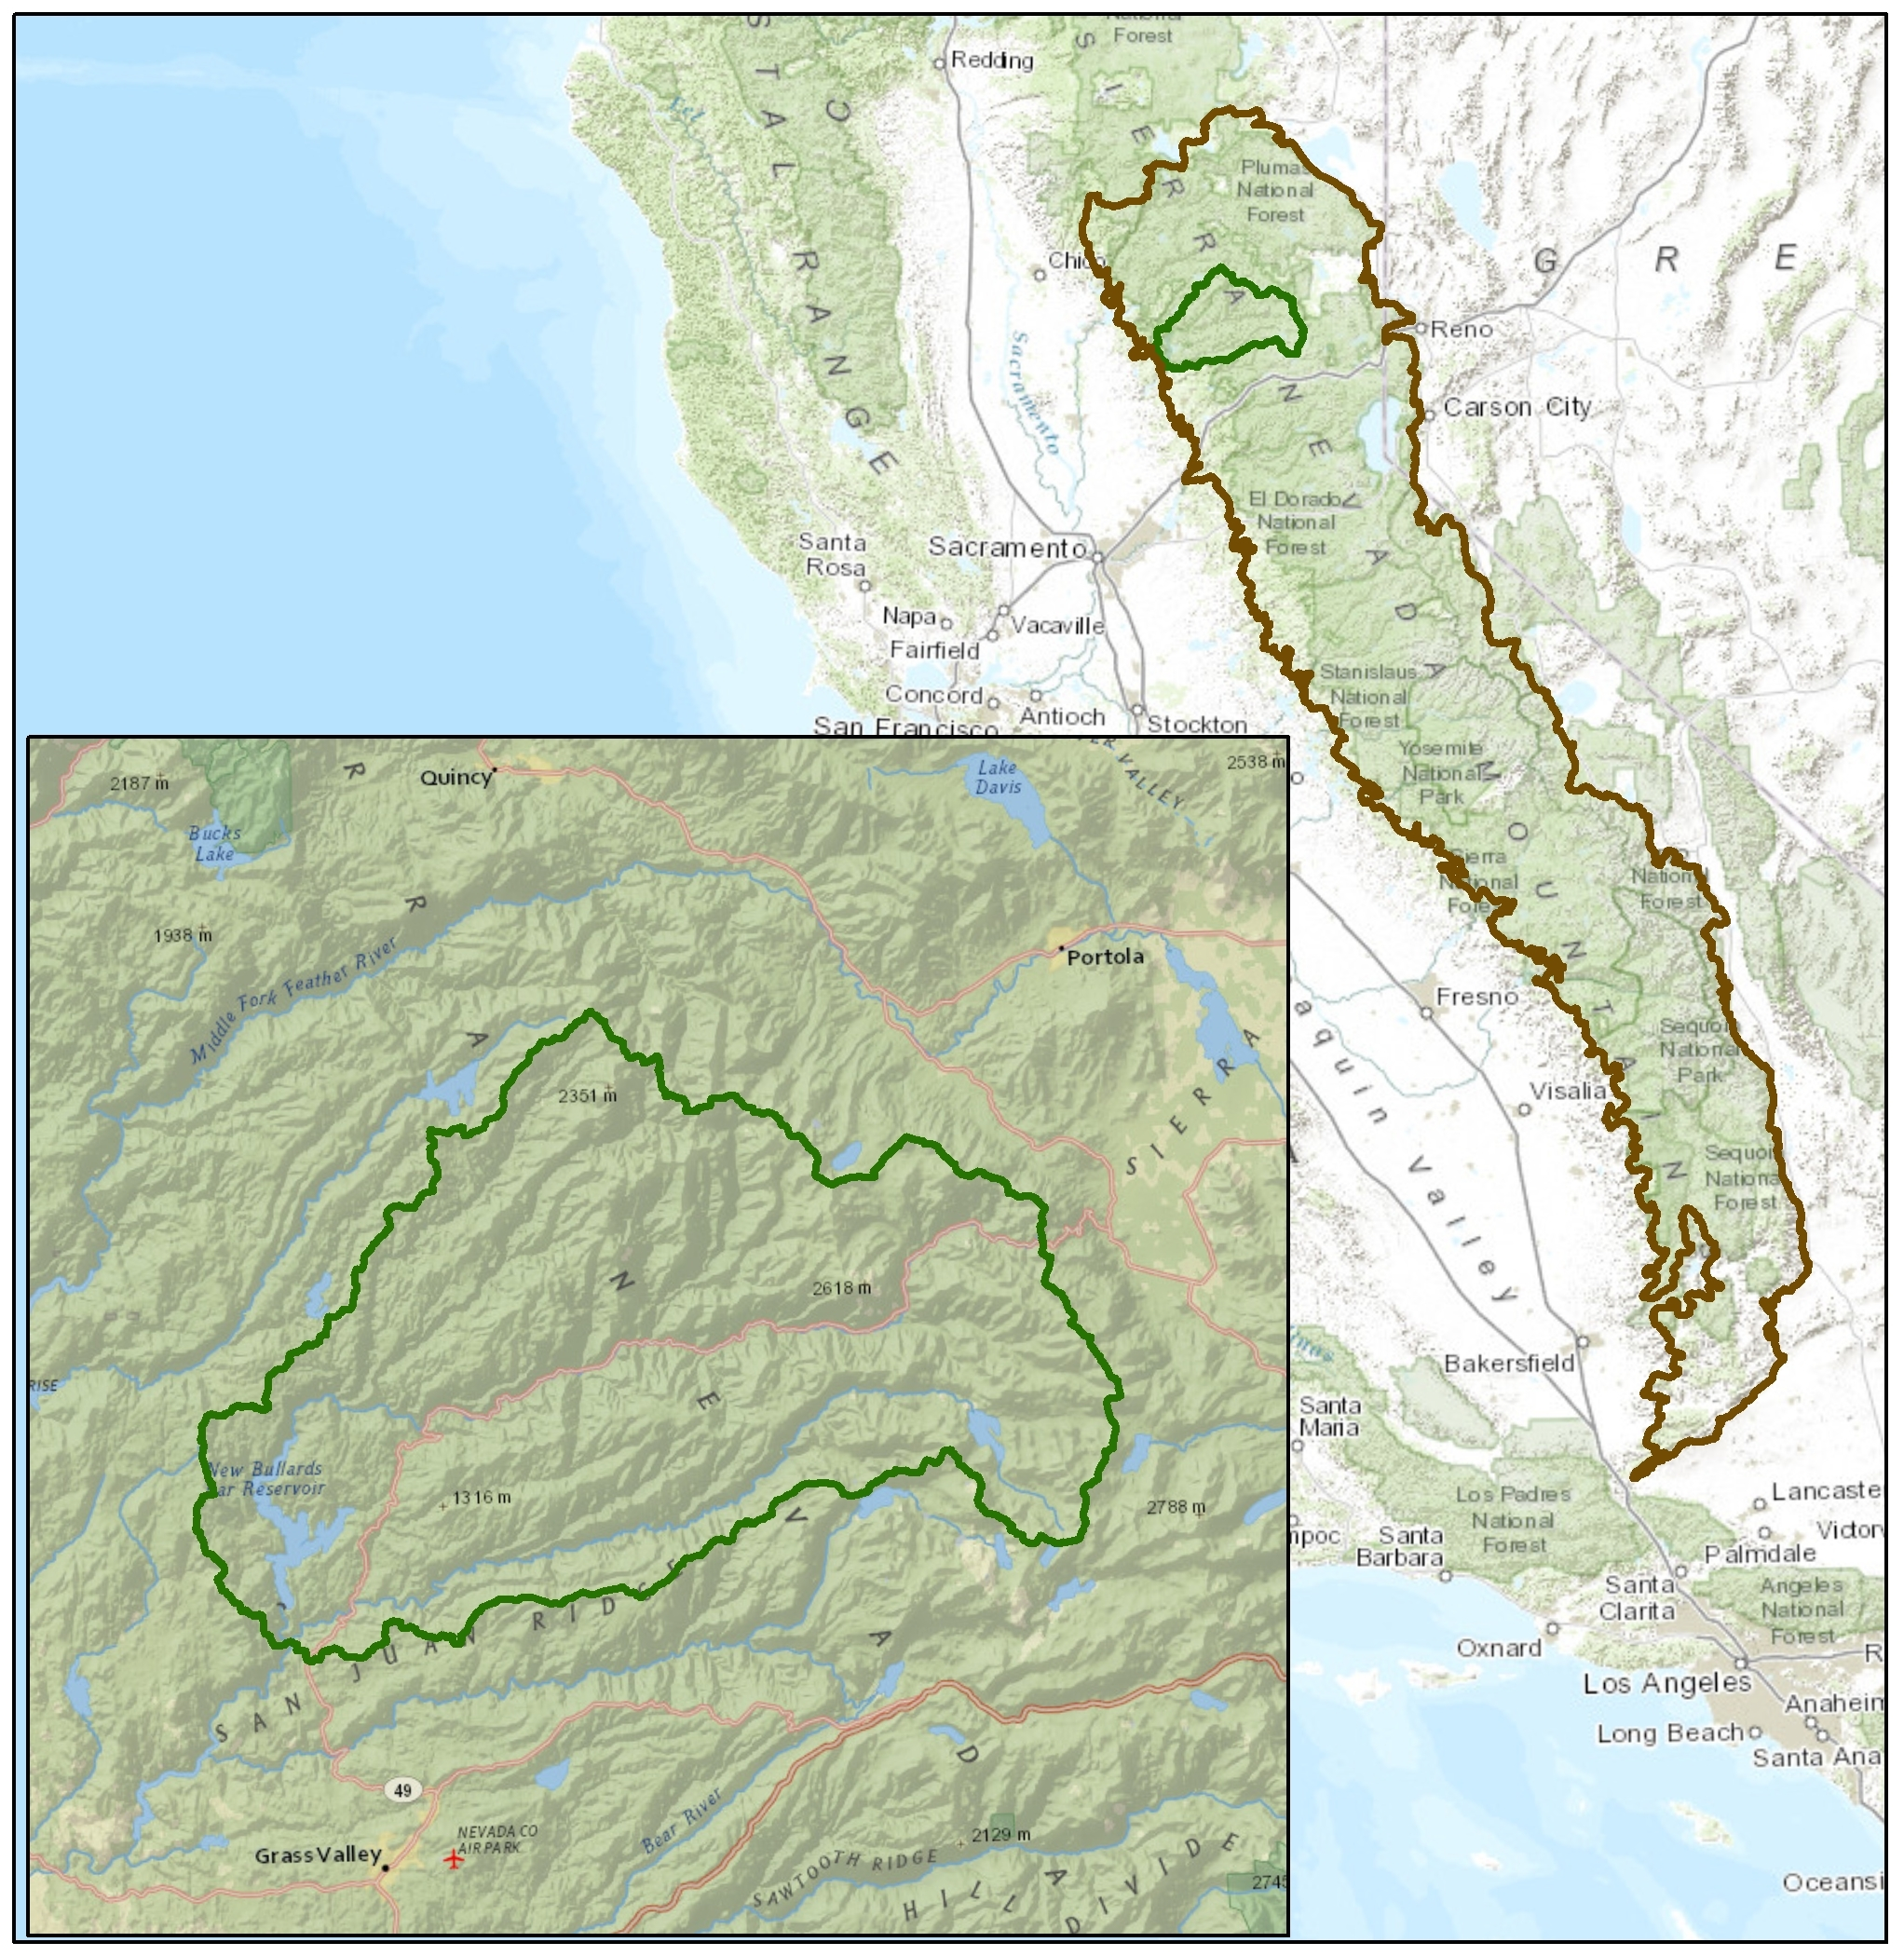
\includegraphics[width=\textwidth]{images/ecoregionprojectarea.jpg}
\caption{The Sierra Nevada Ecoregion is outlined in brown. The project landscape (outlined in green) is located in the northern extent of the Sierra Nevada on the Tahoe National Forest, comprising the Yuba River watershed.}
\label{projectarea}
\end{figure}

The Sierra Nevada is a major North American mountain range, located east of California's Central Valley and extending from Fredonyer Pass in the north to southern Kern County in the south. Much of the Sierra Nevada is reserved as federally-held public land, managed by the U.S. Forest Service, Bureau of Land Management, and the National Park Service. The Plumas and Tahoe National Forests are located in the northern portion of the Sierra Nevada. The project landscape (see Figure~\ref{projectarea}) is located on the northern part of the Tahoe National Forest, on the Yuba River and Sierraville Ranger Districts, and comprises about 181,550 hectares. It is composed of a set of three HUC-5 watersheds, the Upper North Yuba River, the Middle Yuba River, and the Lower North Yuba River, collectively referred to in this document as the Upper Yuba River watershed. 

The topography of the project landscape consists of rugged mountains incised by two major and a few minor river drainages. Elevation ranges from about 350 to 2500 meters. The area receives 30--260 cm of precipitation annually, most of which falls as snow in the middle to upper elevations (Storer and Usinger 1963). Some areas in the mid-elevation band receive high precipitation compared to the region, resulting in patches of exceptionally productive forest (Alan Doerr, pers. comm.). Vegetation is tremendously diverse and changes slowly along an elevational gradient and in response to local changes in drainage, aspect, and soil structure. Grasslands, chaparral, oak woodlands, mixed conifer forests, and subalpine forests are all found within the study area. Many species exhibit fire-adapted traits, such as resprouting from roots after a fire (e.g. tanoak), fire-induced germination (e.g. manzanita), or thick bark (e.g. ponderosa pine). 

Prior to European settlement, wildfire was a major source of disturbance on the landscape, shaping the composition and configuration of vegetation in the Forest. Fires were primarily lightning-caused, although indigenous peoples are thought to have set fires for vegetation management, especially in the lower elevations. In general, fire was frequent, with a mean rotation as short as 20 years in Ponderosa Pine-dominated forests. Wetter mixed conifer areas are predicted to have had a mean fire rotation of 30 years. Fire rotation is thought to increase gradually with elevation. For example, mesic Red Fir forests, which exist around 2,000 feet higher in elevation than Ponderosa Pine forests, had a mean fire rotation of 60 years. Variance around these means can be significant, as some parts of the forest experience fire much more frequently, while other escape fire for long periods. In general, regardless of vegetation type, high mortality fires were thought to be rare, with the vast majority of fires killing under 70\% of overstory trees. Under this disturbance regime, stand-replacing fire initiated early development conditions on the landscape. Low mortality fire tended to open forest canopies, especially in more xeric parts of the forest, while vegetation succession closed them again. The rarity of high mortality fire allowed large forest stands to succeed into late development and old growth conditions. \todo{How to cite this? At the end of the paragraph or repeatedly in it?}

The arrival of Europeans in the 1850s sparked a transformation of this landscape as people harvested timber, extracted gold using hydraulic mining techniques, and suppressed wildfires (Storer and Usinger 1963). Forestry, mining, grazing, and dozens of recreational activities, including hunting, mountain biking, and hiking continue to take place on the Tahoe National Forest. Fifteen allotments exist within the project area for both cattle and sheep grazing. In addition, 231,368 hectares inside of the project area have non-Forest Service ownership. Many of these lands were privately held, often by timber companies, before the Forest was created. In addition, many public lands were given to the Central Pacific Railroad in the late 19th century, and this ``checkerboard'' ownership pattern persists today (Figure~\ref{ownership}). Mining of gold and other minerals also continues. These activities affect and interact with ongoing vegetation succession and disturbance processes in the area. \todo{info easily found on forest website - need to cite?}

\begin{figure}[!htbp]
\centering
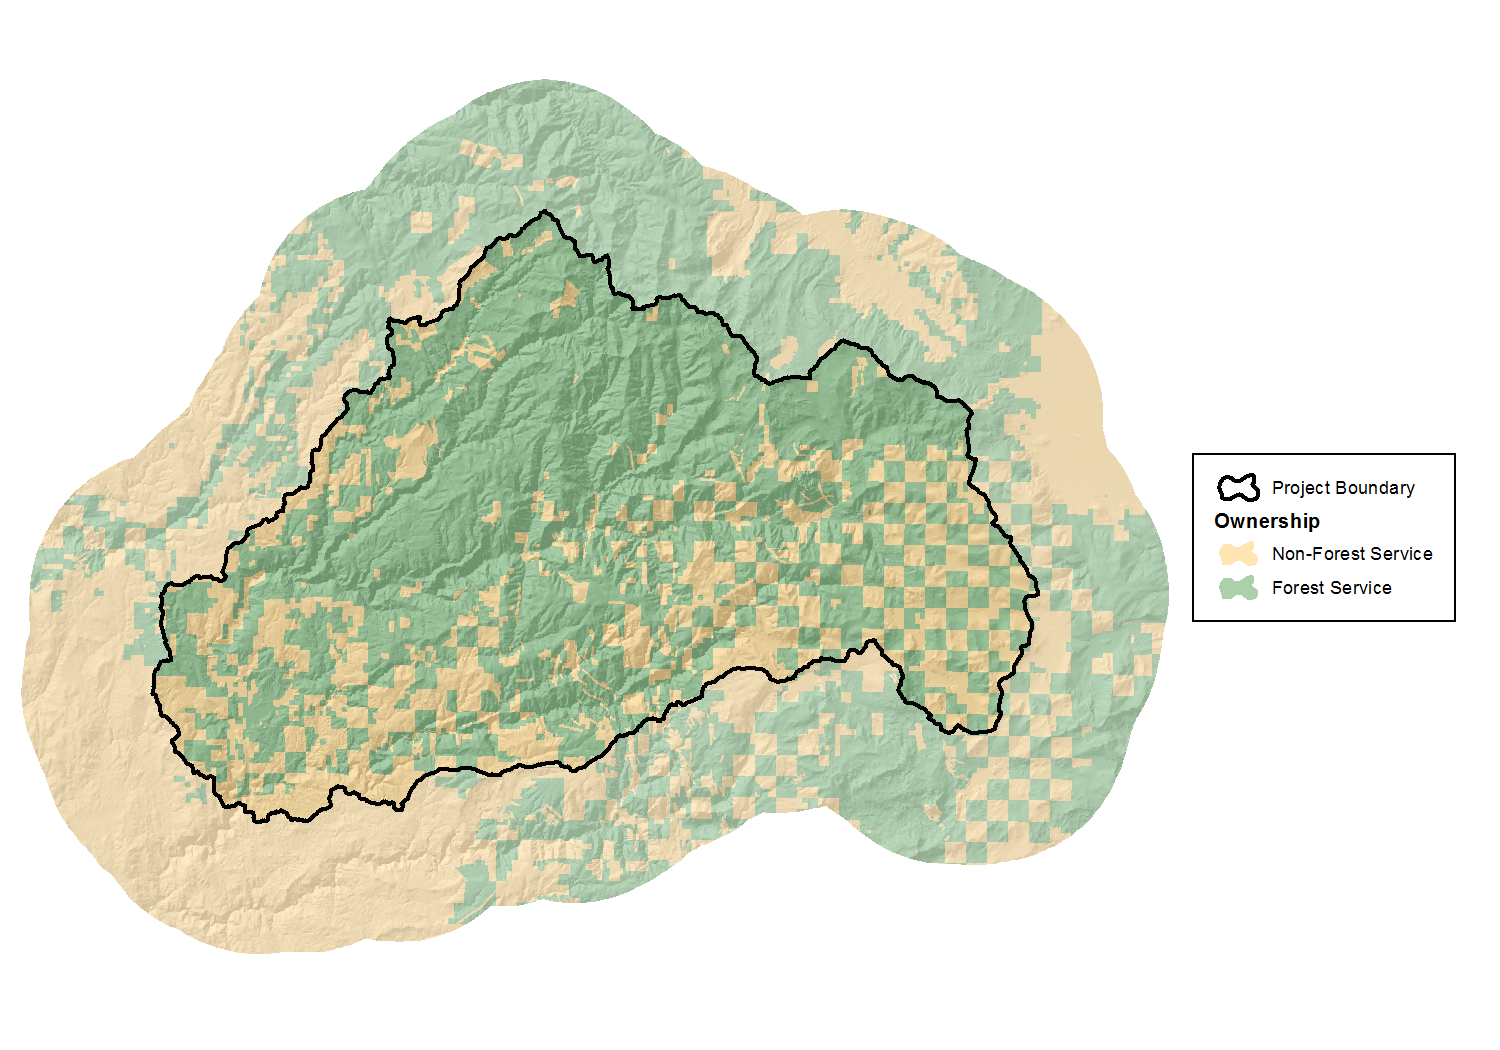
\includegraphics[width=0.8\textwidth]{/Users/mmallek/Tahoe/Report2/images/ownership.png}
\caption{Map distinguishing between National Forest lands and lands held by other entities (including private, industry, and other public land).} 
\label{ownership}
\end{figure}

The Tahoe National Forest has an active fire management program, and maintains a cooperative agreement with the State of California to help fight wildfires on the non-Forest Service lands located with the Forest boundary. In the recent history of the forest, very few acres have burned, with the exception of 1960, when approximately 100,000 acres burned on the Forest. The low burned acreage corresponds with fairly high fire starts (both human- and lightning-caused) [Forest Plan]. Fire suppression has lead to an increase in the amount of dead and downed fuels in the forest (SNFramework).

Logging has been a major human impact on the Forest since European settlement. Clearcutting, shelterwood, salvage cutting, and plantation management have been major components of timber management on the TNF for several decades. More recently, group cut strategies replaced clearcutting as a management alternative. Together with fire suppression, timber management on the Forest has effected changes in forest composition. In general, shade intolerant species such as ponderosa pine, sugar pine, and Douglas fir have become less common, while shade tolerant species, especially white fir, have become more predominant [1990 Forest Plan]. In the last 20 years, timber sales in the Sierra Nevada have dropped drastically, but on the Tahoe National Forests timber sale levels have fluctuated both up and down (although annual sawtimber sold has decreased similarly to other Sierran Forests).


\section{Modeling Framework}
\label{sec:modelframe}

\section{Historic Range of Variability}

\subsection{Input Layers}
\label{subsec:hrvinputlayers}

\paragraph{Data Structure} \textsc{RMLands} uses raster GeoTiffs (.tif files) as its data structure. Rasters are based on uniform square units called cells (or pixels). Each cell represents an actual portion of geographic space, where each cell has a defined X and Y value that corresponds to the coordinates defined by the projection. For example, in the Universal Transverse Mercator (UTM) projection, the grid that covers the entire Tahoe and Plumas National Forests project area is in UTM Zone 10 North and covers an area defined by a range of X and Y values (minimum and maximum).\footnote{Latitude and longitude are commonly pictured when describing coordinates. In such cases the X value refers to longitude and Y refers to latitude. However, because we use UTMs in this project, the correct convention is actually that the X value is the Easting and the Y value is the Northing. For simplicity we discuss X and Y only in this document.} In the Yuba River watershed landscape, each grid cell is 30 meters on a side (i.e., 900 m$^2$ or 0.09 ha), and the input grid measures 2910 by 2245 pixels. All grids must be single-attribute, signed integer grids. In other words, each cell is assigned a single class value, where valid class values are positive or negative whole numbers. All grids are created in ArcMap and saved as GeoTitff files before being input to the model. 

\paragraph{Raster layer alignment} \textsc{RMLands} requires that all grids are perfectly aligned. This means that not only must all grids have the same cell size and the same numbers of rows and columns, but the cells need to occupy the exact same geographic space and have the same number of total cells. \textsc{RMLands} requires that all input grids are perfectly aligned. We accomplished this by setting the Extent and Snap Raster to the same parameters whenever we manipulated the layers in ArcMap. This ``base'' spatial layer was created by taking the primary elevation layer used on the Tahoe National Forest, resampling it to a 30 meter grid, and clipping its extent to match that of the buffered project area.

The input layers are: cover, condition, age, aspect, slope, elevation, streams, roads, and condition-age.

\todo{Could also put all the maps of these layers on one page, as part of 1 large figure. Either 4 or 6 to a page.}

\subsubsection{Cover} The \emph{cover} layer represents land cover type, which is often but not always the vegetation type (i.e. cover types include not only Lodgepole Pine, but also Barren, and Agriculture). \emph{Cover} does not change over time, and is used to define several model parameters, including susceptibility to disturbance initiation or spread, and potential transitions between \emph{condition} classes undergone by cells within a particular cover type.

Cover represents land cover type. Typically, cover type is based on the potential or current natural vegetation of a site and may include both natural and anthropogenic cover types. For example, cover types include not only Lodgepole Pine, Sierran Mixed Conifer, and Red Fir, but also Barren and Agriculture. Cover affects virtually every process in \textsc{RMLands}. Succession pathways are defined uniquely for each cover type, susceptibility to natural disturbances varies among cover types, and suitability or eligibility for various vegetation treatments varies among cover types. Cover is a \emph{static} grid. Specifically, cover provides a fixed template upon which disturbance and succession processes play out over time. The cover type of a cell does not change over time; it is constant. All cells within the project boundary must be assigned a cover type; i.e., there can be no missing data or ``background'' within the project boundary. NODATA is reserved for all cells outside the project boundary.

The source for the cover layer is the Region 5 Existing Vegetation Layer (``EVeg''), mapped to the CALVEG classification developed by the Region's Ecology Program in 1978. The CALVEG types in the project area are specific to the North Sierra mapping Zone. Within the project area, the EVeg layer was developed based on three separate efforts: a satellite-based imagery analysis in 2000, and two orthoimagery analysis completed by contracting firms in 2005. Generally, specific cover type names were derived from the California Fire Return Interval Departure (FRID) report by Safford et al. \todo{Citation}

\paragraph{Alternative Cover Layers}
The original intent of our team was to utilize two separate cover layers: one for the historical reference period, and one for the current period to be used in projections of future scenarios. Two layers were identified as potentially suitable for the historic analysis: a map created from forest survey and inventory efforts under Albert Wieslander conducted between 1928 and 1940 (``Wieslander'') \todo{cite CEC}, and a map of Potential Natural Vegetation created by a Forest Service Enterprise Team for the Tahoe National Forest in the 2000s (``PNV''). Our intent was to use the PNV, Wieslander, or a combination thereof to derive the land cover layer for the HRV phase of the project. 

In order to validate the historical maps, we needed to develop a crosswalk between the vegetation type methodologies for the EVeg, PNV, and Wieslander maps. We also examined the spatial consistency in cover types across the maps. With significant assistance from the Tahoe National Forest, we attempted to create a crosswalk from these maps to the set of land cover types to be used in the project. However, we were unable to develop a consistent and comprehensive set of rules for this purpose. A major reason for this is that both the PNV and Wieslander maps used species lists, rather than assemblages (like in CalVeg and LandFire). For example, Sierran mixed conifer forests do not appear as a dominant ``cover type'' in the PNV map. The Wieslander maps do contain an internal crosswalk to a mixed conifer alliance, but only rarely. 

In addition, the PNV map contained a more significant error: we learned that, for the purposes of the modeling used to create the PNV map, ``potential natural vegetation'' meant the so-called ``climax'' community that would develop in the complete absence of disturbance, regardless of whether that disturbance was human-caused or natural. Since we are seeking to mimic the natural historic range of variability, we decided to discard this layer. The Wieslander map had its own issues. Most problematic was the non-systematic spatial error of up to 300 meters, which meant it would not be suitable for comparing specific locations. In addition, crosswalking precisely was impossible because coded vegetation was not necessarily in order of most prevalent vegetation, but instead prioritized tree species of shrubs, and commercially important trees over others. As an example from the handbook states, a plot consisting of 75\% \emph{Quercus kelloggi} (black oak), 15\% \emph{Pinus ponderosa} (ponderosa pine), and 10\% \emph{Pinus lambertiana} (grey pine) would be coded as ponderosa pine, grey pine, black oak. Consequently, the Wieslander map is also not a reliable predictor of land cover type without extensive review of the original data and maps, which would be beyond the scope of this project. 

To confirm these problmes, we examined the overlap in land cover types between different maps in ArcGIS. In general, the overlap between EVeg and either the PNV or the Wieslander layers was no better than random, and in many cases it was worse. We decided, in conjunction with Tahoe National Forest staff, to proceed using only the EVeg map, and omit the calibration period of the model from our analysis of the characteristics of the HRV. This ensured that our analysis of future management scenarios and comparison of spatial metrics between those results and the HRV results was credible.
% in retrospect I wonder if we should have analyzed the configuration more. in the end the biggest problem was probably the lack of crosswalk, since a precise spatial equivalence wasn't assumed.

\paragraph{Selection of Specific Cover Types}
In the early stages of this project, the team created a suite of land cover types based roughly on the Wildlife Habitat Relationships (WHR) types used in California and by Forest Service managers and planners. These consisted of the WHR types with a few additional types where additional specificity or refinement was desired. For example, Red Fir was split up into two subtypes. The original concept was to begin with the WHR types and modify them as needed based on other attributes in the EVeg layer. However, creating a crosswalk from WHR to the project-specific types also proved problematic. First, we realized that the WHR values were actually derived from the CalVeg species alliances included in the EVeg layer, but the methodlogy used was unavailable or missing. The crosswalks we did find \todo{cite} were not mutually exclusive and all-inclusive, and do not always make ecological sense. This is probably due in part to the fact that WHR is not a mapping classification. It is always derived secondarily. So, we were unable to create consistent rules for mapping from WHR to other types. Others have encountered similar issues:

\begin{quote}
WHR has been less successful in differentiating between vegetation types. Because the habitat types are inconsistently defined, a broad familiarity with its detailed descriptions is needed to differentiate among types of similar structure. Although mappers have constructed rules for discriminating among types, difficulties still remain because species dominance varies substantially within some types and broad overlaps in dominant plants occur among types. Other problems arise due to the small number of classes and the inconsistencies in scale among them \todo{(T. Veg of Cal)}
\end{quote}

With Tahoe National Forest staff we decided to instead base our land cover types on, at the first order, Presettlement Fire Regime (PFR) types as defined in the Fire Return Interval Departure (FRID)report by Safford et al. \todo{cite}. The PFR types, as part of the FRID, were developed through the scientific process and underwent peer review. We used the methodology from the FRID rather than using the second-order WHR classification and trying to reverse-engineer it to fit into our custom land cover types. Thus we created a new structure of cover types in a nested regime, moving from PFR (the coarsest aggregation of CalVeg types, which included a direct crosswalk from them to PFR types), to Biophysical Settings from LandFire (which were also crosswalked to PFR types in the FRID report), and finally to various local types not otherwise represented, such as xeric and mesic variants of cover types like Montane Hardwood, and aspen variants, such as Red Fir - Aspen. A mutually exclusive and all-inclusive crosswalk for each land cover type used in this analysis to a single LandFire Biophysical Setting and Presettlement Fire Regime type thus exists.

Extensive geoprocessing was required to prepare the EVeg layer for use in \textsc{RMLands}. Beyond converting the vector data to a raster format, further analysis was required to distinguish east- and west-side areas from one another, and generate the cover type modifications that the team agreed on. Aspen types were created by overlaying an aspen layer onto the vegetation layer and creating combined types (``type-aspen'')where appropriate. Areas mapped as a vegetation type characteristic of early seral (e.g. chaparral) were analyzed and assigned an appropriate forested cover type. Ultramafic types were created by overlaying a geology layer onto the vegetation layer and performing a similar processing step to create ``type-ultramafic''. Finally, for the Sierran Mixed Conifer and Red Fir cover types, which cover broad swaths of land across elevation and aspect, a xeric to mesic gradient was developed in conjunction with local experts and applied, creating ``type-mesic'' and ``type-xeric''. 

Ultimately, 31 cover types were generated for the buffered project area, as listed in Table~\ref{covertable} and shown in Figure~\ref{covermap}. A thorough description of geoprocessing steps necessary to recreate this data layer is available \todo{in forthcoming document?}. As Table~\ref{covertable} shows, most cover types occupy a small extent of the project area. The cover types with an extent of less than 1000 ha within the core project area may have statistically unreliable results; this problem increases as the extent of given cover type decreases. We caution against attempting to make inferences for these less common cover types. However, because the nine cover types that do occur over at least 1000 ha represent approximately 93\% of the core project area, we have high confidence in the landscape-level results.

%%%%%%%%%%%%%%%%%%%%%%
%%% COVER TABLE %%%%%%
%%%%%%%%%%%%%%%%%%%%%%
\small
\begin{table}[!htbp]
\caption{List of land cover types developed for this project. Included are the cover type abbreviation, full cover type name, and total area in the buffered project landscape in both acres and hectares.}
\label{covertable}
\begin{tabular}{@{}lllll@{}}
\toprule
\textbf{\begin{tabular}[c]{@{}l@{}}Land \\ Cover \\ Value\end{tabular}} & \textbf{\begin{tabular}[c]{@{}l@{}}Land Cover \\ Abbreviation\end{tabular}} & \textbf{Land Cover Name}                              & \textbf{\begin{tabular}[c]{@{}l@{}}Area \\ Core Only\\ (Hectares)\end{tabular}} & \textbf{\begin{tabular}[c]{@{}l@{}}Area\\ Core+Buffer\\ (Hectares)\end{tabular}} \\ \midrule
\rowcolor[HTML]{CAD6BA} 
1                                                           & AGR                                                                & Agriculture                                  & 16                                                          & 5,416                                                      \\
2                                                           & BAR                                                                & Barren                                       & 2665                                                        & 8,751                                                      \\
\rowcolor[HTML]{CAD6BA} 
3                                                           & CMM                                                                & Curl-leaf Mountain Mahogany                  & 18                                                          & 41                                                         \\
4                                                           & GRASS                                                              & Grassland                                    & 1379                                                        & 4,617                                                      \\
\rowcolor[HTML]{CAD6BA} 
5                                                           & LPN                                                                & Lodgepole Pine                               & 837                                                         & 2,816                                                      \\
6                                                           & LPN\_ASP                                                           & Lodgepole Pine with Aspen                    & 8                                                           & 31                                                         \\
\rowcolor[HTML]{CAD6BA} 
7                                                           & LSG                                                                & Black and Low Sagebrush                      & 0                                                           & 5                                                          \\
8                                                           & MED                                                                & Meadow                                       & 1201                                                        & 3,435                                                      \\
\rowcolor[HTML]{CAD6BA} 
9                                                           & MEG\_M                                                             & Mixed Evergreen - Mesic                      & 7273                                                        & 13,547                                                     \\
10                                                          & MEG\_U                                                             & Mixed Evergreen - Ultramafic                 & 604                                                         & 1,655                                                      \\
\rowcolor[HTML]{CAD6BA} 
11                                                          & MEG\_X                                                             & Mixed Evergreen - Xeric                      & 6768                                                        & 13,771                                                     \\
12                                                          & MRIP                                                               & Montane Riparian                             & 732                                                         & 2,216                                                      \\
\rowcolor[HTML]{CAD6BA} 
13                                                          & OAK                                                                & Oak Woodland                                 & 19                                                          & 4,186                                                      \\
14                                                          & OCFW                                                               & Oak-Conifer Forest and Woodland              & 23729                                                       & 56,941                                                     \\
\rowcolor[HTML]{CAD6BA} 
15                                                          & OCFW\_U                                                            & \begin{tabular}[c]{@{}l@{}}Oak-Conifer Forest and \\ Woodland -  Ultramafic\end{tabular} & 1060                                                   & 2,185                                                      \\
16                                                          & RFR\_ASP                                                           & Red Fir with Aspen                           & 0     		                                              & 34                                                         \\
\rowcolor[HTML]{CAD6BA} 
17                                                          & RFR\_M                                                             & Red Fir - Mesic                              & 8563  		                                              & 19,626                                                     \\
18                                                          & RFR\_U                                                             & Red Fir - Ultramafic                         & 294   		                                              & 321                                                        \\
\rowcolor[HTML]{CAD6BA} 
19                                                          & RFR\_X                                                             & Red Fir - Xeric                              & 7493  		                                              & 9,989                                                      \\
20                                                          & SAGE                                                               & Big Safebrush                                & 0     		                                              & 1,600                                                      \\
\rowcolor[HTML]{CAD6BA} 
21                                                          & SCN                                                                & Subalpine Conifer                            & 638   		                                              & 12,543                                                     \\
22                                                          & SCN\_ASP                                                           & Subalpine Conifer with Aspen                 & 0     		                                              & 6                                                          \\
\rowcolor[HTML]{CAD6BA} 
23                                                          & SMC\_ASP                                                           & Sierran Mixed Conifer with Aspen             & 58    		                                              & 121                                                        \\
24                                                          & SMC\_M                                                             & Sierran Mixed Conifer - Mesic                & 57853 		                                              & 133,920                                                    \\
\rowcolor[HTML]{CAD6BA} 
25                                                          & SMC\_U                                                             & Sierran Mixed Conifer - Ultramafic           & 4124  		                                              & 9,774                                                      \\
26                                                          & SMC\_X                                                             & Sierran Mixed Conifer - Xeric                & 52198 		                                              & 91,443                                                     \\
\rowcolor[HTML]{CAD6BA} 
27                                                          & URB                                                                & Urban                                        & 114   		                                              & 782                                                        \\
28                                                          & WAT                                                                & Water                                        & 4058  		                                              & 8,212                                                      \\
\rowcolor[HTML]{CAD6BA} 
29                                                          & WWP                                                                & Western White Pine                           & 273   		                                              & 510                                                        \\
30                                                          & YPN                                                                & Yellow Pine                                  & 0     		                                              & 10,499                                                     \\
\rowcolor[HTML]{CAD6BA} 
31                                                          & YPN\_ASP                                                           & Yellow Pine with Aspen                       & 0     		                                              & 3                                                          \\ \bottomrule
\end{tabular}
\end{table}
\normalsize

%\begin{verbatim}
%YHR	CellCount	Landcover3
%1	60173		AGR
%2	97233		BAR
%3	454			CMM
%4	51302		GRASS
%5	31289		LPN
%6	349			LPN_ASP
%7	50			LSG
%8	38171		MED
%9	150520		MEG_M
%10	18388		MEG_U
%11	153011		MEG_X
%12	24627		MRIP
%13	46514		OAK
%14	632677		OCFW
%15	24275		OCFW_U
%16	381			RFR_ASP
%17	218070		RFR_M
%18	3564		RFR_U
%19	110989		RFR_X
%20	17773		SAGE
%21	139365		SCN
%22	69			SCN_ASP
%23	1341		SMC_ASP
%24	1488003		SMC_M
%25	108605		SMC_U
%26	1016037		SMC_X
%27	8693		URB
%28	91245		WAT
%29	5668		WWP
%30 116653		YPN
%31	34			YPN_ASP
%\end{verbatim}

\begin{figure}[!htbp]
\centering
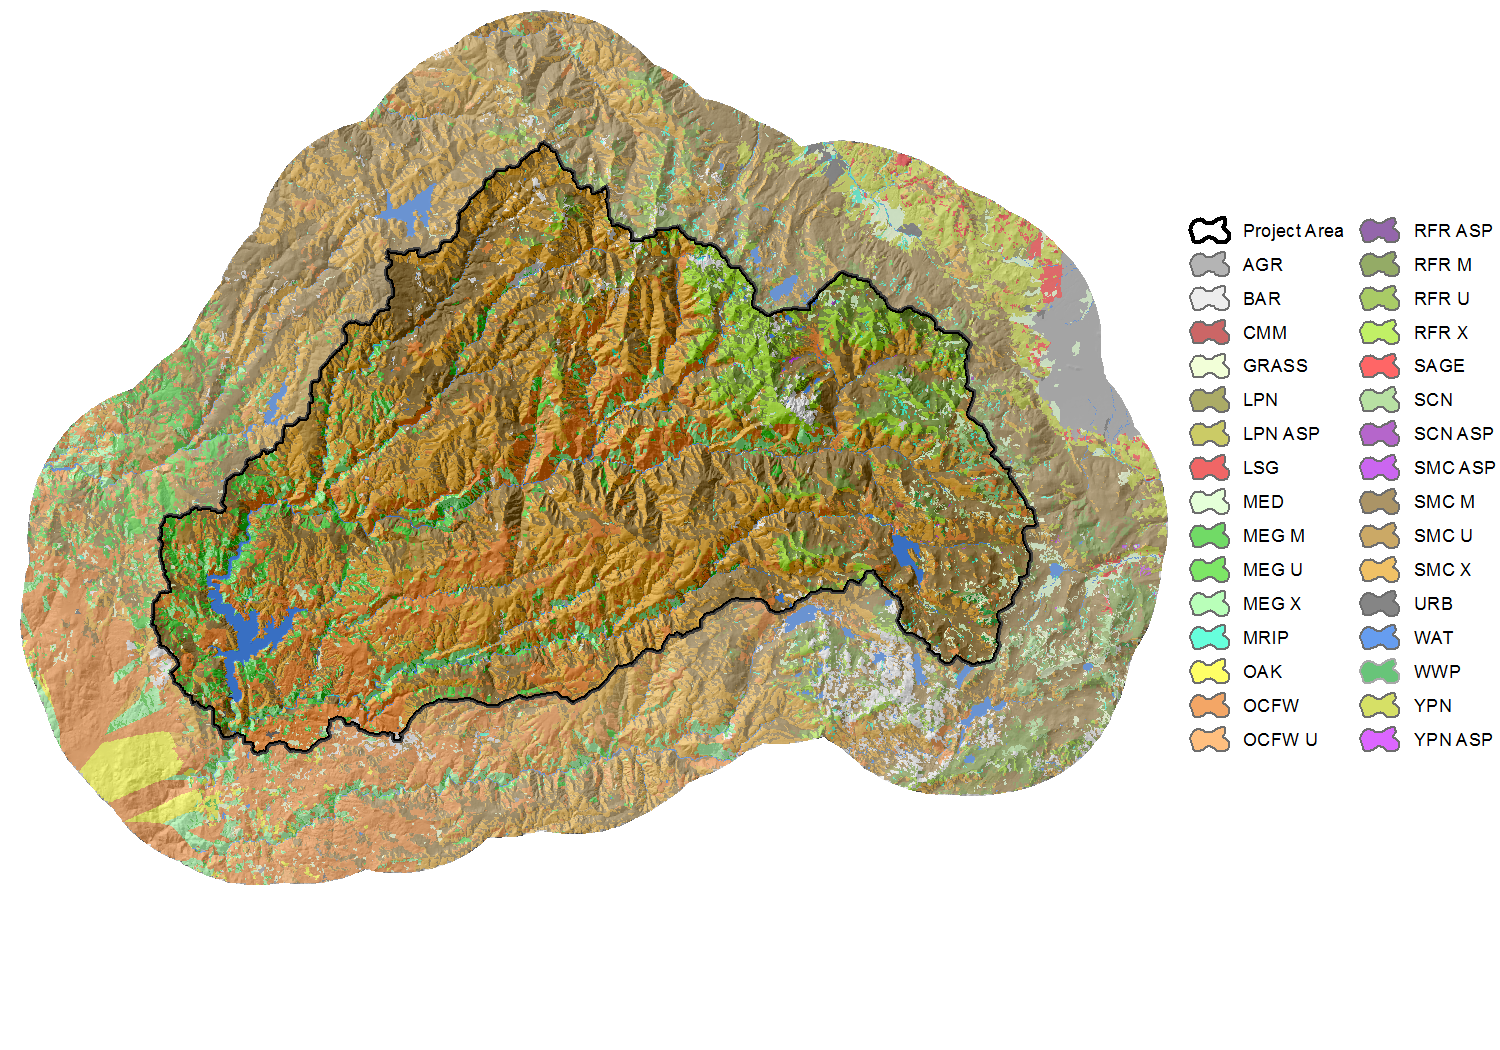
\includegraphics[height=0.4\textheight]{/Users/mmallek/Tahoe/Report2/images/cover.png}
\caption{Cover Type Map for the project area. Also shows the 10 km buffer from the project area boundary. See Table~\ref{covertable} for full land cover type names.} 
\label{covermap}
\end{figure}


\subsubsection{Condition}
Condition (or stand condition) class represents the structural condition of vegetation for cover types that undergo succession. Condition is a representation of discrete seral stages of stand development as identified by experts, which may vary considerably among cover types. It affects virtually every process in \textsc{RMLands}. In particular, transitions among condition classes during stand development define the succession pathways for each cover type. In addition, condition can be specified as a factor affecting susceptibility to natural disturbances and suitability (or eligibility) for vegetation treatments. Condition is a \emph{dynamic} grid; cell values change over time during the simulation in response to disturbance and succession processes. Ultimately, the combination of condition and cover defines the categorical classification of the landscape that provides the framework for characterizing vegetation patterns and dynamics. All cells within the project boundary are assigned a condition class; i.e., there is no missing data or ``background'' within the project boundary. However, some cover types (e.g., Urban, Agriculture, Meadow, etc.) may not have multiple condition classes and can be assigned a common value.

The source for the condition layer is the Region 5 Existing Vegetation Layer, mapped to the CALVEG classification developed by the Region's Ecology Program in 1978. Within the project area, the Existing Vegetation Layer was developed based on three separate efforts: a satellite-based imagery analysis in 2000, and two orthoimagery analysis completed by contracting firms in 2005. All members of the team discussed potential attributes to be used for this classification, and identified attributes for tree diameter at breast height (DBH) and cover from above (CFA) to classify pixels into early, middle, or late development, and open, moderate, and closed canopy. In this application, aspen and shrub types have condition classes that differ from that of the remaining forest types. The other forested types use a consistent set of condition classes.

Extensive geoprocessing was required to prepare this layer for \textsc{RMLands}. Beyond converting the vector data to a raster format, further analysis was required to update the layer to a year 2010 condition. Spatial data on wildfire and timber management history was used to provide a more accurate assessment of condition based on estimated stand age. In addition, areas currently mapped as chaparral in the Existing Vegetation Layer were assigned to the early development stage. The full set of condition classes is provided in Table~\ref{condtable} and depicted in Figure~\ref{conditionmap}.

%%%%%%%%%%%%%%%%%%%%%%
%%% CONDITION TABLE %%
%%%%%%%%%%%%%%%%%%%%%%

\begin{table}[!htbp]
\centering
\caption{List of condition classes developed for this project. Condition classes describe developmental stage (e.g. ``early'') and canopy closure (e.g. ``open''). Included are the condition class codes, abbreviations, and full names.}
\label{condtable}
\begin{tabular}{@{}lll@{}}
\toprule
\textbf{\begin{tabular}[c]{@{}l@{}}Condition Class \\ Value\end{tabular}} & \textbf{\begin{tabular}[c]{@{}l@{}}Condition Class \\ Abbreviation\end{tabular}} & \textbf{\begin{tabular}[c]{@{}l@{}}Condition Class  \\ Name\end{tabular}} \\ \midrule
\rowcolor[HTML]{CAD6BA} 
0                              & NS                                    & Non-Seral                     				 \\
10                             & EARLY\_ALL                            & Early Development - All                   	 \\
\rowcolor[HTML]{CAD6BA} 
20                             & MID\_CL                               & Mid Development - Closed                    \\
21                             & MID\_MOD                              & Mid Development - Moderate                  \\
\rowcolor[HTML]{CAD6BA} 
22                             & MID\_OP                               & Mid Development - Open                      \\
30                             & LATE\_CL                              & Late Development - Closed                   \\
\rowcolor[HTML]{CAD6BA} 
31                             & LATE\_MOD                             & Late Development - Moderate                 \\
32                             & LATE\_CL                              & Late Development - Open                     \\
\rowcolor[HTML]{CAD6BA} 
40                             & EARLY\_ASP                            & Early Development - Aspen                   \\
41                             & MID\_ASP                              & Mid Development - Aspen                     \\
\rowcolor[HTML]{CAD6BA} 
42                             & MID\_AC                               & Mid Development - Aspen Conifer             \\
43                             & LATE\_CA                              & Late Development - Conifer Aspen            \\ \bottomrule
\end{tabular}
\end{table}

\begin{figure}[!htbp]
\centering
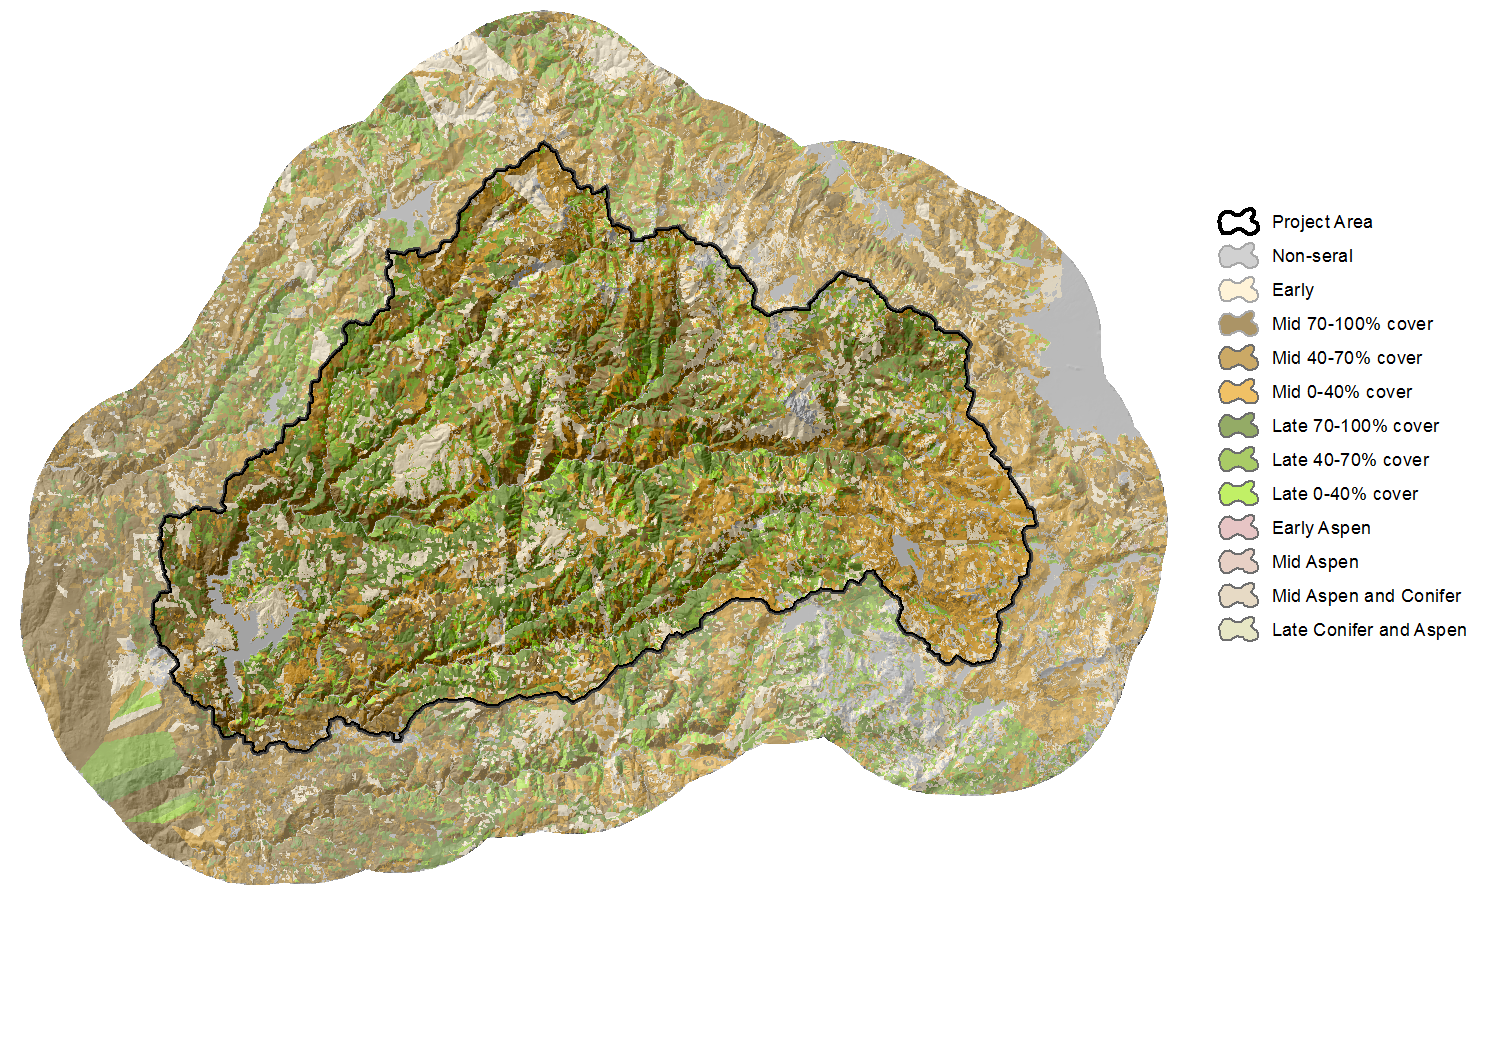
\includegraphics[height=0.4\textheight]{/Users/mmallek/Tahoe/Report2/images/condition.png}
\caption{Condition Class Map for the project area. Also shows the 10 km buffer from the project area boundary.} 
\label{conditionmap}
\end{figure}

\subsubsection{Age}
Age represents the number of years since stand origin (i.e., the number of years since the last stand-replacing disturbance), which is not necessarily the age of the oldest plant individuals in the stand. In some circumstances the age since stand origin can greatly exceed the age of the oldest individual plants (e.g., old-growth stands). It affects a variety of processes in \textsc{RMLands}, including succession transitions and susceptibility to disturbance. Age is a \emph{dynamic} grid; cell values change over time during the simulation in response to disturbance and succession processes. Age values can be any positive whole number, although any precision less than the length of the model time step (5 years) is inconsequential. In this application, we rounded all modeled and derived ages to the nearest five years. A ``no age'' value (99998) is assigned to all non-vegetated and non-seral cover types.

While Age is potentially an important variable in \textsc{RMLands}---for example, it is a factor influencing succession transitions and can provide a basis for summarizing the range of variability in vegetation conditions---the \emph{initial} age condition is a transient state that gets modified quickly during the simulation in response to disturbance and successsion processes. Therefore, the initial age structure of the landscape may be of little importance in a long-term simulation, as long as we properly account for the model equilibration period (i.e., the period it takes the age structure of the landscape to stabilize given the disturbance regime).

In this application, we used data from stand exams dating to the 1960s and from recent Forest Service Region 5 Ecology group survey plots to estimate stand age across the buffered project area. We then interpolated that information across the landscape. Due to insufficient data, we were unable to disaggregate the data below the landscape scale to cover type or another more finely resolved classification. We also acknowledge that the stand exam and modern veg plots do not constitute a true sample and were conducted almost exclusively in mid-mature and mature stands of commercially viable trees, thus skewing the results to some unquantifiable degree.

We updated the interpolated data with wildfire and timber management history, and assigned ages to types coded as chaparral in the Existing Vegetation layer to the midpoint of the age spread of early development for the forest cover type to which it was converted. Remaining ages out of compliance with allowed ages for the corresponding condition of a given cell were modified to be in compliance, based on the assumption that the condition class assignment was more accurate that the interpolated age information. The input Age layer, showing the map at timestep 0, is shown in Figure~\ref{agemap}.

\begin{figure}[htbp]
\centering
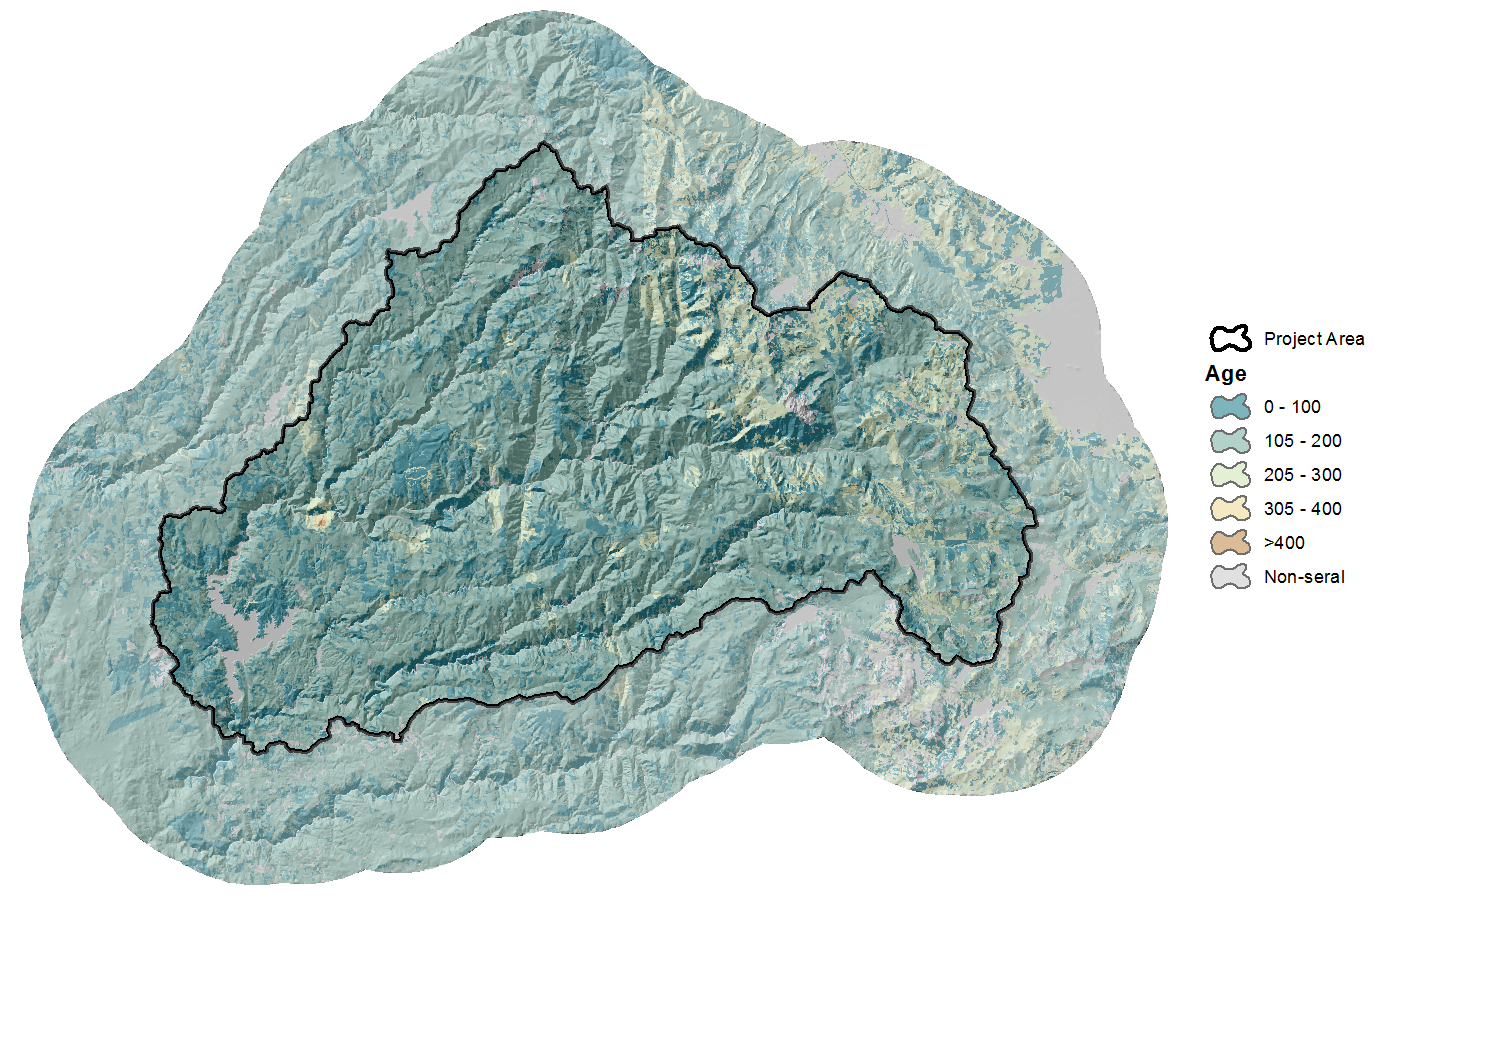
\includegraphics[height=0.4\textheight]{/Users/mmallek/Tahoe/Report2/images/age.png}
\caption{Age map at Timestep 0 for the project area. Also shows the 10 km buffer from the project area boundary.} 
\label{agemap}
\end{figure}

\subsubsection{Condition-Age}
Condition-Age represents the age since transitioning to the current condition. In \textsc{RMLands} it affects most transitions between condition classes: typically there is a threshold condition age below which transitions do not occur. After creating both the condition and age layers, we used a Python function to derive condition-age based on the youngest possible age for a cell of that cover and condition. For example, if we determine that a particular cell on the landscape has a cover type of Lodgepole Pine, condition of Mid Development Closed, and age of 50 years, we take the minimum age for that cover-condition combination (10 years old), and subtract it from the age to arrive at a condition-age of 40. The final, original map for the initial condition-age is shown in Figure~\ref{condagemap}.

\begin{figure}[htbp]
\centering
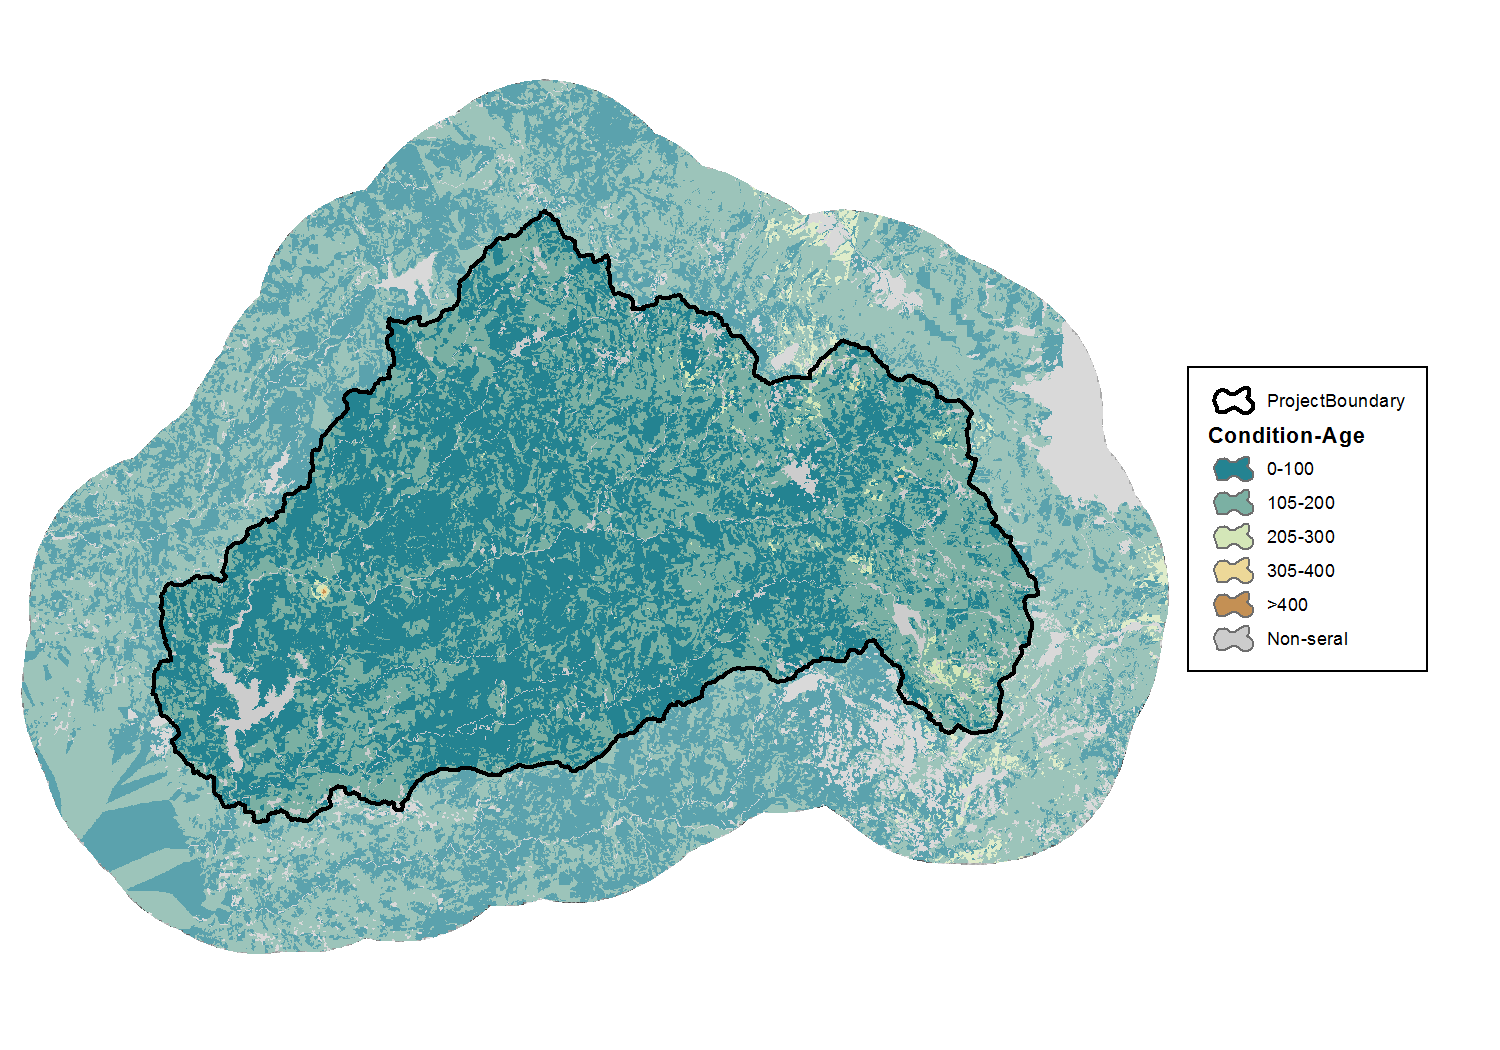
\includegraphics[height=0.4\textheight]{/Users/mmallek/Tahoe/Report2/images/condage.png}
\caption{Condition-Age map at Timestep 0 for the project area. Also shows the 10 km buffer from the project area boundary.} 
\label{condagemap}
\end{figure}

\subsubsection{Topographic Position Index}
Our topographic position index (TPI) combines heat load, which is based on aspect and slope, with slope position (Figure~\ref{tpimap}). High values for TPI are correlated with locations on steep, south and west-facing, upper slopes. Low values are correlated with locations on gentle, north and east-facing, valley bottoms. Values in between occur along a gradient of these characteristics. The TPI is scaled to the project area and the region immediately surrounding it, and is therefore a local index only. We use TPI to adjust vegetation susceptibility and mortality because we expect susceptibility and mortality to be higher when TPI is high.

\begin{figure}[htbp]
\centering
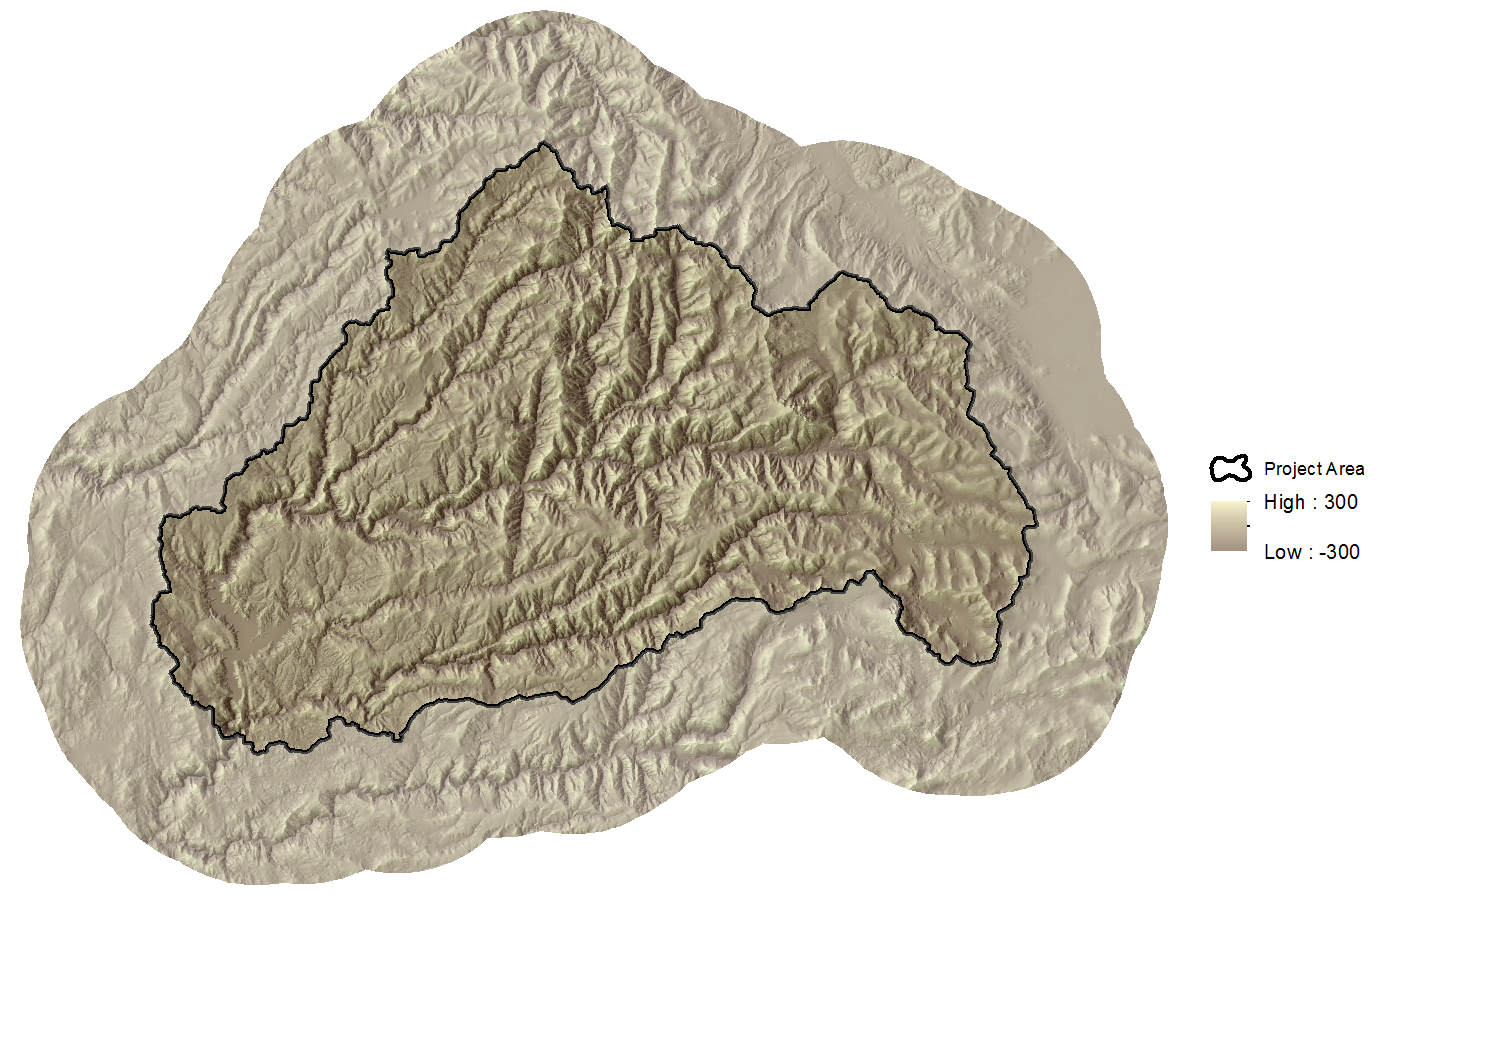
\includegraphics[height=0.4\textheight]{/Users/mmallek/Tahoe/Report2/images/tpi.png}
\caption{Topographic Position Index for the project area. Also shows the 10 km buffer from the project area boundary.} 
\label{tpimap}
\end{figure}

\subsubsection{Elevation} 
Elevation represents the height above sea level in meters. Elevation is typically derived from an existing digital elevation model (DEM). In \textsc{RMLands}, the elevation layer affects disturbance spread. \todo{Correct?} Elevation is a \emph{static} grid; cell values remain constant over time. The elevation grid used in this analysis was provided by the Tahoe National Forest GIS staff and rescaled from 10 m$^2$ to 30 m$^2$ pixels. It is shown as a map in Figure~\ref{elevationmap}.

\begin{figure}[htbp]
\centering
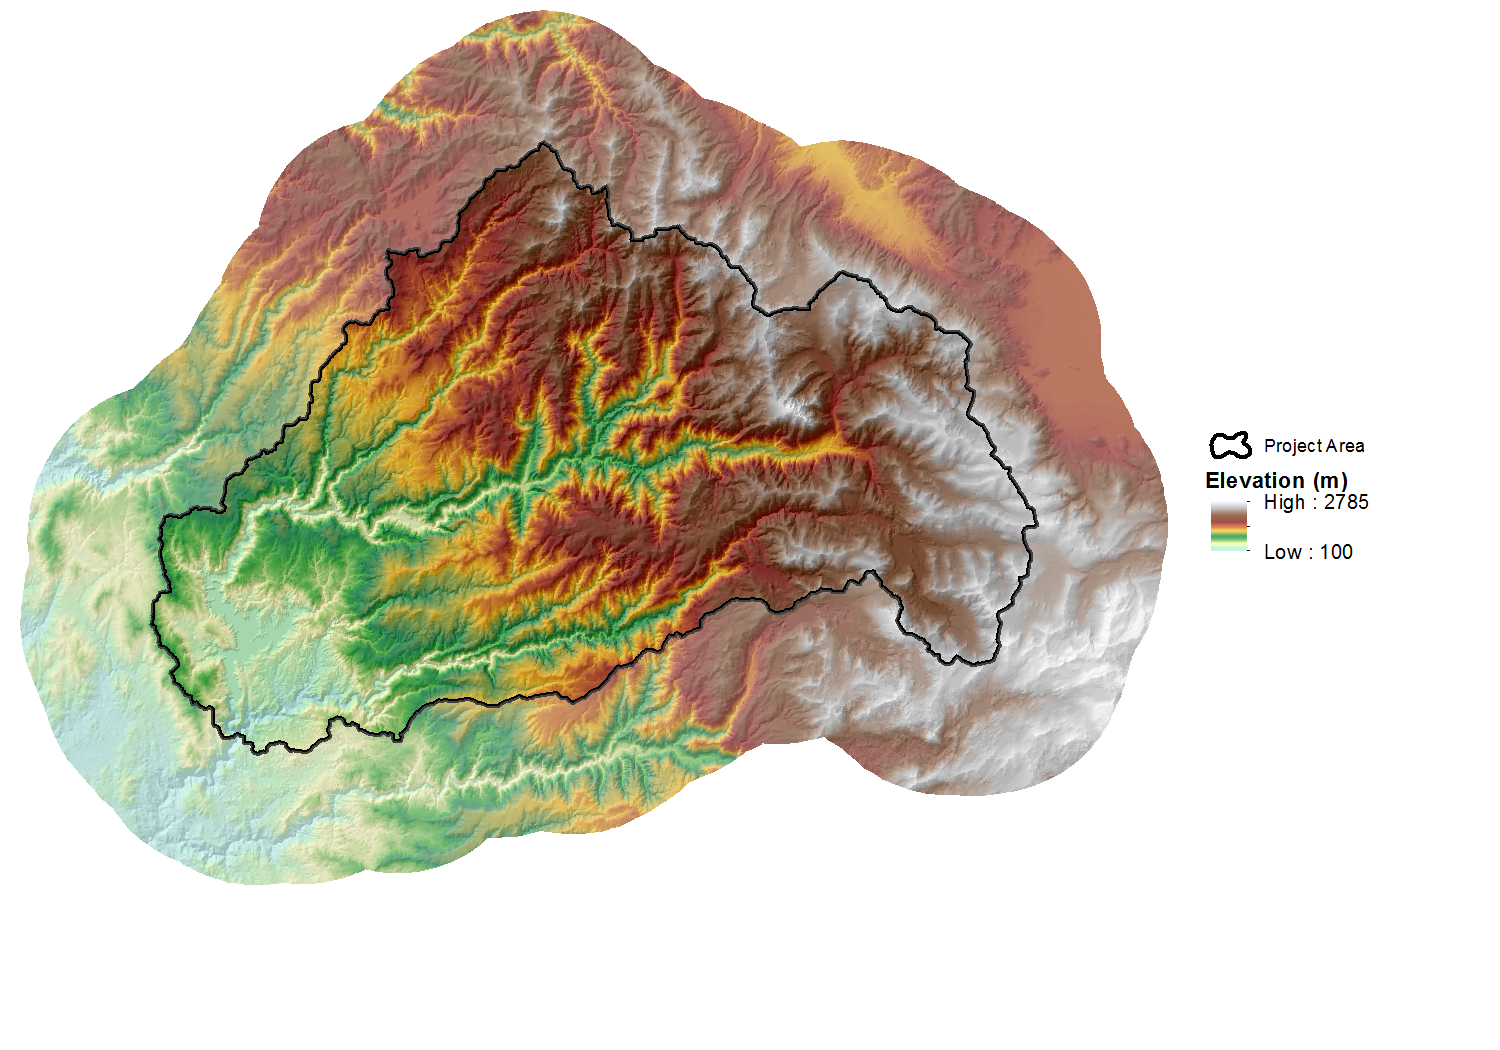
\includegraphics[height=0.4\textheight]{/Users/mmallek/Tahoe/Report2/images/elevation.png}
\caption{Elevation for the project area. Also shows the 10 km buffer from the project area boundary.} 
\label{elevationmap}
\end{figure}

\subsubsection{Slope} 
Slope represents the steepness of a cell as measured in percent and is derived from the elevation layer. Slope is used in GIS preprocessing to define cover types and eligibility for various vegetation treatments. Within \textsc{RMLands}, slope affects disturbance spread. Slope is a \emph{static} grid; cell values remain constant over time. The slope for the study area is shown in Figure~\ref{slopemap}.

\begin{figure}[htbp]
\centering
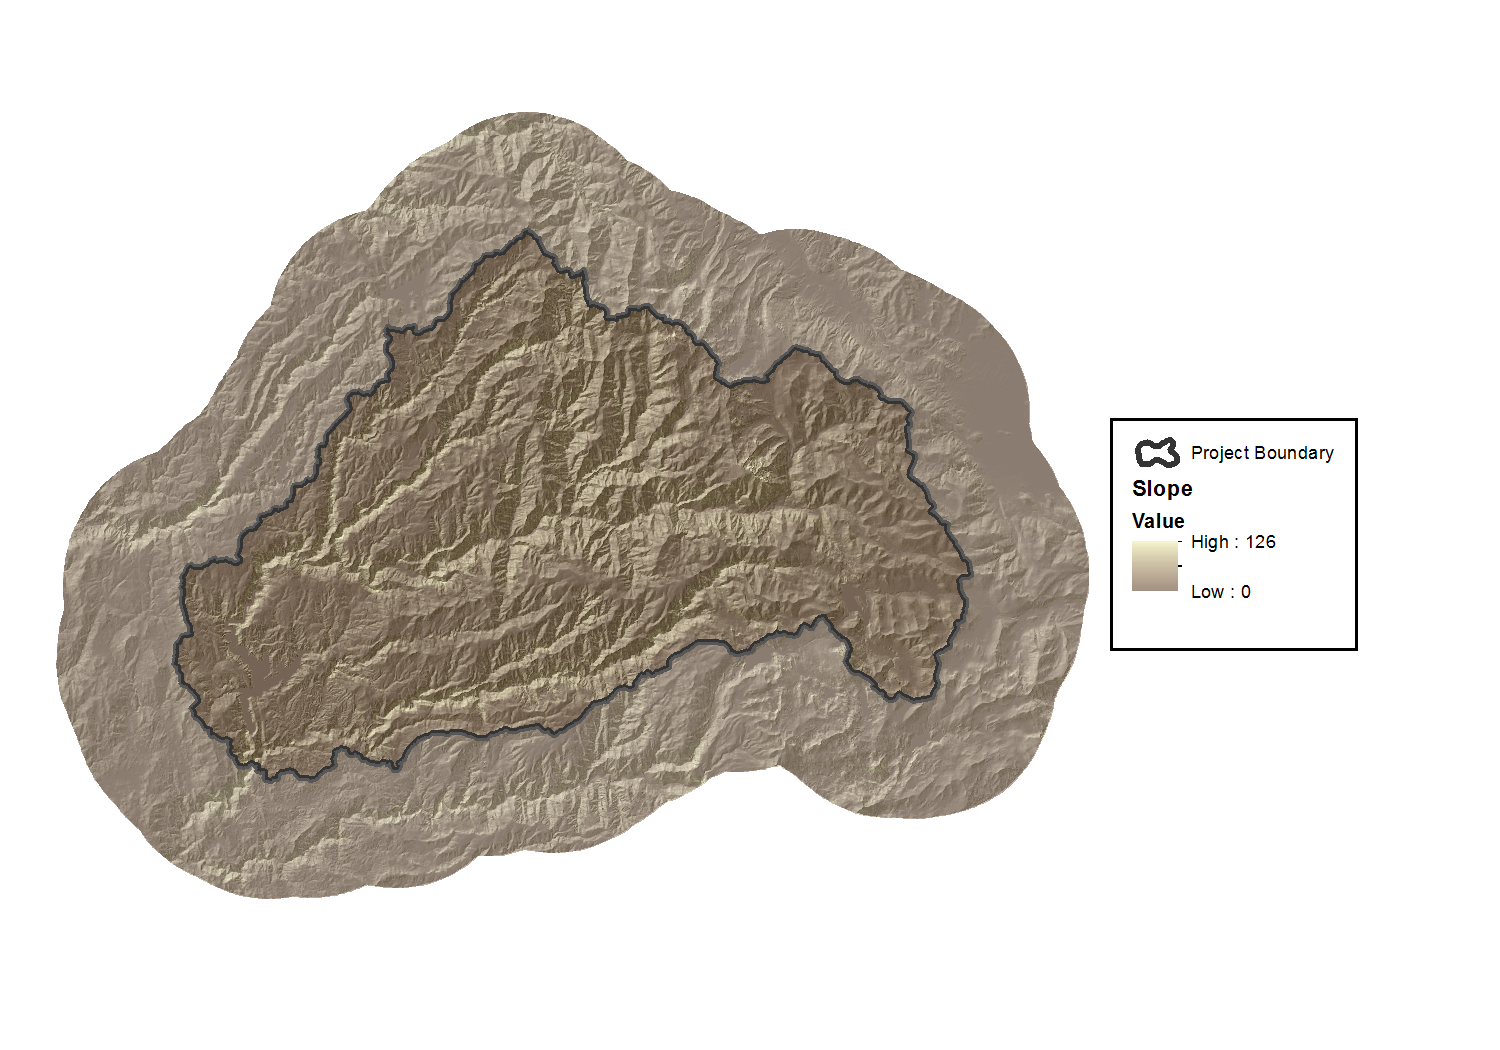
\includegraphics[height=0.4\textheight]{/Users/mmallek/Tahoe/Report2/images/slope.png}
\caption{Slope for the project area, which ranges from flat to 126\%. Also shows the 10 km buffer from the project area boundary.} 
\label{slopemap}
\end{figure}

\subsubsection{Aspect} Aspect represents the direction that a cell faces and is derived from elevation. It primarily affects the spread of disturbance in \textsc{RMLands}. Aspect is a \emph{static} grid; cell values remain constant over time. Grid values represent categorical values assigned to the eight cardinal directions, plus a value for flat areas with no aspect (see Figure~\ref{aspectmap}. 

\begin{figure}[htbp]
\centering
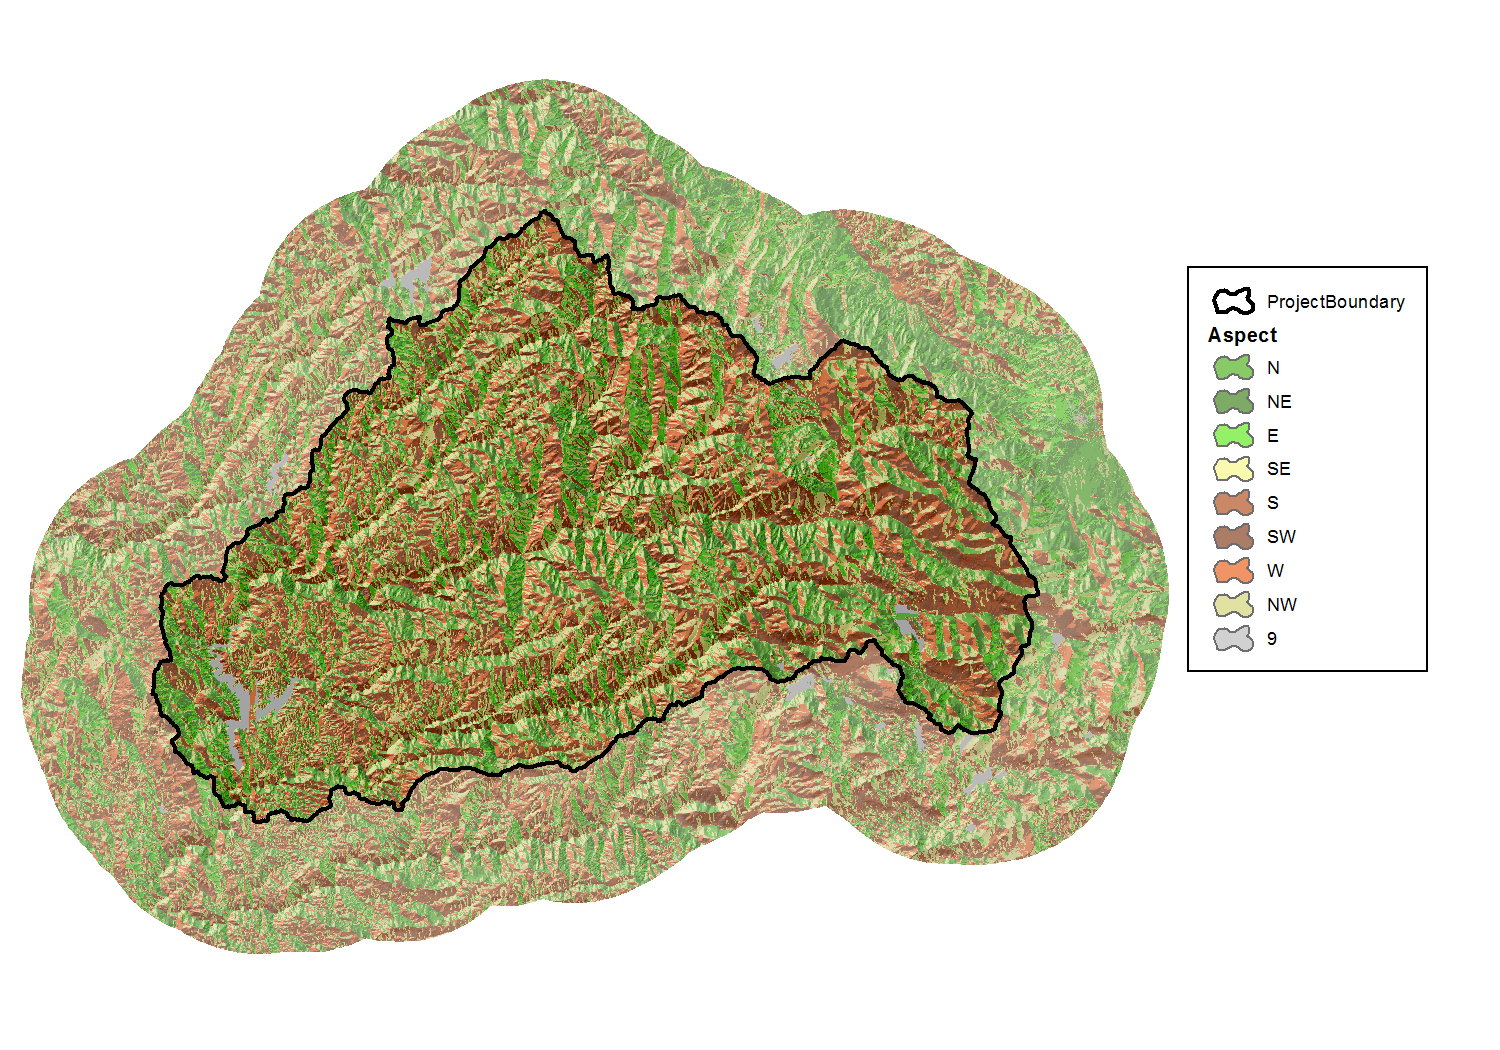
\includegraphics[height=0.4\textheight]{/Users/mmallek/Tahoe/Report2/images/aspect.png}
\caption{Aspect for the project area. Also shows the 10 km buffer from the project area boundary.} 
\label{aspectmap}
\end{figure}

\subsubsection{Streams} 
Streams represents aquatic communities classified as small, medium or large based on stream order. In this application, the streams layer was created from a line coverage containing hydrography data, including an attribute for stream size or order, by converting to a grid based on the stream size attribute. Streams are a potential barrier to the spread of wildfire disturbance in \textsc{RMLands}, or may be used as a natural boundary to a treatment unit, depending on their size.

We employed the orthogonal neighbor rule when converting a line to a raster of like-valued cells. That is, the final grid contains stream cells that connect along a cell side, as opposed to diagonally. This is required because diagonal neighbors, while touching, will not provide an impediment to disturbance spread (which happens diagonally as well as orthogonally). In addition, streams did not have to be in a contiguous network, which has implications in terms of disturbance spread and/or logical treatment boundaries; in general breaks in the stream network happens only near stream headwaters. 

Streams is a \emph{static} grid; cell values remain constant over time. Note, streams are integrated into the cover type classification scheme insofar as they are classified as type ``Water'' in the Existing Vegetation Layer. Regardless, they also exist as a single layer. Grid values represent categorical values assigned to the three stream size classes, plus a value for background. The final streams input layer is shown in Figure~\ref{streamsmap}.

\begin{figure}[htbp]
\centering
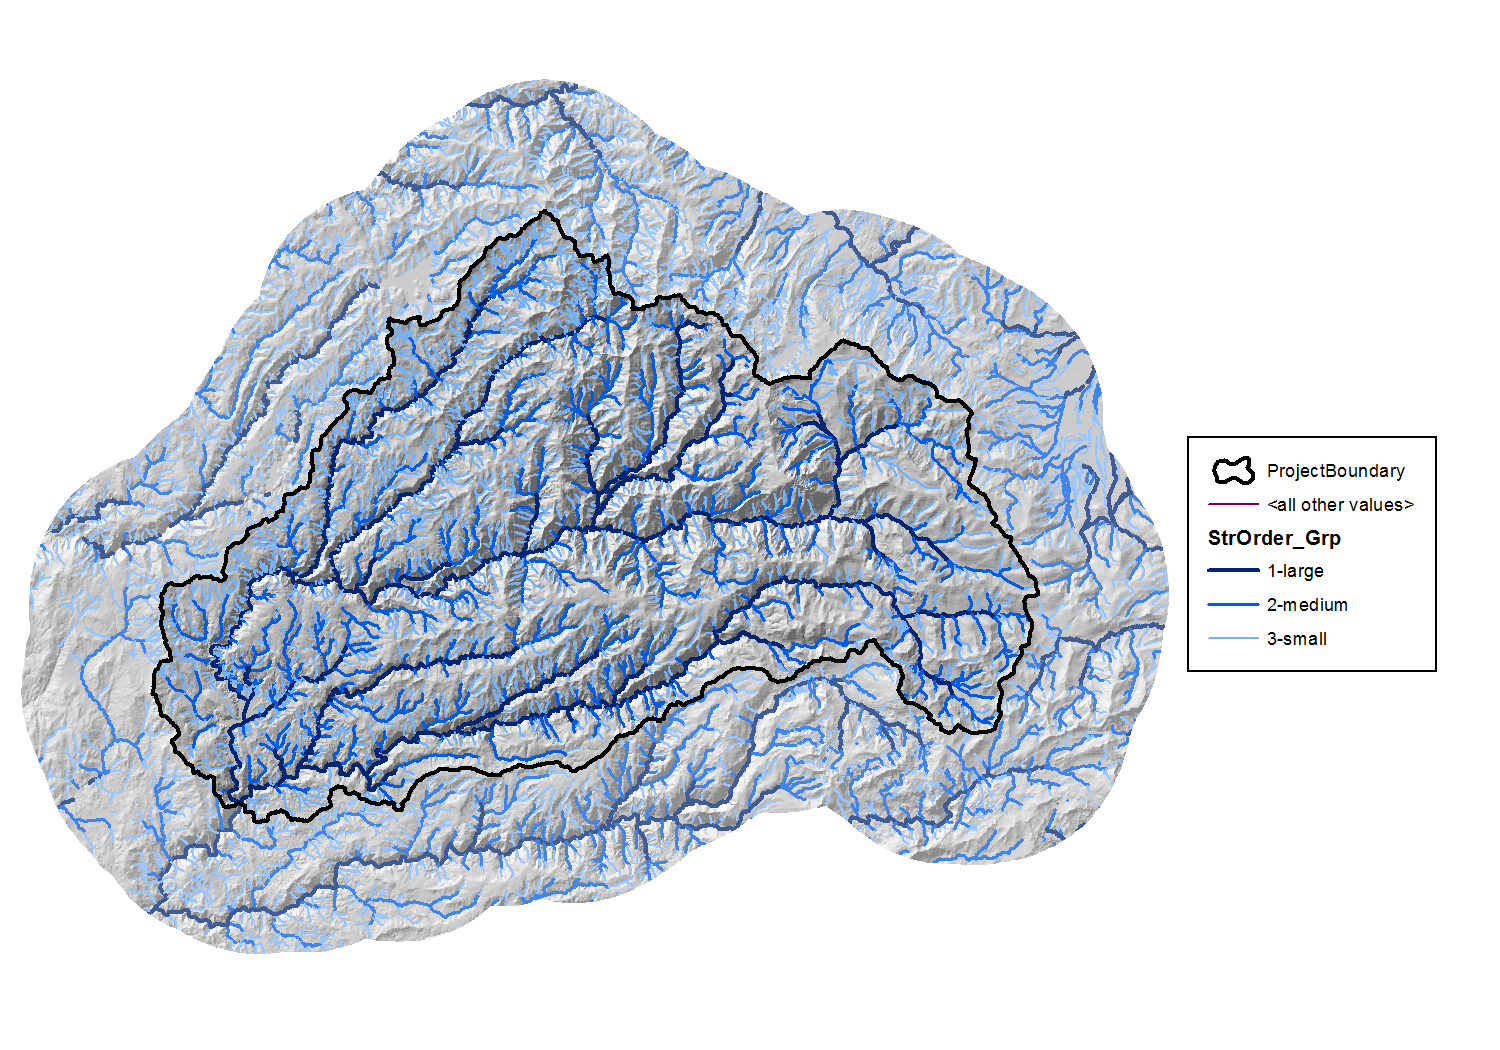
\includegraphics[height=0.4\textheight]{/Users/mmallek/Tahoe/Report2/images/streams.png}
\caption{Streams in the project area. Also shows the 10 km buffer from the project area boundary.} 
\label{streamsmap}
\end{figure}

\subsubsection{Buffer/Core} 
Buffer is a grid where the ``core'' project area is represented by one integer value, while its ``buffer'' around the core area is represented by a second integer value. The ``core'' area is the project area of interest (the watersheds), whereas the ``buffer'' is an arbitrarily-defined area around the core designed to eliminate the boundary (or edge) effect associated with disturbance spread. This allows disturbances to spread on to and off of the landscape without impediment. Without a buffer there is a substantial bias in the probability of disturbance for cells within a certain distance of the edge of the landscape because of the reduced likelihood that disturbances will spread to that location from outside the designated landscape. We use a 10 km buffer, which is generally sufficient to offset any boundary effects when simulating large wildfires. Because a buffer grid is specified, all other input grids must be classified within the full extent of the buffer area as well as the core. All succession and disturbance processes operate seamlessly across the buffer and core, and thus the presence of the buffer does not affect the simulation in any way. However, with the buffer present, all statistical reporting is restricted to the behavior in the core only. Buffer is a \emph{static} grid; cell values remain constant over time. The original polygon layer for this was generated by creating at 10km buffer around the project area watersheds. It was then converted to raster using the same procedure as for other layers. The buffer and core are easily distinguished in Figures~\ref{covermap}--\ref{streamsmap}: the core is the interior area delinated by a thick black line, while the buffer is area outside of this line, displayed at a decreased brightness level.



\subsection{Model Parameterization}
\label{subsec:hrvmodelparam}

\subsubsection{State and Transition Models}
We have created a detailed cover type description document for each cover type in the simulated landscape that experiences transitions between cover class. These documents describe crosswalks to other data layers, detailed accounts of the multiple species characteristic of the cover type, cover type distribution, relationship and response to wildfire, predicted fire return intervals, plus descriptions of each condition class present within the cover type and their succession and wildfire transition conditions and rates. \todo{APPENDIX?} Each detailed document can be summarized as a state and transition model for a particular cover type, which is implemented in the model by specifying susceptibility to wildfire, rules for vegetational succession, and rules for transitions after a fire event. Figure~\ref{transmodel} shows a generic example state and transition model for the forested cover types.

\begin{figure}[htbp]
\centering
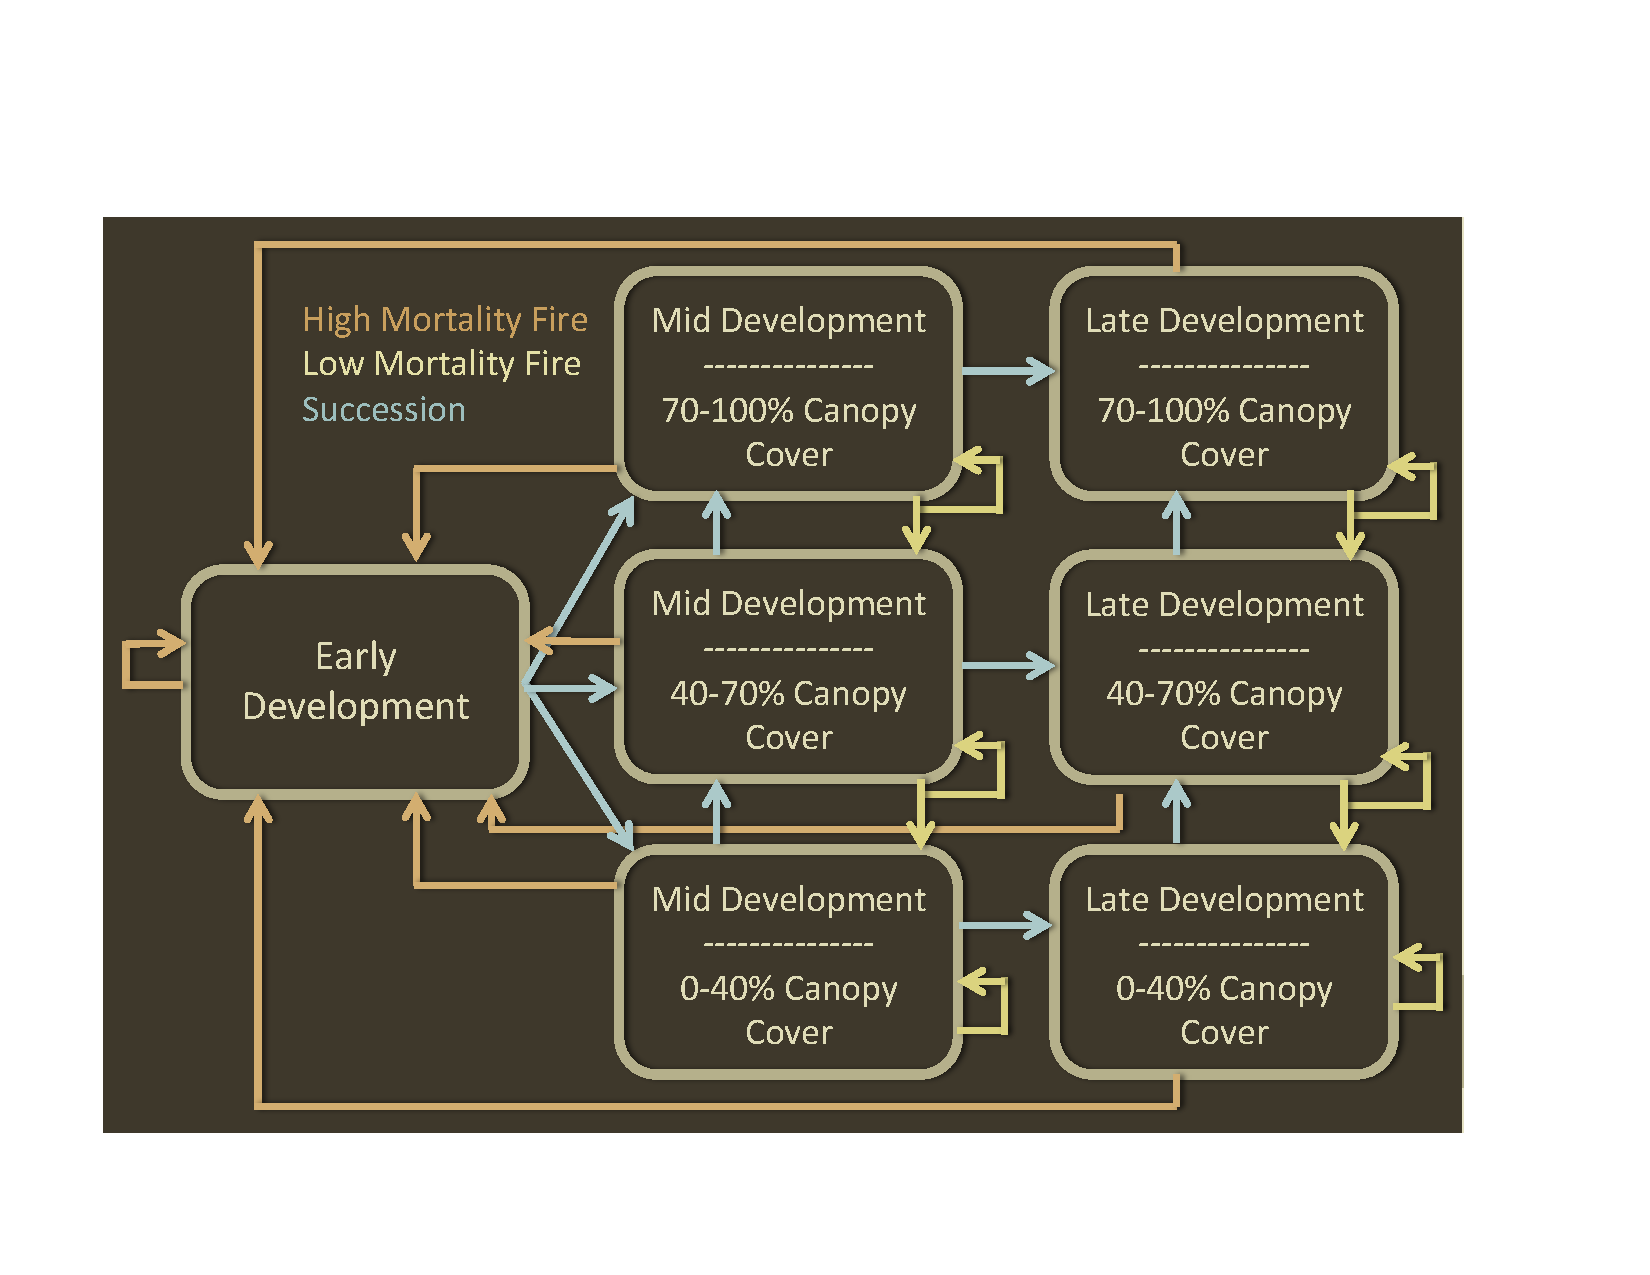
\includegraphics[width=0.8\textwidth]{/Users/mmallek/Tahoe/Report2/images/STModel_PowerPoint.pdf}
\caption{Generic state and transition model for all non-shrub seral cover types. Boxes show seven condition classes and arrows depict transitions due to vegetation succession and high or low mortality fire.} 
\label{transmodel}
\end{figure}

To illustrate the parameterization, in the following tables we present values for the Sierran Mixed Conifer - Mesic cover type model. The target fire return interval for this cover type is 29 years. Specific FRIs and probabilities of high mortality fire are specified for each condition class (Table~\ref{smcm_fri_phm}). In addition, we specified transition probabilities for natural succession between the early, middle, and late stages of development, as well as between closed, moderate, and open canopy cover. This type of succession also depends on the \emph{Condition-Age} or \emph{Stage-Age}\footnote{Stage-Age is not an input layer to \textsc{RMLands}; it is created on-the-fly.} of a particular cell (Table~\ref{smcm_vegtrans}). Finally, probabilities are specified for vegetation transitions after wildfire (Table~\ref{smcm_firetrans}). We calculated these values using the VDDT models associated with the LandFire project, modifying some based on local expert opinion. From the VDDT models, we used the probabilities of a transition to early seral conditions, a more open canopy condition, or of no transition. We ignored the classified type of fire (as replacement, mixed, or low severity), focusing instead on the outcome from fire in terms of the condition, if any, to which a cell transitioned after wildfire.


\begin{table}[htbp]
\small
\centering
\caption{Fire return interval and percent high mortality fire probabilities for Sierran Mixed Conifer - Mesic.}
\label{smcm_fri_phm}
\begin{tabular}{lcc}
\hline
\textbf{Condition Class}    & \textbf{FRI (yrs)} & \textbf{\% High Mortality} \\ \hline
\emph{Target}    			& \emph{29}&                   \\
Early All     				& 44        & 1                 \\
Mid Closed    				& 19        & 0.23              \\
Mid Moderate  				& 13        & 0.17              \\
Mid Open      				& 10        & 0.14              \\
Late Closed   				& 34        & 0.37              \\
Late Moderate 				& 13        & 0.14              \\
Late Open     				& 8         & 0.09              \\ \hline
\end{tabular}

\end{table}

\begin{table}[!htbp]
\small
\centering
\caption{Timeframes for transitions between condition classes in \textsc{RMLands} for Sierran Mixed Conifer - Mesic. ``Early to Mid'' and ``Mid to Late'' times are based on the time in a developmental stage, regardless of disturbance history. ``Open to Moderate'' and ``Moderate to Closed'' times are based on the time in a condition class since a disturbance.}
\label{smcm_vegtrans}
\begin{tabular}{cccc}
\hline
\textbf{Condition Class Transition} & \textbf{Minimum (years)} & \textbf{Average (years)} & \textbf{Maximum (years)} \\ \hline
Early to Mid 	& 20      & 26      & 40      \\
Mid to Late 	& 100     & 113     & 150     \\
\begin{tabular}[c]{@{}c@{}}Open to Moderate or\\ Moderate to Closed\end{tabular}  & 15      & 21      &    ---     \\ \hline
\end{tabular}

\end{table}


\begin{table}[!htbp]
\small
\centering
\caption{Transition probabilities for Sierran Mixed Conifer - Mesic following low mortality fire.}
\label{smcm_firetrans}
\begin{tabular}{lcc}
\hline
\textbf{Condition Class Transition} & \textbf{Probability}\\
\hline
Mid Closed to Mid Moderate     	& 0.5263   	\\
Mid Moderate to Mid Open    	& 0.357		\\
Late Closed to Late Moderate	& 0.5435    \\
Late Moderate to Late Open     	& 0.2442    \\
\hline
\end{tabular}
\end{table}

Transitions between Early and Middle Development, and between Middle and Late Development are governed by the time in the Early or Middle stage (canopy cover usually does not affect these probabilties). These transitions may begin at the minimum time in a developmental \emph{stage} specified, and proceed at rates that vary across cover types. Figure~\ref{smcm_vegtrans} displays the average \emph{Stage-Age} of transition. If a cell reaches the maximum stage-age listed, its probability of transitioning goes to 1. Transitions between the canopy cover types occur within one developmental stage: e.g., between Middle Development Open and Middle Development Moderate, but not between Middle Development Open and Late Development Moderate. These transitions are governed by the time in the full condition class specification since the last disturbance. This ``years since'' value may be affected by a low mortality fire, a transition between developmental stages, or a transition between canopy cover levels. Similarly to the developmental transitions, the shift from, for example, Middle Development Open to Middle Development Closed may begin when the minimum time is reached, and also proceeds at rates that vary across cover types. Figure~\ref{smcm_vegtrans} shows the average condition-age of transition. However, no maximum age is specified for this type of transition.

\subsubsection{Disturbance Parameters} 
\label{subsubsec:distparams}

%\begin{adjustwidth}{5ex}{0pt}
\begin{itemize}
\item \emph{Climate:} The climate parameters are based on a rescaling of the Palmer Drought Severity Index (PDSI). PDSI is a long-term measure of drought, on the scale of months to years. It is based on precipitation and temperature and incorporates soil moisture. Resconstructed PDSI values for summer months during the historic period of this project (1550-1850) are available from Zhang 2004, Zhang 2009, and Cook 2004. These data are summarized at large scales; for example, the Cook 2004 data are calculated for a grid with points spaced at 2.5\textdegree. We selected the five closest points to the center of the project area from the Cook and Zhang datasets and calculated the inverse distance-weighted mean of the values. We then converted the yearly data into five-year averages to align with the five-year timesteps in our model. By recentering the mean value around 1 and then taking the inverse, we create a dataset in which a value of 1 is neither wetter nor dryer than average, values between 0 and 1 represent wetter-than-normal timesteps, and values greater than 1 represent dryer-than-normal timesteps (Figure~\ref{pdsi}). Climate interacts with other disturbance parameters in \textsc{RMLands}, including initiation, susceptibility, and spread.

\begin{figure}[htbp]
\centering
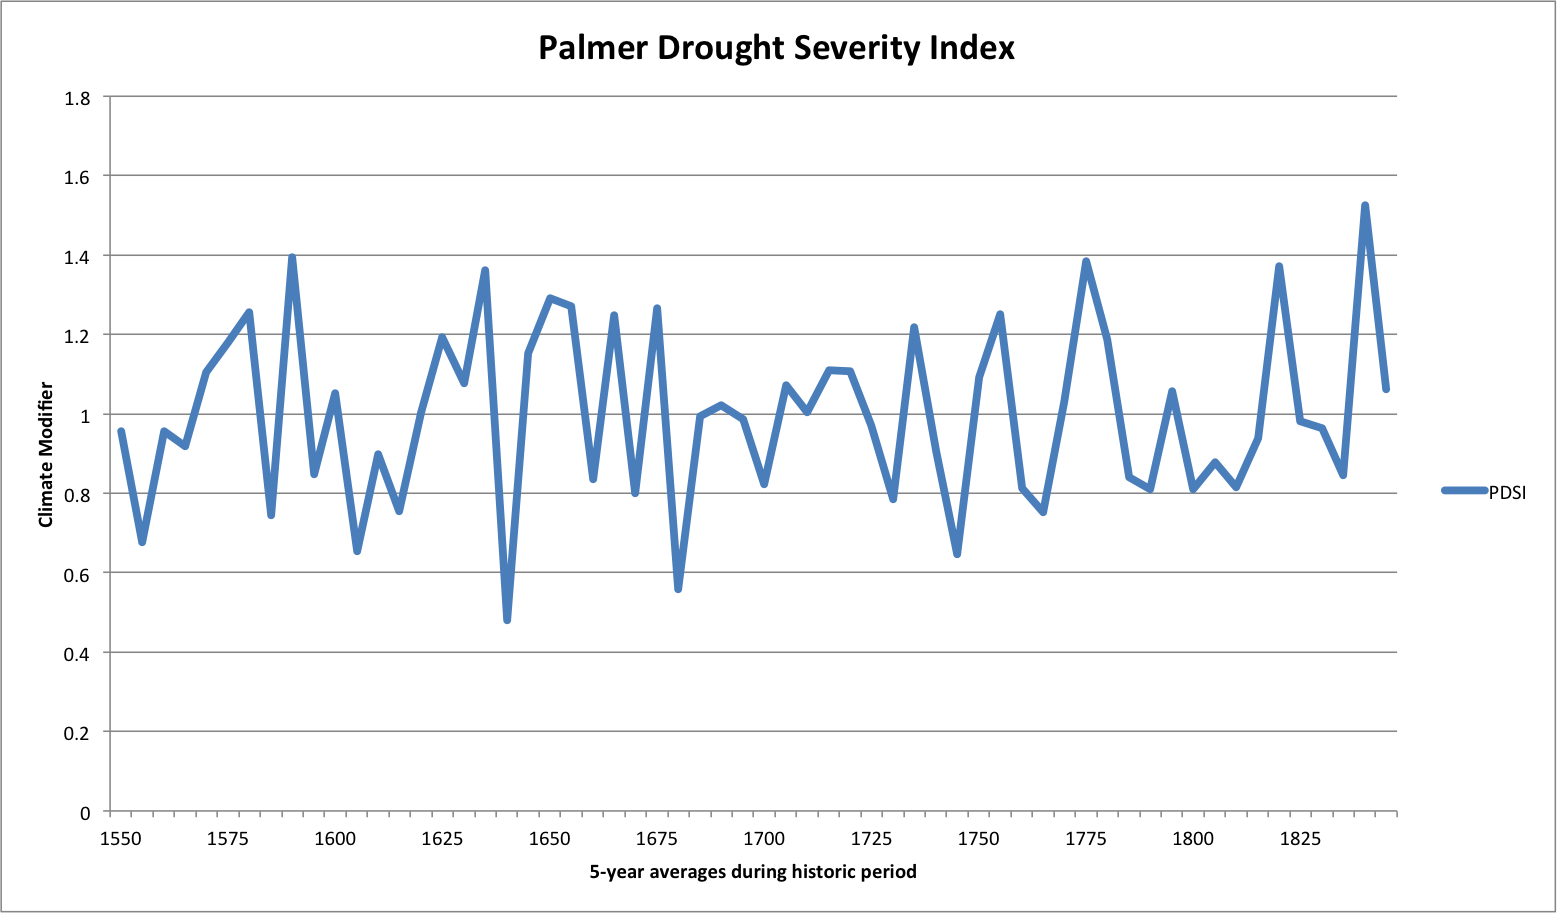
\includegraphics[height=0.3\textheight]{/Users/mmallek/Tahoe/Report2/images/pdsi.png}
\caption{Palmer Drought Severity Index, rescaled, inverted, and presented as a 5-year average for the ``historic'' period in this study (1550-1850).} 
\label{pdsi}
\end{figure}

%\medskip

%\noindent 
\item \emph{Susceptibility:} Cover and condition are both inputs to susceptibility. Cover modifies susceptibility via the ability to specify the influence of TPI on susceptibility (Table~\ref{covtpi}. The magnitude of this effect is estimated as a potential reduction in susceptibility of 30\% between the minimum and maximum TPI values used in the model. This is specified as part of a 4-parameter logistic function in which the left value is 0.7, right value is 1, slope is 1, and inflection point is 0.\todo{Are there typical symbols for these parameters we could use instead of right and left?} 

\begin{table}[htbp]
\small
\centering
\caption{Cover types whose susceptibility is modified by Topographic Position Index.}
\label{covtpi}
\begin{tabular}{ll}
\hline
\multicolumn{2}{c}{\textbf{Cover Types with TPI Adjustment}} \\
\hline
Grassland     									& Red Fir - Mesic   					\\
Lodgepole Pine    								& Red Fir - Ultramafic					\\
Mixed Evergreen - Mesic							& Red Fir - Xeric    					\\
Mixed Evergreen - Ultramafic     				& Sierran Mixed Conifer - Mesic    		\\
Mixed Evergreen - Xeric 						& Sierran Mixed Conifer - Ultramafic 	\\
Montane Riparian								& Sierran Mixed Conifer - Xeric 		\\
Oak Woodland 									& Western White Pine					\\
Oak-Conifer Forest and Woodland 				& Yellow Pine 							\\
Oak-Conifer Forest and Woodland - Ultramafic 	&										\\
\hline
\end{tabular}

\end{table}

Condition class further modifies susceptibility. We use the Weibull cumulative distribution function and specify a scale parameter $\lambda$ (mean return interval), shape parameter $k$, and the reset point for the function (\emph{age since high mortality disturbance} or \emph{age since any disturbance}). The mean return interval for the condition class is used as a calibration parameter and was initially set as equal to the values provided in analogous LandFire Biophysical Setting types.\todo{cite} Some modifications were made based on consultation with Forest Service staff. All mean return intervals within a cover type are modified as a group and kept relative to one another even as the magnitude of the return intervals is adjusted. We set $k=3$ for all cover types and condition classes. We selected between ``age since high mortality disturbance'' and ``age since any disturbance'' based on whether wildfires in that cover type are climate-driven (in which case we select the former) or fuels-driven (in which case we select the latter) (Figure~\ref{howdriven}). A detailed description of the specific parameters chosen is available \todo{in some sort of appendix type file, or perhaps in cover type description doc?}.

\begin{table}[htbp]
\small
\centering
\caption{Cover types sorted by whether wildfire disturbance in them is characterized by fuels present or overarching climatic conditions. If the likelihood of wildfire depends on the accumulation of fuels, the value of $x$ (``time since'') reverts to 0 after any disturbance. If the likelihood of wildfire depends primarily on climate and weather conditions, the value of $x$ reverts to 0 only after a high mortality disturbance.}
\label{howdriven}
\begin{tabular}{ll}
\hline
\textbf{Fuel-Driven Cover Types} 				& \textbf{Climate-Driven Cover Types}	\\
\hline
Curl-leaf Mountain Mahogany 					& Agriculture   						\\
Grassland     									& Big Sagebrush 						\\
Lodgepole Pine    								& Black and Low Sagebrush				\\
Meadow											& Lodgepole Pine with Aspen 			\\
Mixed Evergreen - Mesic							& Montane Riparian						\\
Mixed Evergreen - Ultramafic     				& Red Fir with Aspen   					\\
Mixed Evergreen - Xeric 						& Red Fir - Mesic    					\\
Oak Woodland 									& Red Fir - Ultramafic 					\\
Oak-Conifer Forest and Woodland 				& Red Fir - Xeric 						\\ 	
Oak-Conifer Forest and Woodland - Ultramafic 	& Subalpine Conifer 					\\
Sierran Mixed Conifer - Ultramafic 				& Subalpine Conifer with Aspen 			\\
Sierran Mixed Conifer - Xeric 					& Sierran Mixed Conifer with Aspen 		\\
Urban 											& Sierran Mixed Conifer - Mesic 		\\
Yellow Pine 									& Western White Pine 					\\
												& Yellow Pine with Aspen 				\\
\hline
\end{tabular}
\end{table}


%\medskip

%\noindent 
\item \emph{Initiation:} In \textsc{RMLands}, parameters for initiation are used as calibration parameters. The probability of wildfire initiation is a function of its susceptibility to wildfire and the climate modifier value for that timestep, and is applied at the cell level. The ignition calibration coefficient refers to the number of ignitions per 100,000 ha per year. For the HRV simulation, we set this coefficient at 38. We applied the coefficient evenly across the landscape based on local expert knowledge of lighting strike locations in the area (Alan Doerr and Marilyn Tierney, personal communication). Fires may be initiated anywhere within the project area or the 10 km buffer around it. The total area cover within that boundary is 409,410.7 ha, so up to 777 fire starts were possible during each timestep in our simulation (not all potential ignitions result in fire). Climate also influences initiation.

%\medskip

%\noindent 
\item \emph{Spread:} The probability of fire spread in \textsc{RMLands} is a function of climate, susceptibility to wildfire, potential wildfire size, wind, spotting, relative elevation, and presence of streams. The first two are described above. The disturbance size distribution that regulates potential fire size was created by analyzing the size distribution of all mapped fires in the Northern Sierra CalVeg mapping zone and west of the Sierran crest, available from the Forest Service and the California Department of Forestry and Fire Protection, which goes back to approximately 1900. 

Wind is incorporated in two parts. First, a prevailing wind direction for the fire is selected probabilistically from the eight cardinal directions. To compute the wind distribution values, we first consulted local experts to determine the dates of fire season (May 15 to October 15) and burning period times (1000 hours to 1800 hours). We then downloaded all available historic wind direction data from 6 local weather stations (Rice Canyon, Saddleback, Downieville, White Cloud, Emigrant Gap, and Blue Canyon, Figure~\ref{weather}). Data from all weather stations was weighted equally. After the wind direction is selected, fires are able to grow in all directions, but are relatively more likely to spread with wind than against it. We parameterized the influence of \emph{relative wind} as a reduction in spread likelihood. Thus, spread in the same direction as wind has a neutral effect, spread at $\ang{45}$ angles is reduced by 30\%, spread at $\ang{90}$  angles is reduced by 70\%, spread at $\ang{135}$ angles is reduced by 90\%, and spread opposite the prevailing wind direction is reduced by 95\%. 

\begin{figure}[htbp]
\centering
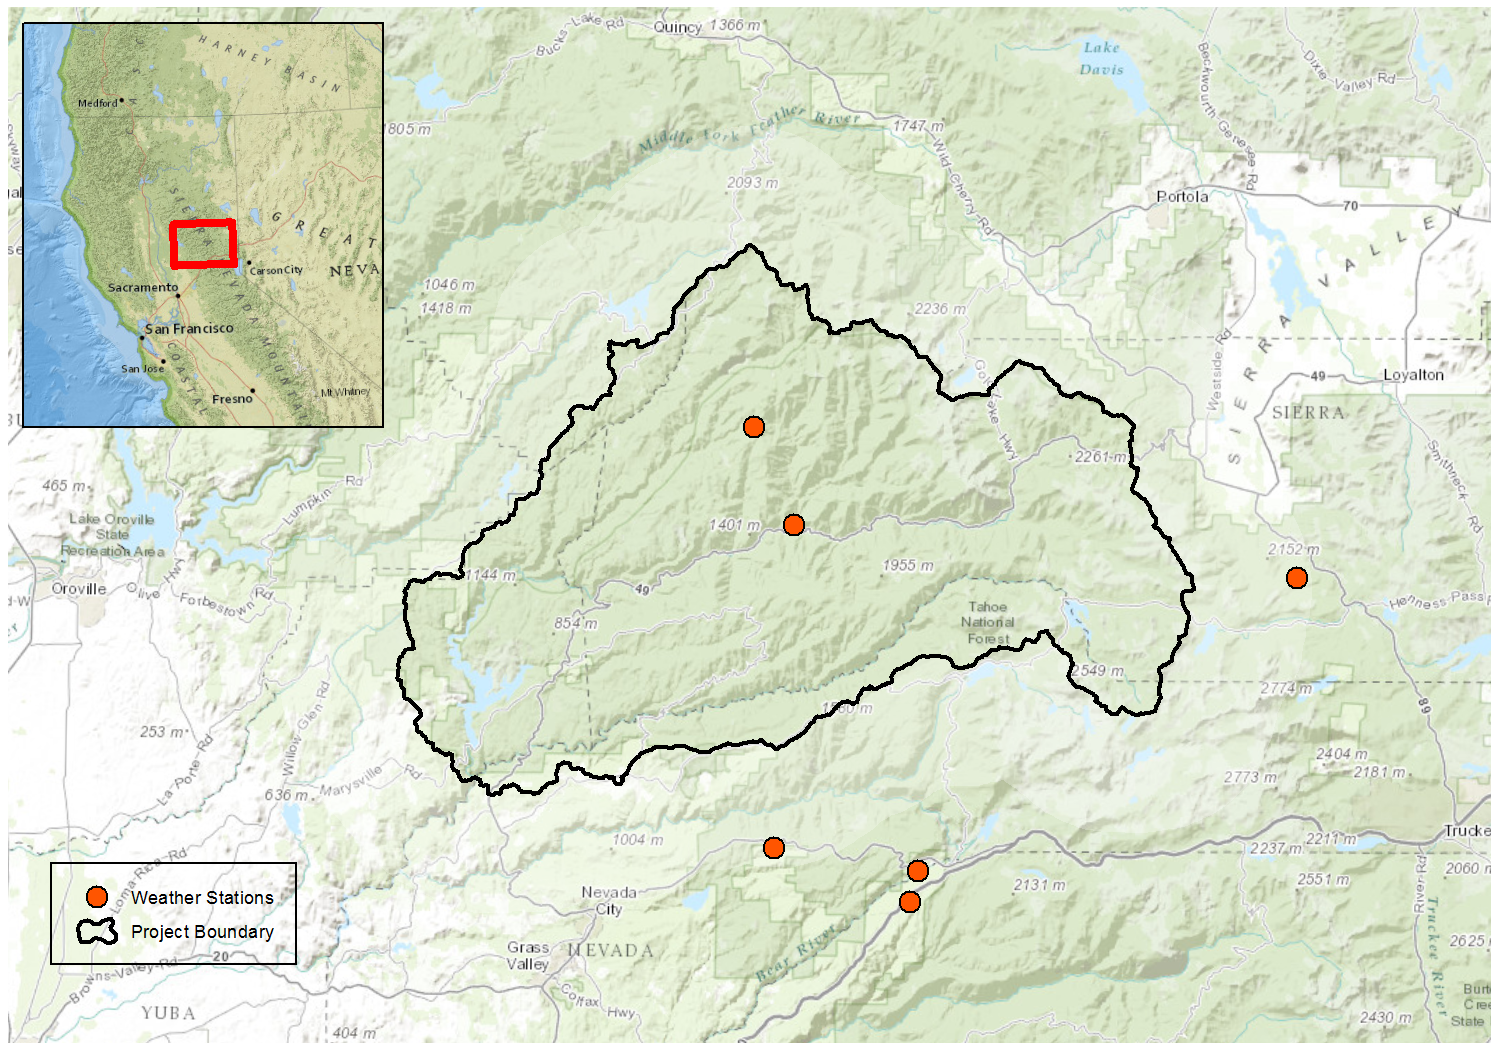
\includegraphics[width=0.8\textwidth]{/Users/mmallek/Tahoe/Report2/images/weather.png}
\caption{Weather stations used to inform wind direction parameters.}
\label{weather}
\end{figure}

Relative elevation also modifies spreading potential. We parameterized the model such that spread downhill is extremely unlikely. Spotting and the extent to which streams act as barriers to spread are affected by the fire size. As fires become larger, their probability of spotting and spotting distance increases. Similarly, streams function as a barrier to smaller fires, but large fires are able to spread past streams regardless of size. This decision is based on the idea that large fires are more influenced by wind and climatic conditions. Stream size does impact smaller fires; the largest streams and rivers are usually an effective barrier to smaller fires, although even fairly small fires often spread past intermittent and small perennial streams. 

For complete precise parameterization of the model, see \todo{Where would this go? Screenshots or table?}


\item \emph{Mortality:} Cover and condition are both inputs to mortality. The effect of topographic position is tied to cover: the mortality of certain cover types (Table~\ref{covtpi}) is affected by cover. The magnitude of this effect is estimated as a potential reduction in mortality of 30\% between the minimum and maximum TPI values used in the model. This is specified as part of a 4-parameter logistic function in which the left value is 0.7, right value is 1, slope is 1, and inflection point is 0. \todo{same issue - would be better to state greek letters instead of right/left.}

\begin{table}[htbp]
\small
\centering
\caption{Cover types whose mortality is modified by Topographic Position Index.}
\begin{tabular}{ll}
\hline
\multicolumn{2}{c}{\textbf{Cover Types with TPI Adjustment}} \\
\hline
Grassland     									& Red Fir - Mesic   					\\
Lodgepole Pine    								& Red Fir - Ultramafic					\\
Mixed Evergreen - Mesic							& Red Fir - Xeric    					\\
Mixed Evergreen - Ultramafic     				& Sierran Mixed Conifer - Mesic    		\\
Mixed Evergreen - Xeric 						& Sierran Mixed Conifer - Ultramafic 	\\
Montane Riparian								& Sierran Mixed Conifer - Xeric 		\\
Oak Woodland 									& Western White Pine					\\
Oak-Conifer Forest and Woodland 				& Yellow Pine 							\\
Oak-Conifer Forest and Woodland - Ultramafic 	&										\\
\hline
\end{tabular}
\end{table}

Condition class further modifies mortality. We extracted the likelihood of mortality from the VDDT models built during the LandFire project. However, our accounting method differs slightly. VDDT characterizes fire severity (e.g. mixed) independently from a particular outcome (e.g. resetting to early seral conditions). We do not include ``mixed severity'' fire in our model. Instead, we characterize fire dichotomously, based on their outcomes: fires are either high mortality or low mortality events. We define low mortality fires are those in which less than 70\% of overstory trees are killed, while high mortality fires are those in which more that 70\% of overstory trees are killed. 

To interpret the VDDT models, we analyzed not only the fire type (replacement, mixed, or surface), but also the change in \emph{condition} that occurred as a consequence of that fire. I classified the probabilities specified by the VDDT model as associated with either high or low mortality fires. High mortality fires are those that result in conversion to early seral (regardless of whether they are called ``replacement'' or ``mixed''). All other fires are considered low mortality. The probability of a high mortality outcome from fire was calculated by dividing the summed probabilities of high mortality fires as defined above by the summed probabilities of all fires. As an example, these probabilities for Sierran Mixed Conifer - Mesic are provided in Table~\ref{smcm_fri_phm} (Subsection~\ref{subsec:hrvmodelparam}).

\end{itemize}
%\end{adjustwidth}

\subsection{Model Calibration}
Calibrating the model was done by manipulating the ignition calibration coefficient and the relative magnitude of the scale parameter (mean fire return interval) $\lambda$ in the Weibull cumulative distribution function under Susceptibility. We first manipulated the ignition calibration coefficient and reran the simulation until the output cover type rotation values were in a range near their target. We then modified the fire return interval values as groups of condition classes under a given cover type to achieve our target rotations. For example, the target rotation for Sierran Mixed Conifer - Mesic was 29 years. As part of calibration, we adjusted the input condition class-based mean fire return interval up or down, eventually arriving at an increase by a factor of 3 from the original VDDT values. That is, each scale parameter value was multiplied by 3 in order to modify the susceptibility of Sierran Mixed Conifer - Mesic to fire without changing the relative susceptibility among Sierran Mixed Conifer - Mesic condition classes. We came very close to achieving our target cover type rotation values through several iterations of this method, and the final step was to make a final small modification to the ignitition calibration coefficient.

\subsection{Model Execution}
During the calibration phase of the model, a typical simulation would be three runs of 200 timesteps each. The equilibration period of 40 timesteps was chosen based on visual analysis of the disturbed area and rotation plots from the combined runs. Once calibration was complete, we conducted one 500 timestep-long run in order to capture multiple disturbance and succession cycles across the most common cover types. Each timestep represents five years. The five-year timestep was chosen based on the short fire return intervals recorded from dendrochronology analysis in the literature and our desire to capture these very short return intervals in the simulation.

\subsection{Data Analysis}
\label{subsec:dataanalysis}

\paragraph{Disturbance Regime} We quantified the following overall temporal and spatial characteristics of the wildfire disturbance regime:
\begin{itemize}
	\item \emph{Disturbed Area:} We calculate disturbed area for each timestep, divided into low mortality and high mortality disturbance, and summed to produce an ``any mortality'' statistic. We summarize the results for minimum, maximum, mean, and median area disturbed as a proportion of the total area eligible for disturbance for the full simulation excluding the equilibration period (460 timesteps, or 2300 years). We also present maps of the landscape illustrating the minimum, maximum, and median area burned during the simulation, and a 4-timestep sequence illustrating a time series of wildfire disturbance. Finally, we present the distribution of wildfire extents during the simulation, excluding the equilibration period, as a barplot.\todo{make sure these are in the results section}
	\item \emph{Disturbance Frequency:} We calcuate the number of years between disturbances exceeding a particular threshold in total disturbed area. We report the frequency of timesteps during which at least 10\%, 25\%, or 50\% of the landscape experienced wildfire.
	\item \emph{Climate Effect:} Climate interacts with several components of the model. We present plots illustrating the change in the climate parameter by timesteps concurrently with the area disturbed per timestep. It is not practical to further illustrate its effect everywhere, and in some cases its influence is not easily separated from the other inputs to the model. \todo{be sure to make this plot} 
	\item \emph{Rotation Period:} We calculate the rotation period---the number of years required to burn an area equivalent ot the total eligible area---for each cover type within the project area. It is based on the census, not a sample, of the population of cells within the project area, and is therefore equivalent to the cell-specific grand mean return interval for a given cover type across the landscape. We report the rotation values for low mortality fire, high mortality fire, and any fire. We also report this data for the full landscape.
	\item \emph{Return Interval:} We summarize the cell-specific population mean return interval---the average number of years between disturbances at a single cell---and present it as the distribution of the percentage of eligible cells that experienced each possible mean return interval. We present histograms for low mortality fire, high mortality fire, and any fire, along with their median values. As with the rotation period, this method uses the census, not a sample, of the population of cells within the project area, and is therefore equivalent to the cell-specific grant mean return interval for a given cover type across the landscape. We also report this data for the full landscape. Finally, we present this result spatially as a map showing the population fire return interval for the full landscape and for our nine focal cover types.
\end{itemize}

\paragraph{Vegetation Response} 

\begin{itemize}
\item \emph{Landscape Composition:} We quantified the distribution and dynamics of landscape composition by cover type. For our single 2500 year simulation (with 200 year equilibration period), we summarize the results in a table and in stacked bar plots. For the tabular results, we present the mean, median, minimum, maximum, 5th, 25th, 75th and 95th percentiles of the distribution. We compared the current landscape condition (i.e., proportion of cover type in each condition class) to this simulated historic range of variability to determine whether the current landscape deviates, and to what degree, from the HRV. In the body of this report we present results for the nine focal cover types that occur over at least 1000 ha on the project landscape; others are available \todo{in an appendix? not at all?}. We visualize the proportion of the total area of a given cover type occuring as each condition class, for each timestep in the model. In addition, we show a simple plot of current conditions, allowing a visual comparison between current conditions and the historic range of variability in the distribution of the condition classes.

\item \emph{Landscape Structure and Patterns:} We used \textsc{Fragstats} \todo{cite v4.2} to compute several landscape-level and class-level metrics that summarize landscape structure over the course of the simulation. We present the results in a series of tables and figures. The descriptions below are intended as a general introduction to the \textsc{Fragstats} metrics; for a much more detailed and mathematical description of all \textsc{Fragstats} metrics, see the \href{http://www.umass.edu/landeco/research/fragstats/documents/fragstats.help.4.2.pdf}{documentation}. Each metric is computed on the study area for a single timestep and the results are displayed in tabular format by quantiles and in graphical format with line graphs.

	\begin{enumerate}
		\item Percentage of Landscape (PLAND)\\
		\emph{Landscape}-level: not computed\\
		\emph{Class}-level: the percentage of the landscape comprised of a particular patch type\\
		
		%\item Core Area Percentage of Landscape (CPLAND)\\
		%\emph{Landscape}-level: not computed\\
		%\emph{Class}-level: the sum of all core areas in a given patch type divided by the total landscape area; reported as a percentage%\\

		\item Patch Density (PD)\\
		\emph{Landscape}-level: number of patches of all cover types and condition classes divided by the total landscape area for one timestep\\
		\emph{Class}-level: number of patches of a give cover type and condition class divided by the total area occupied by that cover-condition type\\
		
		\item Edge Density (ED) \\
		\label{item:ED}
		\emph{Landscape}-level: the sum of the lengths of all edge segments divided by the total landscape area\\	
		\emph{Class}-level: the sum of the lengths of all edge segments for a given patch type divided by the total area occuring as that patch type\\

		\item Total Edge Contrast Index (TECI) \\
		\label{item:TECI}
		\emph{Note}: Contrast refers to the relative difference among patch types. For example, mature forest next to young forest might have a lower-contrast edge than mature forest adjacent to open field. A contrast weight is assigned to each possible pair of condition classes before running \textsc{Fragstats}. 	\\
		\emph{Landscape}-level: the sum of the lengths of all edge segments in the landscape multiplied by the appropriate contrast weight, divided by the total length of edge in the landscape\\
		\emph{Class}-level: the sum of the products of the lengths of all edge segments for a given patch type and the appropriate contrast weight, divided by the sum of the lengths of all edge segments for a given patch type \\
		
		%\item Mean Area (AREA\_MN)\\
		%\emph{Landscape}-level:  mean patch area across all cover types and condition classes\\
		%\emph{Class}-level:  mean patch area across all condition classes for a given cover type\\
		
		\item Area-Weighted Mean Area (AREA\_AM)\\
		\emph{Note}: Area-weighted metrics are used to reduce the influence of the many isolated, single-pixel ``patches'' that are an artifact of the model and do not represent true ecological processes. They reflect the mean metric value for a cell selected at random on the landscape. 	\\
		\emph{Landscape}-level: area-weighted mean patch area across all cover types and condition classes \\
		\emph{Class}-level: area-weighted mean patch area across all condition classes for a given cover type. \\
		
		\item Area-Weighted Mean Radius of Gyration (GYRATE\_AM)\\
		\emph{Landscape}-level: measure of the area-weighted mean length across the landscape a patch extends its reach; in other words, calculate the shortest path between every possible pair of cells within a patch and take the longest of this set, then take the average of these ``longest'' paths for every patch on the landscape\\
		\emph{Class}-level: for a given cover type and condition class, the area-weighted mean average length of a patch on the landscape\\
		
		%\item Mean Shape (SHAPE\_MN) measures the complexity of patch shape compared to a square of the same size\\
		%\emph{Landscape}-level: length of patch perimeter for all patch type on the landscape divided by the area of the landscape, %adjusted to a square standard, and averaged across all patch types\\
		%\emph{Class}-level: length of patch perimeter for each patch type on the landscape divided by the square root of the area in that patch type, adjusted to a square standard \\
		
		\item Area-Weighted Mean Shape (SHAPE\_AM)\\
		\emph{Note}: the theoretical idea behind Shape is to compare a patch to the simplest shape, a square 		\\
		\emph{Landscape}-level: length of patch perimeter for all patch types on the landscape divided by the total landscapearea, adjusted to a square standard, and converted to an area-weighted mean across all patch types \\
		\emph{Class}-level: length of patch perimeter for each patch type on the landscape divided by the square root of the area in that patch type, adjusted to a square standard\\
		
		%\item Mean Core Area (CORE\_MN)\\
		%\emph{Landscape}-level: total core area on the landscape, divided by landscape area\\
		%\emph{Class}-level: total core area within each patch type on the landscape, divided by the total area in the same patch type\\
		
		\item Area-Weighted Mean Core Area (CORE\_AM)\\
		\emph{Note}: Core area is defined as the area within a patch beyond some specified depth-of-edge influence (i.e., edge distance) or buffer width and is important for organisms who specialize in patch interiors 	\\
		\emph{Landscape}-level: total core area within each patch on the landscape, divided by the total landscape area in the same patch type	\\
		\emph{Class}-level: total core area within a given patch type on the landscape, divided by the total area in the same patch type	\\
		
		\item Area-Weighted Mean Core Area Index (CAI\_AM)\\
		\emph{Landscape}-level: core area for the landscape as a percentage of total landscape area \\
		%core area of a patch divided by total area of a patch, multiplied by the area of that patch divided by the area of the landscape; reported as a percentage	\\
		\emph{Class}-level: core area for a given patch type as a percentage of a total area in that patch type
		%core area of a patch divided by total area of a patch, multiplied by the area of that patch divided by the total area of that patch type; reported as a percentage	\\
		
		\item Mean Similarity Index (SIMI\_MN)\\
		\emph{Note}: Similarity distinguishes sparse distributions of small and insular habitat patches from configurations where the habitat forms a complex cluster of larger, hospitable (i.e., similar) patches. A similiarity value is assigned to each possible pair of condition classes before running \textsc{Fragstats}. 	\\
		\emph{Landscape}-level: the average of the similarity value for each patch on the landscape \\
		%the average sum over all neighboring patches with edges within a specified distance of the focal patch, of: neighboring patch area times a similarity coefficient between the focal patch type and the class of the neighboring patch, divided by the nearest edge-to-edge distance squared between the focal patch and the neighboring patch	\\
		\emph{Class}-level: the average of the similarity value for each patch within a given patch type \\
		%the average sum over all neighboring patches with edges within a specified distance of the focal patch, of: neighboring patch area times a similarity coefficient between the focal patch type and the class of the neighboring patch, divided by the nearest edge-to-edge distance squared between the focal patch and the neighboring patch; reported for each patch type separately	\\
		
		\item Contrast-Weighted Edge Density (CWED)\\
		\emph{Note}: This metric is intended to highlight the functional importance of edge	\\
		\emph{Landscape}-level: the sum of the lengths of all edge segments divided by the total landscape area (Edge Density, metric~\ref{item:ED}), multiplied by a contrast weight (metric~\ref{item:TECI})
		\emph{Class}-level: the sum of the lengths of all edge segments for a given patch type divided by the total landscape area, multiplied by the appropriate contrast weight (metric~\ref{item:TECI})  	\\

		\item Contagion (CONTAG)\\
		\emph{Landscape}-level: a cell-based (as opposed to patch-based) metric that measures the likelihood of a given cell belonging to the same patch type as a randomly chosen adjacent cell and is a common measure of both aggregation and dispersion 	\\
		%1 minus the sum of the proportional abundance of each patch type multiplied by the proportion of adjacencies between cells of that patch type and another patch type, multiplied by the logarithm of the same quantity, summed over each unique adjacency type and each patch type; divided by 2 times the logarithm of the number of patch types; reported as a percent; inversely related to edge density\\
		\emph{Class}-level: not computed \\ 	
		
		\todo{not sure how to fix Clumpy explanation}		
		\item Clumpiness Index (CLUMPY)\\
		\emph{Landscape}-level: not computed  	\\
		\emph{Class}-level: similar conceptually (though not mathematically) to Contagion, the Clumpiness Index indicates how fragmented or aggregated the cells of a given patch type are; values range from -1 (completely dispersed) to 1 (maximally clumped), with 0 representing a completely random configuration 	\\
		%the proportional deviation of the proportion of like adjacencies involving the corresponding class from that expected under a spatially random distribution. If the proportion of like adjacencies ($G_i$) is $\geq$ the proportion of the landscape comprised of the focal class ($P_i$), then $\text{CLUMPY} = \frac{G_i - P_i}{1 - P_i}$. If $G_i < P_i \text{and} P_i \geq 0.5, \text{then CLUMPY} = \frac{G_i - Pi}{1 - P_i}$. If $G_i < Pi \text{and} P_i < 0.5, \text{then CLUMPY} = \frac{P_i - G_i}{-P_i}$.	\\
		
		\item Interspersion and Juxtaposition Index (IJI) \\
		\emph{Landscape}-level: a patch-based metric that represents the observed level of interspersion as a percentage of the maximum possible given the total number of patch types; based on the total length of edge in the landscape 	\\
		%similar to Contagion, but patch-based rather than cell-based; ranges from 0 (uneven configuration of patches - low interspersion and juxtaposition) to 100 (maximally evenly interspersed or juxtaposed patches) 	\\
		%-1 times the sum of the length of each unique edge type divided by the total landscape edge, multiple by the logarithm of the same quantity, summed over each unique edge type;  divided by the logarithm of the number of patch types times the number of patch types minus 1 divided by 2 	\\
		\emph{Class}-level: a patch-based metric that represents the observed level of interspersion as a percentage of the maximum possible given the total number of patch types, based on length of edge between the focal patch type and other patch types 	\\
		%similar to the Clumpiness index, but patch-based rather than cell-based; ranges from 0 (uneven configuration of patches - low interspersion and juxtaposition) to 100 (maximally evenly interspersed or juxtaposed patches) based on length of edge between the focal patch type and other patch types 	\\
		%-1 times the sum of the length of each unique edge type involving the corresponding patch type divided by the total length of edge involving the same type, multiplied by the logarithm of the same quantity, summed over each unique edge type; divided by the logarithm of the number of patch types minus 1; reported as a percentage	\\
		
		\item Patch Richness (PR)\\
		\emph{Landscape}-level: the number of patch types present in the landscape	\\
		\emph{Class}-level: not computed \\
		
		\item Simpson's Diversity Index (SIDI)\\
		\emph{Landscape}-level: the probability that any 2 pixels selected at random would be different patch types	\\
		\emph{Class}-level: not computed\\
		
		\item Simpson's Evenness Index (SIEI) \\
		\emph{Landscape}-level:  the observed level of diversity divided by the maximum possible diversity for a given patch richness 	\\
		\emph{Class}-level: not computed\\
		
		\item Aggregation Index (AI) - an area-weighted mean class aggregation index \\
		\emph{Landscape}-level: cell-based metric based on the ratio of the observed number of like adjacencies to the maximum possible number of like adjacencies; similar in interpretation to Contagion, but uses different statistical methods
		%the number of cells of the same cover and condition (patch type) adjecent to one another, multiplied by the proportion of the landscape comprised of that that patch type, summed over all classes; reported as a percentage	\\
		\emph{Class}-level: the number of cells of a given patch type adjacent to one another divided by the maximum possible number of like adjacencies for that patch type; similar in interpretation to the Clumpiness index, but uses different statistical methods	\\
	\end{enumerate}

\end{itemize}

%%%%%%%%%%%%%%%%%%%%%%%%%%%%%%%%%%%%%%
%%%%%%%%%%%%%%%%%%%%%%%%%%%%%%%%%%%%%%
%%%%%%%%%%%%%%%%%%%%%%%%%%%%%%%%%%%%%%
%%%%%%%%%%%%%%%%%%%%%%%%%%%%%%%%%%%%%%
%%%%%%%%%%%%%%%%%%%%%%%%%%%%%%%%%%%%%%
%%%%%%%%%%%%%%%%%%%%%%%%%%%%%%%%%%%%%%
%%%%%%%%%%%%%%%%%%%%%%%%%%%%%%%%%%%%%%
\section{Future Management Scenarios}

\subsection{Input Layers}

\subsubsection{Roads} 
Roads represents all transportation corridors classified as small, medium or large based on road size and/or intensity of use. It is only used during future scenarios simulations. Roads is a \emph{static} grid; cell values remain constant over time. Note, roads can also be integrated into the cover type classification scheme and represented in the cover grid depending on the application. However, in the current version of \textsc{RMLands} it is necessary to include a separate roads grid regardless of whether road features are integrated into the cover grid or not.

In this application, the roads layer was created from a line coverage containing transportation data, including an attribute for roads size or order, by converting to a grid based on the roads size attribute. Roads are used to affect disturbance spread in \textsc{RMLands}; i.e., roads function as an impediment to spread. We employed the orthogonal neighbor rule when converting a line to a raster of like-valued cells. That is, the final grid contains stream cells that connect along a cell side, as opposed to diagonally. This is required because diagonal neighbors, while touching, will not provide an impediment to disturbance spread (which happens diagonally as well as orthogonally). In addition, road proximity - which is derived from roads - can be used to constrain and/or prioritize areas for vegetation treatments. 

It is extremely important that the rasterization process employ the orthogonal neighbor rule when converting a line to a string of like-valued cells. Specifically, the final grid should contain road cells that connect along a cell side (i.e., orthogonally) as opposed to diagonally. The diagonal neighbors, while touching, will not provide an impediment to disturbance spread (which happens diagonally as well as orthogonally). In addition, roads do not have to be in a contiguous network (i.e., no breaks in the roads) as long as the implications in terms of disturbance spread and/or logical treatment boundaries are understood and accepted. 


\subsubsection{Vegetation Treatment Layers}

When simulating future scenarios, \textsc{RMLands} accepts parameterization for vegetation treatments across the landscape. We identified four classes of vegetation treatments, and created a \emph{static suitability layer} for each. These treatment priority layers were created through a series of geoprocessing steps that included developing several input layers, assigning probabilities to each, and computing the geometric mean of the layer set. We incorporated the following layers into treatment priorities:
\begin{itemize}
	\item Wildland Urban Interface: composed of urban core, defense zone, and threat zone
	\item Goshawk and Spotted Owl Protected Activity Centers
	\item Slope
	\item Riparian Conservation Areas: 300 ft along each side of perennial streams, and 150 ft from each side of intermittent and ephemeral streams
	\item Topographic Position Index (rescaled according to a logistic function)
	\item Roadless areas
	\item Road Proximity: Euclidean distance from the closest road
\end{itemize}

\subsubsection{Compartments}

\subsubsection{Boundaries}


\begin{table}[ht]
\small
\centering
\caption{Values for individual input layers to treatment priority grids in \textsc{RMLands}. To create the grid for each treatment class (e.g. `Understory Mechanical'), the geometric mean of the 11 inputs was computed, allowing 0 values to be preserved. Each output grid is scaled from 0-1 and acts as a probability surface for the generation of treatment units in \textsc{RMLands}.}
\label{treatpri_table}
\begin{tabular}{@{}llllll@{}} 
    & \multicolumn{4}{c}{Treatment Priority Grids} &  \\ 
    \cmidrule(r){2-6}
    
    & \begin{tabular}[c]{@{}l@{}}Understory 	\\ 
    
    Mechanical\end{tabular}		& \begin{tabular}[c]{@{}l@{}}Prescribed \\ 
    
    Fire\end{tabular} 			& Thinning 	& \begin{tabular}[c]{@{}l@{}}Matrix Thin \\ \& Group Cut\end{tabular} 	& \begin{tabular}[c]{@{}l@{}}Methods/\\ Algorithm\end{tabular} \\ 
    \cmidrule(r){1-6}
	
	\multicolumn{1}{l}{WUI + PAC}  	& \multicolumn{1}{l}{0.6} 	& \multicolumn{1}{l}{0.6} 	& \multicolumn{1}{l}{0.4} 	& \multicolumn{1}{l}{0.2} 	& classified        \\ 
	
	\rowcolor[HTML]{EFEFEF} \multicolumn{1}{l}{nonWUI PAC} 	& \multicolumn{1}{l}{0}  	& \multicolumn{1}{l}{0.4} 	& \multicolumn{1}{l}{0}	& \multicolumn{1}{l}{0} 	& classified  	\\ 	
	
	\multicolumn{1}{l}{NonWUI, nonPAC} 	& \multicolumn{1}{l}{0.6} 	& \multicolumn{1}{l}{0.8} 	& \multicolumn{1}{l}{0.8} 	& \multicolumn{1}{l}{0.8} 	& classified  	\\ 

	\rowcolor[HTML]{EFEFEF} \multicolumn{1}{l}{\begin{tabular}[c]{@{}l@{}}WUI Threat Zone \\ excluding PAC\end{tabular}}     & \multicolumn{1}{l}{0.8}        & \multicolumn{1}{l}{0.8}        & \multicolumn{1}{l}{0.8}        & \multicolumn{1}{l}{0.8}        & classified        \\ 

	\multicolumn{1}{l}{\begin{tabular}[c]{@{}l@{}}WUI Defense Zone \\ excluding PAC\end{tabular}}    & \multicolumn{1}{l}{1}          & \multicolumn{1}{l}{1}          & \multicolumn{1}{l}{1}          & \multicolumn{1}{l}{1}          & classified        \\ 

	\rowcolor[HTML]{EFEFEF} \multicolumn{1}{l}{\begin{tabular}[c]{@{}l@{}}WUI Urban Core Zone \\ excluding PAC\end{tabular}} & \multicolumn{1}{l}{1}          & \multicolumn{1}{l}{1}          & \multicolumn{1}{l}{1}          & \multicolumn{1}{l}{1}          & classified        \\ 

	\multicolumn{1}{l}{Riparian}                          & \multicolumn{1}{l}{0}          & \multicolumn{1}{l}{0}          & \multicolumn{1}{l}{0}          & \multicolumn{1}{l}{0}          & classified        \\ 

	\rowcolor[HTML]{EFEFEF} \multicolumn{1}{l}{Slope}  	& \multicolumn{1}{l}{calculated} & \multicolumn{1}{l}{calculated} & \multicolumn{1}{l}{calculated} & \multicolumn{1}{l}{calculated} & logistic function \\ 

	\multicolumn{1}{l}{TPI}  	& \multicolumn{1}{l}{calculated} & \multicolumn{1}{l}{calculated} & \multicolumn{1}{l}{calculated} & \multicolumn{1}{l}{calculated} & linear 	\\ 	

	\rowcolor[HTML]{EFEFEF} \multicolumn{1}{l}{Road Proximity} 	& \multicolumn{1}{l}{calculated} & \multicolumn{1}{l}{calculated} & \multicolumn{1}{l}{calculated} & \multicolumn{1}{l}{calculated} & linear 	\\ 

	\multicolumn{1}{l}{Roadless} 	& 0 	& 0 	& 0  	 & 0 	 & 	\\ \cmidrule(r){1-6}
\end{tabular}
\end{table}

\begin{figure}
\centering
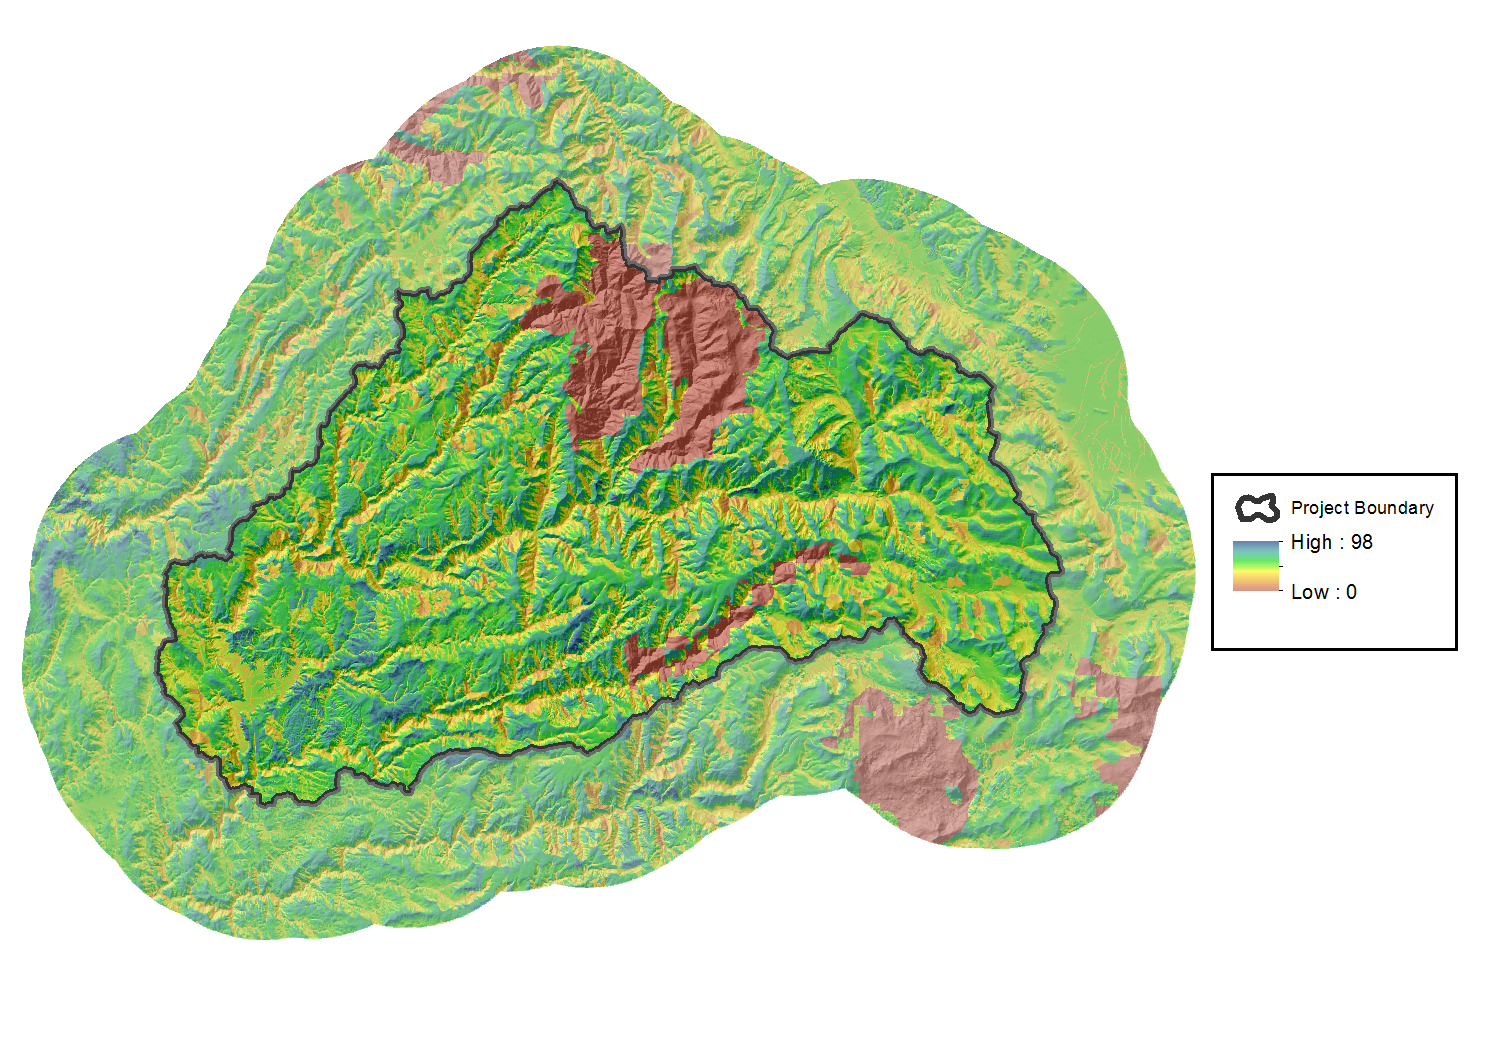
\includegraphics[height=0.4\textheight]{/Users/mmallek/Tahoe/Report2/images/treatpri_rxfire.png}
\caption{Treatment Priority grid for Prescribed Fire treatment class.} 
\label{treatpri_rxfire}
\end{figure}

\begin{figure}
\centering
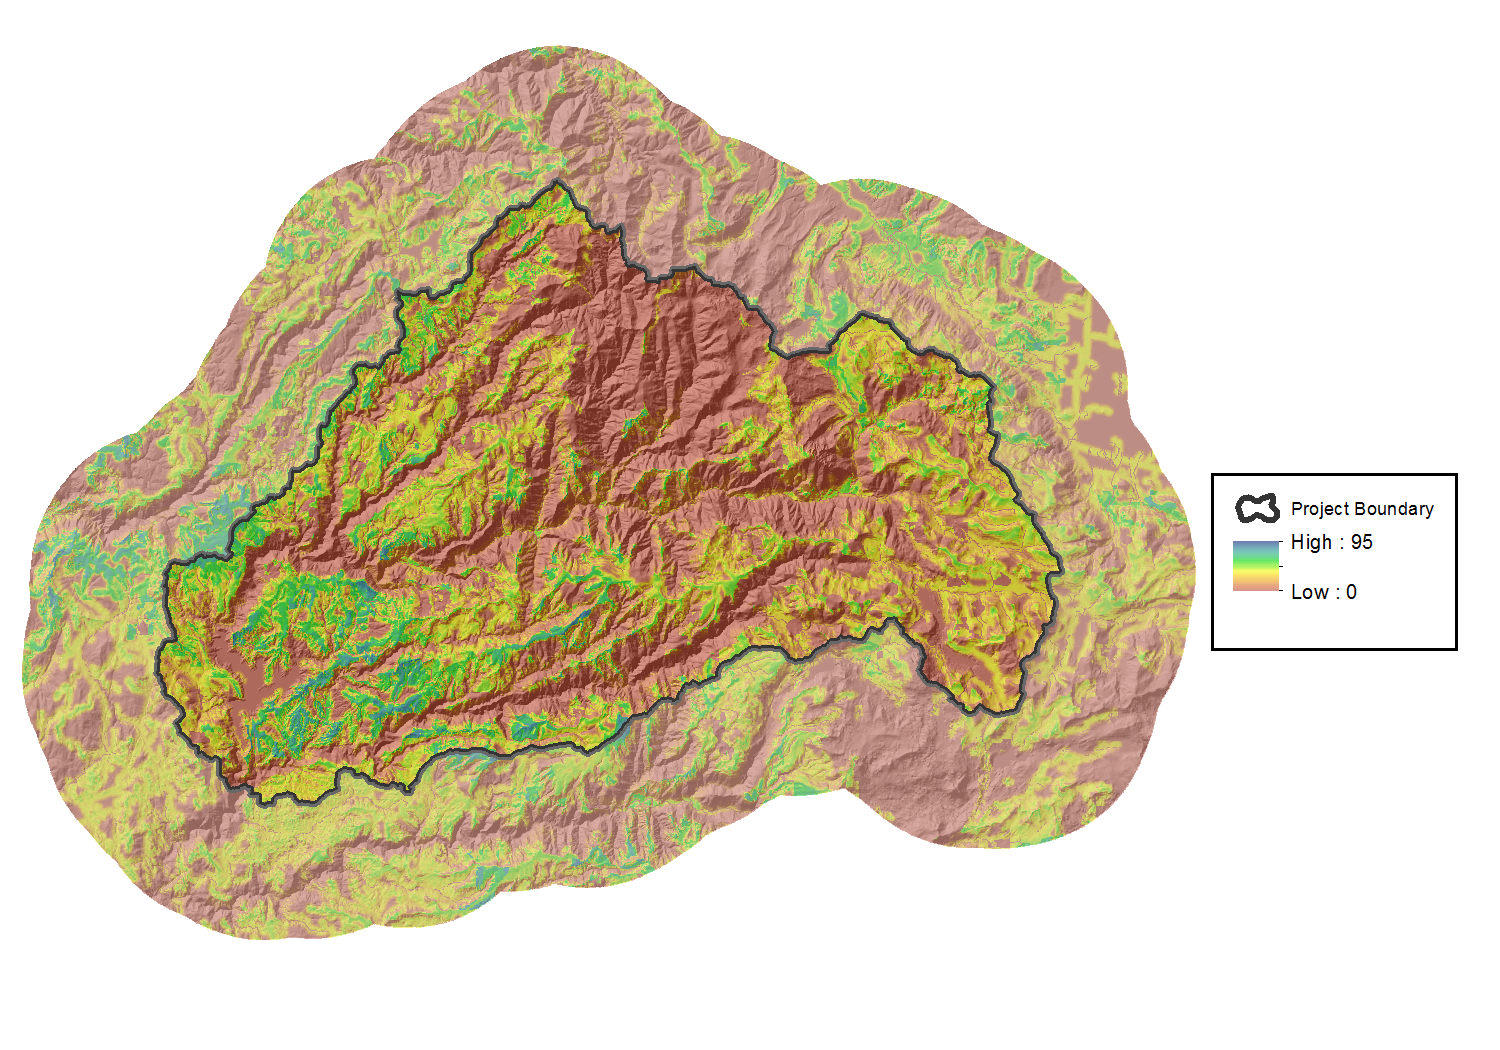
\includegraphics[height=0.4\textheight]{/Users/mmallek/Tahoe/Report2/images/treatpri_undermech.png}
\caption{Treatment Priority grid for Understory Mechanical treatment class.} 
\label{treatpri_undermech}
\end{figure}

\begin{figure}
\centering
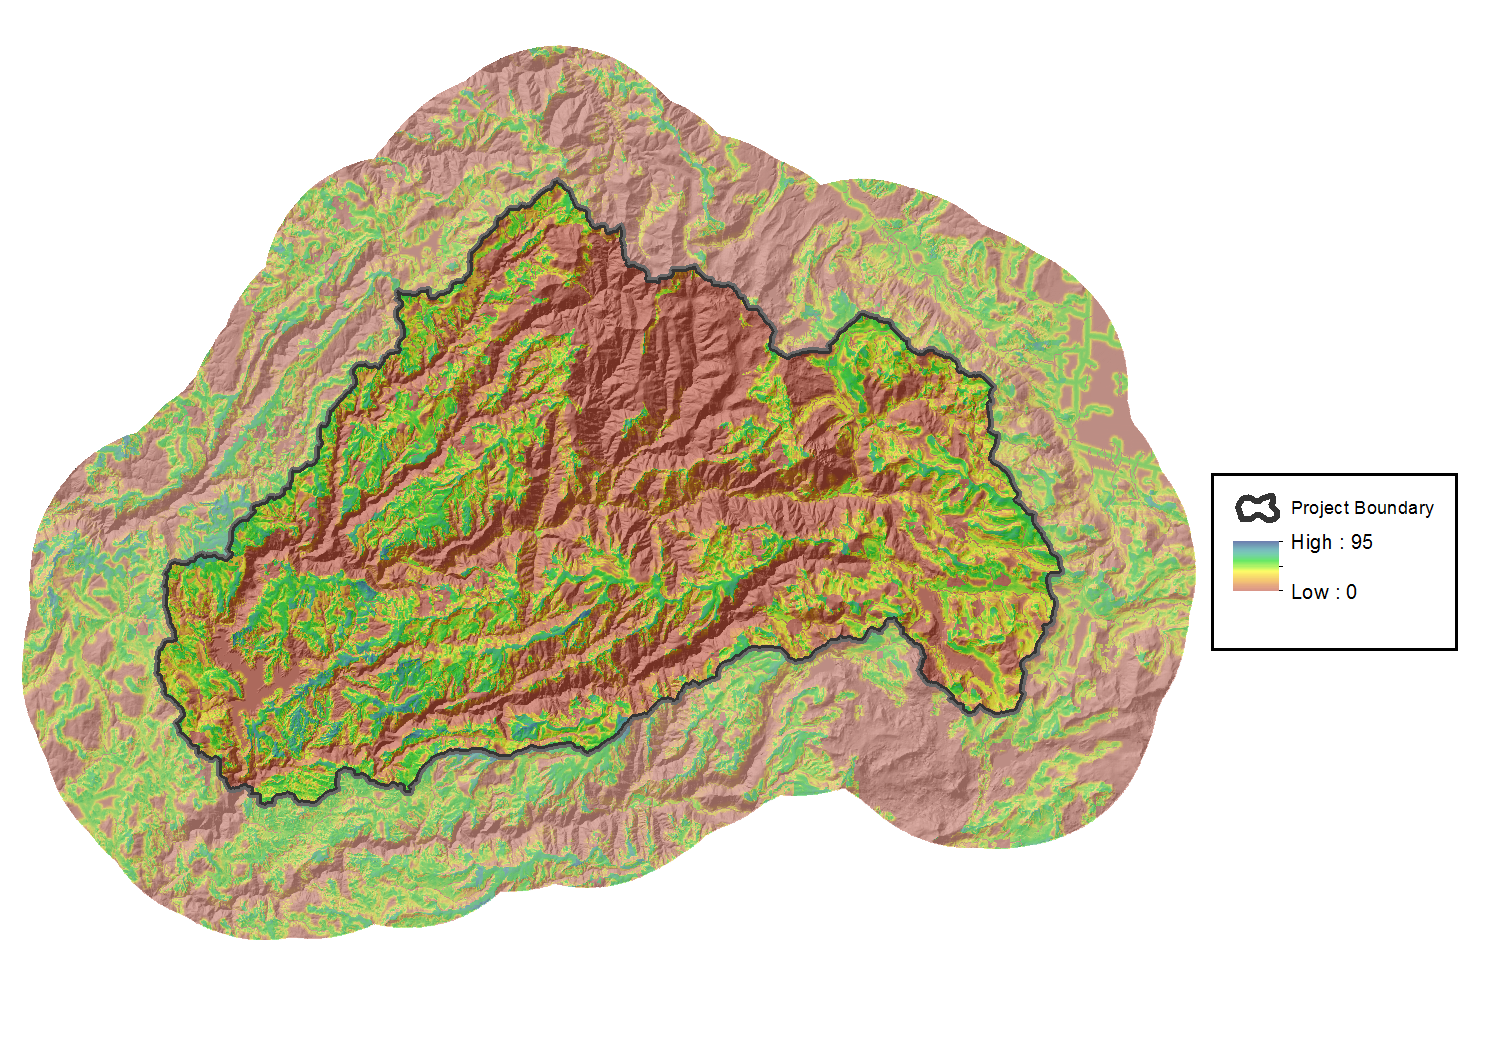
\includegraphics[height=0.4\textheight]{/Users/mmallek/Tahoe/Report2/images/treatpri_thin.png}
\caption{Treatment Priority grid for Thinning treatment class.} 
\label{treatpri_thin}
\end{figure}

\begin{figure}
\centering
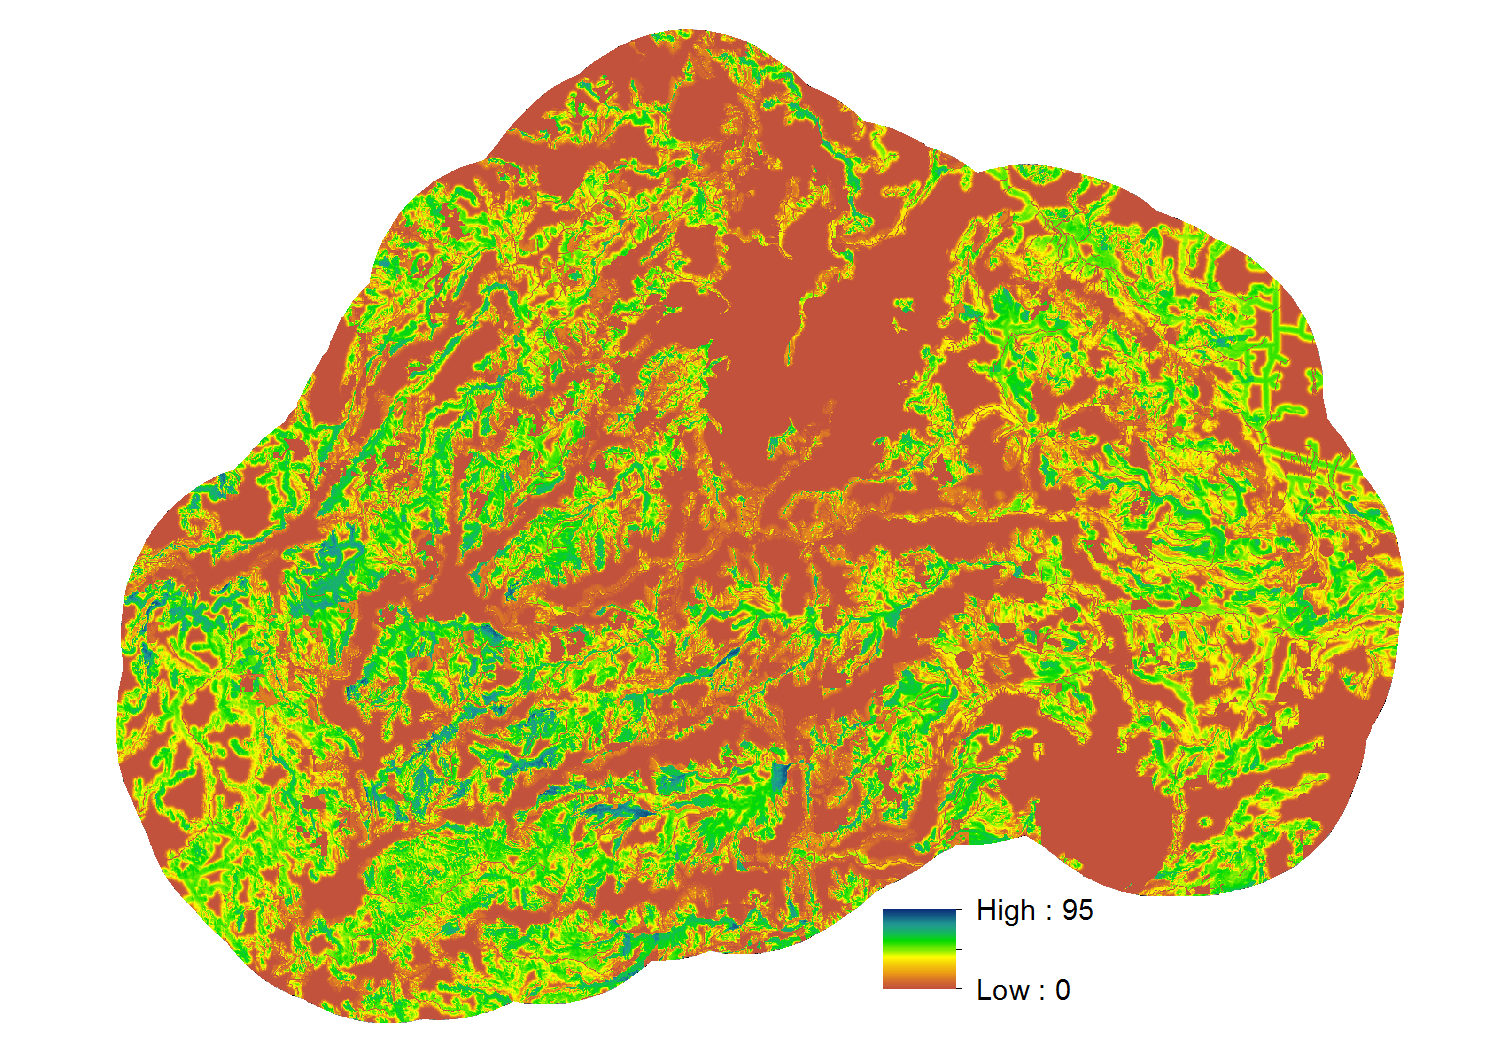
\includegraphics[height=0.4\textheight]{/Users/mmallek/Tahoe/Report2/images/treatpri_matgroup.png}
\caption{Treatment Priority grid for Matrix Thin \& Group Cut treatment class.} 
\label{treatpri_matgroup}
\end{figure}

\subsection{Model Parameterization}

\subsection{Model Calibration}

\subsection{Model Execution}

\subsection{Data Analysis}



 

\chapter{Results}

\section{Historic Range of Variability}

\subsection{Disturbance Regime}

This report focuses on the effects of wildfire as a natural disturbance; the impacts of other natural disturbances during the reference period were likely localized in time or space and therefore probably had far less impact on vegetation patterns over broad spatial and temporal scales than did fire.\todo{is this true?} In the sections below, we briefly describe the simulated disturbance regime (i.e., spatial extent and distribution, frequency and temporal variability). In this subsection, we refrain from describing variations among vegetation types. This will be accomplished in chapter~\ref{ch:covtype}. Finally, it is important to realize that while the information below is presented as ``results,'' it could have easily been presented in the methods section as ``model calibration.'' Key spatial and temporal aspects of the disturbance regime were evaluated during preliminary calibration runs, and we subsequently adjusted model parameters to effect desired changes. Thus, while the information presented below does in fact represent results (output) of the simulation, it also represents a set of targets used to calibrate the model (i.e., adjust model parameters to achieve desired results). While this may seem a bit circular, it was a necessary process for a complex model such as \textsc{RMLands}. Moreover, our real emphasis was on quantifying the vegetation patterns and dynamics resulting from these disturbance processes. 

\subsubsection{Disturbed Area}

% 174830 eligible hectares
% 181550 hectares in core
% check math using Wildfire_darea_trajectory.csv
Approximately 96\% of the landscape was eligible for wildfire disturbance (all cover types except Barren and Water)\footnote{In this section we report values based on percent of eligible landscape. There are 181,500 hectares in the core project area, and 174,830 remain after excluding Barren and Water.}. As expected, the frequency and extent of simulated wildfires varied across timesteps (Figure~\ref{fig:darea}). Also, given the rotation interval and percent mortality expected over time on this landscape, large proportions of the project area burned each (5-year) timestep. On average, at least 10\% of the landscape burned at some combination of low and high mortality every seven years. Timesteps with area burned of 20\% or less were the most frequently observed (Figure~\ref{fig:darea}. Fires covering at least 25\% of the landscape burned approximately every 21 years, and half or more of the landscape burned at a 256 year interval. The smallest area disturbed over the course of the simulation was less than 1\%, while the largest was 72\% (of which 22\% was high mortality). In general, within a given timestep about a third of the disturbed area burned as high mortality (Table~\ref{tab:darea}). High mortality fires do include the burning of early development vegetation, including chaparral. Figures~\ref{fig:darea_min_map}--\ref{fig:darea_mean_map} depict wildfire disturbances during the minimum, maximum, median, and mean area burned timesteps.

\begin{table}[!htbp]
\centering
\caption{Summary statistics for area disturbed by wildfire during the simulation. Values are expressed as percentage and areal extent (in hectares) of the landscape eligible for disturbance that was actually disturbed.}
\label{tab:darea}
\begin{tabular}{@{}llll@{}}
\toprule
\textbf{\begin{tabular}[c]{@{}l@{}}Summary Statistic \\ (disturbed area/timestep)\end{tabular}}    & \textbf{Low Mortality}   & \textbf{High Mortality}    & \textbf{Any Mortality}   \\
\midrule
Minimum        &   0.50 (877)        & 0.06 (104)        &    0.72 (1,267)         \\
Maximum        &   50.37 (88,068)    & 22.71 (39,696)   &    72.39 (126,556)          \\
 Median        &   9.97 (17,428)     & 3.96 (6,923)     &    14.28 (24,961)         \\
   Mean        &   12.63 (22,078)    & 4.90 (8,567)     &    17.53 (30,645)         \\
\bottomrule
\end{tabular}
\end{table}


\begin{figure}[!htbp]
\centering
\includegraphics[width=0.9\textwidth]{/Users/mmallek/Tahoe/R/Rplots/November2014/darea.png}
\caption{Disturbance trajectory for wildfire during the simulation. The first timestep is 40 because we excluded earlier timesteps as equilibration. Dark blue values represent high mortality fire, while light blue values represent low mortality fire and are stacked on top of high mortality.}
\label{fig:darea}
\end{figure}

\begin{figure}[!htbp]
\centering
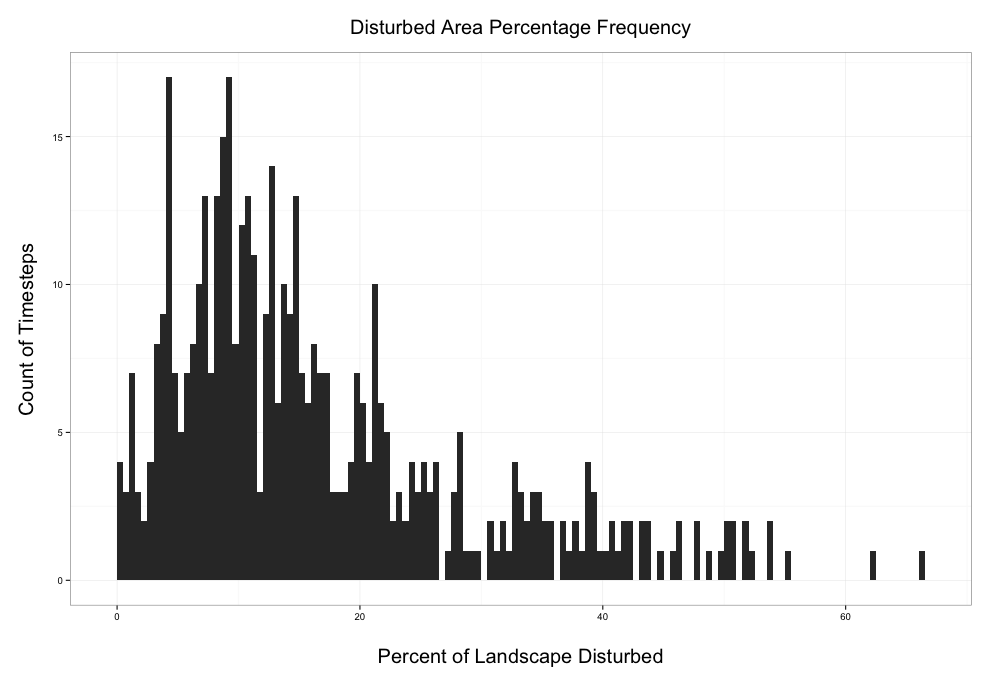
\includegraphics[width=0.6\textwidth]{/Users/mmallek/Tahoe/Report2/images/darea_hist.png}
\caption{Histogram of percent of landscape disturbed by wildfire during the simulation. The distribution is substantially right-skewed, and most fires burn less than 20\% of the eligible landscape.}
\label{fig:darea_hist}
\end{figure}

% background color 24, 15, 41, 0
\todo{figures redone}
\begin{figure}[!htbp]
  \centering
  \subfloat[][]{
    \centering
    \includegraphics[width=0.5\textwidth]{/Users/mmallek/Tahoe/Report2/images/wfmort1250_min.png}
    \label{fig:darea_min}
  }%
  \subfloat[][]{
    \includegraphics[width=0.5\textwidth]{/Users/mmallek/Tahoe/Report2/images/distid1250_min.png}
    \label{fig:distid_min}
  }
  \caption{Maps of area burned during the timestep with the \textbf{least total area burned (0.72\%)} during the simulation. (a) Map by mortality level. Red indicates high mortality fire, while orange indicates low mortality fire. (b) Map showing each individual fire in a different color.}
  \label{fig:darea_min_map}
\end{figure}

\begin{figure}[!htbp]
  \centering
  \subfloat[][]{
    \centering
    \includegraphics[width=0.5\textwidth]{/Users/mmallek/Tahoe/Report2/images/wfmort1340_max.png}
    \label{fig:darea_max}
  }%
  \subfloat[][]{
    \includegraphics[width=0.5\textwidth]{/Users/mmallek/Tahoe/Report2/images/distid1340_max.png}
    \label{fig:distid_max}
  }
  \caption{Maps of area burned during the timestep with the \textbf{most total area burned (72.39\%)} during the simulation. (a) Map by mortality level. Red indicates high mortality fire, while orange indicates low mortality fire. (b) Map showing each individual fire in a different color.}
  \label{fig:darea_max_map}
\end{figure}

\begin{figure}[!htbp]
  \centering
  \subfloat[][]{
    \centering
    \includegraphics[width=0.5\textwidth]{/Users/mmallek/Tahoe/Report2/images/wfmort1945_median.png}
    \label{fig:darea_median}
  }%
  \subfloat[][]{
    \includegraphics[width=0.5\textwidth]{/Users/mmallek/Tahoe/Report2/images/distid1945_median.png}
    \label{fig:distid_median}
  }
  \caption{Maps of area burned during the timestep with the \textbf{median total area burned (14.28\%)} during the simulation. (a) Map by mortality level. Red indicates high mortality fire, while orange indicates low mortality fire. (b) Map showing each individual fire in a different color.}
  \label{fig:darea_median_map}
\end{figure}

\begin{figure}[!htbp]
  \centering
  \subfloat[][]{
    \centering
    \includegraphics[width=0.5\textwidth]{/Users/mmallek/Tahoe/Report2/images/wfmort940_mean.png}
    \label{fig:darea_mean}
  }%
  \subfloat[][]{
    \includegraphics[width=0.5\textwidth]{/Users/mmallek/Tahoe/Report2/images/distid940_mean.png}
    \label{fig:distid_mean}
  }
  \caption{Maps of area burned during the timestep with the \textbf{mean total area burned (17.53\%)} during the simulation. (a) Map by mortality level. Red indicates high mortality fire, while orange indicates low mortality fire. (b) Map showing each individual fire in a different color.}
  \label{fig:darea_mean_map}
\end{figure}

\subsubsection{Disturbance Size}
As described in Section \ref{subsubsec:distparams}, we specified a target set of disturbance sizes. Because wildfire has many stochastic components, we do not expect the model results to match these targets exactly. Figure \ref{fig:dsize} compares the observed and target disturbance size distribution.



\begin{figure}[!htbp]
\centering
\includegraphics[width=0.7\textwidth]{/Users/mmallek/Tahoe/R/Rplots/November2014/dsize.png}
\caption{Side by side barplot of the observed and target wildfire size distribution for our 500-timestep long run of the model.}
\label{fig:dsize}
\end{figure}



\subsubsection{Effect of Climate} Climate does have a positive relationship with disturbed area, as expected (Figure \ref{fig:climate_darea}. We show here a fitted line, but note the heteroskedastic variance about the mean. The relationship is fairly weak. During wetter-than-average years, we see less disturbed area. Over 20\% of the landscape burned only in timesteps during which the climate parameter was at least 0.63. However, over 50\% of the landscape burned in several timesteps when the climate parameter was less than 1, which is the average value over the historical period. Overall we observe that as climate shifts from wet to drought, the disturbed area increases. Climate also has a weak effect on the size of individual fires (Figure \ref{fig:climate_dsize}). Fire size is also influenced by vegetation susceptibility and the specified disturbance size distribution. Figure \ref{fig:compare_clim_darea} illustrates the climate parameter values and disturbed area proportion of the landscape for a subset of timesteps during the simulation.
\todo{the dsize function has something wrong with it (and always did)}
\begin{figure}[!htbp]
  \centering
  \subfloat[][]{
    \centering
    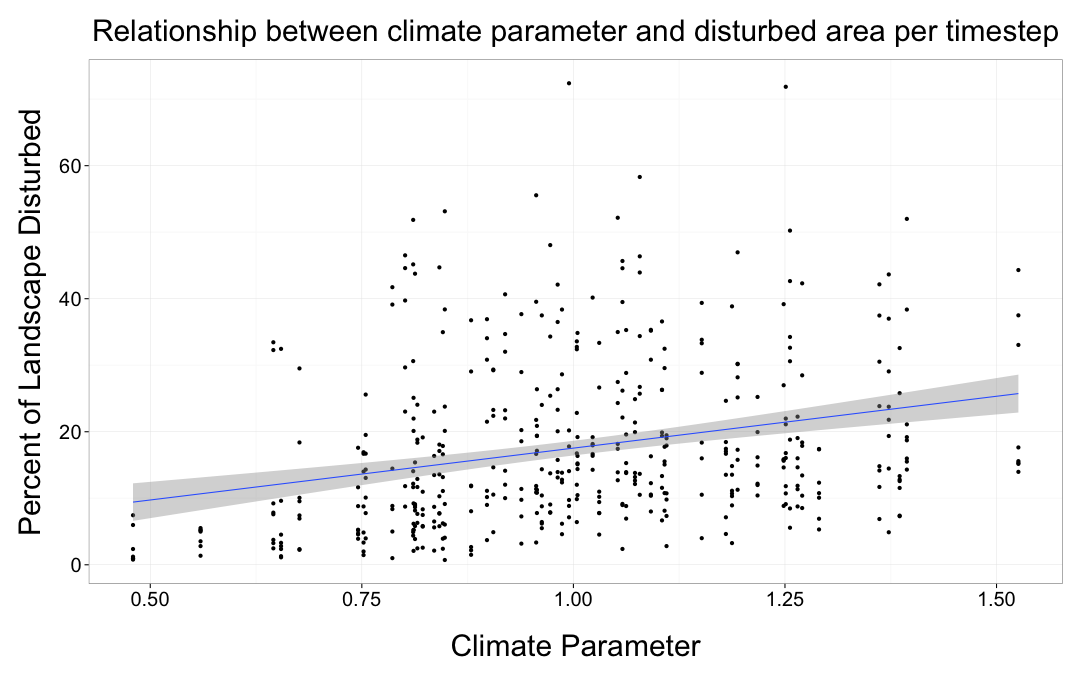
\includegraphics[width=0.5\textwidth]{/Users/mmallek/Tahoe/Report2/images/climate_darea.png}
    \label{fig:climate_darea}
  }%
  %\qquad
 % \subfloat[][]{
 %   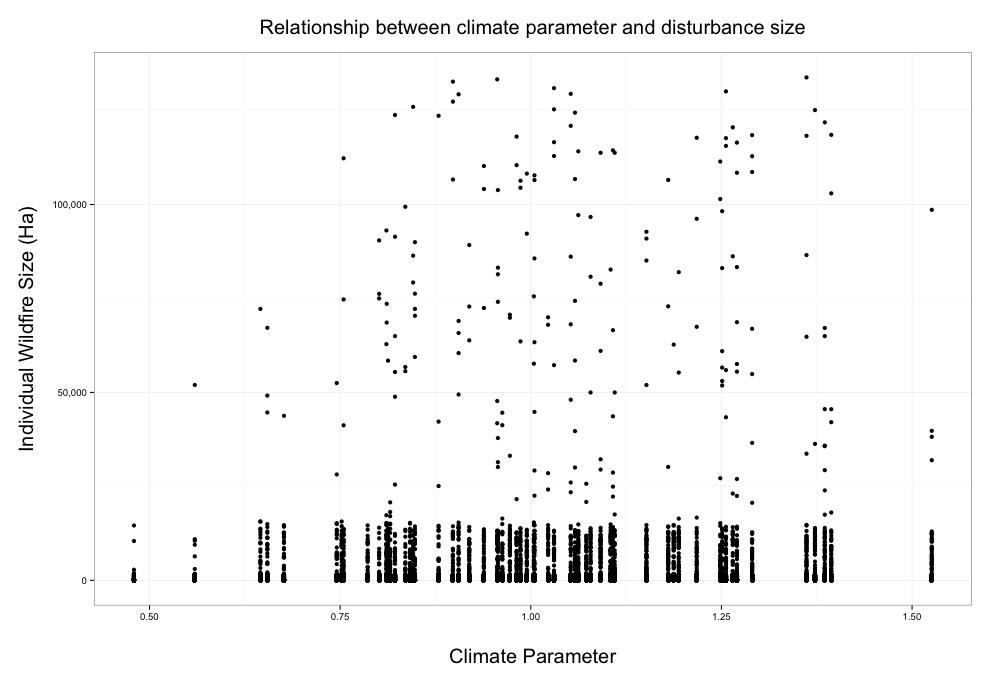
\includegraphics[width=0.5\textwidth]{/Users/mmallek/Tahoe/Report2/images/climate_dsize.png}
 %   \label{fig:climate_dsize}
 % }
  \caption{(a) Plot of the climate parameter and disturbed area value for each timestep of the simulation (excluding the  equilibration period). A linear model has been fit to the data and is shown as a blue line; the grey shaded area represents  the 95\% confidence interval around the mean. (b) Plot showing the size of each individual wildfire and the climate parameter value in effect at the time of disturbance for each disturbance during the simulation (excluding the equilibration period).}
  \label{fig:climate_disturbance}
\end{figure}

\begin{figure}[!htbp]
\centering
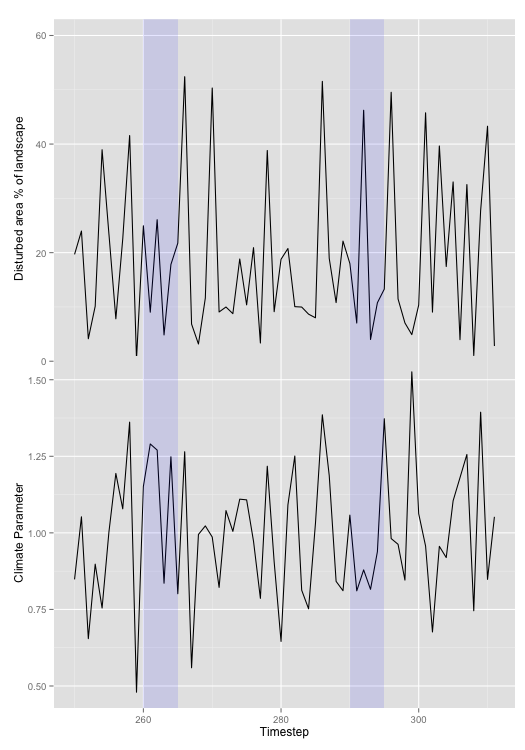
\includegraphics[width=0.8\textwidth]{/Users/mmallek/Tahoe/Report2/images/climate_darea_vert.png}
\caption{Climate parameter and proportion of eligible landscape disturbed by wildfire for timesteps 250 to 310 of the simulation.}
\label{fig:compare_clim_darea}
\end{figure}

\clearpage
\subsubsection{Effect of Topographic Position}\todo{needs to be redone}

The topographic position index value for a given cell acts as an input into the susceptibility and mortality values otherwise defined for that cover type and condition class combination. In general, cells with smaller TPI values had reduced susceptibility and mortality. Early development and open canopy conditions tend to result from fire, and we predicted that an increase in fires and in the likelihood of high mortality fire would lead to a decrease in the average canopy cover values for cells with large TPI values. Table \ref{tab:tpi_cc} displays the results for this simulation for the nine focal cover types. All but one (\textsc{ocfw\_u}) show decreased average canopy cover as TPI increases, with the decrease ranging from 3.3\% in Mixed Evergreen - Mesic to 36.4\% in Sierran Mixed Conifer - Ultramafic. Figure \ref{fig:tpi_cc} shows the plotted data and fitted linear regression line for each of the nine focal types. Figure \ref{fig:averagecc} \todo{Smoothed version on Z Drive} is a map displaying average canopy cover across the landscape for the full simulated HRV timeframe, excluding the equilibration period. \todo{also have a faceted figure that shows all types on the same y axis/scale - for appendix?}

\todo{figure redone}
\begin{figure}[!htbp]
\centering
\includegraphics[width=0.8\textwidth]{/Users/mmallek/Tahoe/Report2/images/averagecc.jpg}
\caption{Smoothed visualization of the average canopy cover across the project area over the course of the simulation. Higher percent cover is shown in blue, transitioning to red where average percent cover was low.}
\label{fig:averagecc}
\end{figure}

\todo{table is updated}
\begin{table}[!htbp]
\caption{For each cover type on the landscape, the percent change in canopy cover from the minimum TPI value for that cover type to the maximum TPI value.}
\label{tab:tpi_cc}
%\rotatebox{90}{
\begin{tabular}{@{}llllll@{}}
\toprule
\small \textbf{\begin{tabular}[c]{@{}l@{}}Cover \\ Name\end{tabular}} & \small \textbf{\begin{tabular}[c]{@{}l@{}}Minimum \\ TPI\end{tabular}} & \small \textbf{\begin{tabular}[c]{@{}l@{}}Maximum \\ TPI\end{tabular}} & \small \textbf{\begin{tabular}[c]{@{}l@{}}Average Canopy \\Cover at \\ Minimum TPI\end{tabular}} & \small \textbf{\begin{tabular}[c]{@{}l@{}}Average Canopy \\ Cover at \\ Maximum TPI\end{tabular}}  & \small \textbf{\begin{tabular}[c]{@{}l@{}}Percent \\ Change in \\ Canopy \\ Cover\end{tabular}} \\ \midrule
MEG\_M       & -300                 & 300                  & 66.5         & 67.5              &  1.5      \\
MEG\_X       & -299                 & 300                  & 64.1         & 66.4              &  3.8      \\
OCFW         & -300                 & 300                  & 49.6         & 46.5              &  -6.2      \\
OCFW\_U      & -300                 & 300                  & 25.0         & 22.8              &  -9.0       \\
RFR\_M       & -300                 & 300                  & 65.2         & 58.9              &  -9.7     \\
RFR\_X       & -259                 & 300                  & 49.0         & 33.0              & -32.4     \\
SMC\_M       & -300                 & 300                  & 48.8         & 42.6              & -12.6      \\
SMC\_U       & -300                 & 300                  & 36.7         & 28.3              & -22.7     \\
SMC\_X       & -300                 & 300                  & 35.9         & 26.9              & -24.9     \\ \bottomrule
\end{tabular}
%}
\end{table}

\todo{figure is redone}
\begin{figure}[!htbp]
\centering
\includegraphics[width=\textwidth]{/Users/mmallek/Tahoe/Report2/images/TPI_cc_focaltypes.png}
\label{fig:tpi_cc_focaltypes}
\caption{Average canopy cover for the nine focal cover types during the simulated. Each blue point represents one pixel of an individual cover type on the landscape grid. The black line is the result of a linear regression fit to the data. Table \ref{tab:tpi_cc} provides the numerical representation of the shift from minimum to maximum TPI values for each cover type. (a) Mixed Evergreen - Mesic; (b) Mixed Evergreen - Xeric; (c) Oak-Conifer Forest and Woodland; (d) Oak-Conifer Forest and Woodland - Ultramafic; (e) Red Fir - Mesic; (f) Red Fir - Xeric; (g) Sierran Mixed Conifer - Mesic; (h) Sierran Mixed Conifer - Ultramafic; (i) Sierran Mixed Conifer - Xeric.}
\label{fig:tpi_cc}
\end{figure}


%\begin{figure}[!htbp]
%  \centering
%  \subfloat[][]{
%    \centering
%    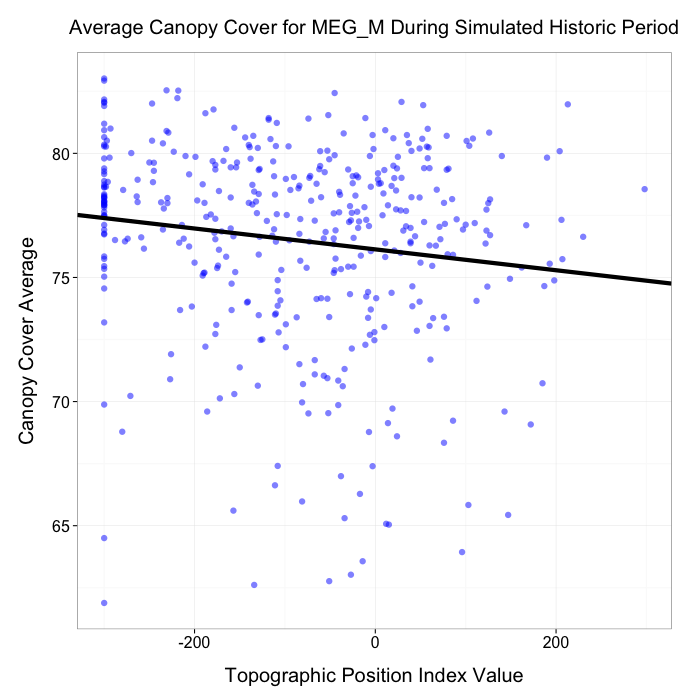
\includegraphics[width=0.33\textwidth]{/Users/mmallek/Tahoe/Report2/images/TPI_cc_megm.png}
%    \label{fig:tpi_cc_megm}
%  }%
%  \subfloat[][]{
%    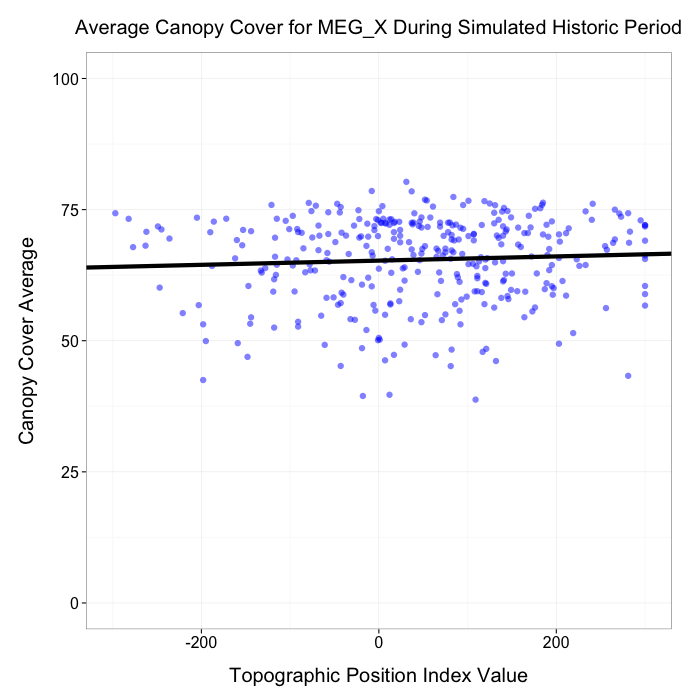
\includegraphics[width=0.33\textwidth]{/Users/mmallek/Tahoe/Report2/images/TPI_cc_megx.png}
%    \label{fig:tpi_cc_megx}
%  }%
%  \subfloat[][]{
%    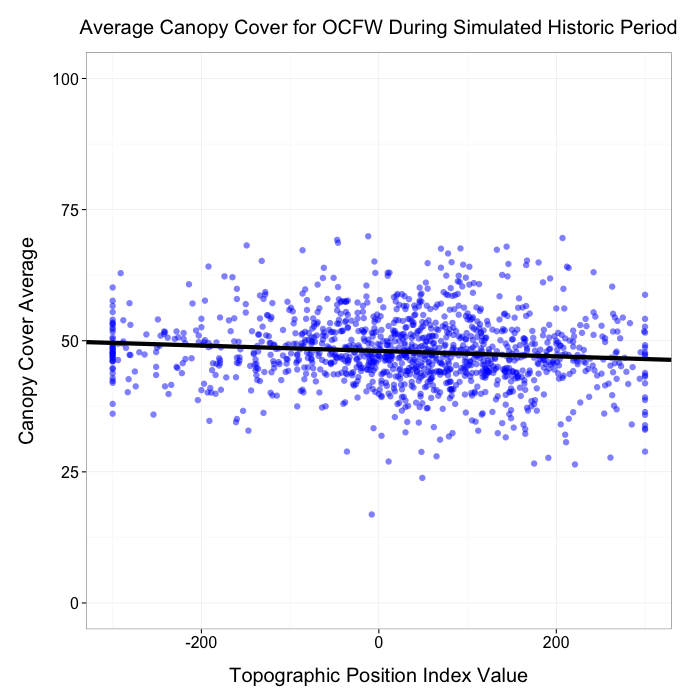
\includegraphics[width=0.33\textwidth]{/Users/mmallek/Tahoe/Report2/images/TPI_cc_ocfw.png}
%    \label{fig:ocfw}
%    }
%
%  \subfloat[][]{
%    \centering
%    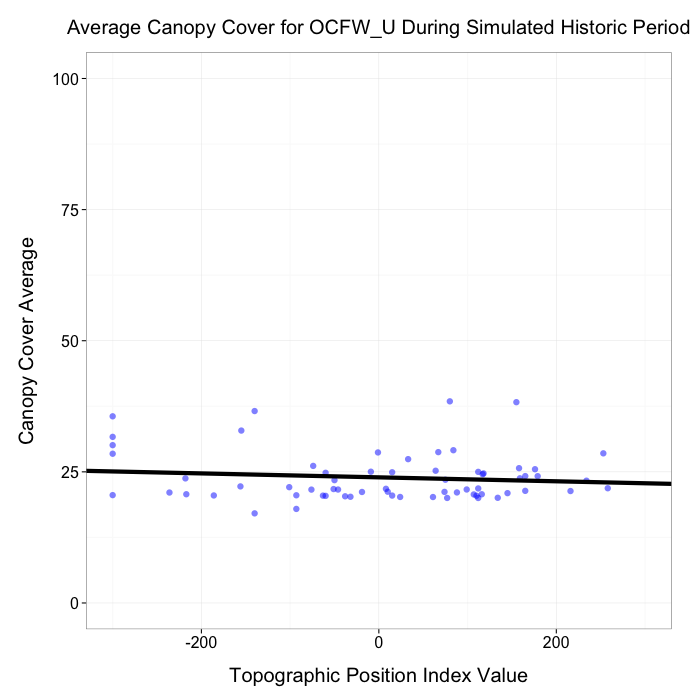
\includegraphics[width=0.33\textwidth]{/Users/mmallek/Tahoe/Report2/images/TPI_cc_ocfwu.png}
%    \label{fig:tpi_cc_ocfwu}
%  }%
%  \subfloat[][]{
%    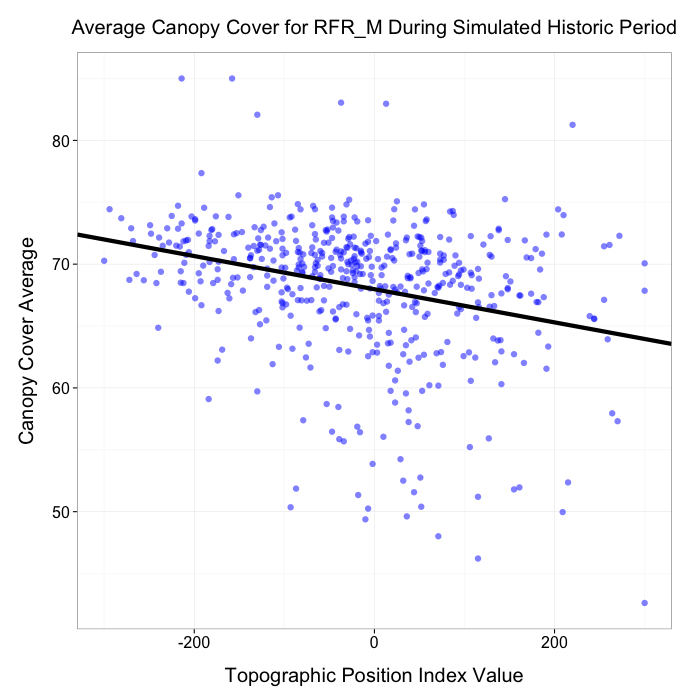
\includegraphics[width=0.33\textwidth]{/Users/mmallek/Tahoe/Report2/images/TPI_cc_rfrm.png}
%    \label{fig:tpi_cc_rfrm}
%  }%
%  \subfloat[][]{
%    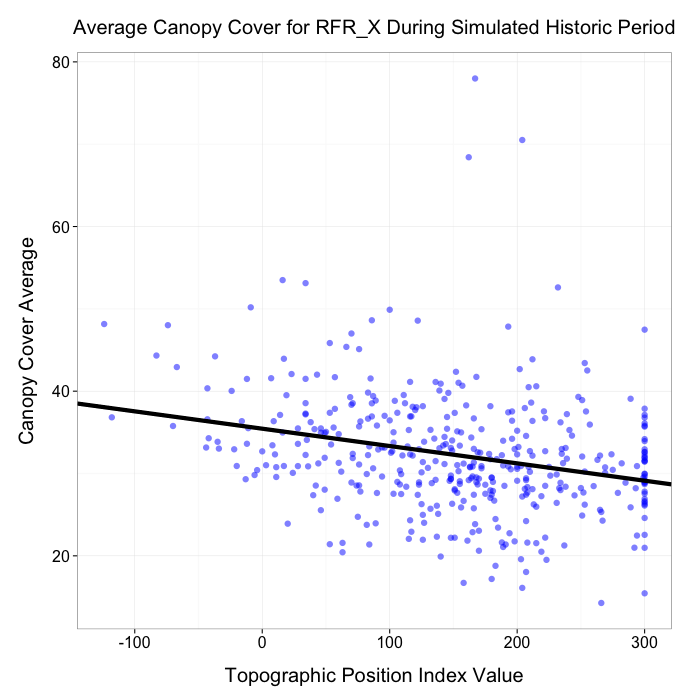
\includegraphics[width=0.33\textwidth]{/Users/mmallek/Tahoe/Report2/images/TPI_cc_rfrx.png}
%    \label{fig:tpi_cc_rfrx}
%    }
%
%  \subfloat[][]{
%    \centering
%    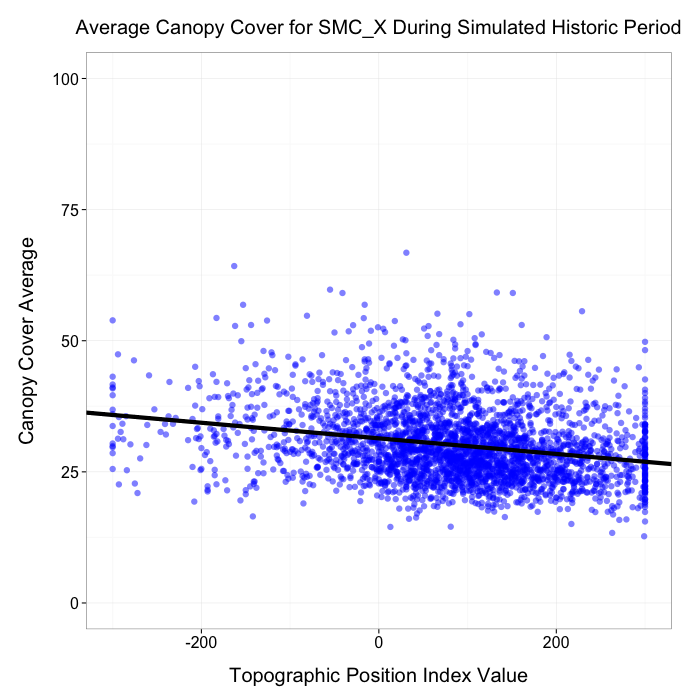
\includegraphics[width=0.33\textwidth]{/Users/mmallek/Tahoe/Report2/images/TPI_cc_smcx.png}
%    \label{fig:tpi_cc_smcm}
%  }%
%  \subfloat[][]{
%    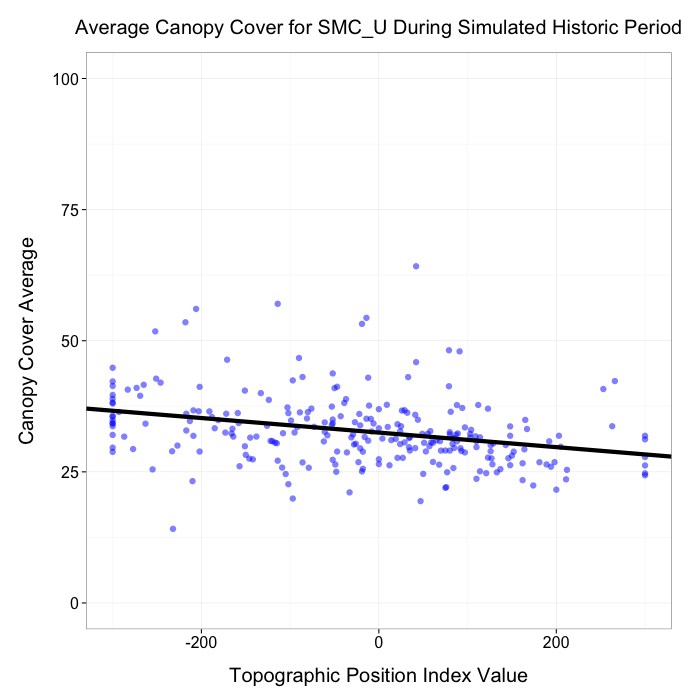
\includegraphics[width=0.33\textwidth]{/Users/mmallek/Tahoe/Report2/images/TPI_cc_smcu.png}
%    \label{fig:tpi_cc_smcu}
%  }%
%  \subfloat[][]{
%    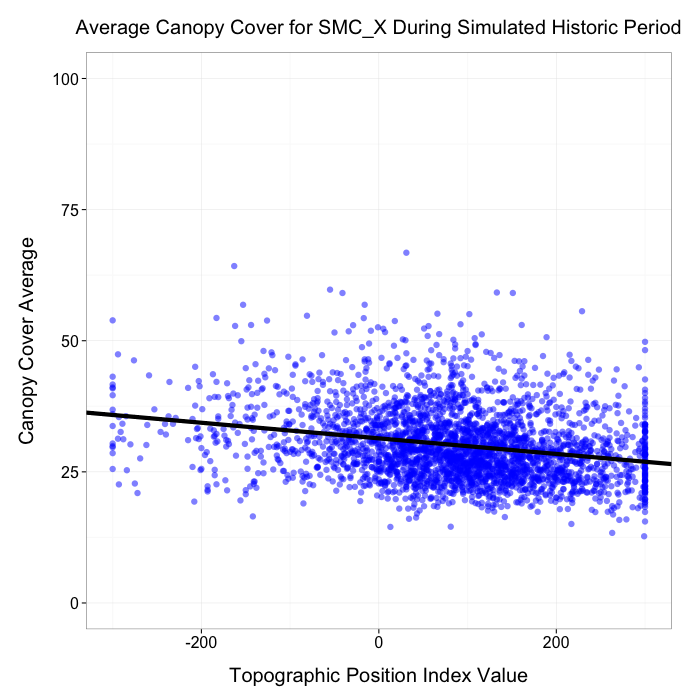
\includegraphics[width=0.33\textwidth]{/Users/mmallek/Tahoe/Report2/images/TPI_cc_smcx.png}
%    \label{fig:tpi_cc_smcx}
%    }
%  \caption{Average canopy cover for the nine focal cover types during the simulated. Each blue point represents one pixel of an individual cover type on the landscape grid. The black line is the result of a linear regression fit to the data. Note, the $y$ axis is scaled differently across cover types in order to more easily focus on the data for each type. Table \ref{tab:tpi_cc} provides the numerical representation of the shift from minimum to maximum TPI values for each cover type. (a) Mixed Evergreen - Mesic; (b) Mixed Evergreen - Xeric; (c) Oak-Conifer Forest and Woodland; (d) Oak-Conifer Forest and Woodland - Ultramafic; (e) Red Fir - Mesic; (f) Red Fir - Xeric; (g) Sierran Mixed Conifer - Mesic; (h) Sierran Mixed Conifer - Ultramafic; (i) Sierran Mixed Conifer - Xeric.}
%  \label{fig:tpi_cc}
%\end{figure}



\newpage
\subsubsection{Fire Rotation}
We present here the results for non-static cover types whose extent is at least 1000 ha. Full results are presented in Appendix \ref{sec:full-rot-results}. As previously discussed, these results could have been presented in the methods section. Each of the nine cover types shown here were calibrated to within 10\% of their target values, which were based on empirical published values and local expert opinion.
\todo{this has been updated}
\begin{table}[!htbp]
\centering
\caption{Fire rotation for the nine cover types whose extent cover at least 1000 ha.}
\begin{tabular}{@{}llll@{}}
\toprule
Land Cover Type                              & \begin{tabular}[c]{@{}l@{}}Low Mortality \\ Fire Rotation\end{tabular} & \begin{tabular}[c]{@{}l@{}}High Mortality \\ Fire Rotation\end{tabular} & \begin{tabular}[c]{@{}l@{}}All Fires \\ Rotation\end{tabular} \\ \midrule
Mixed Evergreen - Mesic                      & 61                          & 525                          & 55                 \\
Mixed Evergreen - Xeric                      & 47                          & 434                          & 42                 \\
Oak-Conifer Forest and Woodland              & 30                          & 115                          & 24                 \\
\begin{tabular}[c]{@{}l@{}}Oak-Conifer Forest and \\ \hspace{5em}Woodland -  Ultramafic\end{tabular} & 44                          & 1295                         & 43                 \\
Red Fir - Mesic                              & 102                         & 160                          & 62                 \\
Red Fir - Xeric                              & 62                          & 108                          & 39                 \\
Sierran Mixed Conifer - Mesic                & 36                          & 125                          & 28                 \\
Sierran Mixed Conifer - Ultramafic           & 94                          & 196                          & 63                 \\
Sierran Mixed Conifer - Xeric                & 36                          & 64                           & 23                 \\
Total                                        & 41                          & 106                          & 30                 \\ \bottomrule
\end{tabular}
\end{table}


\subsubsection{Population Return Interval}
Overall, the point-specific return interval (grand mean) for all eligible cells ranged from 17 years to \textgreater 2500 years (cells that never burned during the simulation) for both classes of wildfire mortality (Figure \ref{fig:preturn}. The median return interval across all cover types was 42 years for low mortality fire, 111 year for high mortality fire, and 29 years for any fire. The population return interval plots and maps specific to each of the nine focal cover types follow (Figures \ref{fig:preturn_megm} through \ref{fig:preturn_smcx}.). We compare the current landscape's seral stage distribution to the simulated distribution and compute the HRV departure index in Tables \ref{tab:covcond1} and \ref{tab:covcond2}.
\todo{updated preturn R plots but not arcmap plots - maybe can skip until post-presentation?}
\begin{figure}[!htbp]
  \centering
  \subfloat[][]{
    \centering
    \includegraphics[height=0.4\textheight]{/Users/mmallek/Tahoe/R/Rplots/November2014/preturn_all.png}
    \label{fig:preturn_plot}
  }%
  \qquad
  \subfloat[][]{
    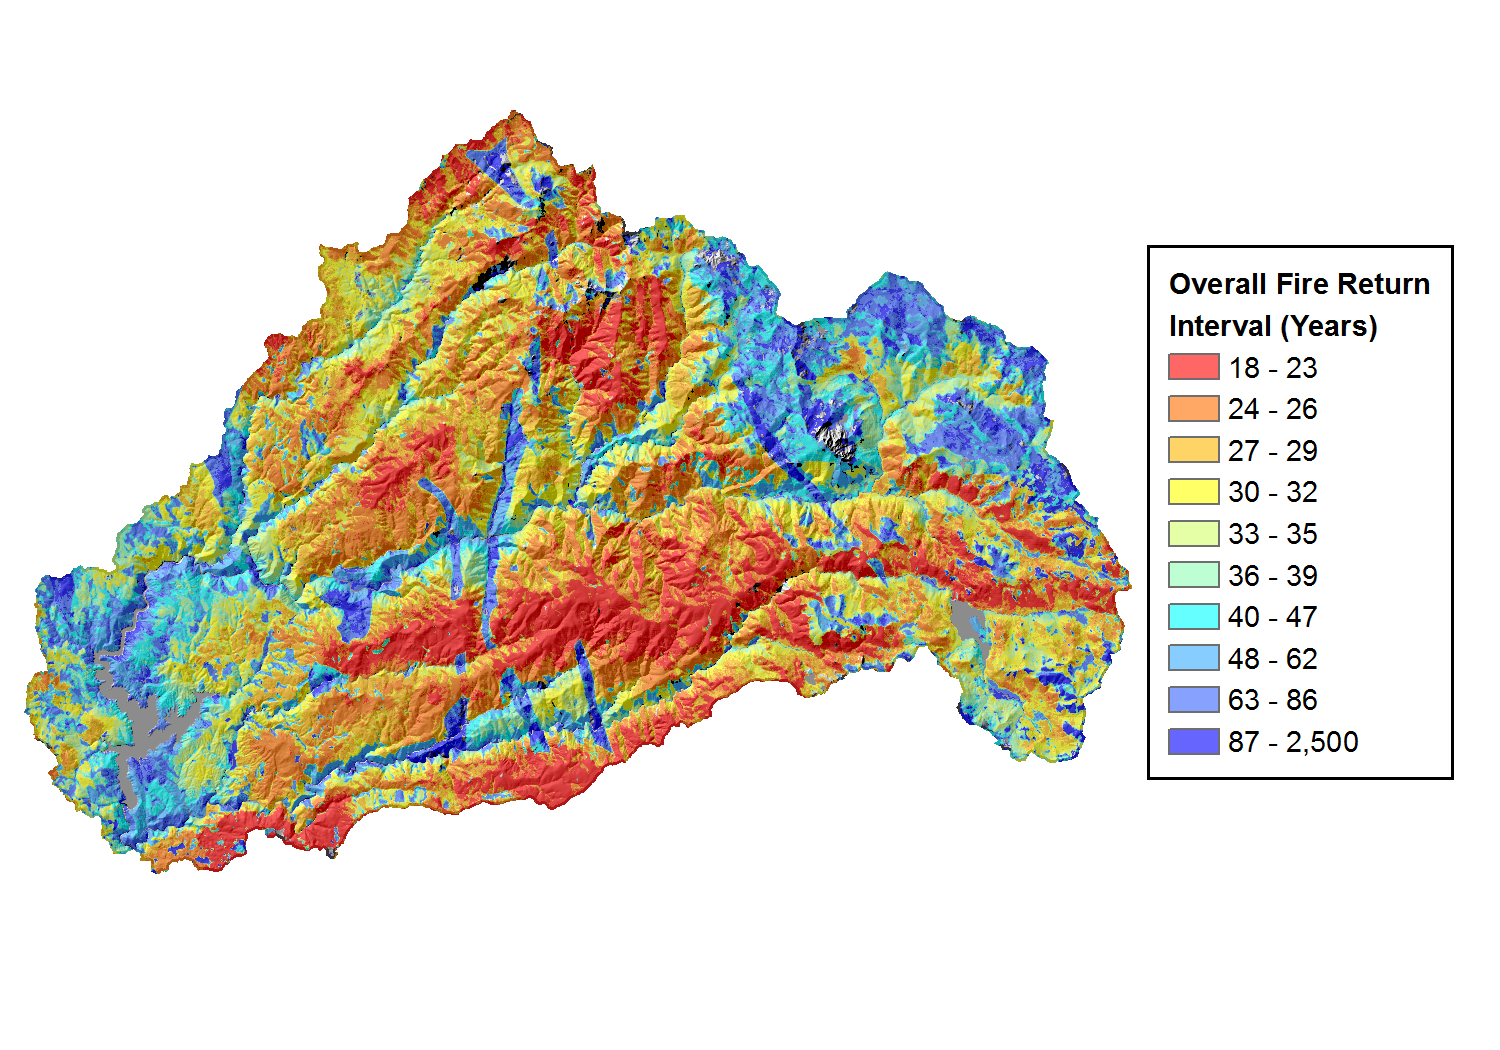
\includegraphics[height=0.4\textheight]{/Users/mmallek/Tahoe/Report2/images/fri_all.png}
    \label{fig:preturn_map}
  }
  \caption{(a) Population return interval (average number of years between fires) distribution for the full landscape under study. The population return interval is the point-specific interval, sometimes described as the ``grand mean'' for a given point. (b) Spatial depiction of fire return intervals across the landscape, for all cover types, in terms of fire return interval. The value at any given cell is the point-specific return interval.}
  \label{fig:preturn}
\end{figure}


\begin{figure}[!htbp]
  \centering
  \subfloat[][]{
    \centering
    \includegraphics[width=0.5\textwidth]{/Users/mmallek/Tahoe/R/Rplots/November2014/preturn_megm.png}
    }%
  \subfloat[][]{
    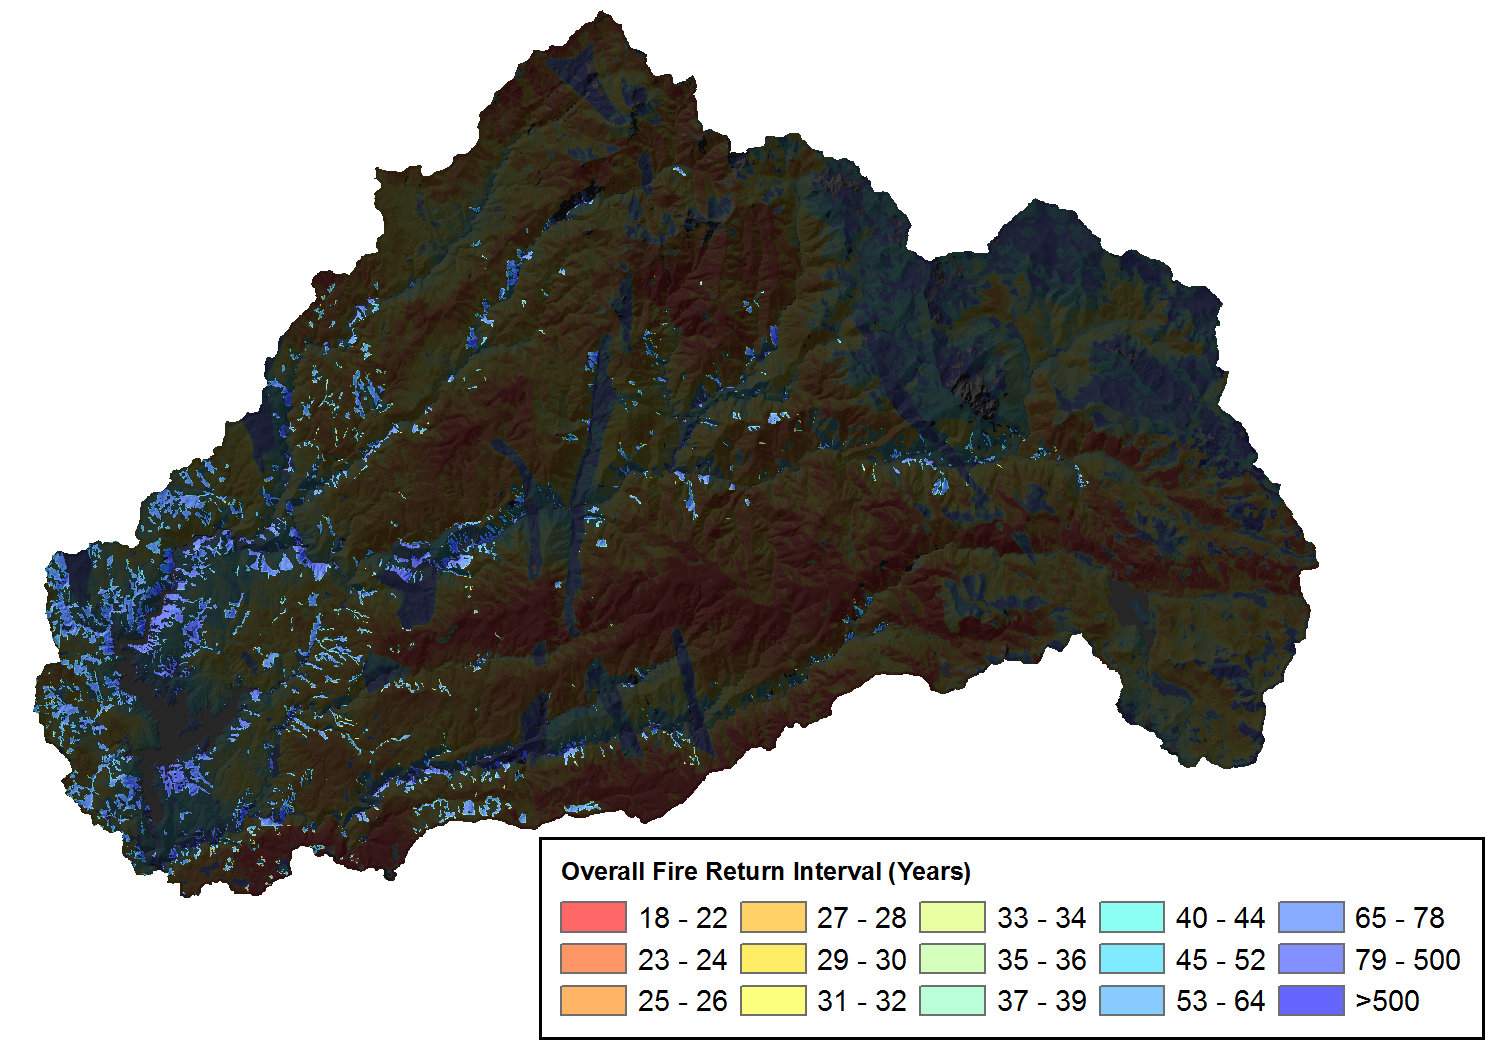
\includegraphics[width=0.5\textwidth]{/Users/mmallek/Tahoe/Report2/images/fri_megm.png}
    }
  \caption{(a) Population return interval (average number of years between fires) distribution for Mixed Evergreen - Mesic. (b) Spatial depiction of fire return intervals across the landscape. Cover types other than Mixed Evergreen - Mesic are partially obscured in grey. The value at any given cell is the point-specific return interval, which ranges from 20 years to \textgreater 500 years.}
    \label{fig:preturn_megm}
\end{figure}

\begin{figure}[!htbp]
  \centering
  \subfloat[][]{
    \centering
    \includegraphics[width=0.5\textwidth]{/Users/mmallek/Tahoe/R/Rplots/November2014/preturn_megx.png}
    }%
  \subfloat[][]{
    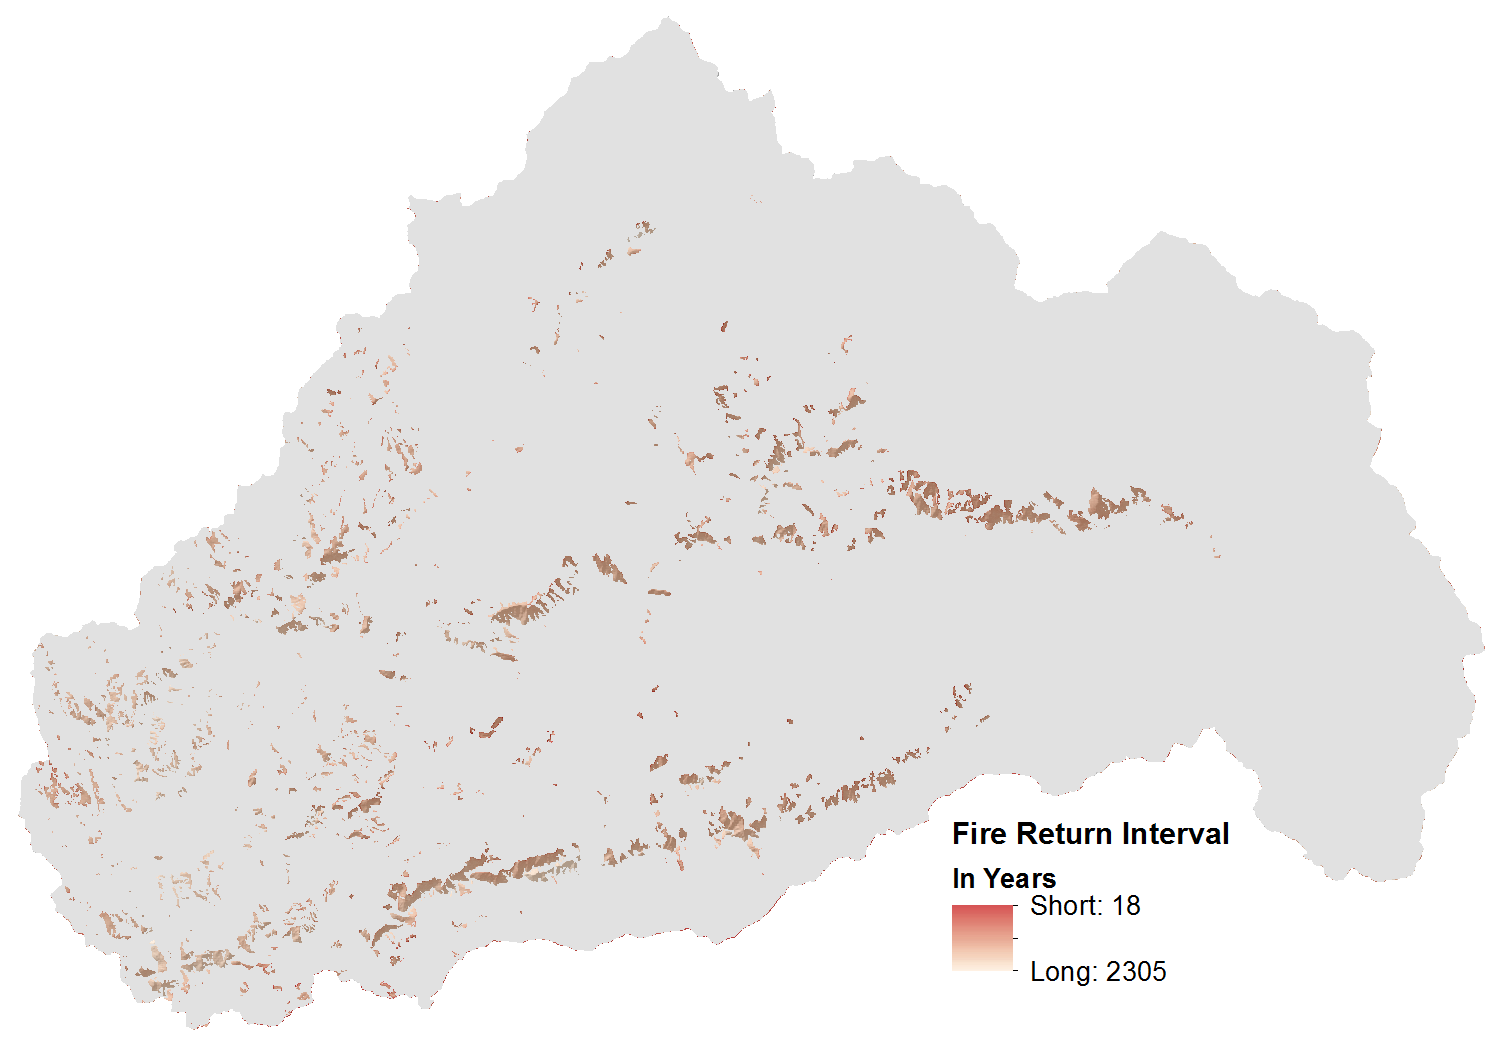
\includegraphics[width=0.5\textwidth]{/Users/mmallek/Tahoe/Report2/images/fri_megx.png}
    }
  \caption{(a) Population return interval (average number of years between fires) distribution for Mixed Evergreen - Xeric.  (b) Spatial depiction of fire return intervals across the landscape. Cover types other than Mixed Evergreen - Xeric are partially obscured in grey. The value at any given cell is the point-specific return interval, which ranges from 19 years to \textgreater 500 years.}
\label{fig:preturn_megx}
\end{figure}

\begin{figure}[!htbp]
  \centering
  \subfloat[][]{
    \centering
    \includegraphics[width=0.5\textwidth]{/Users/mmallek/Tahoe/R/Rplots/November2014/preturn_ocfw.png}
    }%
  \subfloat[][]{
    \includegraphics[width=0.5\textwidth]{/Users/mmallek/Tahoe/Report2/images/fri_ocfw.png}
    }
  \caption{(a) Population return interval (average number of years between fires) distribution for Oak-Conifer Forest and Woodland.  (b) Spatial depiction of fire return intervals across the landscape. Cover types other than Oak-Conifer Forest and Woodland are partially obscured in grey. The value at any given cell is the point-specific return interval, which ranges from 17 years to \textgreater 500 years.}
\label{fig:preturn_ocfw}
\end{figure}

\begin{figure}[!htbp]
  \centering
  \subfloat[][]{
    \centering
    \includegraphics[width=0.5\textwidth]{/Users/mmallek/Tahoe/R/Rplots/November2014/preturn_ocfwu.png}
    }%
  \subfloat[][]{
    \includegraphics[width=0.5\textwidth]{/Users/mmallek/Tahoe/Report2/images/fri_ocfwu.png}
    }
  \caption{(a) Population return interval (average number of years between fires) distribution for Oak-Conifer Forest and Woodland - Ultramafic.  (b) Spatial depiction of fire return intervals across the landscape. Cover types other than Oak-Conifer Forest and Woodland - Ultramafic are partially obscured in grey. The value at any given cell is the point-specific return interval, which ranges from 20 years to \textgreater 500 years.}
\label{fig:preturn_ocfwu}
\end{figure}

\begin{figure}[!htbp]
  \centering
  \subfloat[][]{
    \centering
    \includegraphics[width=0.5\textwidth]{/Users/mmallek/Tahoe/R/Rplots/November2014/preturn_rfrm.png}
    }%
  \subfloat[][]{
    \includegraphics[width=0.5\textwidth]{/Users/mmallek/Tahoe/Report2/images/fri_rfrm.png}
    }
  \caption{(a) Population return interval (average number of years between fires) distribution for Red Fir - Mesic.  (b) Spatial depiction of fire return intervals across the landscape. Cover types other than Red Fir - Mesic are partially obscured in grey. The value at any given cell is the point-specific return interval, which ranges from 20 years to \textgreater 500 years.}
\label{fig:preturn_rfrm}
\end{figure}

\begin{figure}[!htbp]
  \centering
  \subfloat[][]{
    \centering
    \includegraphics[width=0.5\textwidth]{/Users/mmallek/Tahoe/R/Rplots/November2014/preturn_rfrx.png}
    }%
  \subfloat[][]{
    \includegraphics[width=0.5\textwidth]{/Users/mmallek/Tahoe/Report2/images/fri_rfrx.png}
    }
  \caption{(a) Population return interval (average number of years between fires) distribution for Red Fir - Xeric.  (b) Spatial depiction of fire return intervals across the landscape. Cover types other than Red Fir - Xeric are partially obscured in grey. The value at any given cell is the point-specific return interval, which ranges from 19 years to \textgreater 500 years.}
\label{fig:preturn_rfrx}
\end{figure}

\begin{figure}[!htbp]
  \centering
  \subfloat[][]{
    \centering
    \includegraphics[width=0.5\textwidth]{/Users/mmallek/Tahoe/R/Rplots/November2014/preturn_smcm.png}
    }%
  \subfloat[][]{
    \includegraphics[width=0.5\textwidth]{/Users/mmallek/Tahoe/Report2/images/fri_smcm.png}
    }
  \caption{(a) Population return interval (average number of years between fires) distribution for Sierran Mixed Conifer - Mesic.  (b) Spatial depiction of fire return intervals across the landscape. Cover types other than Sierran Mixed Conifer - Mesic are partially obscured in grey. The value at any given cell is the point-specific return interval, which ranges from 18 years to \textgreater 500 years.}
\label{fig:preturn_smcm}
\end{figure}

\begin{figure}[!htbp]
  \centering
  \subfloat[][]{
    \centering
    \includegraphics[width=0.5\textwidth]{/Users/mmallek/Tahoe/R/Rplots/November2014/preturn_smcu.png}
    }%
  \subfloat[][]{
    \includegraphics[width=0.5\textwidth]{/Users/mmallek/Tahoe/Report2/images/fri_smcu.png}
    }
  \caption{(a) Population return interval (average number of years between fires) distribution for Sierran Mixed Conifer - Ultramafic.  (b) Spatial depiction of fire return intervals across the landscape. Cover types other than Sierran Mixed Conifer - Ultramafic are partially obscured in grey. The value at any given cell is the point-specific return interval, which ranges from 21 years to \textgreater 500 years.}
\label{fig:preturn_smcu}
\end{figure}

\begin{figure}[!htbp]
  \centering
  \subfloat[][]{
    \centering
    \includegraphics[width=0.5\textwidth]{/Users/mmallek/Tahoe/R/Rplots/November2014/preturn_smcx.png}
    }%
  \subfloat[][]{
    \includegraphics[width=0.5\textwidth]{/Users/mmallek/Tahoe/Report2/images/fri_smcx.png}
    }
  \caption{(a) Population return interval (average number of years between fires) distribution for Sierran Mixed Conifer - Xeric.  (b) Spatial depiction of fire return intervals across the landscape. Cover types other than Sierran Mixed Conifer - Xeric are partially obscured in grey. The value at any given cell is the point-specific return interval, which ranges from 17 years to \textgreater 500 years.}
\label{fig:preturn_smcx}
\end{figure}

\clearpage

%%%%%%%%%%%%%%%%%%%%%%%%%%%%%%%%
%%%%%%%%%%%%%%%%%%%%%%%%%%%%%%%%
%%%%%%%%%%%%%%%%%%%%%%%%%%%%%%%%
%\pagebreak[4]
\subsection{Vegetation Response}
\label{subsec:HRVvegresponse}

\subsubsection{Condition Sequence}

Condition classes for each cover type varied over time. Evidence of both high mortality fire, which triggers a transition to early development conditions for all cover type, and low mortality fire, which can thin a stand and cause a transition to a more open canopy condition (within the same developmental stage), are visible in examining the output grids. Figure \ref{fig:covcondmaps} illustrates these changes for a sequence of four timesteps during the simulation.
\todo{these have been fixed}
\begin{figure}[!htbp]
  \centering
  \subfloat[][]{
    \includegraphics[width=0.5\textwidth]{/Users/mmallek/Tahoe/Report2/images/covcond660.png}
  }%
  \subfloat[][]{
    \includegraphics[width=0.5\textwidth]{/Users/mmallek/Tahoe/Report2/images/covcond665.png}
  }\\%
  \subfloat[][]{
    \includegraphics[width=0.5\textwidth]{/Users/mmallek/Tahoe/Report2/images/covcond670.png}
    }
  \subfloat[][]{
    \centering
    \includegraphics[width=0.5\textwidth]{/Users/mmallek/Tahoe/Report2/images/covcond675.png}
  }%
  \caption{A sequence of four timesteps during the simulation, showing changes in condition classes over time. Here we highlight the dominant cover type, Sierran Mixed Conifer - Mesic, and its classes, in order to illustrate the dynamics that play out over many years. (a) Timestep 660 (b) Timestep 665 (c) Timestep 670 (d) Timestep 675.}
  \label{fig:covcondmaps}
\end{figure}

\subsubsection{Landscape Composition}

The distribution of area among condition classes within all cover types fluctuated over time, as expected. The relative proportion of each condition class also varied across cover types. In general, the condition class distribution appeared to be in dynamic equilibrium, despite considerable variability from timestep to timestep. The exception is the Oak-Conifer Forest and Woodland cover type, which did not appear to reach equilibrium until around timestep 220. The cover-condition dynamics and current seral stage distribution plots specific to each of the nine focal cover types follow (Figures \ref{fig:covcond_megm} through \ref{fig:covcond_smcx}.).

A few patterns emerge across the nine focal cover types. A numerical representation of these dynamics is available in Tables \ref{tab:covcond1} to \ref{tab:covcond3}. In general, early seral conditions were more common during the simulated historic period than on the current landscape. In mesic red fir and sierran mixed conifer forests, closed canopy conditions occupied a greater proportion of the total landscape during the simulated historic period than on the current landscape. In xeric mixed conifer forests, closed canopies were uncommon throughout the simulated period, but occupy 36.68\% of the current landscape.
\todo{all these plots are redone}
\begin{figure}[!htbp]
  \centering
  \subfloat[][]{
    \centering
    \includegraphics[width=0.6\textwidth]{/Users/mmallek/Tahoe/R/Rplots/November2014/covcond_megm.png}
    }%
  \subfloat[][]{
  \centering
  \includegraphics[height=2.65in]{/Users/mmallek/Tahoe/R/Rplots/November2014/covcond_current_megm.png}
    }
  \caption{(a) Cover-Condition dynamics for Mixed Evergreen - Mesic. The black vertical line at 40 timesteps marks the end of the equilibration period used in this study. (b) Current seral stage distribution for Mixed Evergreen - Mesic.}
\label{fig:covcond_megm}
\end{figure}

%\clearpage

\begin{figure}[!htbp]
  \centering
  \subfloat[][]{
    \centering
    \includegraphics[width=0.6\textwidth]{/Users/mmallek/Tahoe/R/Rplots/November2014/covcond_megx.png}
    }%
  \subfloat[][]{
    \includegraphics[height=2.65in]{/Users/mmallek/Tahoe/R/Rplots/November2014/covcond_current_megx.png}
    }
  \caption{(a) Cover-Condition dynamics for Mixed Evergreen - Xeric. The black vertical line at 40 timesteps marks the end of the equilibration period used in this study. (b) Current seral stage distribution for Mixed Evergreen - Xeric.} 
  \label{fig:covcond_megx}
\end{figure}

\begin{figure}[!htbp]
  \centering
  \subfloat[][]{
    \centering
    \includegraphics[width=0.6\textwidth]{/Users/mmallek/Tahoe/R/Rplots/November2014/covcond_ocfw.png}
    }%
  \subfloat[][]{
    \includegraphics[height=2.65in]{/Users/mmallek/Tahoe/R/Rplots/November2014/covcond_current_ocfw.png}
    }
  \caption{(a) Cover-Condition dynamics for Oak-Conifer Forest and Woodland. The black vertical line at 40 timesteps marks the end of the equilibration period used in this study. (b) Current seral stage distribution for Oak-Conifer Forest and Woodland.} 
  \label{fig:covcond_ocfw}
\end{figure}

\begin{figure}[!htbp]
  \centering
  \subfloat[][]{
    \centering
    \includegraphics[width=0.6\textwidth]{/Users/mmallek/Tahoe/R/Rplots/November2014/covcond_ocfwu.png}
    }%
  \subfloat[][]{
    \includegraphics[height=2.65in]{/Users/mmallek/Tahoe/R/Rplots/November2014/covcond_current_ocfwu.png}
    }
  \caption{(a) Cover-Condition dynamics for Oak-Conifer Forest and Woodland - Ultramafic. The black vertical line at 40 timesteps marks the end of the equilibration period used in this study. (b) Current seral stage distribution for Oak-Conifer Forest and Woodland - Ultramafic.} 
  \label{fig:covcond_ocfwu}
\end{figure}

\begin{figure}[!htbp]
  \centering
  \subfloat[][]{
    \centering
    \includegraphics[width=0.6\textwidth]{/Users/mmallek/Tahoe/R/Rplots/November2014/covcond_rfrm.png}
    }%
  \subfloat[][]{
    \includegraphics[height=2.65in]{/Users/mmallek/Tahoe/R/Rplots/November2014/covcond_current_rfrm.png}
    }
  \caption{(a) Cover-Condition dynamics for Red Fir - Mesic. The black vertical line at 40 timesteps marks the end of the equilibration period used in this study. (b) Current seral stage distribution for Red Fir - Mesic.} 
  \label{fig:covcond_rfrm}
\end{figure}

\begin{figure}[!htbp]
  \centering
  \subfloat[][]{
    \centering
    \includegraphics[width=0.6\textwidth]{/Users/mmallek/Tahoe/R/Rplots/November2014/covcond_rfrx.png}
    }%
  \subfloat[][]{
    \includegraphics[height=2.65in]{/Users/mmallek/Tahoe/R/Rplots/November2014/covcond_current_rfrx.png}
    }
  \caption{(a) Cover-Condition dynamics for Red Fir - Xeric. The black vertical line at 40 timesteps marks the end of the equilibration period used in this study. (b) Current seral stage distribution for Red Fir - Xeric.} 
  \label{fig:covcond_rfrx}
\end{figure}

\begin{figure}[!htbp]
  \centering
  \subfloat[][]{
    \centering
    \includegraphics[width=0.6\textwidth]{/Users/mmallek/Tahoe/R/Rplots/November2014/covcond_smcm.png}
    }%
  \subfloat[][]{
    \includegraphics[height=2.65in]{/Users/mmallek/Tahoe/R/Rplots/November2014/covcond_current_smcm.png}
    }
  \caption{(a) Cover-Condition dynamics for Sierran Mixed Conifer - Mesic. The black vertical line at 40 timesteps marks the end of the equilibration period used in this study. (b) Current seral stage distribution for Sierran Mixed Conifer - Mesic.} 
  \label{fig:covcond_smcm}
\end{figure}

\begin{figure}[!htbp]
  \centering
  \subfloat[][]{
    \centering
    \includegraphics[width=0.6\textwidth]{/Users/mmallek/Tahoe/R/Rplots/November2014/covcond_smcu.png}
    }%
  \subfloat[][]{
    \includegraphics[height=2.65in]{/Users/mmallek/Tahoe/R/Rplots/November2014/covcond_current_smcu.png}
    }
  \caption{(a) Cover-Condition dynamics for Sierran Mixed Conifer - Ultramafic. The black vertical line at 40 timesteps marks the end of the equilibration period used in this study. (b) Current seral stage distribution for Sierran Mixed Conifer - Ultramafic.} 
  \label{fig:covcond_smcu}
\end{figure}

\begin{figure}[!htbp]
  \centering
  \subfloat[][]{
    \centering
    \includegraphics[width=0.6\textwidth]{/Users/mmallek/Tahoe/R/Rplots/November2014/covcond_smcx.png}
    }%
  \subfloat[][]{
    \includegraphics[height=2.65in]{/Users/mmallek/Tahoe/R/Rplots/November2014/covcond_current_smcx.png}
    }
  \caption{(a) Cover-Condition dynamics for Sierran Mixed Conifer - Xeric. The black vertical line at 40 timesteps marks the end of the equilibration period used in this study. (b) Current seral stage distribution for Sierran Mixed Conifer - Xeric.} 
  \label{fig:covcond_smcx}
\end{figure}



\todo{the covcond table has been redone}
\begin{landscape}
\begin{table}[!htbp]
\caption{Range of variation in landscape structure, illustrating the cover-condition class dynamics for Mixed Evergreen - Mesic (\textsc{meg\_m}), Mixed Evergreen - Xeric (\textsc{meg\_x}), Oak-Conifer Forest and Woodland (\textsc{ocfw}), and Oak-Conifer Forest and Woodland - Ultramafic (\textsc{ocfw\_u}). For condition class abbreviations, see Table \ref{condtable}.}
\label{tab:covcond1}
\begin{tabular}{@{}lllllllllllll@{}}
\toprule
\footnotesize \textbf{\begin{tabular}[c]{@{}l@{}}Land \\ Cover\\ Type\end{tabular}} & \footnotesize \textbf{\begin{tabular}[c]{@{}l@{}}Condition \\ Class\end{tabular}} & \footnotesize \textbf{srv0\%} & \footnotesize \textbf{srv5\%} & \footnotesize \textbf{srv25\%} & \footnotesize \textbf{srv50\%} & \footnotesize \textbf{srv75\%} & \footnotesize \textbf{srv95\%} & \footnotesize \textbf{srv100\%}   & \footnotesize \textbf{\begin{tabular}[c]{@{}l@{}}Current\\ \%cover\end{tabular}} & \textbf{\begin{tabular}[c]{@{}l@{}}Current\\ \%srv\end{tabular}} & \textbf{\begin{tabular}[c]{@{}l@{}}Departure\\ Index\end{tabular}} \\ \midrule
\footnotesize \textsc{meg\_m}      & \footnotesize \textsc{early\_all}                & \footnotesize 0.22          & \footnotesize 1.19           & \footnotesize 2.13             & \footnotesize 3.21            & \footnotesize 4.67            & \footnotesize 7.27            & \footnotesize 10.05      & \footnotesize 8.21     & \footnotesize 97     & \footnotesize 94    \\
\footnotesize \textsc{meg\_m}      & \footnotesize \textsc{mid\_cl   }                & \footnotesize 0             & \footnotesize 0.01           & \footnotesize 0.09             & \footnotesize 0.32            & \footnotesize 0.79            & \footnotesize 2.17            & \footnotesize 8.01       & \footnotesize 36.53    & \footnotesize 100    & \footnotesize 100    \\
\footnotesize \textsc{meg\_m}      & \footnotesize \textsc{mid\_mod  }                & \footnotesize 0.15          & \footnotesize 0.67           & \footnotesize 1.25             & \footnotesize 2.09            & \footnotesize 3.41            & \footnotesize 5.57            & \footnotesize 9.15       & \footnotesize 9.76     & \footnotesize 100    & \footnotesize 100    \\
\footnotesize \textsc{meg\_m}      & \footnotesize \textsc{mid\_op   }                & \footnotesize 0             & \footnotesize 0.03           & \footnotesize 0.09             & \footnotesize 0.17            & \footnotesize 0.31            & \footnotesize 0.64            & \footnotesize 1.34       & \footnotesize 6.37     & \footnotesize 100    & \footnotesize 100    \\
\footnotesize \textsc{meg\_m}      & \footnotesize \textsc{late\_cl  }                & \footnotesize 48.42         & \footnotesize 56.9           & \footnotesize 66.822           & \footnotesize 72.96           & \footnotesize 78.05           & \footnotesize 83.01           & \footnotesize 89.6       & \footnotesize 29.31    & \footnotesize 0      & \footnotesize -100    \\
\footnotesize \textsc{meg\_m}      & \footnotesize \textsc{late\_mod }                & \footnotesize 4.2           & \footnotesize 8.08           & \footnotesize 10.84            & \footnotesize 13.69           & \footnotesize 16.62           & \footnotesize 20.88           & \footnotesize 23.51      & \footnotesize 7.31     & \footnotesize 2      & \footnotesize -96    \\
\footnotesize \textsc{meg\_m}      & \footnotesize \textsc{late\_op  }                & \footnotesize 1.16          & \footnotesize 2.42           & \footnotesize 4.68             & \footnotesize 6.51            & \footnotesize 9.49            & \footnotesize 14.26           & \footnotesize 18.14      & \footnotesize 2.5      & \footnotesize 6      & \footnotesize -88    \\
\footnotesize \textsc{meg\_x}      & \footnotesize \textsc{early\_all}                & \footnotesize 0.27          & \footnotesize 1.65           & \footnotesize 2.96             & \footnotesize 4.13            & \footnotesize 5.42            & \footnotesize 7.92            & \footnotesize 11.47      & \footnotesize 10.88    & \footnotesize 100    & \footnotesize 100    \\
\footnotesize \textsc{meg\_x}      & \footnotesize \textsc{mid\_cl   }                & \footnotesize 0             & \footnotesize 0.01           & \footnotesize 0.1              & \footnotesize 0.35            & \footnotesize 0.9             & \footnotesize 2.04            & \footnotesize 5.61       & \footnotesize 48.8     & \footnotesize 100    & \footnotesize 100    \\
\footnotesize \textsc{meg\_x}      & \footnotesize \textsc{mid\_mod  }                & \footnotesize 0.16          & \footnotesize 1.02           & \footnotesize 1.77             & \footnotesize 2.72            & \footnotesize 3.78            & \footnotesize 5.54            & \footnotesize 9.6        & \footnotesize 9.39     & \footnotesize 100    & \footnotesize 100    \\
\footnotesize \textsc{meg\_x}      & \footnotesize \textsc{mid\_op   }                & \footnotesize 0             & \footnotesize 0.03           & \footnotesize 0.14             & \footnotesize 0.27            & \footnotesize 0.45            & \footnotesize 0.9             & \footnotesize 1.69       & \footnotesize 12.87    & \footnotesize 100    & \footnotesize 100    \\
\footnotesize \textsc{meg\_x}      & \footnotesize \textsc{late\_cl  }                & \footnotesize 47.02         & \footnotesize 54.98          & \footnotesize 63.428           & \footnotesize 68.88           & \footnotesize 74.35           & \footnotesize 79.78           & \footnotesize 89.32      & \footnotesize 12.84    & \footnotesize 0      & \footnotesize -100    \\
\footnotesize \textsc{meg\_x}      & \footnotesize \textsc{late\_mod }                & \footnotesize 6.15          & \footnotesize 10.25          & \footnotesize 13.55            & \footnotesize 16.11           & \footnotesize 18.63           & \footnotesize 22.85           & \footnotesize 25.76      & \footnotesize 3.84     & \footnotesize 0      & \footnotesize -100    \\
\footnotesize \textsc{meg\_x}      & \footnotesize \textsc{late\_op  }                & \footnotesize 1.51          & \footnotesize 2.92           & \footnotesize 4.81             & \footnotesize 6.78            & \footnotesize 9.17            & \footnotesize 12.77           & \footnotesize 16.4       & \footnotesize 1.38     & \footnotesize 0      & \footnotesize -100    \\
\footnotesize \textsc{ocfw}        & \footnotesize \textsc{early\_all}                & \footnotesize 1.99          & \footnotesize 6.37           & \footnotesize 10.022           & \footnotesize 12.88           & \footnotesize 16.6            & \footnotesize 21.92           & \footnotesize 28.04      & \footnotesize 19.97    & \footnotesize 90     & \footnotesize 80    \\
\footnotesize \textsc{ocfw}        & \footnotesize \textsc{mid\_cl   }                & \footnotesize 1.22          & \footnotesize 3.84           & \footnotesize 8.188            & \footnotesize 11.9            & \footnotesize 15.76           & \footnotesize 20.18           & \footnotesize 28.33      & \footnotesize 37.36    & \footnotesize 100    & \footnotesize 100    \\
\footnotesize \textsc{ocfw}        & \footnotesize \textsc{mid\_mod  }                & \footnotesize 4.37          & \footnotesize 6.25           & \footnotesize 8.333            & \footnotesize 9.9             & \footnotesize 11.94           & \footnotesize 16.43           & \footnotesize 19.88      & \footnotesize 14.61    & \footnotesize 91     & \footnotesize 82    \\
\footnotesize \textsc{ocfw}        & \footnotesize \textsc{mid\_op   }                & \footnotesize 3.51          & \footnotesize 6.9            & \footnotesize 10.05            & \footnotesize 13.13           & \footnotesize 17.23           & \footnotesize 21.88           & \footnotesize 26.49      & \footnotesize 24.34    & \footnotesize 100    & \footnotesize 100    \\
\footnotesize \textsc{ocfw}        & \footnotesize \textsc{late\_cl  }                & \footnotesize 3.08          & \footnotesize 7.01           & \footnotesize 13.996           & \footnotesize 20.56           & \footnotesize 27.04           & \footnotesize 34.97           & \footnotesize 43.7       & \footnotesize 1.58     & \footnotesize 0      & \footnotesize -100    \\
\footnotesize \textsc{ocfw}        & \footnotesize \textsc{late\_mod }                & \footnotesize 10.5          & \footnotesize 13.58          & \footnotesize 16.387           & \footnotesize 18.4            & \footnotesize 20.7            & \footnotesize 24.13           & \footnotesize 27.77      & \footnotesize 1.02     & \footnotesize 0      & \footnotesize -100    \\
\footnotesize \textsc{ocfw}        & \footnotesize \textsc{late\_op  }                & \footnotesize 2.33          & \footnotesize 4.73           & \footnotesize 7.62             & \footnotesize 10.54           & \footnotesize 14.17           & \footnotesize 19.16           & \footnotesize 25.48      & \footnotesize 1.12     & \footnotesize 0      & \footnotesize -100    \\
\footnotesize \textsc{ocfw\_u}     & \footnotesize \textsc{early\_all}                & \footnotesize 0.64          & \footnotesize 1.2            & \footnotesize 1.92             & \footnotesize 2.91            & \footnotesize 4.07            & \footnotesize 8.01            & \footnotesize 15.1       & \footnotesize 17.76    & \footnotesize 100    & \footnotesize 100    \\
\footnotesize \textsc{ocfw\_u}     & \footnotesize \textsc{mid\_cl   }                & \footnotesize 0.01          & \footnotesize 0.01           & \footnotesize 0.02             & \footnotesize 0.03            & \footnotesize 0.09            & \footnotesize 0.28            & \footnotesize 2.21       & \footnotesize 29.32    & \footnotesize 100    & \footnotesize 100    \\
\footnotesize \textsc{ocfw\_u}     & \footnotesize \textsc{mid\_mod  }                & \footnotesize 0.06          & \footnotesize 0.17           & \footnotesize 0.44             & \footnotesize 0.74            & \footnotesize 1.55            & \footnotesize 3.5             & \footnotesize 7.07       & \footnotesize 11.54    & \footnotesize 100    & \footnotesize 100    \\
\footnotesize \textsc{ocfw\_u}     & \footnotesize \textsc{mid\_op   }                & \footnotesize 1.07          & \footnotesize 1.72           & \footnotesize 3.07             & \footnotesize 4.58            & \footnotesize 7.04            & \footnotesize 12.31           & \footnotesize 16.93      & \footnotesize 33.49    & \footnotesize 100    & \footnotesize 100    \\
\footnotesize \textsc{ocfw\_u}     & \footnotesize \textsc{late\_cl  }                & \footnotesize 0.12          & \footnotesize 0.12           & \footnotesize 0.15             & \footnotesize 0.16            & \footnotesize 0.2             & \footnotesize 0.61            & \footnotesize 2.36       & \footnotesize 5.35     & \footnotesize 100    & \footnotesize 100    \\
\footnotesize \textsc{ocfw\_u}     & \footnotesize \textsc{late\_mod }                & \footnotesize 0.39          & \footnotesize 0.59           & \footnotesize 1.22             & \footnotesize 1.66            & \footnotesize 2.96            & \footnotesize 10.01           & \footnotesize 17.65      & \footnotesize 2.2      & \footnotesize 64     & \footnotesize 28    \\
\footnotesize \textsc{ocfw\_u}     & \footnotesize \textsc{late\_op  }                & \footnotesize 52.73         & \footnotesize 71.22          & \footnotesize 85.27            & \footnotesize 88.54           & \footnotesize 91.3            & \footnotesize 94.05           & \footnotesize 94.57      & \footnotesize 0.34     & \footnotesize 0      & \footnotesize -100    \\
\end{tabular}
\end{table}
\end{landscape}


\begin{landscape}
\begin{table}[!htbp]
\caption{Range of variation in landscape structure, illustrating the cover-condition class dynamics for Red Fir - Mesic (\textsc{rfr\_m}), Red Fir - Xeric (\textsc{rfr\_x}), Sierran Mixed Conifer - Mesic (\textsc{smc\_m}), and Sierran Mixed Conifer - Ultramafic (\textsc{smc\_u}). For condition class abbreviations, see Table \ref{condtable}.}
\label{tab:covcond2}
\begin{tabular}{@{}lllllllllllll@{}}
\toprule
\footnotesize \textbf{\begin{tabular}[c]{@{}l@{}}Land \\ Cover\\ Type\end{tabular}} & \footnotesize \textbf{\begin{tabular}[c]{@{}l@{}}Condition \\ Class\end{tabular}} & \footnotesize \textbf{srv0\%} & \footnotesize \textbf{srv5\%} & \footnotesize \textbf{srv25\%} & \footnotesize \textbf{srv50\%} & \footnotesize \textbf{srv75\%} & \footnotesize \textbf{srv95\%} & \footnotesize \textbf{srv100\%}   & \footnotesize \textbf{\begin{tabular}[c]{@{}l@{}}Current\\ \%cover\end{tabular}} & \textbf{\begin{tabular}[c]{@{}l@{}}Current\\ \%srv\end{tabular}} & \textbf{\begin{tabular}[c]{@{}l@{}}Departure\\ Index\end{tabular}} \\ \midrule
\footnotesize \textsc{rfr\_m}      & \footnotesize \textsc{early\_all}               & \footnotesize 3.35           & \footnotesize  6.47           & \footnotesize 10.66            & \footnotesize 15.55            & \footnotesize 21.42            & \footnotesize 31.77            & \footnotesize 53.6        & \footnotesize 24.21    & \footnotesize 82      & \footnotesize 64    \\
\footnotesize \textsc{rfr\_m}      & \footnotesize \textsc{mid\_cl   }               & \footnotesize 8.45           & \footnotesize  18.13          & \footnotesize 26.4             & \footnotesize 33.9             & \footnotesize 40.44            & \footnotesize 51.99            & \footnotesize 58.87       & \footnotesize 3.63     & \footnotesize 0       & \footnotesize -100    \\
\footnotesize \textsc{rfr\_m}      & \footnotesize \textsc{mid\_mod  }               & \footnotesize 0.38           & \footnotesize  0.65           & \footnotesize 1.04             & \footnotesize 1.38             & \footnotesize 1.82             & \footnotesize 2.67             & \footnotesize 3.03        & \footnotesize 18.67    & \footnotesize 100     & \footnotesize 100    \\
\footnotesize \textsc{rfr\_m}      & \footnotesize \textsc{mid\_op   }               & \footnotesize 0.13           & \footnotesize  0.3            & \footnotesize 0.57             & \footnotesize 0.82             & \footnotesize 1.32             & \footnotesize 2.29             & \footnotesize 2.98        & \footnotesize 16.7     & \footnotesize 100     & \footnotesize 100    \\
\footnotesize \textsc{rfr\_m}      & \footnotesize \textsc{late\_cl  }               & \footnotesize 20.21           & \footnotesize 26.48          & \footnotesize 32.96            & \footnotesize 39.64            & \footnotesize 46.45            & \footnotesize 60.84            & \footnotesize 71.22       & \footnotesize 10.7     & \footnotesize 0       & \footnotesize -100    \\
\footnotesize \textsc{rfr\_m}      & \footnotesize \textsc{late\_mod }               & \footnotesize 1.02           & \footnotesize  1.53           & \footnotesize 2.32             & \footnotesize 3.04             & \footnotesize 3.9              & \footnotesize 5.46             & \footnotesize 7.59        & \footnotesize 21.96    & \footnotesize 100     & \footnotesize 100    \\
\footnotesize \textsc{rfr\_m}      & \footnotesize \textsc{late\_op  }               & \footnotesize 0.68           & \footnotesize  1.14           & \footnotesize 1.99             & \footnotesize 2.91             & \footnotesize 4.12             & \footnotesize 6.59             & \footnotesize 9.34        & \footnotesize 4.13     & \footnotesize 76      & \footnotesize 52    \\
\footnotesize \textsc{rfr\_x}      & \footnotesize \textsc{early\_all}               & \footnotesize 16.16           & \footnotesize 21.18          & \footnotesize 30.17            & \footnotesize 35.64            & \footnotesize 41.28            & \footnotesize 46.36            & \footnotesize 50.38       & \footnotesize 32.39    & \footnotesize 34      & \footnotesize -32    \\
\footnotesize \textsc{rfr\_x}      & \footnotesize \textsc{mid\_cl   }               & \footnotesize 0.08           & \footnotesize  0.31           & \footnotesize 0.66             & \footnotesize 1.14             & \footnotesize 2.09             & \footnotesize 4.46             & \footnotesize 8.99        & \footnotesize 8.26     & \footnotesize 100     & \footnotesize 100    \\
\footnotesize \textsc{rfr\_x}      & \footnotesize \textsc{mid\_mod  }               & \footnotesize 2.12           & \footnotesize  3.72           & \footnotesize 6.09             & \footnotesize 8.39             & \footnotesize 10.8             & \footnotesize 14.74            & \footnotesize 19.8        & \footnotesize 18.66    & \footnotesize 100     & \footnotesize 100    \\
\footnotesize \textsc{rfr\_x}      & \footnotesize \textsc{mid\_op   }               & \footnotesize 7.88           & \footnotesize  11.82          & \footnotesize 16.21            & \footnotesize 19.85            & \footnotesize 23.45            & \footnotesize 27.63            & \footnotesize 31.38       & \footnotesize 12.58    & \footnotesize 8       & \footnotesize -84    \\
\footnotesize \textsc{rfr\_x}      & \footnotesize \textsc{late\_cl  }               & \footnotesize 6.9            & \footnotesize  8.99           & \footnotesize 12.6             & \footnotesize 15.37            & \footnotesize 19.29            & \footnotesize 26.44            & \footnotesize 35.67       & \footnotesize 10.45    & \footnotesize 10      & \footnotesize -80    \\
\footnotesize \textsc{rfr\_x}      & \footnotesize \textsc{late\_mod }               & \footnotesize 6.32           & \footnotesize  8.07           & \footnotesize 9.66             & \footnotesize 10.81            & \footnotesize 12.3             & \footnotesize 14.64            & \footnotesize 16.78       & \footnotesize 14.57    & \footnotesize 95      & \footnotesize 90    \\
\footnotesize \textsc{rfr\_x}      & \footnotesize \textsc{late\_op  }               & \footnotesize 1.44           & \footnotesize  4.44           & \footnotesize 6.08             & \footnotesize 7.5              & \footnotesize 8.96             & \footnotesize 11.57            & \footnotesize 14.96       & \footnotesize 3.1      & \footnotesize 2       & \footnotesize -96    \\
\footnotesize \textsc{smc\_m}      & \footnotesize \textsc{early\_all}               & \footnotesize 1.72           & \footnotesize  7.01           & \footnotesize 10.39            & \footnotesize 13.99            & \footnotesize 17.25            & \footnotesize 21.2             & \footnotesize 29.33       & \footnotesize 14.98    & \footnotesize 56      & \footnotesize 12    \\
\footnotesize \textsc{smc\_m}      & \footnotesize \textsc{mid\_cl   }               & \footnotesize 6.92           & \footnotesize  11.56          & \footnotesize 15.98            & \footnotesize 19.74            & \footnotesize 23.75            & \footnotesize 28.8             & \footnotesize 37.13       & \footnotesize 9.74     & \footnotesize 3       & \footnotesize -94    \\
\footnotesize \textsc{smc\_m}      & \footnotesize \textsc{mid\_mod  }               & \footnotesize 4.71           & \footnotesize  6.54           & \footnotesize 8.48             & \footnotesize 10.07            & \footnotesize 12.23            & \footnotesize 16.38            & \footnotesize 21.72       & \footnotesize 17.97    & \footnotesize 97      & \footnotesize 94    \\
\footnotesize \textsc{smc\_m}      & \footnotesize \textsc{mid\_op   }               & \footnotesize 4.39           & \footnotesize  9.46           & \footnotesize 12.86            & \footnotesize 16.27            & \footnotesize 19.86            & \footnotesize 25.74            & \footnotesize 31.18       & \footnotesize 16.29    & \footnotesize 51      & \footnotesize 2    \\
\footnotesize \textsc{smc\_m}      & \footnotesize \textsc{late\_cl  }               & \footnotesize 2.28           & \footnotesize  5.22           & \footnotesize 10.07            & \footnotesize 14.61            & \footnotesize 19.18            & \footnotesize 24.25            & \footnotesize 29.97       & \footnotesize 23.23    & \footnotesize 93      & \footnotesize 86    \\
\footnotesize \textsc{smc\_m}      & \footnotesize \textsc{late\_mod }               & \footnotesize 8.06           & \footnotesize  9.53           & \footnotesize 11.04            & \footnotesize 12.3             & \footnotesize 14.08            & \footnotesize 17.26            & \footnotesize 23.44       & \footnotesize 14.18    & \footnotesize 77      & \footnotesize 54    \\
\footnotesize \textsc{smc\_m}      & \footnotesize \textsc{late\_op  }               & \footnotesize 2.64           & \footnotesize  5.72           & \footnotesize 8.31             & \footnotesize 11.04            & \footnotesize 14.04            & \footnotesize 17.76            & \footnotesize 22.74       & \footnotesize 3.6      & \footnotesize 1       & \footnotesize -98    \\
\footnotesize \textsc{smc\_u}      & \footnotesize \textsc{early\_all}               & \footnotesize 15.18          & \footnotesize  22.8           & \footnotesize 28.15            & \footnotesize 31.51            & \footnotesize 34.69            & \footnotesize 38.5             & \footnotesize 42.79       & \footnotesize 48.7     & \footnotesize 100     & \footnotesize 100    \\
\footnotesize \textsc{smc\_u}      & \footnotesize \textsc{mid\_cl   }               & \footnotesize 0.19           & \footnotesize  0.37           & \footnotesize 0.61             & \footnotesize 0.81             & \footnotesize 1.15             & \footnotesize 1.78             & \footnotesize 3.26        & \footnotesize 2.99     & \footnotesize 100     & \footnotesize 100    \\
\footnotesize \textsc{smc\_u}      & \footnotesize \textsc{mid\_mod  }               & \footnotesize 3.02           & \footnotesize  3.84           & \footnotesize 5.06             & \footnotesize 6.45             & \footnotesize 8.19             & \footnotesize 10.82            & \footnotesize 13.15       & \footnotesize 6.77     & \footnotesize 54      & \footnotesize 8    \\
\footnotesize \textsc{smc\_u}      & \footnotesize \textsc{mid\_op   }               & \footnotesize 18.21          & \footnotesize  21.22          & \footnotesize 23.99            & \footnotesize 26.16            & \footnotesize 28.91            & \footnotesize 31.96            & \footnotesize 38.31       & \footnotesize 5.33     & \footnotesize 0       & \footnotesize -100    \\
\footnotesize \textsc{smc\_u}      & \footnotesize \textsc{late\_cl  }               & \footnotesize 5.95           & \footnotesize  7.84           & \footnotesize 10.16            & \footnotesize 12.6             & \footnotesize 15.36            & \footnotesize 20.31            & \footnotesize 26.89       & \footnotesize 24.43    & \footnotesize 99      & \footnotesize 98    \\
\footnotesize \textsc{smc\_u}      & \footnotesize \textsc{late\_mod }               & \footnotesize 6.87           & \footnotesize  8.91           & \footnotesize 9.91             & \footnotesize 10.87            & \footnotesize 12.19            & \footnotesize 14.84            & \footnotesize 21.19       & \footnotesize 8.51     & \footnotesize 2       & \footnotesize -96    \\
\footnotesize \textsc{smc\_u}      & \footnotesize \textsc{late\_op  }               & \footnotesize 4.29           & \footnotesize  6.36           & \footnotesize 8.48             & \footnotesize 10.19            & \footnotesize 12.24            & \footnotesize 15.85            & \footnotesize 20.96       & \footnotesize 3.27     & \footnotesize 0       & \footnotesize -100    \\
\end{tabular}
\end{table}
\end{landscape}


\begin{landscape}
\begin{table}[!htbp]
\caption{Range of variation in landscape structure, illustrating the cover-condition class dynamics for Sierran Mixed Conifer -~Xeric (\textsc{smc\_x}). For condition class abbreviations, see Table \ref{condtable}.}
\label{tab:covcond3}
\begin{tabular}{@{}lllllllllllll@{}}
\toprule
\footnotesize \textbf{\begin{tabular}[c]{@{}l@{}}Land \\ Cover\\ Type\end{tabular}} & \footnotesize \textbf{\begin{tabular}[c]{@{}l@{}}Condition \\ Class\end{tabular}} & \footnotesize \textbf{srv0\%} & \footnotesize \textbf{srv5\%} & \footnotesize \textbf{srv25\%} & \footnotesize \textbf{srv50\%} & \footnotesize \textbf{srv75\%} & \footnotesize \textbf{srv95\%} & \footnotesize \textbf{srv100\%}   & \footnotesize \textbf{\begin{tabular}[c]{@{}l@{}}Current\\ \%cover\end{tabular}} & \textbf{\begin{tabular}[c]{@{}l@{}}Current\\ \%srv\end{tabular}} & \textbf{\begin{tabular}[c]{@{}l@{}}Departure\\ Index\end{tabular}} \\ \midrule
\footnotesize \textsc{smc\_x}      & \footnotesize \textsc{early\_all}     & \footnotesize 19.96           & \footnotesize 23.94           & \footnotesize 29.41            & \footnotesize 34.33            & \footnotesize 40.07            & \footnotesize 44.49           & \footnotesize 47.42        & \footnotesize 19.48    & \footnotesize 0    & \footnotesize -100     \\
\footnotesize \textsc{smc\_x}      & \footnotesize \textsc{mid\_cl   }     & \footnotesize 0.05           & \footnotesize 0.11           & \footnotesize 0.3            & \footnotesize 0.58            & \footnotesize 1.08            & \footnotesize 1.84           & \footnotesize 3.6        & \footnotesize 11.96    & \footnotesize 100    & \footnotesize 100     \\
\footnotesize \textsc{smc\_x}      & \footnotesize \textsc{mid\_mod  }     & \footnotesize 2.28           & \footnotesize 4.2           & \footnotesize 6.35            & \footnotesize 8.36            & \footnotesize 10.39            & \footnotesize 13.79           & \footnotesize 18.2        & \footnotesize 14.92    & \footnotesize 98    & \footnotesize 96     \\
\footnotesize \textsc{smc\_x}      & \footnotesize \textsc{mid\_op   }     & \footnotesize 19.43           & \footnotesize 23.87           & \footnotesize 26.72            & \footnotesize 29.57            & \footnotesize 32.27            & \footnotesize 35.47           & \footnotesize 40.86        & \footnotesize 11.48    & \footnotesize 0    & \footnotesize -100     \\
\footnotesize \textsc{smc\_x}      & \footnotesize \textsc{late\_cl  }     & \footnotesize 0.44           & \footnotesize 1.45           & \footnotesize 3.15            & \footnotesize 5.08            & \footnotesize 7.36            & \footnotesize 10.36           & \footnotesize 13.31        & \footnotesize 24.72    & \footnotesize 100    & \footnotesize 100     \\
\footnotesize \textsc{smc\_x}      & \footnotesize \textsc{late\_mod }     & \footnotesize 4.65           & \footnotesize 5.65           & \footnotesize 7.29            & \footnotesize 8.58            & \footnotesize 9.98            & \footnotesize 12.86           & \footnotesize 16.61        & \footnotesize 13.31    & \footnotesize 98    & \footnotesize 96     \\
\footnotesize \textsc{smc\_x}      & \footnotesize \textsc{late\_op  }     & \footnotesize 2.91           & \footnotesize 7.05           & \footnotesize 9.86            & \footnotesize 12.24            & \footnotesize 14.94            & \footnotesize 17.42           & \footnotesize 19.81        & \footnotesize 4.13    & \footnotesize 1    & \footnotesize -98     \\ \bottomrule 
\end{tabular}
\end{table}
\end{landscape}



\clearpage
\pagebreak[4]
\subsubsection{Landscape Configuration}
We summarize the structure and patterns in the landscape using a suite of statistical measures calculated using \textsc{Fragstats}. Table \ref{tab:fragland} shows the range of variability for the simulation period as well as the current value and depature index. Patch density and patch richness are within the simulated HRV, but the other fifteen metrics are outside the 5$^{\text{th}}$ to 95$^{\text{th}}$ percentile range of variability. See Section \ref{subsec:dataanalysis} for a detailed description of \textsc{Fragstats} metrics.
\todo{this section of text updated}
The departure index indicates the distance from the 50$^{\text{th}}$ percentile value for a given metric. It is computed by subtracting 50 from the current value's percentile (if that value is between 0 and 50) under the simulated range of variability (SRV) then dividing by 50 and multiplying by 100 (to ensure the departure index scales from 0 to 100). Thus, for the landscape metric \emph{Patch Density}, 19.507 is equivalent to the 32$^{\text{nd}}$ percentile of observations during the HRV simulation, and the departure index is $(39-50)/50*100 = -22$). This value is within the HRV for the landscape. However, the landscape metric \emph{Edge Density} is 100, because $128.875 > 125.316$, the largest value observed during the HRV simulation. Edge density at the landscape level is outside the HRV.

One of the principal purposes of gaining a better quantitative understanding of the historic reference period is to know whether recent human activities have caused landscapes to move outside their historic range of variability (Landres et al.1999, Swetnam et al. 1999). As described above, we summarized the distribution of each metric calculated over the length of the simulation, minus the equilibration period. We computed the 0$^{\text{th}}$, 5$^{\text{th}}$, 25$^{\text{th}}$, 50$^{\text{th}}$, 75$^{\text{th}}$, 95$^{\text{th}}$ and 100$^{\text{th}}$ percentiles of the distribution of observed values. The current percentile for the statistical range of variability refers to the place within the 0--100$^{\text{th}}$ percentile of the observed, simulated HRV. If the current value is outside the HRV, it is given the appropriate maximum (100) or minimum (0) score. The index of departure from HRV measures the relative distance from the median HRV value to the 0$^{\text{th}}$ or 100$^{\text{th}}$ percentile. At the landscape-level, most computed metrics have values outside the HRV. 

Several of the individual landscape metrics are redundant with one another. For example, \emph{Contagion} and \emph{Edge Density} are inversely related, so it is perhaps helpful, but not necessary, to examine both metrics. In Figures \ref{fig:fragland_areashape}, \ref{fig:fragland_contagsiei}, and \ref{fig:fragland_core} we highlight a subset of the metrics from Table \ref{tab:fragland} for the purposes of discussing the landscape under the simulated historic period as compared to the present day. Figures for all metrics are included in \todo{the appendix?}.

\todo{this table updated}
\begin{landscape}
\begin{table}[!htbp]
\caption{NEW DEPARTURE INDEX! Range of variability during the simulation for a selected suite of landscape configuration metrics calculated using \textsc{Fragstats}. The landscape metrics listed here are described in detail in the 
\textsc{Fragstats} methods section. 
\textsc{pd} = patch density; 
\textsc{ed} = edge density; 
\textsc{area\_am} = area-weighted mean patch size; 
\textsc{gyrate\_am} = area-weighted mean patch radius of gyration (correlation length); 
\textsc{shape\_am} = area-weighted mean patch shape index; 
\textsc{core\_am} = area-weighted mean patch core area; 
\textsc{cai\_am} = area-weighted mean patch core area index; 
\textsc{simi\_mn} = mean similarity; 
\textsc{cwed} = contrast-weighted edge density; 
\textsc{teci} = total edge contrast index; 
\textsc{econ\_am} = area-weighted mean edge contrast; 
\textsc{contag} = contagion; 
\textsc{iji} = interspersion and juxtaposition index; 
\textsc{pr} = patch richness; 
\textsc{sidi} = Simpson's diversity index; 
\textsc{siei} = Simpson's evenness index; 
\textsc{ai} = aggregation index.}
\label{tab:fragland}
\begin{tabular}{@{}lllllllllll@{}}
\toprule
\textbf{\begin{tabular}[c]{@{}l@{}}Landscape\\ Metric\end{tabular}} & \textbf{srv0\%} & \textbf{srv5\%} & \textbf{srv25\%} & \textbf{srv50\%} & \textbf{srv75\%} & \textbf{srv95\%} & \textbf{srv100\%}  & \textbf{\begin{tabular}[c]{@{}l@{}}Current\\ Value\end{tabular}} & \textbf{\begin{tabular}[c]{@{}l@{}}Current\\ \%SRV\end{tabular}} & \textbf{\begin{tabular}[c]{@{}l@{}}Departure\\ Index\end{tabular}} \\ \midrule
\small \textsc{pd}              & 18.308       & 18.823      & 19.206        & 19.463       & 19.684        & 20.017        & 20.47         & 19.507      & 55     & 4    \\
\small \textsc{ed}              & 117.074       & 117.619      & 118.835        & 119.558       & 120.347        & 121.199        & 123.358         & 128.875      & 100     & 245    \\
\small \textsc{area\_am}        & 158.508       & 167.738      & 177.762        & 188.395       & 199.899        & 212.94        & 231.284         & 119.985      & 0     & -229     \\
\small \textsc{gyrate\_am}      & 703.538       & 714.365      & 727.305        & 740.046       & 754.819        & 773.62        & 808.962         & 620.951      & 0     & -326     \\
\small \textsc{shape\_am}       & 3.614       & 3.648      & 3.707        & 3.751       & 3.812        & 3.874        & 4         & 3.243      & 0     & -371     \\
\small \textsc{core\_am}        & 132.831       & 143.938      & 154.408        & 164.025       & 175.058        & 188.071        & 209.479         & 106.71      & 0     & -184     \\
\small \textsc{cai\_am}         & 61.425       & 62.88      & 63.838        & 64.875       & 65.832        & 67.104        & 68.272         & 65.295      & 62     & 12   \\
\small \textsc{simi\_mn}        & 2272.713       & 2434.457      & 2587.924        & 2691.305       & 2814.235        & 3013.224        & 3263.13         & 2095.764      & 0     & -142     \\
\small \textsc{cwed}            & 37.992       & 38.503      & 38.91        & 39.3       & 39.71        & 40.405        & 41.416         & 36.092      & 0     & -245     \\
\small \textsc{teci}            & 31.224       & 31.662      & 32.091        & 32.418       & 32.815        & 33.479        & 34.024         & 27.654      & 0     & -399     \\
\small \textsc{econ\_am}        & 31.165       & 31.662      & 32.107        & 32.42       & 32.857        & 33.567        & 34.203         & 27.756      & 0     & -372     \\
\small \textsc{contag}          & 52.273       & 52.95      & 53.407        & 53.775       & 54.154        & 54.797        & 55.593         & 51.172      & 0     & -173     \\
\small \textsc{iji }            & 62.508       & 63.501      & 64.328        & 64.766       & 65.176        & 65.848        & 66.597         & 65.868      & 96     & 60    \\
\small \textsc{pr}              & 109       & 114      & 117        & 118       & 120        & 122        & 124         & 117      & 24     & -11    \\
\small \textsc{sidi}            & 0.94       & 0.946      & 0.95        & 0.953       & 0.955        & 0.958        & 0.96         & 0.962      & 100     & 129    \\
\small \textsc{siei}            & 0.948       & 0.954      & 0.958        & 0.961       & 0.963        & 0.966        & 0.968         & 0.971      & 100     & 143    \\
\small \textsc{ai}              & 81.755       & 82.081      & 82.211        & 82.329       & 82.439        & 82.614        & 82.707         & 80.963      & 0     & -238     \\ \bottomrule
\end{tabular}
\end{table}
\end{landscape}


\clearpage
\todo{these plots have been redone}
\begin{figure}[!htbp]
  \centering
  \subfloat[][]{
    \centering
\includegraphics[width=0.5\textwidth]{/Users/mmallek/Tahoe/R/Rplots/November2014/AREA_AM1.png}
    }%
  \subfloat[][]{
\includegraphics[width=0.5\textwidth]{/Users/mmallek/Tahoe/R/Rplots/November2014/SHAPE_AM1.png}
  }
\caption{Landscape \textsc{Fragstats} Metrics. Left, Area-weighted Mean Patch Area. Right, Area-weighted Mean Shape. We use the area-weighted metrics to reduce the influence of the many extremely small patches. The average patch size is larger, and the average patch shape more complex, than the current landscape.} 
\label{fig:fragland_areashape}
\end{figure}

\begin{figure}[!htbp]
  \centering
  \subfloat[][]{
    \centering
\includegraphics[width=0.5\textwidth]{/Users/mmallek/Tahoe/R/Rplots/November2014/CONTAG1.png}
    }%
  \subfloat[][]{
\includegraphics[width=0.5\textwidth]{/Users/mmallek/Tahoe/R/Rplots/November2014/SIEI1.png}
  }
\caption{Landscape \textsc{Fragstats} Metrics. (a) Contagion, a metric describing patch dispersion and interspersion. The landscape during the HRV is much more contagious than the current landscape. (b) Simpson's Evenness Index, which indicates the distance from maximum diversity, or evenness, in the landscape patches. Values for Simpson's Evenness are near 1 during the HRV and in the present landscape, but the HRV values are well below the current conditions.} 
\label{fig:fragland_contagsiei}
\end{figure}

\begin{figure}[!htbp]
  \centering
  \includegraphics[width=0.5\textwidth]{/Users/mmallek/Tahoe/R/Rplots/November2014/CORE_AM1.png}
\caption{Landscape \textsc{Fragstats} Metrics. Results for the Area-weighted Mean Core Area, a measure of interior habitat available at the patch level. During the HRV, the \textsc{core\_am} was much greater than in the current landscape.} 
\label{fig:fragland_core}
\end{figure}


\section{Future Management Scenarios} 
\chapter{Analysis by Cover Type}
\label{ch:covtype}
We defined 31 distinct land cover types in the Yuba River watershed and surrounding area for the purposes of \textsc{RMLands} simulations (Table~\ref{covertable}). A few of these were located in the buffer, but not the project area. Several others were treated as \emph{static} in the simulation: they did not undergo vegetation transitions over time or in response to fire. However, four of the \emph{static} types were allowed to experience wildfires: Agriculture, Grassland, Meadow, and Urban. Grasslands may experience fire, but because they are expected to recover from fire in less than five years (the length of one timestep in our simulation), we assume they remain constant in composition and structure. The discussion that follows focuses on the nine cover types found within the core project area that were treated as dynamic in the model and that occurred over an extent of at least 1000 ha in the project area. For each of these cover types, we briefly describe the simulated disturbance regime (i.e., spatial extent and distribution, frequency and temporal variability) associated with each relevant disturbance process, the vegetation dynamics resulting from the interplay between these disturbance processes and succession, and an examination of the cover type’s current departure from the simulated HRV. 

%\subsection{Curl-leaf Mountain Mahogany}
%\subsection{Lodgepole Pine} 
%\subsection{Lodgepole Pine with Aspen}
%\subsection{Mixed Evergreen - Ultramafic} 
%\subsection{Montane Riparian} 
%\subsection{Oak Woodland} 
%\subsection{Red Fir - Ultramafic} 
%\subsection{Red Fir with Aspen} 
%\subsection{Sierran Mixed Conifer with Aspen} 
%\subsection{Subalpine Conifer} 
%\subsection{Western White Pine} 


%topics
% CHECK disturbed area
% climate? tpi? - Looked at climate for OCFW...basically the same as for landscape. not sure what it adds

%%%%%%%%%%%%%%%%%%%%%%%%%%%%%%%%%%%%%%%%%%%%%%%%%%%%%%%%%%%%%%%%%%%%%%%%%%%%%
%%%%%%%%%%%%%%%%%%%%%%%%%%%%%%%%%%%%%%%%%%%%%%%%%%%%%%%%%%%%%%%%%%%%%%%%%%%%%
%%%%%%%%%%%%%%%%%%%%%%%%%%%%%%%%%%%%%%%%%%%%%%%%%%%%%%%%%%%%%%%%%%%%%%%%%%%%%
%%%%%%%%%%%%%%%%%%%%%%%%%%%%%%%%%%%%%%%%%%%%%%%%%%%%%%%%%%%%%%%%%%%%%%%%%%%%%
%%%%%%%%%%%%%%%%%%%%%%%%%%%%%%%%%%%%%%%%%%%%%%%%%%%%%%%%%%%%%%%%%%%%%%%%%%%%%

%\clearpage
\section{Mixed Evergreen - Mesic} 

\begin{figure}[!htbp]
  \centering
  \subfloat[][]{
    \centering
    \includegraphics[width=0.5\textwidth]{/Users/mmallek/Tahoe/Report2/images/darea_megm.png}
    }%
  \subfloat[][]{
    \includegraphics[width=0.5\textwidth]{/Users/mmallek/Tahoe/Report2/images/darea_hist_megm.png}
    }
  \caption{(a) \small Disturbance trajectory for Mixed Evergreen - Mesic. High mortality fire in dark blue; low mortality fire in light blue. (b) Histogram of disturbed hectares with density curve overlaid.} 
  \label{fig:darea_megm}
\end{figure}

Mixed Evergreen - Mesic (\textsc{meg\_m}) is a somewhat common cover type within the core project area, encompassing 7,273 ha and comprising roughly 4\% of the project area. The frequency and extent of simulated wildfires in mesic mixed evergreen forest varied markedly across the landscape (Figure~\ref{fig:darea_megm} and Table~\ref{tab:darea_megm}). %
%
While mesic mixed evergreen forests always experienced some wildfire during the simulation, during a typical five year period wildfires burned a small portion of the cover type, but the impacts were mostly low mortality. Low mortality fires were eight times as frequent as high mortality fires. Less than 1\% of the cover type (72 ha) burned during 9\% of the timesteps. Much more common were timesteps in which over 10\% of the landscape burned, which occurred about once in 17 years. The median proportion burned was 6\%. Seldom did large extents burn, at any mortality level, although roughly once every 68 years, more than 25\% of the cover type burned. We never observed a timestep during which more than 50\% of these forests experienced wildfire. The maximum extent burned within the cover type was about 48\% (about 3,500 ha). %
%
Under this wildfire regime, the grand mean return interval between fires (of any mortality level) varied widely from 19 years to more than 500 years, with a median of 62 years (Figure~\ref{fig:preturn_megm}). The median return interval and rotation values were influenced primarily by the dominant fire type, low mortality. Mesic mixed evergreen forests had a low mortality fire rotation of 63 years and a high mortality fire rotation of 534 years. %
%
In general, return intervals and canopy cover varied spatially across the forest and decreased with increasing TPI, reflecting our parameterization, which was based on the theory that higher, more southerly aspects are drier and more susceptible to fires. Canopy cover decreased by about 3\% when comparing minimum to maximum TPI (Table~\ref{tab:tpi_cc}). %
%
Finally, when stands of mesic mixed evergreen forests were adjacent to cover types with shorter return intervals, they also exhibited shorter return intervals, reflecting the importance of landscape context on fire regimes.

%%%
The age structure and dynamics of mesic mixed evergreen forest illustrates the interaction between disturbance and succession processes. We focus our analysis on the 5$^{\text{th}}$ to 95$^{\text{th}}$ percentile range of variability for our simulation (excluding the equilibration period). %
%
The distribution of area among stand conditions within mesic mixed evergreen forest fluctuated over time (Figure~\ref{fig:covcond_megm}). Because high mortality fire is very rare in this cover type, and the time to reaching a Late Development stage is relatively short (Appendix \ref{sec:covertypedesc}), the vast majority of the landscape, varying from 71\% to 88\%, was in the Late Development - Closed condition during the simulation (Table~\ref{tab:covcond1}). %
%
The seral-stage distribution appeared to be in dynamic equilibrium (i.e., the percentage in each stand condition varied about a stable mean). Our calculated current seral-stage distribution was never observed under the simulated HRV (Table~\ref{tab:covcond1}). The most notable departure was the shift from Mid Development to Late Development condition classes. About 52\% of the current landscape is comprised of the mesic mixed evergreen forest in mid development conditions, but the late development conditions were always dominant under the simulated HRV. The current proportions of all mid development canopy cover levels are higher than at any point during the HRV. As described above, much of the shift from the dominance of mid development conditions observed in the current distribution to the dominance by late development conditions during the HRV can be attributed to the prodigious increase in the extent of Late Development - Closed (from 29\% to 71-88\%), although Late Development - Moderate was also well represented, with an HRV from 6\%--15\%. The Early Development condition is also more common on the current landscape than during the simulation.

The spatial configuration of stand conditions fluctuated markedly over time as well, although there was considerable variation in the magnitude of variability among configuration metrics (Appendix \ref{sec:full-class-results}). Area-weighted patch and core area, edge density, and patch density exhibited the greatest variability over time. Because the landscape is so dominated by the Late Development - Closed and Moderate conditions, we focus on the configuration metrics for these classes. In general, the current landscape contains fewer, smaller, and more clumped patches than existed under the simulated HRV. Current patches in Late Development - Closed are less geometrically complex and have less area in cores than during the simulated HRV.


\begin{table}[!htbp]
\centering
\caption{\small Disturbed area summary statistics for Mixed Evergreen - Mesic. Proportions shown are relative to the total area of Mixed Evergreen - Mesic.}
\label{tab:darea_megm}
	\begin{tabular}{@{}llll@{}} 
	\toprule
	\textbf{\begin{tabular}[c]{@{}l@{}}Summary Statistic \\ (disturbed area/timestep)\end{tabular}} & \textbf{\begin{tabular}[c]{@{}l@{}}Low  Mortality\end{tabular}} & \textbf{\begin{tabular}[c]{@{}l@{}}High  Mortality\end{tabular}} & \textbf{\begin{tabular}[c]{@{}l@{}}Any  Mortality\end{tabular}} \\ \midrule
	Minimum       & 0.06       &  0.00       & 0.06       \\
	Maximum       & 44.44       & 6.90       & 48.25        \\
	Median        & 4.90       &  0.49       & 5.66       \\
	Mean          & 7.91       &  0.94       & 8.84       \\ 
	\textbf{Fire Rotation}  &  63  &  534  &  57  \\ \bottomrule
	\end{tabular}
\end{table}

%%%%%%%%%%%%%%%%%%%%%%%%%%%%%%%%%%%%%%%%%%%%%%%%%%%%%%%%%%%%%%%%%%%%%%%%%%%%%
%%%%%%%%%%%%%%%%%%%%%%%%%%%%%%%%%%%%%%%%%%%%%%%%%%%%%%%%%%%%%%%%%%%%%%%%%%%%%
%%%%%%%%%%%%%%%%%%%%%%%%%%%%%%%%%%%%%%%%%%%%%%%%%%%%%%%%%%%%%%%%%%%%%%%%%%%%%
%%%%%%%%%%%%%%%%%%%%%%%%%%%%%%%%%%%%%%%%%%%%%%%%%%%%%%%%%%%%%%%%%%%%%%%%%%%%%
%%%%%%%%%%%%%%%%%%%%%%%%%%%%%%%%%%%%%%%%%%%%%%%%%%%%%%%%%%%%%%%%%%%%%%%%%%%%%

%\clearpage
\section{Mixed Evergreen - Xeric} 

\begin{figure}[!htbp]
  \centering
  \subfloat[][]{
    \centering
    \includegraphics[width=0.5\textwidth]{/Users/mmallek/Tahoe/Report2/images/darea_megx.png}
    }%
  \subfloat[][]{
    \includegraphics[width=0.5\textwidth]{/Users/mmallek/Tahoe/Report2/images/darea_hist_megx.png}
    }
  \caption{\small (a) Disturbance trajectory for Mixed Evergreen - Xeric. High mortality fire in dark blue; low mortality fire in light blue. (b) Histogram of disturbed hectares with density curve overlaid.} 
  \label{fig:darea_megx}
\end{figure}


Mixed Evergreen - Xeric (\textsc{meg\_x})is a somewhat common cover type within the core project area, encompassing 6,768 ha and comprising roughly 4\% of the project area. The frequency and extent of simulated wildfires in xeric mixed evergreen forest varied markedly across the landscape (Figure~\ref{fig:darea_megx} and Table~\ref{tab:darea_megx}). %
%
While xeric mixed evergreen forests always experienced some wildfire during the simulation, during a typical five year period wildfires burned across a larger extent on average than the mesic mixed evergreen forest, but the impacts were mostly low mortality. Low mortality fires were ten times as frequent as high mortality fires. Less than 1\% of the cover type (68 ha) burned during 6\% of the timesteps. Much more common were timesteps in which over 10\% of the landscape burned, which occurred about once in 13 years. The median proportion burned was 8\%. Seldom did large extents burn, at any mortality level, although roughly once every 46 years, more than 25\% of the cover type burned. Over 50\% of the landscape on very rare occasions (once in about 770 years). The maximum extent burned within the cover type was about 53\% (about 3,800 ha). %
%
Under this wildfire regime, the return interval between fires (of any mortality level) varied widely from 20 years to over 500 years, with a median of 48 years (Figure~\ref{fig:preturn_megm}). The median return interval and rotation values were influenced primarily by the dominant fire type, low mortality. Xeric mixed evergreen forests had a low mortality fire rotation of 51 years and a high mortality fire rotation of 472 years (Table~\ref{tab:darea_megm}).  %
%
In general, return intervals and canopy cover varied spatially across the forest and decreased with increasing TPI, reflecting our parameterization, which was based on the theory that higher, more southerly aspects are drier and more susceptible to fires. Canopy cover decreased by about 4\% when comparing minimum to maximum TPI (Table~\ref{tab:tpi_cc}).  %
%
Finally, when stands of xeric mixed evergreen forests were adjacent to cover types with shorter return intervals, they also exhibited shorter return intervals, reflecting the importance of landscape context on fire regimes.

%%%
The age structure and dynamics of xeric mixed evergreen forest illustrates the interaction between disturbance and succession processes. We focus our analysis on the 5$^{\text{th}}$ to 95$^{\text{th}}$ percentile range of variability for our simulation (excluding the equilibration period). %
%
The distribution of area among stand conditions within xeric mixed evergreen forest fluctuated over time (Figure~\ref{fig:covcond_megx}). Because high mortality fire is very rare in this cover type, and the time to reaching a Late Development stage is relatively short (Appendix~\ref{sec:covertypedesc}), the vast majority of the landscape, varying from 71\% to 87\%, was in the Late Development - Closed condition during the simulation (Table~\ref{tab:covcond1}).  %
%
The seral-stage distribution appeared to be in dynamic equilibrium (i.e., the percentage in each stand condition varied about a stable mean). Our calculated current seral-stage distribution was never observed under the simulated HRV (Table~\ref{tab:covcond1}). The most notable departure was the shift from Early and Mid Development to Late Development conditions. The current landscape contains 71\% of the xeric mixed evergreen forest in mid development conditions, but the late development conditions were always dominant under the simulated HRV. The current proportions of all mid development canopy cover levels are higher than at any point during the HRV. As described above, much of the shift from the dominance of mid development conditions observed in the current distribution to the dominance by late development conditions during the HRV can be attributed to the prodigious increase in the extent of Late Development - Closed (from 13\% to 71-87\%), although Late Development - Moderate was also well represented, with an HRV from 6\% to 15\%. The Early Development condition is also more common on the current landscape than during the simulation.

The spatial configuration of stand conditions fluctuated markedly over time as well, although there was considerable variation in the magnitude of variability among configuration metrics (Appendix \ref{sec:full-class-results}). Area-weighted patch and core area, patch density, and radius of gyration exhibited the greatest variability over time. Because the landscape is so dominated by the Late Development - Closed and Moderate canopy cover conditions, we can use their configuration metrics as a proxy for the landscape. In general, the current landscape contains fewer, smaller, and more isolated patches than existed under the simulated HRV. Patches in Late Development - Closed are less geometrically complex and have less area in cores in the current landscape than during the simulated HRV.


\begin{table}[!htbp]
\centering
\caption{\small Disturbed area summary statistics for Mixed Evergreen - Xeric. Proportions shown are relative to the total area of Mixed Evergreen - Xeric.}
\label{tab:darea_megx}
\begin{tabular}{@{}llll@{}}
\toprule
\textbf{\begin{tabular}[c]{@{}l@{}}Summary Statistic \\ (disturbed area/timestep)\end{tabular}} & \textbf{Low Mortality} & \textbf{High Mortality} & \%textbf{Any Mortality} \\ \midrule
Minimum       & 0.04 		& 	0.00	& 0.04      \\
Maximum       & 52.63 		& 	8.30	& 56.30        \\
Median        & 6.79 		& 	0.63	& 7.56      \\
Mean          & 9.85 		& 	1.06	& 10.90       \\ 
\textbf{Fire Rotation} 	& 51 	& 472 	& 46 	\\ \bottomrule
\end{tabular}
\end{table}

%%%%%%%%%%%%%%%%%%%%%%%%%%%%%%%%%%%%%%%%%%%%%%%%%%%%%%%%%%%%%%%%%%%%%%%%%%%%%
%%%%%%%%%%%%%%%%%%%%%%%%%%%%%%%%%%%%%%%%%%%%%%%%%%%%%%%%%%%%%%%%%%%%%%%%%%%%%
%%%%%%%%%%%%%%%%%%%%%%%%%%%%%%%%%%%%%%%%%%%%%%%%%%%%%%%%%%%%%%%%%%%%%%%%%%%%%
%%%%%%%%%%%%%%%%%%%%%%%%%%%%%%%%%%%%%%%%%%%%%%%%%%%%%%%%%%%%%%%%%%%%%%%%%%%%%
%%%%%%%%%%%%%%%%%%%%%%%%%%%%%%%%%%%%%%%%%%%%%%%%%%%%%%%%%%%%%%%%%%%%%%%%%%%%%

%\clearpage
\section{Oak-Conifer Forest and Woodland} 

\begin{figure}[!htbp]
  \centering
  \subfloat[][]{
    \centering
    \includegraphics[width=0.5\textwidth]{/Users/mmallek/Tahoe/Report2/images/darea_ocfw.png}
    }%
  \subfloat[][]{
    \includegraphics[width=0.5\textwidth]{/Users/mmallek/Tahoe/Report2/images/darea_hist_ocfw.png}
    }
  \caption{\small (a) Disturbance trajectory for Oak-Conifer Forest and Woodland. High mortality fire in dark blue; low mortality fire in light blue. (b) Histogram of disturbed hectares with density curve overlaid.} 
  \label{fig:darea_ocfw}
\end{figure}

Oak-Conifer Forest and Woodland (\textsc{ocfw})is the third most common cover type within the core project area, encompassing 23,279 ha and comprising roughly 13\% of the project area. The frequency and extent of simulated wildfires in oak-conifer forests and woodlands varied markedly across the landscape (Figure~\ref{fig:darea_ocfw} and Table~\ref{tab:darea_ocfw}).  %
%
Wildfire was quite prevalent in this cover type. At least some area burned every five years, and at least 10\% of the cover type burned in about 70\% of the simulated timesteps. The median amount of land burned during one timestep of the simulation was 15\%; over 25\% burned every 20 years. Wildfires occurred across more than 50\% of the cover type about once every 66 years. During one five year interval, nearly 80\% of the area in this type burned. The maximum extent burned within the cover type was about 78\% (18,200 ha). High mortality wildfire was about one-third as common as low mortality. %
%
Under this wildfire regime, the grand mean return interval between fires (of any mortality level) varied widely from 17 years to over 500 years, with a median of 25 years (Figure~\ref{fig:preturn_ocfw}). As expected, median return interval and rotation values are much shorter for this cover type as compared to the mixed evergreen forests, which occupy similar elevations. Like those forests, however, low mortality fire was the dominant type. Oak-conifer forests and woodlands had a low mortality fire rotation of 33 years and a high mortality fire rotation of 100 years. %
%
In general, return intervals and canopy cover varied spatially across the forest and decreased with increasing TPI, reflecting our parameterization, which was based on the theory that higher, more southerly aspects are drier and more susceptible to fires. Canopy cover decreased by about 8\% when comparing minimum to maximum TPI, from an average of 58\% to an average of 53\% (Table~\ref{tab:tpi_cc}). %
%
Finally, when stands of oak-conifer forests and woodland were adjacent to cover types with longer return intervals, they also exhibited longer return intervals, reflecting the importance of landscape context on fire regimes.
%%%

The age structure and dynamics of oak-conifer forests and woodlands illustrates the interaction between disturbance and succession processes. We focus our analysis on the 5$^{\text{th}}$ to 95$^{\text{th}}$ percentile range of variability for our simulation (excluding the equilibration period). %

The distribution of area among stand conditions within oak-conifer forests and woodlands fluctuated considerably over time, as expected (Figure~\ref{fig:covcond_ocfw}). For example, the percentage of oak-conifer forests and woodlands in the Late Development - Closed condition varied from 16\% to 38\%, reflecting the dynamic nature of this cover type (Table~\ref{tab:covcond1}). Surprisingly for a cover type in which fuels are the largest contributor to disturbance and fire is relatively frequent, the open canopy conditions were the least common of all condition classes, ranging from 6\%--15\% for Mid Development - Open and from 2\%--7\% for Late Development - Open. The other five condition classes were evenly distributed relative to each other. %
%
The seral-stage distribution appeared to be in dynamic equilibrium (i.e., the percentage in each stand condition varied about a stable mean). Our calculated current seral-stage distribution was never observed under the simulated HRV (Table~\ref{tab:covcond1}). The most notable departure was the shift from Mid Development conditions, which are dominant in the current landscape (76\%), to Late Development conditions, which are almost nonexistent on the current landscape (4\%). The current proportions of all Late Development canopy cover levels are lower than at any point during the HRV.  The Early Development condition is within the HRV ($76^{\text{th}}$ percentile), while the Mid Development - Moderate condition is just within the HRV ($94^{\text{th}}$ percentile).

The spatial configuration of stand conditions fluctuated markedly over time as well, although there was considerable variation in the magnitude of variability among configuration metrics (Appendix \ref{sec:full-class-results}). Area-weighted patch and core area exhibited the greatest variability over time. Because Late Development conditions are nearly absent from the current landscape, configuration metrics consistently differ between current conditions and the simulated HRV. The HRV results for class-level metrics are consistent for six of the seven condition classes, in the sense of their deviation from current conditions. For example, patches are currently smaller than during HRV, but tend to have larger core areas today. The quantity of patches is currently within the HRV, although during the simulation there were more in Late Development and fewer in Mid Development, which is consistent with our expectations based on the seral-stage distribution. Similarly, while patches are now geometrically less complex and more aggregated than the median simulated values, they are not necessarily outside the HRV.


\begin{table}[!htbp]
\centering
\caption{\small Disturbed area summary statistics for Oak-Conifer Forest and Woodland. Proportions shown are relative to the total area of Oak-Conifer Forest and Woodland.}
\label{tab:darea_ocfw}
\begin{tabular}{@{}llll@{}}
\toprule
\textbf{\begin{tabular}[c]{@{}l@{}}Summary Statistic \\ (disturbed area/timestep)\end{tabular}} & \textbf{Low Mortality} & \textbf{High Mortality} & \textbf{Any Mortality} \\ \midrule
Minimum       & 0.35	& 0.02	& 0.43      \\
Maximum       & 57.69	& 21.95	& 78.32         \\
Median        & 11.50	& 3.69	& 15.64       \\
Mean          & 15.14	& 5.00	& 20.14        \\ 
\textbf{Fire Rotation} & 33	& 100	& 25 \\ \bottomrule
\end{tabular}
\end{table}


%%%%%%%%%%%%%%%%%%%%%%%%%%%%%%%%%%%%%%%%%%%%%%%%%%%%%%%%%%%%%%%%%%%%%%%%%%%%%
%%%%%%%%%%%%%%%%%%%%%%%%%%%%%%%%%%%%%%%%%%%%%%%%%%%%%%%%%%%%%%%%%%%%%%%%%%%%%
%%%%%%%%%%%%%%%%%%%%%%%%%%%%%%%%%%%%%%%%%%%%%%%%%%%%%%%%%%%%%%%%%%%%%%%%%%%%%
%%%%%%%%%%%%%%%%%%%%%%%%%%%%%%%%%%%%%%%%%%%%%%%%%%%%%%%%%%%%%%%%%%%%%%%%%%%%%
%%%%%%%%%%%%%%%%%%%%%%%%%%%%%%%%%%%%%%%%%%%%%%%%%%%%%%%%%%%%%%%%%%%%%%%%%%%%%
%\clearpage
\section{Oak-Conifer Forest and Woodland - Ultramafic} 

\begin{figure}[!htbp]
  \centering
  \subfloat[][]{
    \centering
    \includegraphics[width=0.5\textwidth]{/Users/mmallek/Tahoe/Report2/images/darea_ocfwu.png}
    }%
  \subfloat[][]{
    \includegraphics[width=0.5\textwidth]{/Users/mmallek/Tahoe/Report2/images/darea_hist_ocfwu.png}
    }
  \caption{\small (a) Disturbance trajectory for Oak-Conifer Forest and Woodland - Ultramafic. High mortality fire in dark blue; low mortality fire in light blue. (b) Histogram of disturbed hectares with density curve overlaid.} 
  \label{fig:darea_ocfwu}
\end{figure}

Oak-Conifer Forest and Woodland - Ultramafic (\textsc{ocfw\_u})is a relatively uncommon cover type within the core project area, encompassing 1,060 ha and comprising roughly 0.6\% of the project area. The frequency and extent of simulated wildfires in ultramafic oak-conifer forests and woodlands varied markedly across the landscape (Figure~\ref{fig:darea_ocfwu} and Table~\ref{tab:darea_ocfwu}). %
%
Wildfire is much less common in this cover type compared to its non-ultramafic oak-conifer forests and woodlands. Ultramafic soils support scattered, but rarely dense stands of trees and shrubs, creating fuel discontinuities that stop fires from spreading easily. All ultramafic oak-conifer forests and woodlands escaped fire 14 times during the simulation, and less than 1\% (11 ha) of them burned during 21\% of the timesteps. Much of this is due to the extreme rarity of high mortality fire, which never burned more than 5\% of this cover type, and actually averaged 0.42\% high mortality. In contrast, low mortality fire was fairly common, and over 10\% of the landscape burned about once every 14 years, predominantly as low mortality fire. The median proportion burned was 5\%. Selcom did large extents burn, although once every 40 years more than 25\% of the cover type burned.Fires spread over 50\% of the cover type only once every 192 years. Low mortality wildfire was nearly 25 times as common as high mortality. %
%
Under this wildfire regime, the grand mean return interval between fires (of any mortality level) varied widely from 21 years to over 500 years, with a median of 48 years (Figure~\ref{fig:preturn_ocfwu}). As expected, median return interval and rotation values are much longer for this cover type compared to the non-ultramafic variant (Table~\ref{tab:darea_ocfw}), and were clearly influenced by the dominant fire type, low mortality. Ultramafic oak-conifer forests and woodlands had a low mortality fire rotation of 48 years and a high mortality fire rotation of 1192 years (Table~\ref{tab:darea_ocfwu}).  %
%
Return intervals and canopy cover varied spatially across the ultramafic oak-conifer forests and woodlands, as expected, and increased with increasing TPI, which was not predicted. Canopy cover increased by about 3\% when comparing minimum to maximum TPI, the only focal cover type for which we observed an increase (Table~\ref{tab:tpi_cc}). 


%%%
The age structure and dynamics of ultramafic oak-conifer forests and woodlands illustrates the interaction between disturbance and succession processes. We focus our analysis on the 5$^{\text{th}}$ to 95$^{\text{th}}$ percentile range of variability for our simulation (excluding the equilibration period). %
%
The distribution of area among stand conditions within ultramafic oak-conifer forests and woodlands did not appear to reach equilibrium until approximately timestep 220 (Figure~\ref{fig:covcond_ocfwu}). When it did reach equilibrium, the vast majority of the cover type was in the Late Development - Open condition. It ranged from 46\%--93\%, but because the equilibration period for this cover type was so long, it may be more instructive to consider the $25^{\text{th}}$--$75^{\text{th}}$ percentile range, which is 81\%--91\%. This is consistent with the extremely low rate of high mortality fire just described, which is required to re-initiate a stand in our model. Consequently, the resulting condition class distribution was dramatically different from the current distribution, which is primarily composed of Middle Development conditions. All conditions except Late Development - Moderate were well outside the HRV. %
%
The seral-stage distribution appeared to eventually reach a dynamic equilibrium (i.e., the percentage in each stand condition varied about a stable mean). Our calculated current seral-stage distribution was never observed under the simulated HRV (Table~\ref{tab:covcond1}). The most striking departure was the dramatic shift away from all conditions to Late Development - Open. Currently, Late Development - Open extends across just 0.34\% of the cover type. 

The spatial configuration of stand conditions fluctuated markedly over time as well, although there was considerable variation in the magnitude of variability among configuration metrics (Appendix \ref{sec:full-class-results}). Area-weighted patch and core area, patch density, mean similarity, and radius of gyration all exhibited high variability over time. For the most part, the current landscape's values fall within the HRV. Patches and their cores are larger, more complex, and more numerous compared to the median for the simulated HRV. The current landscape also has more aggregated patches. However, we caution against drawing firm conclusions, since this type did not reach equilibrium until halfway through the simulation.

\begin{table}[!htbp]
\centering
\caption{\small Disturbed area summary statistics for Oak-Conifer Forest and Woodland - Ultramafic. Proportions shown are relative to the total area of Oak-Conifer Forest and Woodland - Ultramafic.}
\label{tab:darea_ocfwu}
\begin{tabular}{@{}llll@{}}
\toprule
\textbf{\begin{tabular}[c]{@{}l@{}}Summary Statistic \\ (disturbed area/timestep)\end{tabular}} & \textbf{Low Mortality} & \textbf{High Mortality} & \textbf{Any Mortality} \\ \midrule
Minimum       & 0.00	&   0.00	& 0.00     \\
Maximum       & 80.35	&   4.28	& 82.46        \\
Median        & 5.02	&   0.14	& 5.26     \\
Mean          & 10.34	&   0.42	& 10.76       \\ 
\textbf{Fire Rotation} & 48	& 1192	& 46 \\ \bottomrule
\end{tabular}
\end{table}

%%%%%%%%%%%%%%%%%%%%%%%%%%%%%%%%%%%%%%%%%%%%%%%%%%%%%%%%%%%%%%%%%%%%%%%%%%%%%
%%%%%%%%%%%%%%%%%%%%%%%%%%%%%%%%%%%%%%%%%%%%%%%%%%%%%%%%%%%%%%%%%%%%%%%%%%%%%
%%%%%%%%%%%%%%%%%%%%%%%%%%%%%%%%%%%%%%%%%%%%%%%%%%%%%%%%%%%%%%%%%%%%%%%%%%%%%
%%%%%%%%%%%%%%%%%%%%%%%%%%%%%%%%%%%%%%%%%%%%%%%%%%%%%%%%%%%%%%%%%%%%%%%%%%%%%
%%%%%%%%%%%%%%%%%%%%%%%%%%%%%%%%%%%%%%%%%%%%%%%%%%%%%%%%%%%%%%%%%%%%%%%%%%%%%
%\clearpage
\section{Red Fir - Mesic} 

\begin{figure}[!htbp]
  \centering
  \subfloat[][]{
    \centering
    \includegraphics[width=0.5\textwidth]{/Users/mmallek/Tahoe/Report2/images/darea_rfrm.png}
    }%
  \subfloat[][]{
    \includegraphics[width=0.5\textwidth]{/Users/mmallek/Tahoe/Report2/images/darea_hist_rfrm.png}
    }
  \caption{\small (a) Disturbance trajectory for Red Fir - Mesic. High mortality fire in dark blue; low mortality fire in light blue. (b) Histogram of disturbed hectares with density curve overlaid.} 
  \label{fig:darea_rfrm}
\end{figure}

Red Fir - Mesic (\textsc{rfr\_m})is a somewhat common cover type within the core project area, encompassing 8,563 ha and comprising roughly 5\% of the project area. The frequency and extent of simulated wildfires in mesic red fir forests varied markedly across the landscape (Figure~\ref{fig:darea_rfrm} and Table~\ref{tab:darea_rfrm}). %
%
Wildfire was fairly common in this cover type. At least some area in mesic red fir forests burned during each timestep in the simulation, although in 20\% of these less than 1\% of the cover type (86 ha) burned. When fires did occur they were seldom very large. At least 10\% of these forests burned about once every 20 years, and fires burned over 25\% of the cover type once in 60 years. However, over wildfires spread over 50\% of the cover type only once in 576 years. The maximum extent burned was 54\% (4,600 ha). The median and mean area burned was 4\% and 8\%, respectively. Low mortality fire was roughly 1.5 times as likely to occur as high mortality fire. %
%
Under this wildfire regime, the grand mean return interval between fires (of any mortality level) varied widely from 21 years to over 500 years, with a median of 68 years (Figure~\ref{fig:preturn_rfrm}). Median return interval and rotation values tend to be longer in red fir forests compared to sierran mixed conifer forests, because their higher elevation corresponds to cooler and moister conditions. Mesic red fir forests had a low mortality fire rotation of 101 years and a high mortality fire rotation of 164 years (Table~\ref{tab:darea_rfrm}); neither high nor low mortality fires dominate the cover type.  %
%
In general, return intervals and canopy cover varied spatially across the forest and decreased with increasing TPI, reflecting our parameterization, which was based on the theory that higher, more southerly aspects are drier and more susceptible to fires. Canopy cover decreased by about 11\% when comparing minimum to maximum TPI, from an average of 72\% to an average of 64\% (Table~\ref{tab:tpi_cc}).  %
%
Finally, when stands of mesic red fir forests were adjacent to cover types with much shorter or longer return intervals, they also exhibited a directional shift in local return intervals towards that of the adjacent type, reflecting the importance of landscape context on fire regimes.

%%%
The age structure and dynamics of mesic red fir forests illustrates the interaction between disturbance and succession processes. We focus our analysis on the 5$^{\text{th}}$ to 95$^{\text{th}}$ percentile range of variability for our simulation (excluding the equilibration period). %
%
The distribution of area among stand conditions within mesic red fir forests fluctuated considerably over time (Figure~\ref{fig:covcond_rfrm}). For example, the percentage of mesic red fir forests in the Early Development condition varied from 7\% to 32\%, reflecting the dynamic nature of this cover type (Table~\ref{tab:covcond2}). As expected for mesic red fir forests (Appendix~\ref{sec:covertypedesc}), closed canopy conditions predominated. The proportion of the cover type occupied by Mid Development - Closed ranged from 21\%--49\% (currently at 4\%) and the proportion occupied by Late Development - Closed ranged from 28\%--54\% (currently at 11\%). The shift towards closed canopies when stands reached the Late Development stage may be due to an increasing resilience to wildfire disturbances by stands of that age: wildfires may burn the understory without significantly affecting overstory canopy cover. Early Development, which includes post-fire chaparral fields, was the next most extensive cover type. %
%
The seral-stage distribution appeared to be in dynamic equilibrium (i.e., the percentage in each stand condition varied about a stable mean). Our calculated current seral-stage distribution was never observed under the simulated HRV (Table~\ref{tab:covcond2}). The most notable departure was a shift from moderate canopy cover to closed canopy cover. Current levels of moderate canopy cover are much higher (41\%), and current levels of closed canopy cover much lower (14\%), than during the simulated HRV. Early Development and Late Development - Open are both within the HRV at the $79^{\text{th}}$ and $87^{\text{th}}$ percentiles, respectively. The current proportions of all late development canopy cover levels are lower than at any point during the HRV.  The Early Development condition is within the HRV ($76^{\text{th}}$ percentile). The Mid Development - Moderate condition is just within it ($94^{\text{th}}$ percentile).

The spatial configuration of stand conditions fluctuated markedly over time as well, although there was considerable variation in the magnitude of variability among configuration metrics (Appendix \ref{sec:full-class-results}). Several metrics exhibited high variability over time, including the area-weighted patch and core area, edge and patch density, radius of gyration, and contrast-weighted edge density. In general, current values for the class metrics are usually outside of the simulated HRV. Specifically, current patches tend to be smaller in both area and core area and more numerous. They also have more complex geometries and more edge than patches during the simulated HRV.

\begin{table}[!htbp]
\centering
\caption{\small Disturbed area summary statistics for Red Fir - Mesic. Proportions shown are relative to the total area of Red Fir - Mesic.}
\label{tab:darea_rfrm}
\begin{tabular}{@{}llll@{}}
\toprule
\textbf{\begin{tabular}[c]{@{}l@{}}Summary Statistic \\ (disturbed area/timestep)\end{tabular}} & \textbf{Low Mortality} & \textbf{High Mortality} & \textbf{Any Mortality} \\ \midrule
Minimum       & 0.01	& 	0.00	& 0.01       \\
Maximum       & 42.67	& 	28.02	& 53.90         \\
Median        & 2.36	& 	1.31	& 3.88       \\
Mean          & 4.95	& 	3.06	& 8.01        \\ 
\textbf{Fire Rotation} & 101	& 164	& 62 \\ \bottomrule
\end{tabular}
\end{table}


%%%%%%%%%%%%%%%%%%%%%%%%%%%%%%%%%%%%%%%%%%%%%%%%%%%%%%%%%%%%%%%%%%%%%%%%%%%%%
%%%%%%%%%%%%%%%%%%%%%%%%%%%%%%%%%%%%%%%%%%%%%%%%%%%%%%%%%%%%%%%%%%%%%%%%%%%%%
%%%%%%%%%%%%%%%%%%%%%%%%%%%%%%%%%%%%%%%%%%%%%%%%%%%%%%%%%%%%%%%%%%%%%%%%%%%%%
%%%%%%%%%%%%%%%%%%%%%%%%%%%%%%%%%%%%%%%%%%%%%%%%%%%%%%%%%%%%%%%%%%%%%%%%%%%%%
%%%%%%%%%%%%%%%%%%%%%%%%%%%%%%%%%%%%%%%%%%%%%%%%%%%%%%%%%%%%%%%%%%%%%%%%%%%%%
%\clearpage
\section{Red Fir - Xeric} 

\begin{figure}[!htbp]
  \centering
  \subfloat[][]{
    \centering
    \includegraphics[width=0.5\textwidth]{/Users/mmallek/Tahoe/Report2/images/darea_rfrx.png}
    }%
  \subfloat[][]{
    \includegraphics[width=0.5\textwidth]{/Users/mmallek/Tahoe/Report2/images/darea_hist_rfrx.png}
    }
  \caption{\small (a) Disturbance trajectory for Red Fir - Xeric. High mortality fire in dark blue; low mortality fire in light blue. (b) Histogram of disturbed hectares with density curve overlaid.} 
  \label{fig:darea_rfrx}
\end{figure}

Red Fir - Xeric (\textsc{rfr\_x})is a somewhat common cover type within the core project area, encompassing 7,493 ha and comprising roughly 5\% of the project area. The frequency and extent of simulated wildfires in xeric red fir forests varied markedly across the landscape (Figure~\ref{fig:darea_rfrx} and Table~\ref{tab:darea_rfrx}). %
%
Wildfire was fairly common in this cover type, and occurred more frequently on average than in mesic red fir forests. Xeric red fir forests burned during every timestep, and during a typical five-year period 8--10\% of the cover type burned. The disturbed area per timestep varied dramatically, from a minimum of 0.02\% to a maximum of 78\% (about 5,800 ha). More than 10\% of xeric red fir forest extent burned at about a 13 year interval, more than 25\% burned at a 60 year interval, and fires burning over 50\% of the cover type occured once in 90 years. Low mortality fire was twice as likely as high mortality fire. %
%
Under this wildfire regime, the grand mean return interval between fires (of any mortality level) varied widely from 20 years to over 500 years, with a median of 40 years (Figure~\ref{fig:preturn_rfrx}). Median return interval and rotation values tend to be longer in red fir forests compared to sierran mixed conifer forests, because their higher elevation corresponds to cooler and moister conditions. Xesic red fir forests had a low mortality fire rotation of 59 years and a high mortality fire rotation of 117 years (Table~\ref{tab:darea_rfrx}). These values are shorter in xeric red fir compared to mesic red fir, but much longer than oak-conifer or sierran mixed conifer forests, which occur at lower elevations. %
%
In general, return intervals and canopy cover varied spatially across the forest and decreased with increasing TPI, reflecting our parameterization, which was based on the theory that higher, more southerly aspects are drier and more susceptible to fires. Canopy cover decreased by about 29\% when comparing minimum to maximum TPI, from an average of 41\% to an average of 29\% (Table~\ref{tab:tpi_cc}). %
%
Finally, when stands of xeric red fir forests were adjacent to cover types with much shorter or longer return intervals, they also exhibited a directional shift in local return intervals towards that of the adjacent type, reflecting the importance of landscape context on fire regimes.

%%%
The age structure and dynamics of xeric red fir forests reflected the interplay between disturbance and succession processes. We focus our analysis on the 5$^{\text{th}}$ to 95$^{\text{th}}$ percentile range of variability for our simulation (excluding the equilibration period). %
%
The distribution of area among stand conditions within xeric red fir forests fluctuated considerably over time, as expected (Figure~\ref{fig:covcond_rfrx}). For example, the percentage of xeric red fir forests in the Early Development condition varied from 27\% to 48\%, reflecting the dynamic nature of this cover type (Table~\ref{tab:covcond2}). Interestingly, although open canopy conditions dominated during middle development, the distribution of the three late development canopy conditions was roughly even. The shift towards higher canopy closure as stands reached the Late Development stage may be due to an increasing resilience to wildfire disturbances by stands of that age: wildfires may burn the understory without significantly affecting overstory canopy cover. Early Development, which includes post-fire chaparral fields, was the single most extensive cover type. The current proportion of Early Development is easily within the simulated HRV, in the 32$^{\text{nd}}$ percentile. %
%
The seral-stage distribution appeared to be in dynamic equilibrium (i.e., the percentage in each stand condition varied about a stable mean). Our calculated current seral-stage distribution was never observed under the simulated HRV (Table~\ref{tab:covcond2}). The most notable departure was a reduction in moderate and closed canopy cover and an increase in open canopy cover within the Mid Development stage. Current levels of moderate and closed canopy cover are much higher than ever observed during the simulated HRV. Late Development - Closed and Moderate are both within the HRV at the $35^{\text{th}}$ and $59^{\text{th}}$ percentiles, respectively. Late Development - Open is currently fairly rare on the landscape (3\%), but more common during the simulated HRV (7\%--15\%). 

The spatial configuration of stand conditions fluctuated markedly over time as well, although there was considerable variation in the magnitude of variability among configuration metrics (Appendix \ref{sec:full-class-results}). Area-weighted patch and core area exhibited the most variability over time. In general, current values for the class metrics are often completely outside or near the extremes of the simulated HRV. Specifically, current patches tend to be smaller in both area and core area and more numerous, with less complex geometries and more edge than patches during the simulated HRV.

\begin{table}[!htbp]
\centering
\caption{\small Disturbed area summary statistics for Red Fir - Xeric. Proportions shown are relative to the total area of Red Fir - Xeric.}
\label{tab:darea_rfrx}
\begin{tabular}{@{}llll@{}}
\toprule
\textbf{\begin{tabular}[c]{@{}l@{}}Summary Statistic \\ (disturbed area/timestep)\end{tabular}} & \textbf{Low Mortality} & \textbf{High Mortality} & \textbf{Any Mortality} \\ \midrule
Minimum       & 0.02	& 	0.00	& 0.02   \\
Maximum       & 52.49	& 	31.50	& 77.63       \\
Median        & 4.49	& 	2.07	& 6.55   \\
Mean          & 8.49	& 	4.27	& 12.76     \\ 
\textbf{Fire Rotation} & 59	& 117	& 39 \\ \bottomrule
\end{tabular}
\end{table}


%%%%%%%%%%%%%%%%%%%%%%%%%%%%%%%%%%%%%%%%%%%%%%%%%%%%%%%%%%%%%%%%%%%%%%%%%%%%%
%%%%%%%%%%%%%%%%%%%%%%%%%%%%%%%%%%%%%%%%%%%%%%%%%%%%%%%%%%%%%%%%%%%%%%%%%%%%%
%%%%%%%%%%%%%%%%%%%%%%%%%%%%%%%%%%%%%%%%%%%%%%%%%%%%%%%%%%%%%%%%%%%%%%%%%%%%%
%%%%%%%%%%%%%%%%%%%%%%%%%%%%%%%%%%%%%%%%%%%%%%%%%%%%%%%%%%%%%%%%%%%%%%%%%%%%%
%%%%%%%%%%%%%%%%%%%%%%%%%%%%%%%%%%%%%%%%%%%%%%%%%%%%%%%%%%%%%%%%%%%%%%%%%%%%%
%\clearpage
\section{Sierran Mixed Conifer - Mesic} 

\begin{figure}[!htbp]
  \centering
  \subfloat[][]{
    \centering
    \includegraphics[width=0.5\textwidth]{/Users/mmallek/Tahoe/Report2/images/darea_smcm.png}
    }%
  \subfloat[][]{
    \includegraphics[width=0.5\textwidth]{/Users/mmallek/Tahoe/Report2/images/darea_hist_smcm.png}
    }
  \caption{\small (a) Disturbance trajectory for Sierran Mixed Conifer - Mesic. High mortality fire in dark blue; low mortality fire in light blue. (b) Histogram of disturbed hectares with density curve overlaid.} 
  \label{fig:darea_smcm}
\end{figure}

Sierran Mixed Conifer - Mesic (\textsc{smc\_m}) is the dominant cover type within the core project area, encompassing 57,853 ha and comprising roughly 32\% of the project area. The frequency and extent of simulated wildfires in sierran mixed conifer forests varied markedly across the landscape (Figure~\ref{fig:darea_smcm} and Table~\ref{tab:darea_smcm}). %
%
Wildfire was prevalent in this cover type. At least some area burned every five years, and at least 10\% of the cover type burned in 64\% of the simulated timesteps. The median amount of land burned during on timestep was 13\%. Over 25\% burned at a 20 year interval. Wildfires that extended across large extents of mesic mixed conifer forests were infrequent; at least 50\% of the cover type burned only once every 210 years. There was tremendous variability in the amount of area burned, from a minimum of 0.2\% to a maximum of 72\% (over 41,500 ha). Low mortality fires, the dominant disturbance type on these forests, are roughly three times as common as high mortality fires. %
%
Under this wildfire regime, the grand mean return interval between fires (of any mortality level) varied widely from 18 years to over 500 years, with a median of 29 years (Figure~\ref{fig:preturn_smcm}). Median return interval and rotation values tend to be shorter in mixed conifer forests than in red fir forests, because their lower elevation corresponds to warmer and drier conditions. Mesic mixed conifer forests had a low mortality fire rotation of 39 years and a high mortality fire rotation of 115 years (Table~\ref{tab:darea_smcm}).  %
%
In general, return intervals and canopy cover varied spatially across the forest and decreased with increasing TPI, reflecting our parameterization, which was based on the theory that higher, more southerly aspects are drier and more susceptible to fires. Canopy cover decreased by about 9\% when comparing minimum to maximum TPI (Table~\ref{tab:tpi_cc}).  %
%
Finally, when stands of mesic sierran mixed conifer forests were adjacent to cover types with much shorter or longer return intervals, they also exhibited a directional shift in local return intervals towards that of the adjacent type, reflecting the importance of landscape context on fire regimes.

%%%
The age structure and dynamics of mesic mixed conifer forests illustrates the interaction between disturbance and succession processes. We focus our analysis on the 5$^{\text{th}}$ to 95$^{\text{th}}$ percentile range of variability for our simulation (excluding the equilibration period). %
%
The distribution of area among stand conditions within mesic mixed conifer forests fluctuated over time, as expected (Figure~\ref{fig:covcond_smcm}). For example, the percentage of mesic mixed conifer forests in the Early Development condition varied from 8\%--20\%, reflecting the dynamic nature of this cover type (Table~\ref{tab:covcond2}). This condition is currently within the simulated HRV (47$^{\text{th}}$ percentile). Mid Development - Closed was typically the most extensive condition class (20\%-37\%), but most of the condition classes were common throughout the simulation. The shift towards closed canopies when stands reached the Late Development stage may be due to an increasing resilience to wildfire disturbances by stands of that age: wildfires may burn the understory without significantly affecting overstory canopy cover. %
%
The seral-stage distribution appeared to be in dynamic equilibrium (i.e., the percentage in each stand condition varied about a stable mean). Our calculated current seral-stage distribution was never observed under the simulated HRV (Table~\ref{tab:covcond2}). The most notable departure was an increase in Mid Development - Closed extent and a decrease in Mid and Late Development - Moderate extent during the simulated HRV; these condition classes are currently all outside of the simulated HRV. The other two Late Development classes are within the HRV, with the closed canopy and open canopy conditions currently in the $76^{\text{th}}$ and $41^{\text{st}}$ percentiles, respectively. Late Development - Open is the least common condition on the landscape during both the HRV and today.

The spatial configuration of stand conditions fluctuated markedly over time as well, although there was considerable variation in the magnitude of variability among configuration metrics (Appendix \ref{sec:full-class-results}). Area-weighted patch and core area, and radius of gyration, exhibited the greatest variability over time. The class-level metrics for mesic mixed conifer forests do not consistently diverge from the HRV in one direction, nor are all classes outside the simulated HRV for our focal metrics. Instead, we observe that, for example, there are shifts in which patches have large extents: Early Development patches were much larger during the HRV, but Late Development - Moderate patches were smaller. We observed a similar pattern for core area and for \emph{Shape}. The current values indicate that Early Development patches are less geometrically complex, and Late Development - Moderate patches more geometrically complex, than during the simulated HRV. Early development and Mid Development - Closed are currently less aggregated than during the simulated HRV, but the remaining condition classes were more aggregated. Thus no clear pattern emerges within the mesic mixed conifer cover type regarding departure from the HRV.


\begin{table}[!htbp]
\centering
\caption{\small Disturbed area summary statistics for Sierran Mixed Conifer - Mesic. Proportions shown are relative to the total area of Sierran Mixed Conifer - Mesic.}
\label{tab:darea_smcm}
\begin{tabular}{@{}llll@{}}
\toprule
\textbf{\begin{tabular}[c]{@{}l@{}}Summary Statistic \\ (disturbed area/timestep)\end{tabular}} & \textbf{Low Mortality} & \textbf{High Mortality} & \textbf{Any Mortality} \\ \midrule
Minimum       & 0.18	& 	0.02	& 0.20      \\
Maximum       & 49.19	& 	23.53	& 71.76         \\
Median        & 10.16	& 	3.23	& 13.40       \\
Mean          & 12.95	& 	4.37	& 17.32        \\ 
\textbf{Fire Rotation} & 39	& 115	& 29 \\ \bottomrule
\end{tabular}
\end{table}


%%%%%%%%%%%%%%%%%%%%%%%%%%%%%%%%%%%%%%%%%%%%%%%%%%%%%%%%%%%%%%%%%%%%%%%%%%%%%
%%%%%%%%%%%%%%%%%%%%%%%%%%%%%%%%%%%%%%%%%%%%%%%%%%%%%%%%%%%%%%%%%%%%%%%%%%%%%
%%%%%%%%%%%%%%%%%%%%%%%%%%%%%%%%%%%%%%%%%%%%%%%%%%%%%%%%%%%%%%%%%%%%%%%%%%%%%
%%%%%%%%%%%%%%%%%%%%%%%%%%%%%%%%%%%%%%%%%%%%%%%%%%%%%%%%%%%%%%%%%%%%%%%%%%%%%
%%%%%%%%%%%%%%%%%%%%%%%%%%%%%%%%%%%%%%%%%%%%%%%%%%%%%%%%%%%%%%%%%%%%%%%%%%%%%
%\clearpage
\section{Sierran Mixed Conifer - Ultramafic} 

\begin{figure}[!htbp]
  \centering
  \subfloat[][]{
    \centering
    \includegraphics[width=0.5\textwidth]{/Users/mmallek/Tahoe/Report2/images/darea_smcu.png}
    }%
  \subfloat[][]{
    \includegraphics[width=0.5\textwidth]{/Users/mmallek/Tahoe/Report2/images/darea_hist_smcu.png}
    }
  \caption{\small (a) Disturbance trajectory for Sierran Mixed Conifer - Ultramafic. High mortality fire in dark blue; low mortality fire in light blue. (b) Histogram of disturbed hectares with density curve overlaid.} 
  \label{fig:darea_smcu}
\end{figure}

Sierran Mixed Conifer - Ultramafic (\textsc{smc\_u})is a relatively uncommon cover type within the core project area, encompassing 4,124 ha and comprising roughly 2\% of the project area. The frequency and extent of simulated wildfires in ultramafic sierran mixed conifer forests varied markedly across the landscape (Figure~\ref{fig:darea_smcu} and Table~\ref{tab:darea_smcu}).  %
%
Wildfire is much less common in this cover type compared to non-ultramafic sierran mixed conifer forests. Ultramafic soils support scattered, but rarely dense stands of trees and shrubs, creating fuel discontinuities that stop fires from spreading easily. Despite this, at least some area in ultramafic mixed conifer forest burned during all but one timestep. The burned extent was typically quite small: the median value for any fire was just 4\%, and less than 1\% of these forests (41 ha) burned during about 20\% of the simulated timesteps. The rarity of high mortality fire contributed to these statistics, which ordinarily burned just 1\% of the landscape. In general, however, fire was reasonably common, and over 10\% of the landscape burned about once every 19 years, which is much less common than for the other mixed conifer variants, as well as the oak-conifer ultramafic type. Even less likely were more widespread fires. Over 25\% of these forests burned on a 92 year interval, while over 50\% of the cover type only burned once during the simulation. The maximum extent burned within the cover type was about 50\% (about 2,100 ha). Still, low mortality fire was only about twice as common as high mortality fire, in contrast to the much larger differential found for ultramafic oak-conifer forests and woodlands. %
%
Under this wildfire regime, the grand mean return interval between fires (of any mortality level) varied widely from 20 years to over 500 years, with a median of 74 years (Figure~\ref{fig:preturn_smcu}). As expected, median return interval and rotation values are much longer for this cover type as compared to non-ultramafic mixed conifer forests, which occupy similar elevations. Ultramafic mixed conifer forests had a low mortality fire rotation of 106 years and a high mortality fire rotation of 196 years (Table~\ref{tab:darea_smcu}).  %
%
In general, return intervals and canopy cover varied spatially across the forest and decreased with increasing TPI, reflecting our parameterization, which was based on the theory that higher, more southerly aspects are drier and more susceptible to fires. Canopy cover decreased by about 36\% when comparing minimum to maximum TPI, from an average of 39\% to an average of 25\% (Table~\ref{tab:tpi_cc}). 


%%%
The age structure and dynamics of ultramafic mixed conifer forests illustrates the interaction between disturbance and succession processes. We focus our analysis on the 5$^{\text{th}}$ to 95$^{\text{th}}$ percentile range of variability for our simulation (excluding the equilibration period). %
%
The distribution of area among stand conditions within ultramafic mixed conifer forests fluctuated over time, as expected (Figure~\ref{fig:covcond_smcu}). For example, the percentage of ultramafic mixed conifer forests in the Mid Development - Open condition varied from 19\% to 30\%, reflecting the dynamic nature of this cover type (Table~\ref{tab:covcond2}). In both the current landscape and the simulation, patches in the Mid Development stage tended towards more open canopies, while patches in the Late Development stage tended towards more closed canopies. Ultramafic soils present a challenge to vegetation, which may explain the dominance of open conditions at the Mid Development stage. However, because fire is relatively uncommon, the shift in dominance at the Late Development stage may reflect the additional time available to vegetation to grow into a closed canopy condition (Appendix~\ref{sec:covertypedesc}). %
%
The seral-stage distribution appeared to be in dynamic equilibrium (i.e., the percentage in each stand condition varied about a stable mean). Our calculated current seral-stage distribution was never observed under the simulated HRV (Table~\ref{tab:covcond2}). The most notable departures were the decrease in area classified as Early Development---currently at 49\% of the landscape, but ranging from 27\%--41\% during the HRV---and the increase in area classified as Mid Development - Open---currently at 24\%, but ranging from 19\%--30\% during the HRV. Both Mid and Late Development - Closed are much more extensive on the current landscape than during the HRV, while Late Development - Open is much less extensive. The only cover type within the HRV was Mid Development - Moderate, which is in the $64^{\text{th}}$ percentile.

The spatial configuration of stand conditions fluctuated markedly over time as well, although there was considerable variation in the magnitude of variability among configuration metrics (Appendix \ref{sec:full-class-results}). Area-weighted patch and core area, as well as radius of gyration, exhibited the greatest variability over time. The class-level metrics for mesic mixed conifer forests do not consistently diverge from the HRV in one direction, nor are all classes outside the simulated HRV for our focal metrics. Patches in Early Development, Mid Development - Open, and Late Development - Closed were consistently outside the HRV for our focal metrics. Specifically, the first two types currently have fewer, larger patches that are more aggregated and contain more core area than during the HRV, while the opposite holds for Late Development - Closed. Results for the other condition classes generally fell within the HRV.

\begin{table}[!htbp]
\centering
\caption{\small Disturbed area summary statistics for Sierran Mixed Conifer - Ultramafic. Proportions shown are relative to the total area of Sierran Mixed Conifer - Ultramafic.}
\label{tab:darea_smcu}
\begin{tabular}{@{}llll@{}}
\toprule
\textbf{\begin{tabular}[c]{@{}l@{}}Summary Statistic \\ (disturbed area/timestep)\end{tabular}} & \textbf{Low Mortality} & \textbf{High Mortality} & \textbf{Any Mortality} \\ \midrule
Minimum       & 0.00	& 0.00 		& 0.00     \\
Maximum       & 30.77	& 20.25 	& 51.02        \\
Median        & 2.71	& 1.37 		& 4.25     \\
Mean          & 4.71	& 2.55 		& 7.27      \\
\textbf{Fire Rotation} & 106	& 196	& 69 \\  \bottomrule
\end{tabular}
\end{table}


%%%%%%%%%%%%%%%%%%%%%%%%%%%%%%%%%%%%%%%%%%%%%%%%%%%%%%%%%%%%%%%%%%%%%%%%%%%%%
%%%%%%%%%%%%%%%%%%%%%%%%%%%%%%%%%%%%%%%%%%%%%%%%%%%%%%%%%%%%%%%%%%%%%%%%%%%%%
%%%%%%%%%%%%%%%%%%%%%%%%%%%%%%%%%%%%%%%%%%%%%%%%%%%%%%%%%%%%%%%%%%%%%%%%%%%%%
%%%%%%%%%%%%%%%%%%%%%%%%%%%%%%%%%%%%%%%%%%%%%%%%%%%%%%%%%%%%%%%%%%%%%%%%%%%%%
%%%%%%%%%%%%%%%%%%%%%%%%%%%%%%%%%%%%%%%%%%%%%%%%%%%%%%%%%%%%%%%%%%%%%%%%%%%%%
%\clearpage
\section{Sierran Mixed Conifer - Xeric} 

\begin{figure}[!htbp]
  \centering
  \subfloat[][]{
    \centering
    \includegraphics[width=0.5\textwidth]{/Users/mmallek/Tahoe/Report2/images/darea_smcx.png}
    }%
  \subfloat[][]{
    \includegraphics[width=0.5\textwidth]{/Users/mmallek/Tahoe/Report2/images/darea_hist_smcx.png}
    }
  \caption{\small (a) Disturbance trajectory for Sierran Mixed Conifer - Xeric. High mortality fire in dark blue; low mortality fire in light blue. (b) Histogram of disturbed hectares with density curve overlaid.} 
  \label{fig:darea_smcx}
\end{figure}

Sierran Mixed Conifer - Xeric (\textsc{smc\_x}) is the second most dominant cover type within the core project area, encompassing 52,198 ha and comprising roughly 29\% of the project area. The frequency and extent of simulated wildfires in xeric sierran mixed conifer forests varied markedly across the landscape (Figure~\ref{fig:darea_smcx} and Table~\ref{tab:darea_smcx}).  %
%
Wildfire is quite prevalent in xeric mixed conifer forests; its overall fire rotation is the lowest of all cover types. At least some area burned during every five-year timestep, and at least 10\% of the cover type burned in nearly 75\% of the simulated timesteps, or about every 7 years. The median amount of land burned during the simulation was 16\%. Over 25\% of the cover type burned every 18 years. Fires burned over 50\% of the cover type about once every 82 years, second only to oak-conifer forests and woodlands. During one five-year interval, 82\% of the xeric mixed conifer forest burned (around 42,700 ha). The minimum area burned was 186 hectares, which indicates a remarkable range of variability in disturbance extent. Low mortality fire was about 1.5 times as common as high mortality fire; both were a frequent occurence. %
%
Under this wildfire regime, the grand mean return interval between fires (of any mortality level) varied widely from 18 years to over 500 years, with a median of 24 years (Figure~\ref{fig:preturn_smcx}). As expected, median return interval and rotation values are much longer for this cover type as compared to non-ultramafic mixed conifer forests, which occupy similar elevations. Xeric mixed conifer forests had a low mortality fire rotation of 40 years and a high mortality fire rotation of 62 years (Table~\ref{tab:darea_smcx}), which was by far the lowest high mortality rotation period of any cover type. Neither high nor low mortality dominantes the disturbance regime. %
%
In general, return intervals and canopy cover varied spatially across the forest and decreased with increasing TPI, reflecting our parameterization, which was based on the theory that higher, more southerly aspects are drier and more susceptible to fires. Canopy cover decreased by about 21\% when comparing minimum to maximum TPI, from an average of 31\% to an average of 24\% (Table~\ref{tab:tpi_cc}).  %
%
Finally, when stands of xeric mixed conifer forests were adjacent to cover types with much shorter or longer return intervals, they also exhibited a directional shift in local return intervals towards that of the adjacent type, reflecting the importance of landscape context on fire regimes.


%%%
The age structure and dynamics of xeric mixed conifer forests illustrates the interaction between disturbance and succession processes. We focus our analysis on the 5$^{\text{th}}$ to 95$^{\text{th}}$ percentile range of variability for our simulation (excluding the equilibration period). %
%
The distribution of area among stand conditions within xeric mixed conifer forests fluctuated over time, as expected (Figure~\ref{fig:covcond_smcx}). For example, the percentage of xeric mixed conifer forests in the Early Development varied from 29\% to 49\%, reflecting the dynamic nature of this cover type (Table~\ref{tab:covcond3}). During the simulation, Early Development (which includes post-fire chaparral fields) and Mid Development - Open conditions dominated, in contrast to the current distribution, which is somewhat even across classes.  %
%
The seral-stage distribution appeared to be in dynamic equilibrium (i.e., the percentage in each stand condition varied about a stable mean). Our calculated current seral-stage distribution was never observed under the simulated HRV (Table~\ref{tab:covcond3}). In fact, none of the condition classes had a distribution within the simulated HRV. The most notable departure was the increase in Early Development and Mid Development - Open during the simulated HRV compared to the current landscape (currently at 19\% and 11\%, respectively). We also observed a much lower proportion of xeric mixed conifer forest in Late Development - Closed during the simulation than in the current landscape (25\%). The decline in the extent of Late Development forests is primarily due to the frequency of high mortality fire, which inhibits stands from succeeding to those stages. High mortality fire directly led to the increase in Early Development conditions, and the dominance of open canopies within the Mid Development stage is explained by the high frequency of low mortality fire.

The spatial configuration of stand conditions fluctuated markedly over time as well, although there was considerable variation in the magnitude of variability among configuration metrics (Appendix \ref{sec:full-class-results}). Area-weighted patch and core area, as well as edge density, exhibited the greatest variability over time. The magnitude of the shift from the median values during the simulated HRV is consistently high across class metrics, with many falling completely outside the HRV. However, the direction of that shift is not always consistent, breaking the cover type into two groups: Early Development and Mid and Late Development - Open in one, and the remaining condition classes in the other. During the HRV, most of the landscape was comprised of cover types in the first group. Patches classified into these conditions are currently smaller in area and core area, and less numerous, aggregated, and geometrically complex than during the simulated HRV.


\begin{table}[!htbp]
\centering
\caption{\small Disturbed area summary statistics for Sierran Mixed Conifer - Xeric. Proportions shown are relative to the total area of Sierran Mixed Conifer - Xeric.}
\label{tab:darea_smcx}
\begin{tabular}{@{}llll@{}}
\toprule
\textbf{\begin{tabular}[c]{@{}l@{}}Summary Statistic \\ (disturbed area/timestep)\end{tabular}} & \textbf{Low Mortality} & \textbf{High Mortality} & \textbf{Any Mortality} \\ \midrule
Minimum       & 0.27	& 0.04	  & 0.36   \\
Maximum       & 50.08	& 34.21	  & 81.77       \\
Median        & 9.62	& 6.04	  & 16.17    \\
Mean          & 12.35	& 8.11	  & 20.46     \\
\textbf{Fire Rotation} & 40	& 62	& 24 \\  \bottomrule
\end{tabular}
\end{table}






\chapter{Discussion}
\section{Scope}
The results of our HRV analyses must be interpreted within the scope and limitations of this study. Most importantly, our analyses were designed to simulate vegetation dynamics under a chosen historic reference period. We chose the period from 1550 to 1850, representing the 300 years prior to European settlement, based on expert opinion (Safford, pers. comm. 20 September 2013). The arrival of European settlers to the Sierra Nevada was spurred primarily but not exclusively by the Gold Rush, and led to sweeping ecological changes that now have greatly altered many Sierran landscapes -- through fire suppression, grazing, road-building, timber cutting, recreation, and other activities (Meyer 2013, Safford 2013, OTHERS). Climatically, this time frame does fall during the "Little Ice Age." However, Safford (2013) argues that vegetation change did not change substantially during the time. The period prior to their arrival, then, is a suitable reference condition against which we can compare current landscape structure and dynamics. It is frequently used in the western United States as the historical reference period for restoration planning (Safford 2013). The period is also up to several times the length of rotation periods identified for well-understood cover types within the project area. It is a timeframe for which we have a reasonable amount of specific information to enable us to model the system.

We do not argue here that the chosen reference period was a time of stasis, climatically, ecologically, or culturally. In section 1.3.12 we show the Palmer Drought Severity index, a measure of climate variability. The index oscillates around the average value throughout the reference period. Multi-year droughts and El Niño/La Niña events occurred as well (Meyer 2013). Ecologically, our historical period occurred during a very long-term (on the scale of thousands of years) shift to a warmer and drier climate, with an associated shift toward species more tolerant of such conditions, such as yellow pine species, and away from species like white fir, which prefer more mesic conditions. A slow shift toward more frequent fire was also taking place (Safford 2013). Culturally, several Native American tribes were living throughout the project area during the reference period. Debate continues among scientists and researchers as to the extent to which those peoples managed vegetation through setting fires (Safford 2013, OTHERS). Because we lack empirical evidence to distinguish between lightning-cause and human-caused fires during the reference period, we decided not to exclude any fire frequency or rotation data on the basis of not being reflective of ``natural'' conditions.

We emphasize that our choice of reference periods does not suggest that it should be our goal in management to recreate all of the ecological conditions and dynamics of this period. Complete achievement of such a goal would be impossible, given the climatic, cultural, and ecological changes that have occurred in the last century. It also would be unacceptable socially, economically, and politically. Nor do we suggest that the reference period was completely ``natural'' or preferable in all ways to today’s landscape. 

\begin{wrapfigure}{r}{0.5\textwidth}
\includegraphics[width=0.48\textwidth]{images/CALVEGmappingzones.png}
\caption{CALVEG Mapping Zones. These zones meet U.S. Forest Service standard at national and regional levels. These ecological provinces are associated with dozens of vegetation alliances, which are used to classify vegetation in spatial data products.} 
\label{calveg}
\end{wrapfigure}

However, the reference period proposed will allow us to compare current conditions to a baseline set of data on ecosystem conditions (composition, configuration, and disturbance processes) ``to develop an idea of trend over time and idea of the level of depature of altered ecosystems from their ``natural'' state'' (Safford 2013). The results presented here will complement the Natural Range of Variability assessments compiled by the Forest Service's Pacific Southwest Region Ecology group. An understanding of natural landscape structures and variability during this reference period also provides a basis for forest management policies and associated actions that seek to mimic natural disturbance patterns  (Romme et al. 2000, Buse and Perera 2002).

The spatial scope of our project extends generally to the the northern Sierra Nevada. When deciding on land cover types, including determining xeric and mesic subtypes, our focus was to best represent the project area and the surrounding landscape. We used the CALVEG Mapping Zone boundary for the ``North Sierra'' (see Figure \ref{calveg}) as our focus for defining vegetation and disturbance, including susceptibility, response to fire, and fire size and distribution. The model could be applied, with some revision, to the east-side of the Sierra Nevada, or to the southern mountains.

\section{Limitations}

Because our study relied on the use of computer models, it is imperative that the limitations of these models be understood before applying the results in a management context. Here, we discuss several important limitations, some general to the modeling approach employed here and some specific to how we parameterized these models for application in the northern Sierra Nevada.

First, our approach relies heavily on the use of computer models, and while it is important to recognize the many advantages of models, it is critical to understand that models are abstract and simplified representations of reality. \textsc{RMLands}, in particular, simulates wildfires, but does not simulate all of the disturbance processes or all of the complex interactions among them that characterize real landscapes. Ultimately, the results of a model are constrained by the quality of input data. While \textsc{RMLands} utilizes a rich database, the data layers themselves are not perfect. For example, the vegetation cover layer is subject to human interpretation errors and objective classification errors, and is further limited by the spatial resolution of the grid. Thus, our results should not be interpreted as ``golden''. Rather, they should be used to help identify the most influential factors driving landscape change, critical empirical information needs, interesting system behavior, the limits of our understanding, a basis for exploring “what if” scenarios.

Second, it is important to realize that \textsc{RMLands} requires substantial parameterization before it can be applied to a particular landscape. To the extent possible, we have utilized local empirical data. However, we also drew on relevant scientific studies, often from other geographic locations, and relied heavily on expert opinion when scientific studies and local empirical data were not available. The source of information used to parameterize the models is fully documented and subject to review. Thus, our results should not be viewed as definitive, but rather as an informed estimate of the HRV based on our current scientific understanding. It is important to understand that our estimate of the HRV is subject to change as new scientific understanding or better data become available.

Third, this report (and \textsc{RMLands}) devotes more attention to upland vegetation types than to riparian or aquatic types; indeed, riparian and aquatic vegetation are covered only briefly. There are two reasons for this emphasis on upland vegetation in \textsc{RMLands}: (1) riparian and aquatic vegetation cover only a small (but ecologically critical!) portion of the total landscape, and (2) vegetation patterns and dynamics of riparian and aquatic vegetation are more complex, more variable, and more difficult to model in a straightforward fashion than are patterns and dynamics of upland vegetation. Additional research is needed to fully characterize the range of variability in riparian and aquatic ecosystems in this landscape. 

Fourth, this report (and \textsc{RMLands}) focuses on the effects of one major natural disturbance: fire. Other kinds of natural disturbances also occur, including insects and disease, wind-throw, ungulate and beaver herbivory, avalanches, and other forms of soil movement, but the impacts of these other disturbances tend to be localized in time or space and have far less impact on vegetation patterns over broad spatial and temporal scales than does fire. (\emph{can we say this here?})

\section{Analysis by Cover Type}
We defined 31 distinct land cover types in the Yuba River watershed and surrounding area for the purposes of \textsc{RMLands} simulations (see Table ref{}). A few of these were located in the buffer, but not the project area, while several others were treated as ``static'' in the simulation: they did not undergo vegetation transitions over time or in response to fire. However, non-Barren static types were allowed to experience wildfires. For example, grasslands may experience fire, but because they are expected to recover from fire in less than five years (the length of one timestep in our simulation), we assume they remain constant in composition and structure. The discussion that follows focuses on those cover types found within the core project area that were treated as dynamic in the model. For each of these cover types, we briefly describe the simulated disturbance regime (i.e., spatial extent and distribution, frequency and temporal variability) associated with each relevant disturbance process, the vegetation dynamics resulting from the interplay between these disturbance processes and succession, and we conclude each section with an examination of the cover type’s current departure from the simulated HRV. 

\subsection{Curl-leaf Mountain Mahogany}
Curl-leaf occurs infrequently in the Yuba River watershed, only occupying 18 acres. We report our findings for completeness, but urge extreme caution in using these data to make decisions or firm conclusions about the HRV or HRV departure for this cover type. Fire rotation within this cover type was 71 years overall, with a high mortality fire rotation of 73 years and a low mortality fire rotation of 2035 years. The point-specific grand mean return interval ranged from 20 to 500 years, with all area in this type burning at least once during the simulation.

\emph{\textbf{Calculate initiations/timestep, or extent/timestep?}}



\subsection{Lodgepole Pine} 
\subsection{Lodgepole Pine with Aspen} 
\subsection{Mixed Evergreen - Mesic} 
\subsection{Mixed Evergreen - Ultramafic} 
\subsection{Mixed Evergreen - Xeric} 
\subsection{Montane Riparian} 
\subsection{Oak Woodland} 
\subsection{Oak-Conifer Forest and Woodland} 
\subsection{Oak-Conifer Forest and Woodland - Ultramafic} 
\subsection{Red Fir - Mesic} 
\subsection{Red Fir - Ultramafic} 
\subsection{Red Fir - Xeric} 
\subsection{Red Fir with Aspen} 
\subsection{Sierran Mixed Conifer - Mesic} 
\subsection{Sierran Mixed Conifer - Ultramafic} 
\subsection{Sierran Mixed Conifer - Xeric} 
\subsection{Sierran Mixed Conifer with Aspen} 
\subsection{Subalpine Conifer} 
\subsection{Western White Pine} 



\section{Overall Landscape Assessment}

First, we note that during the HRV, the landscape was composed of larger and more extensive patches, as illustrated by Figure \ref{fig:fragland_areashape}. 
Second, patches on the landscape were more aggregated at the cell-level during HRV, which is illustrated by the \emph{Contagion} metric. In addition, we observe increased dominance by certain cover types, as illustrated by smaller values for the \emph{Simpson's Evenness Index} durin the HRV (see Figure \ref{fig:fragland_contagsiei}). However, despite being larger, more extensive, and aggregated, they do not show an associated increase in core area. This indicates that they are geometrically more complex, to the extent that little core area fits inside each patch. As an example, we highlight in Figure \ref{fig:fragland_core} a patch of Sierran Mixed Conifer - Mesic Forest in the Mid Development - Closed condition, which is one of the largest patches on the landscape. Little room is available for cores due to the irregular shape of this patch.
 
\chapter{Appendices}



\section{Cover Type Descriptions}
\label{sec:covertypedesc}
%%%%%%%%%%%%%%%%%%%%%%%%%%%%%%%%%%%%%%%%%%%%%%%%%


\section{Full \textsc{Fragstats} Landscape Results}\todo{Missing full edge contrast metrics (on Z drive).}

\label{sec:full-land-results}

\begin{landscape}
\begin{table}[!htbp]
\footnotesize
\caption{Unabridged results for landscape metrics calculated with \textsc{Fragstats}. This table includes the full range of \\ calculated percentile values. \textsc{srv} = Simulated Range of Variability; \textsc{cv} = Coefficient of Variation.}
\label{tab:allfraglandmetrics}
\begin{tabular}{@{}rrrrrrrrrrrr@{}}
\toprule
Metric     & \textsc{srv} 0\%  & \textsc{srv} 5\%  & \textsc{srv} 25\% & \textsc{srv} 50\% & \textsc{srv} 75\% & \textsc{srv} 95\% & \textsc{srv} 100\% & \textsc{srv} \textsc{cv} & \begin{tabular}[c]{@{}l@{}}Current\\ Value\end{tabular} & \begin{tabular}[c]{@{}l@{}}Current\\ \% srv\end{tabular} & \begin{tabular}[c]{@{}l@{}}Departure \\ Index\end{tabular} \\
\midrule
\textsc{pd        } & 17.866   & 18.647   & 19.211   & 19.679   & 20.229   & 20.872   & 21.372    & 11     & 19.507        & 39             & -22             \\
\textsc{ed        } & 114.606  & 116.425  & 118.376  & 119.488  & 120.683  & 122.519  & 123.872   & 5      & 128.875       & 100            & 100             \\
\textsc{area\_mn  } & 4.679    & 4.791    & 4.943    & 5.082    & 5.205    & 5.363    & 5.597     & 11     & 5.126         & 61             & 22              \\
\textsc{area\_am  } & 158.59   & 169.503  & 183.793  & 194.062  & 209.983  & 243.753  & 362.032   & 38     & 119.985       & 0              & -100            \\
\textsc{gyrate\_am} & 693.818  & 714.212  & 737.307  & 752.733  & 770.93   & 806.692  & 914.181   & 12     & 620.951       & 0              & -100            \\
\textsc{shape\_mn } & 1.411    & 1.416    & 1.421    & 1.426    & 1.432    & 1.439    & 1.444     & 2      & 1.511         & 100            & 100             \\
\textsc{shape\_am } & 3.547    & 3.604    & 3.712    & 3.776    & 3.86     & 3.988    & 4.272     & 10     & 3.243         & 0              & -100            \\
\textsc{core\_mn  } & 2.921    & 3.018    & 3.096    & 3.175    & 3.251    & 3.361    & 3.515     & 11     & 3.347         & 95             & 90              \\
\textsc{core\_am  } & 137.672  & 146.748  & 157.365  & 167.446  & 181.671  & 211.455  & 329.638   & 39     & 106.71        & 0              & -100            \\
\textsc{cai\_am   } & 59.851   & 60.638   & 61.606   & 62.467   & 63.422   & 64.833   & 66.444    & 7      & 65.295        & 98             & 96              \\
\textsc{simi\_mn  } & 2316.796 & 2433.125 & 2575.45  & 2683.733 & 2801.744 & 3029.04  & 3918.372  & 22     & 2095.764      & 0              & -100            \\
\textsc{cwed      } & 39.586   & 40.169   & 40.889   & 41.449   & 41.936   & 42.453   & 43.513    & 6      & 36.092        & 0              & -100            \\
\textsc{contag    } & 54.205   & 54.481   & 54.874   & 55.222   & 55.605   & 55.973   & 56.647    & 3      & 51.172        & 0              & -100            \\
\textsc{iji       } & 60.367   & 61.568   & 62.217   & 62.697   & 63.199   & 63.876   & 64.361    & 4      & 65.868        & 100            & 100             \\
\textsc{pr        } & 111      & 114      & 116      & 118      & 120      & 122      & 124       & 7      & 117           & 28             & -44             \\
\textsc{sidi      } & 0.932    & 0.936    & 0.939    & 0.942    & 0.944    & 0.948    & 0.951     & 1      & 0.962         & 100            & 100             \\
\textsc{siei      } & 0.94     & 0.944    & 0.947    & 0.95     & 0.952    & 0.956    & 0.959     & 1      & 0.971         & 100            & 100             \\
\textsc{ai        } & 81.664   & 81.871   & 82.142   & 82.324   & 82.493   & 82.791   & 83.061    & 1      & 80.963        & 0              & -100            \\ \bottomrule
\end{tabular}
\end{table}
\end{landscape}

%%%%%%%%%%%%%%%%%%%%%%%%%%%%%%%%%%%%%%%%%%%%%%%%%%%%%%%%%%%%%%%%%%%%%%%%%%%%%%%%%%%%%%%%%%%%%%%%
%%%%%%%%%%%%%%%%%%%%%%%%%%%%%%%%%%%%%%%%%%%%%%%%%%%%%%%%%%%%%%%%%%%%%%%%%%%%%%%%%%%%%%%%%%%%%%%%
%%%%%%%%%%%%%%%%%%%%%%%%%%%%%%%%%%%%%%%%%%%%%%%%%%%%%%%%%%%%%%%%%%%%%%%%%%%%%%%%%%%%%%%%%%%%%%%%
%%%%%%%%%%%%%%%%%%%%%%%%%%%%%%%%%%%%%%%%%%%%%%%%%%%%%%%%%%%%%%%%%%%%%%%%%%%%%%%%%%%%%%%%%%%%%%%%

\section{Full \textsc{Fragstats} Class Results}
\label{sec:full-class-results}

%%%%%%%%%%%%%%%%%%%%%%%%%%%%%%%%%%%%%%%%%%%%%%%%%%%%%%%%%%%%%%%%%%%%%%%%%%%%%%%%%%%%%%%%%%%%%%%%
%%%%%%%%%%%%%%%%%%%%%%%%%%%%%%%%%%%%%%%%%%%%%%%%%%%%%%%%%%%%%%%%%%%%%%%%%%%%%%%%%%%%%%%%%%%%%%%%

\pagestyle{empty}
\newgeometry{bottom=1cm}
\begin{landscape}

\begin{center}
\begin{footnotesize}
\begin{longtable}{lllllllllllll}
\caption{Unabridged results for class-level metrics for \textsc{meg\_m} calculated with \textsc{Fragstats}. This table includes the full range of \\ calculated percentile values. \textsc{srv} = Simulated Range of Variability; \textsc{cv} = Coefficient of Variation.} \\

\hline 
Cov-Cond Type & Metric     & \textsc{srv} 0\%  & \textsc{srv} 5\%  & \textsc{srv} 25\% & \textsc{srv} 50\% & \textsc{srv} 75\% & \textsc{srv} 95\% & \textsc{srv} 100\% & \textsc{srv} \textsc{cv} & \begin{tabular}[c]{@{}l@{}}Current\\ Value\end{tabular} & \begin{tabular}[c]{@{}l@{}}Current\\ \% srv\end{tabular} & \begin{tabular}[c]{@{}l@{}}Departure \\ Index\end{tabular} \\  \\ \hline 
\endfirsthead

\multicolumn{13}{c}{{\bfseries \tablename\ \thetable{} -- continued from previous page}} \\
\hline 
Cov-Cond Type & Metric     & \textsc{srv} 0\%  & \textsc{srv} 5\%  & \textsc{srv} 25\% & \textsc{srv} 50\% & \textsc{srv} 75\% & \textsc{srv} 95\% & \textsc{srv} 100\% & \textsc{srv} \textsc{cv} & \begin{tabular}[c]{@{}l@{}}Current\\ Value\end{tabular} & \begin{tabular}[c]{@{}l@{}}Current\\ \% srv\end{tabular} & \begin{tabular}[c]{@{}l@{}}Departure \\ Index\end{tabular} \\  \\ \hline 
\endhead

\hline \multicolumn{13}{|l|}{{Continued on next page}} \\ \hline
\endfoot

\hline \hline
\endlastfoot

\textsc{meg\_m\_early\_all} & \textsc{ai        }   & 59.152   & 67.504   & 72.274   & 75.499   & 78.523   & 81.923   & 84.577   & 19     & 74.437        & 41            & -18             \\
\textsc{meg\_m\_mid\_cl   } & \textsc{ai        }   & 0        & 59.861   & 70.807   & 75.738   & 80.859   & 86.888   & 94.76    & 36     & 77.044        & 58            & 16              \\
\textsc{meg\_m\_mid\_mod  } & \textsc{ai        }   & 61.646   & 67.998   & 73.304   & 76.451   & 79.159   & 83.35    & 85.966   & 20     & 76.278        & 49            & -2              \\
\textsc{meg\_m\_mid\_op   } & \textsc{ai        }   & 0        & 0        & 38.916   & 51.501   & 65.354   & 100      & 100      & 194    & 70.857        & 86            & 72              \\
\textsc{meg\_m\_late\_cl  } & \textsc{ai        }   & 80.473   & 80.679   & 80.867   & 81.005   & 81.122   & 81.309   & 81.607   & 1      & 81.707        & 100           & 100             \\
\textsc{meg\_m\_late\_mod } & \textsc{ai        }   & 45.56    & 50.658   & 55.365   & 60.246   & 65.88    & 73.741   & 82.438   & 38     & 79.01         & 100           & 100             \\
\textsc{meg\_m\_late\_op  } & \textsc{ai        }   & 8.823    & 16.239   & 25       & 31.351   & 36.444   & 43.478   & 52.846   & 87     & 73.181        & 100           & 100             \\
\textsc{meg\_m\_early\_all} & \textsc{area\_am  }   & 1.598    & 4.031    & 9.089    & 13.886   & 27.877   & 66.794   & 227.681  & 452    & 6.956         & 18            & -64             \\
\textsc{meg\_m\_mid\_cl   } & \textsc{area\_am  }   & 0.09     & 0.917    & 2.293    & 4.846    & 11.38    & 47.044   & 298.015  & 952    & 30.636        & 92            & 84              \\
\textsc{meg\_m\_mid\_mod  } & \textsc{area\_am  }   & 1.857    & 3.367    & 7.757    & 12.976   & 24.395   & 62.204   & 236.831  & 453    & 10.37         & 38            & -24             \\
\textsc{meg\_m\_mid\_op   } & \textsc{area\_am  }   & 0.09     & 0.09     & 0.15     & 0.326    & 0.793    & 1.207    & 2.189    & 343    & 5.305         & 100           & 100             \\
\textsc{meg\_m\_late\_cl  } & \textsc{area\_am  }   & 40.93    & 51.342   & 64.303   & 71.246   & 78.01    & 83.291   & 86.276   & 45     & 22.709        & 0             & -100            \\
\textsc{meg\_m\_late\_mod } & \textsc{area\_am  }   & 0.802    & 1.091    & 1.996    & 3.748    & 8.252    & 32.097   & 114.065  & 827    & 13.662        & 85            & 70              \\
\textsc{meg\_m\_late\_op  } & \textsc{area\_am  }   & 0.114    & 0.161    & 0.284    & 0.431    & 0.579    & 0.855    & 1.972    & 161    & 6.7           & 100           & 100             \\
\textsc{meg\_m\_early\_all} & \textsc{area\_mn  }   & 0.683    & 1.175    & 1.724    & 2.192    & 2.746    & 3.82     & 6.625    & 121    & 2.308         & 59            & 18              \\
\textsc{meg\_m\_mid\_cl   } & \textsc{area\_mn  }   & 0.09     & 0.54     & 1.15     & 1.817    & 2.824    & 6.573    & 30.285   & 332    & 3.367         & 82            & 64              \\
\textsc{meg\_m\_mid\_mod  } & \textsc{area\_mn  }   & 0.826    & 1.198    & 1.744    & 2.311    & 2.939    & 4.487    & 9.423    & 142    & 2.99          & 77            & 54              \\
\textsc{meg\_m\_mid\_op   } & \textsc{area\_mn  }   & 0.09     & 0.09     & 0.135    & 0.228    & 0.399    & 0.857    & 1.8      & 336    & 1.894         & 100           & 100             \\
\textsc{meg\_m\_late\_cl  } & \textsc{area\_mn  }   & 4.617    & 4.77     & 4.925    & 5.025    & 5.129    & 5.294    & 5.534    & 10     & 5.767         & 100           & 100             \\
\textsc{meg\_m\_late\_mod } & \textsc{area\_mn  }   & 0.297    & 0.379    & 0.463    & 0.562    & 0.726    & 1.123    & 2.398    & 132    & 4.141         & 100           & 100             \\
\textsc{meg\_m\_late\_op  } & \textsc{area\_mn  }   & 0.104    & 0.126    & 0.155    & 0.179    & 0.203    & 0.249    & 0.35     & 69     & 3.038         & 100           & 100             \\
\textsc{meg\_m\_early\_all} & \textsc{cai\_am   }   & 79.062   & 87.028   & 91.245   & 93.02    & 94.782   & 96.579   & 98.569   & 10     & 96.195        & 93            & 86              \\
\textsc{meg\_m\_mid\_cl   } & \textsc{cai\_am   }   & 0        & 4.933    & 21.955   & 37.327   & 51.294   & 74.153   & 100      & 185    & 45.313        & 65            & 30              \\
\textsc{meg\_m\_mid\_mod  } & \textsc{cai\_am   }   & 43.459   & 50       & 59.178   & 65.924   & 71.957   & 79.845   & 84.965   & 45     & 67.913        & 59            & 18              \\
\textsc{meg\_m\_mid\_op   } & \textsc{cai\_am   }   & 0        & 0        & 28.571   & 50       & 70.454   & 100      & 100      & 200    & 79.077        & 84            & 68              \\
\textsc{meg\_m\_late\_cl  } & \textsc{cai\_am   }   & 24.685   & 29.019   & 34.809   & 38.759   & 42.957   & 47.212   & 49.514   & 47     & 42.274        & 69            & 38              \\
\textsc{meg\_m\_late\_mod } & \textsc{cai\_am   }   & 17.115   & 27.67    & 35.133   & 40.05    & 46.737   & 59.229   & 67.5     & 79     & 56.478        & 94            & 88              \\
\textsc{meg\_m\_late\_op  } & \textsc{cai\_am   }   & 1.923    & 6.944    & 12.264   & 16.842   & 22.222   & 31.447   & 50       & 145    & 55.901        & 100           & 100             \\
\textsc{meg\_m\_early\_all} & \textsc{clumpy    }   & 0.591    & 0.675    & 0.722    & 0.754    & 0.785    & 0.819    & 0.846    & 19     & 0.744         & 41            & -18             \\
\textsc{meg\_m\_mid\_cl   } & \textsc{clumpy    }   & -1       & 0.599    & 0.708    & 0.757    & 0.809    & 0.869    & 0.948    & 36     & 0.767         & 55            & 10              \\
\textsc{meg\_m\_mid\_mod  } & \textsc{clumpy    }   & 0.616    & 0.68     & 0.733    & 0.764    & 0.791    & 0.833    & 0.86     & 20     & 0.762         & 47            & -6              \\
\textsc{meg\_m\_mid\_op   } & \textsc{clumpy    }   & -1       & -1       & 0.389    & 0.515    & 0.654    & 1        & 1        & 388    & 0.708         & 86            & 72              \\
\textsc{meg\_m\_late\_cl  } & \textsc{clumpy    }   & 0.798    & 0.8      & 0.801    & 0.803    & 0.804    & 0.806    & 0.809    & 1      & 0.815         & 100           & 100             \\
\textsc{meg\_m\_late\_mod } & \textsc{clumpy    }   & 0.456    & 0.506    & 0.554    & 0.602    & 0.659    & 0.737    & 0.824    & 38     & 0.79          & 100           & 100             \\
\textsc{meg\_m\_late\_op  } & \textsc{clumpy    }   & 0.088    & 0.162    & 0.25     & 0.314    & 0.364    & 0.435    & 0.528    & 87     & 0.732         & 100           & 100             \\
\textsc{meg\_m\_early\_all} & \textsc{core\_am  }   & 1.482    & 3.627    & 8.414    & 13.114   & 27.26    & 65.127   & 222.048  & 469    & 6.877         & 20            & -60             \\
\textsc{meg\_m\_mid\_cl   } & \textsc{core\_am  }   & 0        & 0.021    & 0.542    & 1.878    & 5.724    & 33.411   & 223.667  & 1778   & 18.588        & 92            & 84              \\
\textsc{meg\_m\_mid\_mod  } & \textsc{core\_am  }   & 1.028    & 2.124    & 5.071    & 9.599    & 19.418   & 51.918   & 211.742  & 519    & 7.149         & 37            & -26             \\
\textsc{meg\_m\_mid\_op   } & \textsc{core\_am  }   & 0        & 0        & 0.051    & 0.18     & 0.461    & 1        & 1.737    & 556    & 4.598         & 100           & 100             \\
\textsc{meg\_m\_late\_cl  } & \textsc{core\_am  }   & 19.613   & 24.221   & 31.418   & 36.724   & 44.505   & 51.915   & 57.564   & 75     & 11.566        & 0             & -100            \\
\textsc{meg\_m\_late\_mod } & \textsc{core\_am  }   & 0.166    & 0.411    & 0.923    & 1.967    & 4.566    & 22.294   & 89.877   & 1113   & 8.615         & 85            & 70              \\
\textsc{meg\_m\_late\_op  } & \textsc{core\_am  }   & 0.002    & 0.012    & 0.032    & 0.066    & 0.142    & 0.297    & 0.966    & 432    & 3.86          & 100           & 100             \\
\textsc{meg\_m\_early\_all} & \textsc{core\_mn  }   & 0.565    & 1.09     & 1.602    & 2.037    & 2.577    & 3.647    & 6.346    & 126    & 2.22          & 63            & 26              \\
\textsc{meg\_m\_mid\_cl   } & \textsc{core\_mn  }   & 0        & 0.045    & 0.27     & 0.613    & 1.302    & 4.242    & 23.152   & 685    & 1.526         & 82            & 64              \\
\textsc{meg\_m\_mid\_mod  } & \textsc{core\_mn  }   & 0.421    & 0.642    & 1.065    & 1.488    & 2.019    & 3.332    & 7.724    & 181    & 2.031         & 76            & 52              \\
\textsc{meg\_m\_mid\_op   } & \textsc{core\_mn  }   & 0        & 0        & 0.045    & 0.12     & 0.234    & 0.63     & 1.26     & 525    & 1.498         & 100           & 100             \\
\textsc{meg\_m\_late\_cl  } & \textsc{core\_mn  }   & 1.277    & 1.519    & 1.77     & 1.951    & 2.15     & 2.371    & 2.542    & 44     & 2.438         & 99            & 98              \\
\textsc{meg\_m\_late\_mod } & \textsc{core\_mn  }   & 0.051    & 0.109    & 0.167    & 0.223    & 0.318    & 0.651    & 1.584    & 243    & 2.339         & 100           & 100             \\
\textsc{meg\_m\_late\_op  } & \textsc{core\_mn  }   & 0.003    & 0.011    & 0.02     & 0.029    & 0.042    & 0.061    & 0.115    & 172    & 1.698         & 100           & 100             \\
\textsc{meg\_m\_early\_all} & \textsc{cpland    }   & 0.016    & 0.037    & 0.075    & 0.111    & 0.172    & 0.265    & 0.377    & 205    & 0.304         & 98            & 96              \\
\textsc{meg\_m\_mid\_cl   } & \textsc{cpland    }   & 0        & 0        & 0.001    & 0.004    & 0.013    & 0.049    & 0.141    & 1225   & 0.667         & 100           & 100             \\
\textsc{meg\_m\_mid\_mod  } & \textsc{cpland    }   & 0.007    & 0.016    & 0.034    & 0.056    & 0.094    & 0.161    & 0.278    & 259    & 0.267         & 100           & 100             \\
\textsc{meg\_m\_mid\_op   } & \textsc{cpland    }   & 0        & 0        & 0        & 0        & 0.001    & 0.001    & 0.003    & Inf    & 0.199         & 100           & 100             \\
\textsc{meg\_m\_late\_cl  } & \textsc{cpland    }   & 0.852    & 1.051    & 1.268    & 1.426    & 1.605    & 1.783    & 1.894    & 51     & 0.497         & 0             & -100            \\
\textsc{meg\_m\_late\_mod } & \textsc{cpland    }   & 0.004    & 0.01     & 0.015    & 0.023    & 0.033    & 0.056    & 0.102    & 200    & 0.166         & 100           & 100             \\
\textsc{meg\_m\_late\_op  } & \textsc{cpland    }   & 0        & 0        & 0        & 0.001    & 0.001    & 0.002    & 0.005    & 200    & 0.057         & 100           & 100             \\
\textsc{meg\_m\_early\_all} & \textsc{cwed      }   & 0.043    & 0.081    & 0.141    & 0.195    & 0.276    & 0.374    & 0.466    & 150    & 0.346         & 91            & 82              \\
\textsc{meg\_m\_mid\_cl   } & \textsc{cwed      }   & 0        & 0.002    & 0.008    & 0.016    & 0.028    & 0.073    & 0.118    & 444    & 1.279         & 100           & 100             \\
\textsc{meg\_m\_mid\_mod  } & \textsc{cwed      }   & 0.02     & 0.041    & 0.066    & 0.099    & 0.147    & 0.218    & 0.304    & 179    & 0.354         & 100           & 100             \\
\textsc{meg\_m\_mid\_op   } & \textsc{cwed      }   & 0        & 0        & 0.001    & 0.001    & 0.003    & 0.005    & 0.01     & 500    & 0.296         & 100           & 100             \\
\textsc{meg\_m\_late\_cl  } & \textsc{cwed      }   & 2.948    & 3.046    & 3.142    & 3.257    & 3.366    & 3.522    & 3.73     & 15     & 0.863         & 0             & -100            \\
\textsc{meg\_m\_late\_mod } & \textsc{cwed      }   & 0.045    & 0.061    & 0.08     & 0.102    & 0.129    & 0.173    & 0.225    & 110    & 0.259         & 100           & 100             \\
\textsc{meg\_m\_late\_op  } & \textsc{cwed      }   & 0.003    & 0.008    & 0.013    & 0.017    & 0.023    & 0.034    & 0.056    & 153    & 0.131         & 100           & 100             \\
\textsc{meg\_m\_early\_all} & \textsc{ed        }   & 0.087    & 0.18     & 0.298    & 0.42     & 0.594    & 0.826    & 1.103    & 154    & 1.112         & 100           & 100             \\
\textsc{meg\_m\_mid\_cl   } & \textsc{ed        }   & 0.001    & 0.008    & 0.026    & 0.052    & 0.091    & 0.236    & 0.418    & 438    & 4.586         & 100           & 100             \\
\textsc{meg\_m\_mid\_mod  } & \textsc{ed        }   & 0.059    & 0.118    & 0.199    & 0.29     & 0.425    & 0.64     & 0.902    & 180    & 1.285         & 100           & 100             \\
\textsc{meg\_m\_mid\_op   } & \textsc{ed        }   & 0.001    & 0.001    & 0.002    & 0.004    & 0.008    & 0.015    & 0.031    & 350    & 1.009         & 100           & 100             \\
\textsc{meg\_m\_late\_cl  } & \textsc{ed        }   & 8.589    & 8.975    & 9.271    & 9.44     & 9.587    & 9.77     & 9.941    & 8      & 2.941         & 0             & -100            \\
\textsc{meg\_m\_late\_mod } & \textsc{ed        }   & 0.136    & 0.181    & 0.244    & 0.305    & 0.382    & 0.503    & 0.682    & 106    & 0.864         & 100           & 100             \\
\textsc{meg\_m\_late\_op  } & \textsc{ed        }   & 0.008    & 0.02     & 0.033    & 0.045    & 0.06     & 0.09     & 0.144    & 156    & 0.387         & 100           & 100             \\
\textsc{meg\_m\_early\_all} & \textsc{gyrate\_am}   & 57.795   & 92.652   & 135.323  & 176.506  & 239.491  & 371.963  & 947.914  & 158    & 118.307       & 16            & -68             \\
\textsc{meg\_m\_mid\_cl   } & \textsc{gyrate\_am}   & 15       & 42.822   & 70.478   & 104.183  & 155.807  & 326.524  & 1207.73  & 272    & 267.666       & 92            & 84              \\
\textsc{meg\_m\_mid\_mod  } & \textsc{gyrate\_am}   & 61.987   & 84.204   & 126.403  & 165.326  & 230.988  & 379.09   & 983.958  & 178    & 154.277       & 42            & -16             \\
\textsc{meg\_m\_mid\_op   } & \textsc{gyrate\_am}   & 15       & 15       & 15       & 24.085   & 39.01    & 53.848   & 98.187   & 161    & 109.964       & 100           & 100             \\
\textsc{meg\_m\_late\_cl  } & \textsc{gyrate\_am}   & 305.3    & 348.92   & 387.353  & 408.982  & 428.236  & 442.681  & 451.594  & 23     & 228.496       & 0             & -100            \\
\textsc{meg\_m\_late\_mod } & \textsc{gyrate\_am}   & 37.794   & 44.724   & 59.82    & 77.712   & 121.77   & 246.386  & 465.079  & 259    & 183.996       & 90            & 80              \\
\textsc{meg\_m\_late\_op  } & \textsc{gyrate\_am}   & 15       & 16.539   & 21.225   & 26.319   & 31.279   & 38.676   & 73.402   & 84     & 146.917       & 100           & 100             \\
\textsc{meg\_m\_early\_all} & \textsc{iji       }   & 50.562   & 53.392   & 55.377   & 56.811   & 57.95    & 59.67    & 62.927   & 11     & 58.339        & 80            & 60              \\
\textsc{meg\_m\_mid\_cl   } & \textsc{iji       }   & 4.901    & 32.81    & 42.691   & 47.71    & 51.375   & 56.009   & 60.838   & 49     & 59.156        & 100           & 100             \\
\textsc{meg\_m\_mid\_mod  } & \textsc{iji       }   & 44.917   & 50.282   & 53.395   & 55.203   & 57.068   & 59.471   & 61.63    & 17     & 62.004        & 100           & 100             \\
\textsc{meg\_m\_mid\_op   } & \textsc{iji       }   & 0        & 14.499   & 26.733   & 35.392   & 42.477   & 50.587   & 58.639   & 102    & 62.31         & 100           & 100             \\
\textsc{meg\_m\_late\_cl  } & \textsc{iji       }   & 50.842   & 52.376   & 54.045   & 55.264   & 56.468   & 57.686   & 59.257   & 10     & 60.085        & 100           & 100             \\
\textsc{meg\_m\_late\_mod } & \textsc{iji       }   & 51.587   & 53.696   & 55.276   & 56.411   & 57.559   & 59.062   & 61.127   & 10     & 61.664        & 100           & 100             \\
\textsc{meg\_m\_late\_op  } & \textsc{iji       }   & 38.893   & 47.398   & 51.387   & 53.701   & 55.759   & 58.03    & 62.693   & 20     & 58.712        & 98            & 96              \\
\textsc{meg\_m\_early\_all} & \textsc{pd        }   & 0.012    & 0.028    & 0.041    & 0.056    & 0.073    & 0.101    & 0.131    & 130    & 0.137         & 100           & 100             \\
\textsc{meg\_m\_mid\_cl   } & \textsc{pd        }   & 0.001    & 0.002    & 0.004    & 0.007    & 0.012    & 0.024    & 0.036    & 314    & 0.437         & 100           & 100             \\
\textsc{meg\_m\_mid\_mod  } & \textsc{pd        }   & 0.01     & 0.018    & 0.028    & 0.037    & 0.05     & 0.073    & 0.093    & 149    & 0.132         & 100           & 100             \\
\textsc{meg\_m\_mid\_op   } & \textsc{pd        }   & 0.001    & 0.001    & 0.001    & 0.002    & 0.003    & 0.006    & 0.01     & 250    & 0.133         & 100           & 100             \\
\textsc{meg\_m\_late\_cl  } & \textsc{pd        }   & 0.646    & 0.679    & 0.715    & 0.733    & 0.749    & 0.772    & 0.796    & 13     & 0.204         & 0             & -100            \\
\textsc{meg\_m\_late\_mod } & \textsc{pd        }   & 0.047    & 0.064    & 0.08     & 0.096    & 0.112    & 0.143    & 0.176    & 82     & 0.071         & 13            & -74             \\
\textsc{meg\_m\_late\_op  } & \textsc{pd        }   & 0.005    & 0.012    & 0.02     & 0.026    & 0.034    & 0.05     & 0.081    & 146    & 0.034         & 75            & 50              \\
\textsc{meg\_m\_early\_all} & \textsc{pland     }   & 0.019    & 0.041    & 0.081    & 0.119    & 0.184    & 0.284    & 0.387    & 204    & 0.317         & 97            & 94              \\
\textsc{meg\_m\_mid\_cl   } & \textsc{pland     }   & 0        & 0.001    & 0.006    & 0.014    & 0.028    & 0.086    & 0.201    & 607    & 1.473         & 100           & 100             \\
\textsc{meg\_m\_mid\_mod  } & \textsc{pland     }   & 0.013    & 0.028    & 0.056    & 0.085    & 0.141    & 0.225    & 0.359    & 232    & 0.394         & 100           & 100             \\
\textsc{meg\_m\_mid\_op   } & \textsc{pland     }   & 0        & 0        & 0        & 0        & 0.001    & 0.002    & 0.005    & Inf    & 0.251         & 100           & 100             \\
\textsc{meg\_m\_late\_cl  } & \textsc{pland     }   & 3.415    & 3.498    & 3.614    & 3.682    & 3.742    & 3.806    & 3.872    & 8      & 1.175         & 0             & -100            \\
\textsc{meg\_m\_late\_mod } & \textsc{pland     }   & 0.02     & 0.03     & 0.041    & 0.057    & 0.076    & 0.117    & 0.167    & 153    & 0.294         & 100           & 100             \\
\textsc{meg\_m\_late\_op  } & \textsc{pland     }   & 0.001    & 0.002    & 0.003    & 0.005    & 0.006    & 0.01     & 0.015    & 160    & 0.102         & 100           & 100             \\
\textsc{meg\_m\_early\_all} & \textsc{shape\_am }   & 1.396    & 1.617    & 1.848    & 2.056    & 2.429    & 3.048    & 6.243    & 70     & 1.708         & 10            & -80             \\
\textsc{meg\_m\_mid\_cl   } & \textsc{shape\_am }   & 1        & 1.229    & 1.444    & 1.656    & 1.96     & 2.955    & 8.057    & 104    & 2.599         & 93            & 86              \\
\textsc{meg\_m\_mid\_mod  } & \textsc{shape\_am }   & 1.303    & 1.557    & 1.786    & 1.989    & 2.367    & 3.028    & 6.441    & 74     & 1.96          & 49            & -2              \\
\textsc{meg\_m\_mid\_op   } & \textsc{shape\_am }   & 1        & 1        & 1        & 1.125    & 1.283    & 1.533    & 2.111    & 47     & 1.73          & 99            & 98              \\
\textsc{meg\_m\_late\_cl  } & \textsc{shape\_am }   & 2.672    & 2.854    & 3.044    & 3.129    & 3.224    & 3.336    & 3.373    & 15     & 2.076         & 0             & -100            \\
\textsc{meg\_m\_late\_mod } & \textsc{shape\_am }   & 1.232    & 1.289    & 1.378    & 1.505    & 1.751    & 2.442    & 3.793    & 77     & 1.995         & 87            & 74              \\
\textsc{meg\_m\_late\_op  } & \textsc{shape\_am }   & 1        & 1.019    & 1.072    & 1.124    & 1.184    & 1.265    & 1.527    & 22     & 2.054         & 100           & 100             \\
\textsc{meg\_m\_early\_all} & \textsc{shape\_mn }   & 1.207    & 1.268    & 1.315    & 1.35     & 1.389    & 1.439    & 1.491    & 13     & 1.393         & 78            & 56              \\
\textsc{meg\_m\_mid\_cl   } & \textsc{shape\_mn }   & 1        & 1.132    & 1.251    & 1.338    & 1.417    & 1.581    & 2.055    & 34     & 1.467         & 83            & 66              \\
\textsc{meg\_m\_mid\_mod  } & \textsc{shape\_mn }   & 1.184    & 1.245    & 1.313    & 1.35     & 1.39     & 1.443    & 1.54     & 15     & 1.456         & 97            & 94              \\
\textsc{meg\_m\_mid\_op   } & \textsc{shape\_mn }   & 1        & 1        & 1        & 1.067    & 1.133    & 1.296    & 2.111    & 28     & 1.418         & 98            & 96              \\
\textsc{meg\_m\_late\_cl  } & \textsc{shape\_mn }   & 1.481    & 1.489    & 1.496    & 1.501    & 1.506    & 1.516    & 1.533    & 2      & 1.573         & 100           & 100             \\
\textsc{meg\_m\_late\_mod } & \textsc{shape\_mn }   & 1.07     & 1.09     & 1.109    & 1.124    & 1.139    & 1.167    & 1.216    & 7      & 1.538         & 100           & 100             \\
\textsc{meg\_m\_late\_op  } & \textsc{shape\_mn }   & 1        & 1.006    & 1.021    & 1.032    & 1.046    & 1.068    & 1.107    & 6      & 1.645         & 100           & 100             \\
\textsc{meg\_m\_early\_all} & \textsc{simi\_mn  }   & 2371.342 & 3534.657 & 4550.573 & 5255.996 & 6094.379 & 7294.013 & 9135.375 & 72     & 3432.092      & 5             & -90             \\
\textsc{meg\_m\_mid\_cl   } & \textsc{simi\_mn  }   & 179.297  & 746.331  & 2053.267 & 2713.158 & 3427.99  & 4862.353 & 9691.22  & 152    & 3234.009      & 69            & 38              \\
\textsc{meg\_m\_mid\_mod  } & \textsc{simi\_mn  }   & 1507.04  & 2140.477 & 2822.933 & 3272.865 & 3815.622 & 4428.415 & 5550.4   & 70     & 4227.928      & 89            & 78              \\
\textsc{meg\_m\_mid\_op   } & \textsc{simi\_mn  }   & 113.723  & 264.592  & 602.341  & 1636.021 & 4664.203 & 9404.574 & 17157.19 & 559    & 5938.995      & 83            & 66              \\
\textsc{meg\_m\_late\_cl  } & \textsc{simi\_mn  }   & 2014.298 & 2073.116 & 2146.876 & 2212.248 & 2299.088 & 2419.367 & 2604.991 & 16     & 1835.667      & 0             & -100            \\
\textsc{meg\_m\_late\_mod } & \textsc{simi\_mn  }   & 1492.677 & 1815.338 & 2126.559 & 2295.764 & 2524.272 & 2880.16  & 3365.62  & 46     & 2707.606      & 87            & 74              \\
\textsc{meg\_m\_late\_op  } & \textsc{simi\_mn  }   & 628.495  & 1609.167 & 2257.686 & 2793.313 & 3423.463 & 4399.59  & 5737.653 & 100    & 4404.244      & 96            & 92              \\%

\end{longtable}
\end{footnotesize}
\end{center}
\end{landscape}

\restoregeometry
\pagestyle{headings}

%%%%%%%%%%%%%%%%%%%%%%%%%%%%%%%%%%%%%%%%%%%%%%%%%%%%%%%%%%%%%%%%%%%%%%%%%%%%%%%%%%%%%%%%%%%%%%%%
%%%%%%%%%%%%%%%%%%%%%%%%%%%%%%%%%%%%%%%%%%%%%%%%%%%%%%%%%%%%%%%%%%%%%%%%%%%%%%%%%%%%%%%%%%%%%%%%

\pagestyle{empty}
\newgeometry{bottom=1cm}
\begin{landscape}

\begin{center}
\begin{footnotesize}
\begin{longtable}{lllllllllllll}
\caption{Unabridged results for class-level metrics for \textsc{meg\_x} calculated with \textsc{Fragstats}. This table includes the full range of \\ calculated percentile values. \textsc{srv} = Simulated Range of Variability; \textsc{cv} = Coefficient of Variation.} \\

\hline 
Cov-Cond Type & Metric     & \textsc{srv} 0\%  & \textsc{srv} 5\%  & \textsc{srv} 25\% & \textsc{srv} 50\% & \textsc{srv} 75\% & \textsc{srv} 95\% & \textsc{srv} 100\% & \textsc{srv} \textsc{cv} & \begin{tabular}[c]{@{}l@{}}Current\\ Value\end{tabular} & \begin{tabular}[c]{@{}l@{}}Current\\ \% srv\end{tabular} & \begin{tabular}[c]{@{}l@{}}Departure \\ Index\end{tabular} \\  \\ \hline 
\endfirsthead

\multicolumn{13}{c}{{\bfseries \tablename\ \thetable{} -- continued from previous page}} \\
\hline 
Cov-Cond Type & Metric     & \textsc{srv} 0\%  & \textsc{srv} 5\%  & \textsc{srv} 25\% & \textsc{srv} 50\% & \textsc{srv} 75\% & \textsc{srv} 95\% & \textsc{srv} 100\% & \textsc{srv} \textsc{cv} & \begin{tabular}[c]{@{}l@{}}Current\\ Value\end{tabular} & \begin{tabular}[c]{@{}l@{}}Current\\ \% srv\end{tabular} & \begin{tabular}[c]{@{}l@{}}Departure \\ Index\end{tabular} \\  \\ \hline 
\endhead

\hline \multicolumn{13}{|l|}{{Continued on next page}} \\ \hline
\endfoot

\hline \hline
\endlastfoot

\textsc{meg\_x\_early\_all} & \textsc{ai        }   & 63.988   & 72.956   & 76.747   & 79.416   & 82.178   & 84.903   & 89.139    & 15     & 77.01         & 28            & -44           \\
\textsc{meg\_x\_mid\_cl   } & \textsc{ai        }   & 0        & 66.667   & 75       & 80.531   & 84.762   & 90.133   & 100       & 29     & 81.911        & 60            & 20            \\
\textsc{meg\_x\_mid\_mod  } & \textsc{ai        }   & 64.523   & 73.037   & 78.212   & 80.576   & 83.294   & 86.221   & 88.685    & 16     & 78.244        & 26            & -48           \\
\textsc{meg\_x\_mid\_op   } & \textsc{ai        }   & 0        & 0        & 37.715   & 58.333   & 73.472   & 100      & 100       & 171    & 78.005        & 83            & 66            \\
\textsc{meg\_x\_late\_cl  } & \textsc{ai        }   & 82.819   & 83.009   & 83.144   & 83.277   & 83.44    & 83.637   & 83.952    & 1      & 77.31         & 0             & -100          \\
\textsc{meg\_x\_late\_mod } & \textsc{ai        }   & 37.336   & 55.759   & 63.321   & 68.247   & 73.429   & 81.578   & 85.387    & 38     & 75.246        & 80            & 60            \\
\textsc{meg\_x\_late\_op  } & \textsc{ai        }   & 0        & 11.111   & 20.37    & 31.667   & 40.449   & 52.332   & 63.946    & 130    & 72.5          & 100           & 100           \\
\textsc{meg\_x\_early\_all} & \textsc{area\_am  }   & 1.455    & 5.688    & 11.457   & 17.91    & 26.463   & 56.361   & 94.098    & 283    & 14.598        & 36            & -28           \\
\textsc{meg\_x\_mid\_cl   } & \textsc{area\_am  }   & 0.09     & 0.974    & 3.26     & 6.73     & 16.543   & 41.874   & 119.705   & 608    & 24.779        & 86            & 72            \\
\textsc{meg\_x\_mid\_mod  } & \textsc{area\_am  }   & 2.241    & 4.983    & 10.746   & 17.911   & 26.315   & 56.803   & 102.698   & 289    & 11.386        & 28            & -44           \\
\textsc{meg\_x\_mid\_op   } & \textsc{area\_am  }   & 0.09     & 0.09     & 0.09     & 0.18     & 0.562    & 1.206    & 2.062     & 620    & 9.983         & 100           & 100           \\
\textsc{meg\_x\_late\_cl  } & \textsc{area\_am  }   & 36.342   & 38.927   & 41.903   & 43.868   & 45.678   & 46.812   & 47.637    & 18     & 16.592        & 0             & -100          \\
\textsc{meg\_x\_late\_mod } & \textsc{area\_am  }   & 0.693    & 1.477    & 3.682    & 6.858    & 16.282   & 51.06    & 87.419    & 723    & 9.979         & 60            & 20            \\
\textsc{meg\_x\_late\_op  } & \textsc{area\_am  }   & 0.09     & 0.126    & 0.208    & 0.413    & 0.65     & 1.092    & 2.682     & 234    & 4.586         & 100           & 100           \\
\textsc{meg\_x\_early\_all} & \textsc{area\_mn  }   & 0.796    & 1.495    & 2.014    & 2.616    & 3.309    & 4.52     & 6.803     & 116    & 2.766         & 57            & 14            \\
\textsc{meg\_x\_mid\_cl   } & \textsc{area\_mn  }   & 0.09     & 0.495    & 1.314    & 2.269    & 3.754    & 7.731    & 24.255    & 319    & 4.663         & 85            & 70            \\
\textsc{meg\_x\_mid\_mod  } & \textsc{area\_mn  }   & 0.776    & 1.476    & 2.223    & 2.878    & 3.684    & 5.326    & 6.883     & 134    & 3.118         & 59            & 18            \\
\textsc{meg\_x\_mid\_op   } & \textsc{area\_mn  }   & 0.09     & 0.09     & 0.09     & 0.18     & 0.382    & 0.765    & 1.935     & 375    & 3.265         & 100           & 100           \\
\textsc{meg\_x\_late\_cl  } & \textsc{area\_mn  }   & 4.362    & 4.486    & 4.599    & 4.7      & 4.795    & 5.003    & 5.269     & 11     & 2.351         & 0             & -100          \\
\textsc{meg\_x\_late\_mod } & \textsc{area\_mn  }   & 0.231    & 0.448    & 0.625    & 0.803    & 1.028    & 1.674    & 2.371     & 153    & 2.212         & 100           & 100           \\
\textsc{meg\_x\_late\_op  } & \textsc{area\_mn  }   & 0.09     & 0.11     & 0.137    & 0.171    & 0.213    & 0.312    & 0.498     & 118    & 1.786         & 100           & 100           \\
\textsc{meg\_x\_early\_all} & \textsc{cai\_am   }   & 79.074   & 89.568   & 92.367   & 94.413   & 96.227   & 98.188   & 99.526    & 9      & 94.59         & 53            & 6             \\
\textsc{meg\_x\_mid\_cl   } & \textsc{cai\_am   }   & 0        & 1.896    & 20.195   & 34.038   & 45.954   & 65.478   & 100       & 187    & 42.672        & 70            & 40            \\
\textsc{meg\_x\_mid\_mod  } & \textsc{cai\_am   }   & 42.919   & 51.249   & 58.884   & 63.706   & 68.367   & 75.293   & 83.012    & 38     & 72.905        & 92            & 84            \\
\textsc{meg\_x\_mid\_op   } & \textsc{cai\_am   }   & 0        & 0        & 16.667   & 50       & 77.778   & 100      & 100       & 200    & 80.368        & 78            & 56            \\
\textsc{meg\_x\_late\_cl  } & \textsc{cai\_am   }   & 31.52    & 34.107   & 37.476   & 40.055   & 42.804   & 45.974   & 50.895    & 30     & 41.336        & 62            & 24            \\
\textsc{meg\_x\_late\_mod } & \textsc{cai\_am   }   & 25.848   & 36.802   & 43.382   & 47.969   & 53.557   & 63.286   & 72.339    & 55     & 61.586        & 93            & 86            \\
\textsc{meg\_x\_late\_op  } & \textsc{cai\_am   }   & 0        & 5.882    & 11.905   & 18       & 25.926   & 41.936   & 66.667    & 200    & 53.854        & 99            & 98            \\
\textsc{meg\_x\_early\_all} & \textsc{clumpy    }   & 0.64     & 0.729    & 0.767    & 0.794    & 0.821    & 0.849    & 0.891     & 15     & 0.769         & 27            & -46           \\
\textsc{meg\_x\_mid\_cl   } & \textsc{clumpy    }   & -1       & 0.667    & 0.75     & 0.805    & 0.848    & 0.901    & 1         & 29     & 0.816         & 58            & 16            \\
\textsc{meg\_x\_mid\_mod  } & \textsc{clumpy    }   & 0.645    & 0.73     & 0.782    & 0.805    & 0.833    & 0.862    & 0.887     & 16     & 0.782         & 26            & -48           \\
\textsc{meg\_x\_mid\_op   } & \textsc{clumpy    }   & -1       & -1       & 0.377    & 0.583    & 0.735    & 1        & 1         & 343    & 0.779         & 83            & 66            \\
\textsc{meg\_x\_late\_cl  } & \textsc{clumpy    }   & 0.822    & 0.824    & 0.826    & 0.827    & 0.829    & 0.831    & 0.834     & 1      & 0.772         & 0             & -100          \\
\textsc{meg\_x\_late\_mod } & \textsc{clumpy    }   & 0.373    & 0.557    & 0.633    & 0.682    & 0.734    & 0.816    & 0.854     & 38     & 0.752         & 80            & 60            \\
\textsc{meg\_x\_late\_op  } & \textsc{clumpy    }   & -1       & 0.111    & 0.204    & 0.317    & 0.404    & 0.523    & 0.639     & 130    & 0.725         & 100           & 100           \\
\textsc{meg\_x\_early\_all} & \textsc{core\_am  }   & 1.441    & 5.349    & 10.57    & 16.45    & 25.328   & 52.065   & 92.441    & 284    & 13.815        & 36            & -28           \\
\textsc{meg\_x\_mid\_cl   } & \textsc{core\_am  }   & 0        & 0.005    & 0.628    & 2.277    & 7.01     & 23.902   & 94.447    & 1049   & 11.958        & 86            & 72            \\
\textsc{meg\_x\_mid\_mod  } & \textsc{core\_am  }   & 1.136    & 3.388    & 7.193    & 12.352   & 19.259   & 43.049   & 87.136    & 321    & 8.721         & 32            & -36           \\
\textsc{meg\_x\_mid\_op   } & \textsc{core\_am  }   & 0        & 0        & 0.015    & 0.09     & 0.306    & 0.853    & 1.984     & 948    & 8.332         & 100           & 100           \\
\textsc{meg\_x\_late\_cl  } & \textsc{core\_am  }   & 16.967   & 19.239   & 21.674   & 23.16    & 24.508   & 26.845   & 29.174    & 33     & 8.037         & 0             & -100          \\
\textsc{meg\_x\_late\_mod } & \textsc{core\_am  }   & 0.313    & 0.688    & 1.909    & 4.488    & 10.045   & 38.181   & 71.415    & 835    & 7.024         & 66            & 32            \\
\textsc{meg\_x\_late\_op  } & \textsc{core\_am  }   & 0        & 0.007    & 0.022    & 0.06     & 0.174    & 0.421    & 2.066     & 690    & 2.724         & 100           & 100           \\
\textsc{meg\_x\_early\_all} & \textsc{core\_mn  }   & 0.769    & 1.442    & 1.898    & 2.435    & 3.104    & 4.22     & 6.517     & 114    & 2.617         & 58            & 16            \\
\textsc{meg\_x\_mid\_cl   } & \textsc{core\_mn  }   & 0        & 0.022    & 0.297    & 0.698    & 1.483    & 3.783    & 17.73     & 539    & 1.99          & 84            & 68            \\
\textsc{meg\_x\_mid\_mod  } & \textsc{core\_mn  }   & 0.388    & 0.854    & 1.298    & 1.808    & 2.449    & 3.76     & 5.271     & 161    & 2.273         & 71            & 42            \\
\textsc{meg\_x\_mid\_op   } & \textsc{core\_mn  }   & 0        & 0        & 0.03     & 0.09     & 0.21     & 0.54     & 1.215     & 600    & 2.624         & 100           & 100           \\
\textsc{meg\_x\_late\_cl  } & \textsc{core\_mn  }   & 1.497    & 1.636    & 1.778    & 1.887    & 1.982    & 2.132    & 2.353     & 26     & 0.972         & 0             & -100          \\
\textsc{meg\_x\_late\_mod } & \textsc{core\_mn  }   & 0.084    & 0.18     & 0.274    & 0.38     & 0.538    & 0.973    & 1.591     & 209    & 1.362         & 99            & 98            \\
\textsc{meg\_x\_late\_op  } & \textsc{core\_mn  }   & 0        & 0.009    & 0.018    & 0.032    & 0.046    & 0.094    & 0.225     & 266    & 0.962         & 100           & 100           \\
\textsc{meg\_x\_early\_all} & \textsc{cpland    }   & 0.016    & 0.045    & 0.094    & 0.13     & 0.177    & 0.275    & 0.366     & 177    & 0.372         & 100           & 100           \\
\textsc{meg\_x\_mid\_cl   } & \textsc{cpland    }   & 0        & 0        & 0.002    & 0.004    & 0.012    & 0.036    & 0.097     & 900    & 0.78          & 100           & 100           \\
\textsc{meg\_x\_mid\_mod  } & \textsc{cpland    }   & 0.008    & 0.018    & 0.044    & 0.067    & 0.092    & 0.157    & 0.224     & 207    & 0.257         & 100           & 100           \\
\textsc{meg\_x\_mid\_op   } & \textsc{cpland    }   & 0        & 0        & 0        & 0        & 0        & 0.001    & 0.002     & Inf    & 0.387         & 100           & 100           \\
\textsc{meg\_x\_late\_cl  } & \textsc{cpland    }   & 0.972    & 1.113    & 1.242    & 1.356    & 1.459    & 1.594    & 1.785     & 35     & 0.198         & 0             & -100          \\
\textsc{meg\_x\_late\_mod } & \textsc{cpland    }   & 0.004    & 0.012    & 0.021    & 0.031    & 0.045    & 0.078    & 0.122     & 213    & 0.088         & 98            & 96            \\
\textsc{meg\_x\_late\_op  } & \textsc{cpland    }   & 0        & 0        & 0        & 0        & 0.001    & 0.002    & 0.004     & Inf    & 0.027         & 100           & 100           \\
\textsc{meg\_x\_early\_all} & \textsc{cwed      }   & 0.041    & 0.08     & 0.136    & 0.18     & 0.232    & 0.328    & 0.448     & 138    & 0.377         & 98            & 96            \\
\textsc{meg\_x\_mid\_cl   } & \textsc{cwed      }   & 0        & 0.002    & 0.008    & 0.016    & 0.028    & 0.059    & 0.131     & 356    & 1.231         & 100           & 100           \\
\textsc{meg\_x\_mid\_mod  } & \textsc{cwed      }   & 0.019    & 0.04     & 0.074    & 0.098    & 0.13     & 0.193    & 0.278     & 156    & 0.254         & 100           & 100           \\
\textsc{meg\_x\_mid\_op   } & \textsc{cwed      }   & 0        & 0        & 0        & 0.001    & 0.001    & 0.003    & 0.006     & 300    & 0.409         & 100           & 100           \\
\textsc{meg\_x\_late\_cl  } & \textsc{cwed      }   & 2.442    & 2.516    & 2.595    & 2.664    & 2.715    & 2.794    & 2.896     & 10     & 0.368         & 0             & -100          \\
\textsc{meg\_x\_late\_mod } & \textsc{cwed      }   & 0.029    & 0.045    & 0.069    & 0.09     & 0.116    & 0.156    & 0.226     & 123    & 0.119         & 79            & 58            \\
\textsc{meg\_x\_late\_op  } & \textsc{cwed      }   & 0.001    & 0.004    & 0.007    & 0.009    & 0.013    & 0.024    & 0.039     & 222    & 0.058         & 100           & 100           \\
\textsc{meg\_x\_early\_all} & \textsc{ed        }   & 0.089    & 0.174    & 0.295    & 0.394    & 0.521    & 0.729    & 0.983     & 141    & 1.247         & 100           & 100           \\
\textsc{meg\_x\_mid\_cl   } & \textsc{ed        }   & 0.001    & 0.006    & 0.025    & 0.047    & 0.084    & 0.166    & 0.386     & 340    & 4.503         & 100           & 100           \\
\textsc{meg\_x\_mid\_mod  } & \textsc{ed        }   & 0.056    & 0.116    & 0.214    & 0.284    & 0.374    & 0.546    & 0.778     & 151    & 1.063         & 100           & 100           \\
\textsc{meg\_x\_mid\_op   } & \textsc{ed        }   & 0        & 0.001    & 0.001    & 0.002    & 0.004    & 0.008    & 0.019     & 350    & 1.464         & 100           & 100           \\
\textsc{meg\_x\_late\_cl  } & \textsc{ed        }   & 6.966    & 7.238    & 7.488    & 7.675    & 7.773    & 7.939    & 8.14      & 9      & 1.492         & 0             & -100          \\
\textsc{meg\_x\_late\_mod } & \textsc{ed        }   & 0.092    & 0.149    & 0.217    & 0.288    & 0.353    & 0.479    & 0.7       & 115    & 0.501         & 97            & 94            \\
\textsc{meg\_x\_late\_op  } & \textsc{ed        }   & 0.004    & 0.011    & 0.019    & 0.026    & 0.037    & 0.067    & 0.111     & 215    & 0.199         & 100           & 100           \\
\textsc{meg\_x\_early\_all} & \textsc{gyrate\_am}   & 55.432   & 105.746  & 146.411  & 182.775  & 219.035  & 322.683  & 419.98    & 119    & 154.026       & 30            & -40           \\
\textsc{meg\_x\_mid\_cl   } & \textsc{gyrate\_am}   & 15       & 41.644   & 76.194   & 112.814  & 188.836  & 307.915  & 709.816   & 236    & 222.17        & 85            & 70            \\
\textsc{meg\_x\_mid\_mod  } & \textsc{gyrate\_am}   & 62.304   & 97.455   & 141.926  & 183.793  & 226.359  & 332.223  & 512.528   & 128    & 143.757       & 26            & -48           \\
\textsc{meg\_x\_mid\_op   } & \textsc{gyrate\_am}   & 15       & 15       & 15       & 16.63    & 33.266   & 50.185   & 63.488    & 212    & 144.494       & 100           & 100           \\
\textsc{meg\_x\_late\_cl  } & \textsc{gyrate\_am}   & 258.31   & 271.717  & 282.905  & 292.827  & 297.62   & 301.825  & 305.214   & 10     & 186.881       & 0             & -100          \\
\textsc{meg\_x\_late\_mod } & \textsc{gyrate\_am}   & 34.798   & 51.036   & 75.307   & 105.081  & 158.907  & 300.492  & 499.816   & 237    & 173.458       & 82            & 64            \\
\textsc{meg\_x\_late\_op  } & \textsc{gyrate\_am}   & 15       & 15       & 18.522   & 25.213   & 31.74    & 43.273   & 79.626    & 112    & 103.556       & 100           & 100           \\
\textsc{meg\_x\_early\_all} & \textsc{iji       }   & 44.628   & 49.298   & 51.652   & 53.167   & 54.546   & 56.855   & 59.727    & 14     & 56.952        & 96            & 92            \\
\textsc{meg\_x\_mid\_cl   } & \textsc{iji       }   & 10.344   & 27.665   & 38.089   & 43.141   & 47.868   & 53.186   & 58.674    & 59     & 57.886        & 100           & 100           \\
\textsc{meg\_x\_mid\_mod  } & \textsc{iji       }   & 42.501   & 47.272   & 50.036   & 52.398   & 54.075   & 56.264   & 58.31     & 17     & 56.24         & 95            & 90            \\
\textsc{meg\_x\_mid\_op   } & \textsc{iji       }   & 0        & 11.767   & 14.662   & 24.347   & 32.443   & 41.193   & 48.217    & 121    & 58.958        & 100           & 100           \\
\textsc{meg\_x\_late\_cl  } & \textsc{iji       }   & 48.523   & 49.953   & 51.249   & 51.945   & 52.741   & 53.883   & 54.902    & 8      & 51.401        & 28            & -44           \\
\textsc{meg\_x\_late\_mod } & \textsc{iji       }   & 45.921   & 48.588   & 50.027   & 51.493   & 52.815   & 54.722   & 56.773    & 12     & 52.147        & 63            & 26            \\
\textsc{meg\_x\_late\_op  } & \textsc{iji       }   & 29.31    & 39.175   & 43.455   & 47.065   & 49.883   & 53.233   & 55.062    & 30     & 53.11         & 95            & 90            \\
\textsc{meg\_x\_early\_all} & \textsc{pd        }   & 0.016    & 0.025    & 0.038    & 0.052    & 0.066    & 0.095    & 0.129     & 135    & 0.142         & 100           & 100           \\
\textsc{meg\_x\_mid\_cl   } & \textsc{pd        }   & 0.001    & 0.002    & 0.004    & 0.006    & 0.01     & 0.022    & 0.04      & 333    & 0.392         & 100           & 100           \\
\textsc{meg\_x\_mid\_mod  } & \textsc{pd        }   & 0.009    & 0.016    & 0.026    & 0.035    & 0.047    & 0.064    & 0.094     & 137    & 0.113         & 100           & 100           \\
\textsc{meg\_x\_mid\_op   } & \textsc{pd        }   & 0.001    & 0.001    & 0.001    & 0.001    & 0.002    & 0.004    & 0.006     & 300    & 0.148         & 100           & 100           \\
\textsc{meg\_x\_late\_cl  } & \textsc{pd        }   & 0.615    & 0.658    & 0.697    & 0.72     & 0.739    & 0.758    & 0.778     & 14     & 0.203         & 0             & -100          \\
\textsc{meg\_x\_late\_mod } & \textsc{pd        }   & 0.031    & 0.046    & 0.063    & 0.08     & 0.096    & 0.124    & 0.189     & 98     & 0.065         & 29            & -42           \\
\textsc{meg\_x\_late\_op  } & \textsc{pd        }   & 0.003    & 0.007    & 0.012    & 0.016    & 0.022    & 0.035    & 0.058     & 175    & 0.028         & 89            & 78            \\
\textsc{meg\_x\_early\_all} & \textsc{pland     }   & 0.017    & 0.05     & 0.098    & 0.14     & 0.19     & 0.293    & 0.391     & 174    & 0.393         & 100           & 100           \\
\textsc{meg\_x\_mid\_cl   } & \textsc{pland     }   & 0        & 0.001    & 0.007    & 0.015    & 0.032    & 0.072    & 0.203     & 473    & 1.829         & 100           & 100           \\
\textsc{meg\_x\_mid\_mod  } & \textsc{pland     }   & 0.014    & 0.034    & 0.07     & 0.105    & 0.143    & 0.231    & 0.34      & 188    & 0.352         & 100           & 100           \\
\textsc{meg\_x\_mid\_op   } & \textsc{pland     }   & 0        & 0        & 0        & 0        & 0        & 0.001    & 0.004     & Inf    & 0.482         & 100           & 100           \\
\textsc{meg\_x\_late\_cl  } & \textsc{pland     }   & 3.049    & 3.219    & 3.31     & 3.378    & 3.434    & 3.507    & 3.588     & 9      & 0.478         & 0             & -100          \\
\textsc{meg\_x\_late\_mod } & \textsc{pland     }   & 0.011    & 0.026    & 0.047    & 0.066    & 0.089    & 0.135    & 0.192     & 165    & 0.144         & 97            & 94            \\
\textsc{meg\_x\_late\_op  } & \textsc{pland     }   & 0        & 0.001    & 0.002    & 0.003    & 0.004    & 0.008    & 0.013     & 233    & 0.05          & 100           & 100           \\
\textsc{meg\_x\_early\_all} & \textsc{shape\_am }   & 1.363    & 1.573    & 1.735    & 1.873    & 2.029    & 2.324    & 2.902     & 40     & 1.805         & 40            & -20           \\
\textsc{meg\_x\_mid\_cl   } & \textsc{shape\_am }   & 1        & 1.22     & 1.423    & 1.626    & 1.932    & 2.36     & 3.528     & 70     & 2.089         & 85            & 70            \\
\textsc{meg\_x\_mid\_mod  } & \textsc{shape\_am }   & 1.272    & 1.542    & 1.703    & 1.865    & 2.038    & 2.313    & 2.889     & 41     & 1.845         & 47            & -6            \\
\textsc{meg\_x\_mid\_op   } & \textsc{shape\_am }   & 1        & 1        & 1        & 1        & 1.2      & 1.395    & 1.757     & 40     & 1.744         & 100           & 100           \\
\textsc{meg\_x\_late\_cl  } & \textsc{shape\_am }   & 2.121    & 2.162    & 2.193    & 2.213    & 2.229    & 2.244    & 2.275     & 4      & 1.975         & 0             & -100          \\
\textsc{meg\_x\_late\_mod } & \textsc{shape\_am }   & 1.196    & 1.313    & 1.414    & 1.544    & 1.772    & 2.137    & 2.673     & 53     & 1.919         & 87            & 74            \\
\textsc{meg\_x\_late\_op  } & \textsc{shape\_am }   & 1        & 1        & 1.043    & 1.1      & 1.163    & 1.298    & 1.75      & 27     & 1.611         & 100           & 100           \\
\textsc{meg\_x\_early\_all} & \textsc{shape\_mn }   & 1.172    & 1.232    & 1.281    & 1.312    & 1.347    & 1.391    & 1.44      & 12     & 1.401         & 97            & 94            \\
\textsc{meg\_x\_mid\_cl   } & \textsc{shape\_mn }   & 1        & 1.105    & 1.226    & 1.293    & 1.38     & 1.54     & 2.027     & 34     & 1.421         & 86            & 72            \\
\textsc{meg\_x\_mid\_mod  } & \textsc{shape\_mn }   & 1.139    & 1.228    & 1.279    & 1.32     & 1.36     & 1.409    & 1.47      & 14     & 1.397         & 93            & 86            \\
\textsc{meg\_x\_mid\_op   } & \textsc{shape\_mn }   & 1        & 1        & 1        & 1        & 1.125    & 1.32     & 1.704     & 32     & 1.419         & 99            & 98            \\
\textsc{meg\_x\_late\_cl  } & \textsc{shape\_mn }   & 1.365    & 1.373    & 1.379    & 1.383    & 1.388    & 1.395    & 1.408     & 2      & 1.317         & 0             & -100          \\
\textsc{meg\_x\_late\_mod } & \textsc{shape\_mn }   & 1.063    & 1.092    & 1.115    & 1.133    & 1.152    & 1.185    & 1.252     & 8      & 1.367         & 100           & 100           \\
\textsc{meg\_x\_late\_op  } & \textsc{shape\_mn }   & 1        & 1        & 1.012    & 1.026    & 1.039    & 1.072    & 1.17      & 7      & 1.356         & 100           & 100           \\
\textsc{meg\_x\_early\_all} & \textsc{simi\_mn  }   & 1121.242 & 2162.434 & 2907.458 & 3478.644 & 4245.217 & 5193.697 & 7174.092  & 87     & 2375.836      & 8             & -84           \\
\textsc{meg\_x\_mid\_cl   } & \textsc{simi\_mn  }   & 73.618   & 641.8    & 1233.178 & 1804.711 & 2512.716 & 3757.467 & 6391.897  & 173    & 2414.102      & 72            & 44            \\
\textsc{meg\_x\_mid\_mod  } & \textsc{simi\_mn  }   & 911.899  & 1521.458 & 1998.264 & 2356.897 & 2804.434 & 3567.444 & 4638.326  & 87     & 2552.584      & 60            & 20            \\
\textsc{meg\_x\_mid\_op   } & \textsc{simi\_mn  }   & 109.89   & 184.385  & 418.95   & 928.607  & 1998.742 & 6669.283 & 16967.877 & 698    & 4552.039      & 91            & 82            \\
\textsc{meg\_x\_late\_cl  } & \textsc{simi\_mn  }   & 1464.193 & 1526.67  & 1600.81  & 1663.902 & 1734.875 & 1835.658 & 2009.749  & 19     & 1000.967      & 0             & -100          \\
\textsc{meg\_x\_late\_mod } & \textsc{simi\_mn  }   & 954.875  & 1141.807 & 1319.811 & 1449.407 & 1610.312 & 1895.154 & 2293.639  & 52     & 1138.751      & 5             & -90           \\
\textsc{meg\_x\_late\_op  } & \textsc{simi\_mn  }   & 247.461  & 750.562  & 1147.703 & 1572.641 & 1966.682 & 2611.742 & 3820.411  & 118    & 2990.76       & 98            & 96            \\%


\end{longtable}
\end{footnotesize}
\end{center}
\end{landscape}

\restoregeometry
\pagestyle{headings}

%%%%%%%%%%%%%%%%%%%%%%%%%%%%%%%%%%%%%%%%%%%%%%%%%%%%%%%%%%%%%%%%%%%%%%%%%%%%%%%%%%%%%%%%%%%%%%%%
%%%%%%%%%%%%%%%%%%%%%%%%%%%%%%%%%%%%%%%%%%%%%%%%%%%%%%%%%%%%%%%%%%%%%%%%%%%%%%%%%%%%%%%%%%%%%%%%

\pagestyle{empty}
\newgeometry{bottom=1cm}
\begin{landscape}

\begin{center}
\begin{footnotesize}
\begin{longtable}{lllllllllllll}
\caption{Unabridged results for class-level metrics for \textsc{ocfw} calculated with \textsc{Fragstats}. This table includes the full range of \\ calculated percentile values. \textsc{srv} = Simulated Range of Variability; \textsc{cv} = Coefficient of Variation.} \\

\hline 
Cov-Cond Type & Metric     & \textsc{srv} 0\%  & \textsc{srv} 5\%  & \textsc{srv} 25\% & \textsc{srv} 50\% & \textsc{srv} 75\% & \textsc{srv} 95\% & \textsc{srv} 100\% & \textsc{srv} \textsc{cv} & \begin{tabular}[c]{@{}l@{}}Current\\ Value\end{tabular} & \begin{tabular}[c]{@{}l@{}}Current\\ \% srv\end{tabular} & \begin{tabular}[c]{@{}l@{}}Departure \\ Index\end{tabular} \\  \\ \hline 
\endfirsthead

\multicolumn{13}{c}{{\bfseries \tablename\ \thetable{} -- continued from previous page}} \\
\hline 
Cov-Cond Type & Metric     & \textsc{srv} 0\%  & \textsc{srv} 5\%  & \textsc{srv} 25\% & \textsc{srv} 50\% & \textsc{srv} 75\% & \textsc{srv} 95\% & \textsc{srv} 100\% & \textsc{srv} \textsc{cv} & \begin{tabular}[c]{@{}l@{}}Current\\ Value\end{tabular} & \begin{tabular}[c]{@{}l@{}}Current\\ \% srv\end{tabular} & \begin{tabular}[c]{@{}l@{}}Departure \\ Index\end{tabular} \\  \\ \hline 
\endhead

\hline \multicolumn{13}{|l|}{{Continued on next page}} \\ \hline
\endfoot

\hline \hline
\endlastfoot

\textsc{ocfw\_early\_all} & \textsc{ai        }   & 82.277   & 83.843   & 84.735   & 85.459   & 86.392   & 87.791   & 89.112   & 5   & 84.16    & 10  & -80  \\
\textsc{ocfw\_mid\_cl   } & \textsc{ai        }   & 77.049   & 80.259   & 82.03    & 83.057   & 83.946   & 85.083   & 87.047   & 6   & 86.993   & 100 & 100  \\
\textsc{ocfw\_mid\_mod  } & \textsc{ai        }   & 75.916   & 77.507   & 78.875   & 79.829   & 80.833   & 82.53    & 85.832   & 6   & 83.443   & 99  & 98   \\
\textsc{ocfw\_mid\_op   } & \textsc{ai        }   & 75.697   & 79.665   & 81.305   & 82.751   & 84.063   & 85.843   & 89.006   & 7   & 83.666   & 67  & 34   \\
\textsc{ocfw\_late\_cl  } & \textsc{ai        }   & 75.344   & 79.927   & 82.41    & 83.52    & 84.646   & 85.687   & 86.831   & 7   & 84.087   & 63  & 26   \\
\textsc{ocfw\_late\_mod } & \textsc{ai        }   & 77.591   & 78.704   & 79.702   & 80.496   & 81.297   & 82.653   & 83.925   & 5   & 85.214   & 100 & 100  \\
\textsc{ocfw\_late\_op  } & \textsc{ai        }   & 65.482   & 69.557   & 71.147   & 72.653   & 74.471   & 77.48    & 84.826   & 11  & 85.611   & 100 & 100  \\
\textsc{ocfw\_early\_all} & \textsc{area\_am  }   & 22.369   & 34.924   & 53.759   & 74.796   & 121.451  & 274.537  & 408.87   & 320 & 45.113   & 17  & -66  \\
\textsc{ocfw\_mid\_cl   } & \textsc{area\_am  }   & 8.46     & 23.517   & 38.093   & 55.533   & 85.281   & 200.131  & 420.882  & 318 & 117.148  & 86  & 72   \\
\textsc{ocfw\_mid\_mod  } & \textsc{area\_am  }   & 7.409    & 10.877   & 16.055   & 23.564   & 39.453   & 86.678   & 309.095  & 322 & 21.968   & 46  & -8   \\
\textsc{ocfw\_mid\_op   } & \textsc{area\_am  }   & 4.883    & 14.335   & 24.1     & 38.376   & 79.181   & 169.737  & 594.098  & 405 & 38.05    & 50  & 0    \\
\textsc{ocfw\_late\_cl  } & \textsc{area\_am  }   & 6.824    & 25.119   & 45.076   & 65.712   & 96.089   & 161.856  & 239.508  & 208 & 12.611   & 1   & -98  \\
\textsc{ocfw\_late\_mod } & \textsc{area\_am  }   & 8.69     & 12.549   & 19.483   & 26.282   & 38.283   & 70.925   & 176.649  & 222 & 12.107   & 5   & -90  \\
\textsc{ocfw\_late\_op  } & \textsc{area\_am  }   & 1.122    & 1.841    & 2.395    & 3.312    & 5.146    & 15.485   & 31.14    & 412 & 11.03    & 93  & 86   \\
\textsc{ocfw\_early\_all} & \textsc{area\_mn  }   & 5.187    & 6.17     & 6.894    & 7.635    & 8.549    & 9.95     & 11.687   & 50  & 7.353    & 41  & -18  \\
\textsc{ocfw\_mid\_cl   } & \textsc{area\_mn  }   & 3.163    & 4.428    & 5.4      & 6.132    & 6.784    & 7.981    & 9.651    & 58  & 13.989   & 100 & 100  \\
\textsc{ocfw\_mid\_mod  } & \textsc{area\_mn  }   & 2.958    & 3.439    & 3.829    & 4.194    & 4.578    & 5.336    & 6.733    & 45  & 7.231    & 100 & 100  \\
\textsc{ocfw\_mid\_op   } & \textsc{area\_mn  }   & 2.752    & 3.697    & 4.46     & 4.967    & 5.785    & 6.828    & 11.202   & 63  & 7.416    & 97  & 94   \\
\textsc{ocfw\_late\_cl  } & \textsc{area\_mn  }   & 2.901    & 4.253    & 5.451    & 6.363    & 7.391    & 8.527    & 10.579   & 67  & 7.36     & 74  & 48   \\
\textsc{ocfw\_late\_mod } & \textsc{area\_mn  }   & 3.329    & 3.811    & 4.333    & 4.817    & 5.312    & 6.164    & 7.206    & 49  & 6.776    & 99  & 98   \\
\textsc{ocfw\_late\_op  } & \textsc{area\_mn  }   & 0.892    & 1.26     & 1.582    & 1.819    & 2.156    & 3.026    & 4.656    & 97  & 6.525    & 100 & 100  \\
\textsc{ocfw\_early\_all} & \textsc{cai\_am   }   & 92.224   & 94.457   & 95.34    & 95.85    & 96.322   & 97.075   & 98.019   & 3   & 97.426   & 99  & 98   \\
\textsc{ocfw\_mid\_cl   } & \textsc{cai\_am   }   & 17.177   & 26.555   & 33.572   & 38.206   & 42.406   & 47.771   & 54.567   & 56  & 42.932   & 77  & 54   \\
\textsc{ocfw\_mid\_mod  } & \textsc{cai\_am   }   & 44.392   & 51.259   & 56.155   & 59.767   & 63.516   & 67.742   & 73.222   & 28  & 69.712   & 99  & 98   \\
\textsc{ocfw\_mid\_op   } & \textsc{cai\_am   }   & 67.622   & 72.14    & 75.77    & 78.706   & 80.901   & 83.707   & 85.553   & 15  & 85.213   & 100 & 100  \\
\textsc{ocfw\_late\_cl  } & \textsc{cai\_am   }   & 14.34    & 24.675   & 31.725   & 35.564   & 39.617   & 45.085   & 50.093   & 57  & 35.559   & 50  & 0    \\
\textsc{ocfw\_late\_mod } & \textsc{cai\_am   }   & 39.746   & 42.342   & 46.94    & 50.084   & 52.875   & 57.505   & 62.942   & 30  & 63.036   & 100 & 100  \\
\textsc{ocfw\_late\_op  } & \textsc{cai\_am   }   & 11.009   & 27.743   & 35.915   & 41.158   & 46.024   & 54.776   & 63.934   & 66  & 62       & 100 & 100  \\
\textsc{ocfw\_early\_all} & \textsc{clumpy    }   & 0.819    & 0.834    & 0.843    & 0.851    & 0.86     & 0.874    & 0.889    & 5   & 0.837    & 9   & -82  \\
\textsc{ocfw\_mid\_cl   } & \textsc{clumpy    }   & 0.769    & 0.8      & 0.816    & 0.826    & 0.835    & 0.846    & 0.867    & 6   & 0.863    & 100 & 100  \\
\textsc{ocfw\_mid\_mod  } & \textsc{clumpy    }   & 0.756    & 0.772    & 0.786    & 0.795    & 0.806    & 0.822    & 0.856    & 6   & 0.831    & 99  & 98   \\
\textsc{ocfw\_mid\_op   } & \textsc{clumpy    }   & 0.756    & 0.796    & 0.811    & 0.826    & 0.839    & 0.856    & 0.889    & 7   & 0.831    & 60  & 20   \\
\textsc{ocfw\_late\_cl  } & \textsc{clumpy    }   & 0.751    & 0.795    & 0.819    & 0.829    & 0.84     & 0.85     & 0.86     & 7   & 0.84     & 75  & 50   \\
\textsc{ocfw\_late\_mod } & \textsc{clumpy    }   & 0.774    & 0.785    & 0.794    & 0.802    & 0.809    & 0.823    & 0.838    & 5   & 0.852    & 100 & 100  \\
\textsc{ocfw\_late\_op  } & \textsc{clumpy    }   & 0.655    & 0.695    & 0.711    & 0.726    & 0.744    & 0.774    & 0.848    & 11  & 0.856    & 100 & 100  \\
\textsc{ocfw\_early\_all} & \textsc{core\_am  }   & 21.626   & 33.7     & 51.658   & 71.197   & 113.433  & 261.563  & 381.116  & 320 & 43.871   & 17  & -66  \\
\textsc{ocfw\_mid\_cl   } & \textsc{core\_am  }   & 1.881    & 9.454    & 19.413   & 31.575   & 52.956   & 122.658  & 280.887  & 359 & 57.319   & 78  & 56   \\
\textsc{ocfw\_mid\_mod  } & \textsc{core\_am  }   & 4.072    & 6.852    & 11.187   & 17.18    & 30.437   & 65.482   & 252.664  & 341 & 16.386   & 47  & -6   \\
\textsc{ocfw\_mid\_op   } & \textsc{core\_am  }   & 3.464    & 11.791   & 20.317   & 33.28    & 67.854   & 146.062  & 516.414  & 403 & 34.474   & 53  & 6    \\
\textsc{ocfw\_late\_cl  } & \textsc{core\_am  }   & 1.602    & 12.098   & 22.889   & 37.234   & 56.386   & 96.798   & 158.765  & 227 & 4.78     & 2   & -96  \\
\textsc{ocfw\_late\_mod } & \textsc{core\_am  }   & 4.841    & 7.246    & 12.133   & 17.256   & 24.351   & 47.202   & 118.288  & 232 & 8.055    & 9   & -82  \\
\textsc{ocfw\_late\_op  } & \textsc{core\_am  }   & 0.112    & 0.613    & 1.015    & 1.489    & 2.626    & 8.16     & 22.582   & 507 & 7.746    & 95  & 90   \\
\textsc{ocfw\_early\_all} & \textsc{core\_mn  }   & 5.005    & 5.943    & 6.638    & 7.31     & 8.175    & 9.467    & 11.226   & 48  & 7.164    & 44  & -12  \\
\textsc{ocfw\_mid\_cl   } & \textsc{core\_mn  }   & 0.543    & 1.206    & 1.829    & 2.33     & 2.874    & 3.726    & 5.266    & 108 & 6.006    & 100 & 100  \\
\textsc{ocfw\_mid\_mod  } & \textsc{core\_mn  }   & 1.313    & 1.872    & 2.194    & 2.482    & 2.886    & 3.434    & 4.806    & 63  & 5.041    & 100 & 100  \\
\textsc{ocfw\_mid\_op   } & \textsc{core\_mn  }   & 1.861    & 2.789    & 3.43     & 3.915    & 4.628    & 5.548    & 9.251    & 70  & 6.32     & 98  & 96   \\
\textsc{ocfw\_late\_cl  } & \textsc{core\_mn  }   & 0.416    & 1.093    & 1.733    & 2.258    & 2.932    & 3.776    & 5.299    & 119 & 2.617    & 65  & 30   \\
\textsc{ocfw\_late\_mod } & \textsc{core\_mn  }   & 1.349    & 1.733    & 2.113    & 2.398    & 2.739    & 3.351    & 4.228    & 67  & 4.271    & 100 & 100  \\
\textsc{ocfw\_late\_op  } & \textsc{core\_mn  }   & 0.098    & 0.375    & 0.583    & 0.749    & 0.945    & 1.375    & 2.094    & 134 & 4.045    & 100 & 100  \\
\textsc{ocfw\_early\_all} & \textsc{cpland    }   & 0.996    & 1.469    & 2.048    & 2.654    & 3.285    & 4.189    & 4.859    & 102 & 2.49     & 42  & -16  \\
\textsc{ocfw\_mid\_cl   } & \textsc{cpland    }   & 0.12     & 0.378    & 0.663    & 0.974    & 1.236    & 1.7      & 2.154    & 136 & 2.061    & 100 & 100  \\
\textsc{ocfw\_mid\_mod  } & \textsc{cpland    }   & 0.419    & 0.568    & 0.703    & 0.835    & 0.959    & 1.183    & 1.801    & 74  & 1.302    & 99  & 98   \\
\textsc{ocfw\_mid\_op   } & \textsc{cpland    }   & 0.247    & 0.464    & 0.65     & 0.825    & 1.027    & 1.413    & 2.099    & 115 & 2.659    & 100 & 100  \\
\textsc{ocfw\_late\_cl  } & \textsc{cpland    }   & 0.133    & 0.445    & 0.811    & 1.152    & 1.566    & 2.138    & 2.86     & 147 & 0.072    & 0   & -100 \\
\textsc{ocfw\_late\_mod } & \textsc{cpland    }   & 0.295    & 0.392    & 0.594    & 0.76     & 0.951    & 1.332    & 1.712    & 124 & 0.082    & 0   & -100 \\
\textsc{ocfw\_late\_op  } & \textsc{cpland    }   & 0.001    & 0.006    & 0.014    & 0.025    & 0.046    & 0.092    & 0.179    & 344 & 0.089    & 94  & 88   \\
\textsc{ocfw\_early\_all} & \textsc{cwed      }   & 0.861    & 1.248    & 1.646    & 2.064    & 2.556    & 3.063    & 3.5      & 88  & 1.905    & 39  & -22  \\
\textsc{ocfw\_mid\_cl   } & \textsc{cwed      }   & 0.7      & 1.054    & 1.408    & 1.687    & 2.039    & 2.332    & 2.694    & 76  & 2.684    & 100 & 100  \\
\textsc{ocfw\_mid\_mod  } & \textsc{cwed      }   & 0.548    & 0.735    & 0.889    & 1.02     & 1.151    & 1.391    & 1.635    & 64  & 1.112    & 69  & 38   \\
\textsc{ocfw\_mid\_op   } & \textsc{cwed      }   & 0.269    & 0.425    & 0.582    & 0.702    & 0.863    & 1.113    & 1.55     & 98  & 2.101    & 100 & 100  \\
\textsc{ocfw\_late\_cl  } & \textsc{cwed      }   & 0.832    & 1.424    & 1.978    & 2.38     & 2.764    & 3.14     & 3.411    & 72  & 0.153    & 0   & -100 \\
\textsc{ocfw\_late\_mod } & \textsc{cwed      }   & 0.513    & 0.715    & 0.976    & 1.254    & 1.589    & 2.077    & 2.36     & 109 & 0.083    & 0   & -100 \\
\textsc{ocfw\_late\_op  } & \textsc{cwed      }   & 0.007    & 0.018    & 0.035    & 0.06     & 0.102    & 0.192    & 0.29     & 290 & 0.103    & 76  & 52   \\
\textsc{ocfw\_early\_all} & \textsc{ed        }   & 2.149    & 3.03     & 4.229    & 5.369    & 6.724    & 8.23     & 9.483    & 97  & 5.472    & 53  & 6    \\
\textsc{ocfw\_mid\_cl   } & \textsc{ed        }   & 2.19     & 3.457    & 4.655    & 5.682    & 6.764    & 7.873    & 9.225    & 78  & 8.444    & 98  & 96   \\
\textsc{ocfw\_mid\_mod  } & \textsc{ed        }   & 2.065    & 2.807    & 3.33     & 3.759    & 4.282    & 5.118    & 5.945    & 61  & 4.184    & 72  & 44   \\
\textsc{ocfw\_mid\_op   } & \textsc{ed        }   & 0.957    & 1.483    & 2.018    & 2.455    & 2.956    & 3.941    & 5.488    & 100 & 6.876    & 100 & 100  \\
\textsc{ocfw\_late\_cl  } & \textsc{ed        }   & 2.633    & 4.379    & 6.081    & 7.269    & 8.399    & 9.914    & 10.536   & 76  & 0.466    & 0   & -100 \\
\textsc{ocfw\_late\_mod } & \textsc{ed        }   & 1.711    & 2.428    & 3.212    & 4.014    & 4.933    & 6.378    & 7.176    & 98  & 0.286    & 0   & -100 \\
\textsc{ocfw\_late\_op  } & \textsc{ed        }   & 0.024    & 0.068    & 0.134    & 0.242    & 0.412    & 0.796    & 1.196    & 301 & 0.306    & 62  & 24   \\
\textsc{ocfw\_early\_all} & \textsc{gyrate\_am}   & 189.341  & 235.817  & 287.941  & 331.344  & 423.292  & 614.855  & 829.482  & 114 & 268.668  & 18  & -64  \\
\textsc{ocfw\_mid\_cl   } & \textsc{gyrate\_am}   & 121.001  & 198.334  & 247.47   & 294.795  & 357.277  & 525.85   & 815.62   & 111 & 474.172  & 92  & 84   \\
\textsc{ocfw\_mid\_mod  } & \textsc{gyrate\_am}   & 116.475  & 139.234  & 162.34   & 191.136  & 231.382  & 347.378  & 708.449  & 109 & 207.612  & 63  & 26   \\
\textsc{ocfw\_mid\_op   } & \textsc{gyrate\_am}   & 95.742   & 151.361  & 191.145  & 239.063  & 326.478  & 499.39   & 1117.386 & 146 & 259.389  & 57  & 14   \\
\textsc{ocfw\_late\_cl  } & \textsc{gyrate\_am}   & 115.61   & 203.502  & 273.546  & 329.124  & 394.844  & 496.732  & 599.066  & 89  & 165.148  & 2   & -96  \\
\textsc{ocfw\_late\_mod } & \textsc{gyrate\_am}   & 123.877  & 147.429  & 182.417  & 210.789  & 246.293  & 321.983  & 466.943  & 83  & 149.439  & 6   & -88  \\
\textsc{ocfw\_late\_op  } & \textsc{gyrate\_am}   & 45.591   & 56.683   & 66.441   & 77.091   & 93.767   & 161.543  & 248.296  & 136 & 141.368  & 92  & 84   \\
\textsc{ocfw\_early\_all} & \textsc{iji       }   & 59.216   & 60.63    & 61.671   & 62.557   & 63.346   & 64.576   & 66.372   & 6   & 60.61    & 5   & -90  \\
\textsc{ocfw\_mid\_cl   } & \textsc{iji       }   & 54.255   & 57.343   & 58.556   & 59.251   & 60.12    & 61.365   & 64.303   & 7   & 66.454   & 100 & 100  \\
\textsc{ocfw\_mid\_mod  } & \textsc{iji       }   & 53.016   & 55.879   & 56.981   & 57.799   & 58.666   & 59.801   & 62.846   & 7   & 62.976   & 100 & 100  \\
\textsc{ocfw\_mid\_op   } & \textsc{iji       }   & 53.067   & 55.282   & 57.954   & 59.266   & 60.62    & 62.257   & 63.79    & 12  & 67.401   & 100 & 100  \\
\textsc{ocfw\_late\_cl  } & \textsc{iji       }   & 54.508   & 58.256   & 60.248   & 61.428   & 62.523   & 63.575   & 64.763   & 9   & 59.475   & 15  & -70  \\
\textsc{ocfw\_late\_mod } & \textsc{iji       }   & 51.536   & 55.05    & 57.24    & 58.613   & 59.558   & 61.225   & 62.679   & 11  & 61.683   & 99  & 98   \\
\textsc{ocfw\_late\_op  } & \textsc{iji       }   & 30.791   & 39.779   & 44.047   & 46.559   & 48.96    & 52.359   & 56.239   & 27  & 60.477   & 100 & 100  \\
\textsc{ocfw\_early\_all} & \textsc{pd        }   & 0.168    & 0.208    & 0.282    & 0.361    & 0.443    & 0.526    & 0.594    & 88  & 0.348    & 46  & -8   \\
\textsc{ocfw\_mid\_cl   } & \textsc{pd        }   & 0.194    & 0.274    & 0.346    & 0.41     & 0.47     & 0.519    & 0.616    & 60  & 0.343    & 24  & -52  \\
\textsc{ocfw\_mid\_mod  } & \textsc{pd        }   & 0.199    & 0.246    & 0.29     & 0.33     & 0.378    & 0.438    & 0.504    & 58  & 0.258    & 10  & -80  \\
\textsc{ocfw\_mid\_op   } & \textsc{pd        }   & 0.088    & 0.131    & 0.169    & 0.205    & 0.25     & 0.316    & 0.39     & 90  & 0.421    & 100 & 100  \\
\textsc{ocfw\_late\_cl  } & \textsc{pd        }   & 0.228    & 0.364    & 0.454    & 0.51     & 0.561    & 0.612    & 0.673    & 49  & 0.028    & 0   & -100 \\
\textsc{ocfw\_late\_mod } & \textsc{pd        }   & 0.165    & 0.21     & 0.264    & 0.315    & 0.373    & 0.456    & 0.525    & 78  & 0.019    & 0   & -100 \\
\textsc{ocfw\_late\_op  } & \textsc{pd        }   & 0.004    & 0.011    & 0.02     & 0.034    & 0.054    & 0.096    & 0.124    & 250 & 0.022    & 29  & -42  \\
\textsc{ocfw\_early\_all} & \textsc{pland     }   & 1.046    & 1.53     & 2.136    & 2.779    & 3.442    & 4.371    & 5.112    & 102 & 2.556    & 41  & -18  \\
\textsc{ocfw\_mid\_cl   } & \textsc{pland     }   & 0.7      & 1.373    & 1.937    & 2.51     & 3.055    & 3.66     & 4.511    & 91  & 4.8      & 100 & 100  \\
\textsc{ocfw\_mid\_mod  } & \textsc{pland     }   & 0.692    & 1.012    & 1.208    & 1.383    & 1.583    & 1.9      & 2.678    & 64  & 1.868    & 93  & 86   \\
\textsc{ocfw\_mid\_op   } & \textsc{pland     }   & 0.325    & 0.585    & 0.826    & 1.054    & 1.313    & 1.788    & 2.745    & 114 & 3.121    & 100 & 100  \\
\textsc{ocfw\_late\_cl  } & \textsc{pland     }   & 0.862    & 1.609    & 2.555    & 3.259    & 3.998    & 4.883    & 5.71     & 100 & 0.203    & 0   & -100 \\
\textsc{ocfw\_late\_mod } & \textsc{pland     }   & 0.62     & 0.856    & 1.204    & 1.542    & 1.919    & 2.616    & 3.017    & 114 & 0.131    & 0   & -100 \\
\textsc{ocfw\_late\_op  } & \textsc{pland     }   & 0.005    & 0.016    & 0.036    & 0.06     & 0.106    & 0.215    & 0.379    & 332 & 0.144    & 84  & 68   \\
\textsc{ocfw\_early\_all} & \textsc{shape\_am }   & 1.776    & 1.938    & 2.121    & 2.304    & 2.564    & 3.079    & 3.528    & 50  & 2.069    & 16  & -68  \\
\textsc{ocfw\_mid\_cl   } & \textsc{shape\_am }   & 1.704    & 1.972    & 2.202    & 2.365    & 2.593    & 3.238    & 3.813    & 54  & 3.006    & 92  & 84   \\
\textsc{ocfw\_mid\_mod  } & \textsc{shape\_am }   & 1.66     & 1.755    & 1.865    & 1.98     & 2.169    & 2.524    & 3.84     & 39  & 1.959    & 45  & -10  \\
\textsc{ocfw\_mid\_op   } & \textsc{shape\_am }   & 1.515    & 1.703    & 1.871    & 2.025    & 2.305    & 2.897    & 4.123    & 59  & 2.101    & 59  & 18   \\
\textsc{ocfw\_late\_cl  } & \textsc{shape\_am }   & 1.695    & 1.958    & 2.217    & 2.422    & 2.678    & 3.038    & 3.405    & 45  & 1.738    & 1   & -98  \\
\textsc{ocfw\_late\_mod } & \textsc{shape\_am }   & 1.667    & 1.823    & 2.016    & 2.167    & 2.348    & 2.744    & 3.162    & 43  & 1.558    & 0   & -100 \\
\textsc{ocfw\_late\_op  } & \textsc{shape\_am }   & 1.178    & 1.28     & 1.377    & 1.454    & 1.593    & 2.01     & 2.92     & 50  & 1.456    & 52  & 4    \\
\textsc{ocfw\_early\_all} & \textsc{shape\_mn }   & 1.408    & 1.431    & 1.45     & 1.467    & 1.482    & 1.502    & 1.529    & 5   & 1.579    & 100 & 100  \\
\textsc{ocfw\_mid\_cl   } & \textsc{shape\_mn }   & 1.368    & 1.431    & 1.464    & 1.483    & 1.499    & 1.524    & 1.576    & 6   & 1.676    & 100 & 100  \\
\textsc{ocfw\_mid\_mod  } & \textsc{shape\_mn }   & 1.383    & 1.399    & 1.415    & 1.428    & 1.441    & 1.459    & 1.482    & 4   & 1.557    & 100 & 100  \\
\textsc{ocfw\_mid\_op   } & \textsc{shape\_mn }   & 1.336    & 1.37     & 1.396    & 1.412    & 1.429    & 1.452    & 1.484    & 6   & 1.582    & 100 & 100  \\
\textsc{ocfw\_late\_cl  } & \textsc{shape\_mn }   & 1.385    & 1.429    & 1.464    & 1.489    & 1.507    & 1.53     & 1.56     & 7   & 1.552    & 100 & 100  \\
\textsc{ocfw\_late\_mod } & \textsc{shape\_mn }   & 1.366    & 1.406    & 1.44     & 1.456    & 1.477    & 1.504    & 1.534    & 7   & 1.481    & 79  & 58   \\
\textsc{ocfw\_late\_op  } & \textsc{shape\_mn }   & 1.123    & 1.216    & 1.273    & 1.306    & 1.346    & 1.415    & 1.49     & 15  & 1.448    & 99  & 98   \\
\textsc{ocfw\_early\_all} & \textsc{simi\_mn  }   & 2451.194 & 2917.928 & 3362.953 & 3744.487 & 4163.368 & 5046.692 & 9499.768 & 57  & 2409.316 & 0   & -100 \\
\textsc{ocfw\_mid\_cl   } & \textsc{simi\_mn  }   & 1575.901 & 1907.847 & 2128.003 & 2298.188 & 2493.154 & 2846.626 & 4265.992 & 41  & 2713.299 & 90  & 80   \\
\textsc{ocfw\_mid\_mod  } & \textsc{simi\_mn  }   & 1658.092 & 1944.124 & 2136.086 & 2315.682 & 2577.711 & 3107.188 & 4880.099 & 50  & 3037.674 & 95  & 90   \\
\textsc{ocfw\_mid\_op   } & \textsc{simi\_mn  }   & 1754.257 & 2071.339 & 2416.852 & 2727.257 & 3043.465 & 3700.878 & 8200.961 & 60  & 2893.278 & 63  & 26   \\
\textsc{ocfw\_late\_cl  } & \textsc{simi\_mn  }   & 1400.7   & 1543.504 & 1728.035 & 1865.434 & 2025.318 & 2404.204 & 2805.512 & 46  & 2342.631 & 94  & 88   \\
\textsc{ocfw\_late\_mod } & \textsc{simi\_mn  }   & 1458.011 & 1707.717 & 1891.795 & 2021.847 & 2195.527 & 2534.448 & 4147.463 & 41  & 2592.142 & 96  & 92   \\
\textsc{ocfw\_late\_op  } & \textsc{simi\_mn  }   & 681.763  & 1225.435 & 1756.01  & 2131.728 & 2628.302 & 3623.073 & 8764.771 & 112 & 4186.441 & 98  & 96  

\end{longtable}
\end{footnotesize}
\end{center}
\end{landscape}

\restoregeometry
\pagestyle{headings}

%%%%%%%%%%%%%%%%%%%%%%%%%%%%%%%%%%%%%%%%%%%%%%%%%%%%%%%%%%%%%%%%%%%%%%%%%%%%%%%%%%%%%%%%%%%%%%%%
%%%%%%%%%%%%%%%%%%%%%%%%%%%%%%%%%%%%%%%%%%%%%%%%%%%%%%%%%%%%%%%%%%%%%%%%%%%%%%%%%%%%%%%%%%%%%%%%

\pagestyle{empty}
\newgeometry{bottom=1cm}
\begin{landscape}

\begin{center}
\begin{footnotesize}
\begin{longtable}{lllllllllllll}
\caption{Unabridged results for class-level metrics for \textsc{ocfw\_u} calculated with \textsc{Fragstats}. This table includes the full range of \\ calculated percentile values. \textsc{srv} = Simulated Range of Variability; \textsc{cv} = Coefficient of Variation.} \\

\hline 
Cov-Cond Type & Metric     & \textsc{srv} 0\%  & \textsc{srv} 5\%  & \textsc{srv} 25\% & \textsc{srv} 50\% & \textsc{srv} 75\% & \textsc{srv} 95\% & \textsc{srv} 100\% & \textsc{srv} \textsc{cv} & \begin{tabular}[c]{@{}l@{}}Current\\ Value\end{tabular} & \begin{tabular}[c]{@{}l@{}}Current\\ \% srv\end{tabular} & \begin{tabular}[c]{@{}l@{}}Departure \\ Index\end{tabular} \\  \\ \hline 
\endfirsthead

\multicolumn{13}{c}{{\bfseries \tablename\ \thetable{} -- continued from previous page}} \\
\hline 
Cov-Cond Type & Metric     & \textsc{srv} 0\%  & \textsc{srv} 5\%  & \textsc{srv} 25\% & \textsc{srv} 50\% & \textsc{srv} 75\% & \textsc{srv} 95\% & \textsc{srv} 100\% & \textsc{srv} \textsc{cv} & \begin{tabular}[c]{@{}l@{}}Current\\ Value\end{tabular} & \begin{tabular}[c]{@{}l@{}}Current\\ \% srv\end{tabular} & \begin{tabular}[c]{@{}l@{}}Departure \\ Index\end{tabular} \\  \\ \hline 
\endhead

\hline \multicolumn{13}{|l|}{{Continued on next page}} \\ \hline
\endfoot

\hline \hline
\endlastfoot


\textsc{ocfw\_u\_early\_all} & \textsc{ai        }   & 64.126   & 71.028   & 74.526   & 78.788   & 81.85    & 86.72    & 88.919    & 20     & 82.851        & 80            & 60       \\
\textsc{ocfw\_u\_mid\_cl   } & \textsc{ai        }   & 70.588   & 76.797   & 86.154   & 90.698   & 93.878   & 100      & 100       & 26     & 83.623        & 12            & -76      \\
\textsc{ocfw\_u\_mid\_mod  } & \textsc{ai        }   & 64.706   & 74.029   & 79.503   & 84.021   & 88.128   & 94.693   & 100       & 25     & 80.972        & 35            & -30      \\
\textsc{ocfw\_u\_mid\_op   } & \textsc{ai        }   & 68.831   & 72.678   & 78.883   & 81.048   & 84.091   & 87.511   & 91.503    & 18     & 81.935        & 58            & 16       \\
\textsc{ocfw\_u\_late\_cl  } & \textsc{ai        }   & 50       & 71.889   & 77.5     & 85.838   & 88.889   & 100      & 100       & 33     & 90.835        & 79            & 58       \\
\textsc{ocfw\_u\_late\_mod } & \textsc{ai        }   & 66.079   & 71.111   & 75.535   & 78.993   & 83.55    & 89.474   & 90        & 23     & 84.849        & 81            & 62       \\
\textsc{ocfw\_u\_late\_op  } & \textsc{ai        }   & 78.652   & 81.241   & 86.893   & 87.17    & 87.322   & 87.417   & 87.536    & 7      & 79.105        & 1             & -98      \\
\textsc{ocfw\_u\_early\_all} & \textsc{area\_am  }   & 1.108    & 1.785    & 3.097    & 4.536    & 10.163   & 20.518   & 38.107    & 413    & 16.277        & 89            & 78       \\
\textsc{ocfw\_u\_mid\_cl   } & \textsc{area\_am  }   & 0.09     & 0.18     & 1.08     & 1.62     & 2.52     & 8.467    & 26.651    & 512    & 13.708        & 99            & 98       \\
\textsc{ocfw\_u\_mid\_mod  } & \textsc{area\_am  }   & 0.09     & 0.9      & 1.663    & 3.06     & 6.536    & 17.04    & 27.45     & 527    & 6.819         & 76            & 52       \\
\textsc{ocfw\_u\_mid\_op   } & \textsc{area\_am  }   & 1.261    & 2.167    & 3.761    & 6.235    & 11.789   & 21.356   & 36.224    & 308    & 14.595        & 86            & 72       \\
\textsc{ocfw\_u\_late\_cl  } & \textsc{area\_am  }   & 0.09     & 0.09     & 0.09     & 0.964    & 2.077    & 13.879   & 29.97     & 1430   & 18.655        & 99            & 98       \\
\textsc{ocfw\_u\_late\_mod } & \textsc{area\_am  }   & 0.75     & 1.46     & 2.16     & 3.546    & 5.2      & 11.32    & 15.009    & 278    & 10.678        & 92            & 84       \\
\textsc{ocfw\_u\_late\_op  } & \textsc{area\_am  }   & 9.433    & 13.832   & 44.675   & 50.544   & 52.271   & 53.44    & 53.88     & 78     & 1.714         & 0             & -100     \\
\textsc{ocfw\_u\_early\_all} & \textsc{area\_mn  }   & 0.882    & 1.218    & 1.791    & 2.37     & 3.124    & 5.22     & 6.12      & 169    & 5.547         & 97            & 94       \\
\textsc{ocfw\_u\_mid\_cl   } & \textsc{area\_mn  }   & 0.09     & 0.18     & 1.08     & 1.395    & 2.52     & 7.542    & 17.73     & 528    & 6.355         & 94            & 88       \\
\textsc{ocfw\_u\_mid\_mod  } & \textsc{area\_mn  }   & 0.09     & 0.855    & 1.44     & 2.241    & 4.05     & 7.882    & 27.45     & 314    & 3.867         & 71            & 42       \\
\textsc{ocfw\_u\_mid\_op   } & \textsc{area\_mn  }   & 0.926    & 1.631    & 2.415    & 3.024    & 4.32     & 6.91     & 18.54     & 175    & 5.4           & 86            & 72       \\
\textsc{ocfw\_u\_late\_cl  } & \textsc{area\_mn  }   & 0.09     & 0.09     & 0.09     & 0.945    & 1.192    & 8.55     & 29.97     & 895    & 11.556        & 99            & 98       \\
\textsc{ocfw\_u\_late\_mod } & \textsc{area\_mn  }   & 0.54     & 1.012    & 1.404    & 2.23     & 2.67     & 3.704    & 4.995     & 121    & 5.94          & 100           & 100      \\
\textsc{ocfw\_u\_late\_op  } & \textsc{area\_mn  }   & 3.947    & 5.229    & 10.213   & 10.722   & 11.043   & 11.341   & 11.787    & 57     & 1.2           & 0             & -100     \\
\textsc{ocfw\_u\_early\_all} & \textsc{cai\_am   }   & 76.316   & 85.507   & 93.248   & 96.933   & 100      & 100      & 100       & 15     & 89.233        & 13            & -74      \\
\textsc{ocfw\_u\_mid\_cl   } & \textsc{cai\_am   }   & 0        & 0        & 0        & 0        & 0        & 25       & 40.102    & Inf    & 25.289        & 96            & 92       \\
\textsc{ocfw\_u\_mid\_mod  } & \textsc{cai\_am   }   & 0        & 0        & 14.754   & 30.952   & 50       & 68.333   & 84.21     & 221    & 44.582        & 68            & 36       \\
\textsc{ocfw\_u\_mid\_op   } & \textsc{cai\_am   }   & 47.794   & 60.497   & 71.064   & 76.32    & 80.916   & 87.943   & 95.454    & 36     & 66.894        & 14            & -72      \\
\textsc{ocfw\_u\_late\_cl  } & \textsc{cai\_am   }   & 0        & 0        & 0        & 0        & 2.887    & 12.404   & 23.077    & Inf    & 28.505        & 100           & 100      \\
\textsc{ocfw\_u\_late\_mod } & \textsc{cai\_am   }   & 0        & 0        & 8.929    & 22.817   & 36.39    & 45.671   & 66.154    & 200    & 37.5          & 77            & 54       \\
\textsc{ocfw\_u\_late\_op  } & \textsc{cai\_am   }   & 42.905   & 46.482   & 48.116   & 49.373   & 50.835   & 54.205   & 57.497    & 16     & 80            & 100           & 100      \\
\textsc{ocfw\_u\_early\_all} & \textsc{clumpy    }   & 0.641    & 0.71     & 0.745    & 0.788    & 0.818    & 0.867    & 0.889     & 20     & 0.828         & 80            & 60       \\
\textsc{ocfw\_u\_mid\_cl   } & \textsc{clumpy    }   & 0.706    & 0.768    & 0.862    & 0.907    & 0.939    & 1        & 1         & 26     & 0.836         & 12            & -76      \\
\textsc{ocfw\_u\_mid\_mod  } & \textsc{clumpy    }   & 0.647    & 0.74     & 0.795    & 0.84     & 0.881    & 0.947    & 1         & 25     & 0.81          & 35            & -30      \\
\textsc{ocfw\_u\_mid\_op   } & \textsc{clumpy    }   & 0.688    & 0.727    & 0.789    & 0.81     & 0.841    & 0.875    & 0.915     & 18     & 0.819         & 58            & 16       \\
\textsc{ocfw\_u\_late\_cl  } & \textsc{clumpy    }   & 0.5      & 0.719    & 0.775    & 0.858    & 0.889    & 1        & 1         & 33     & 0.908         & 79            & 58       \\
\textsc{ocfw\_u\_late\_mod } & \textsc{clumpy    }   & 0.661    & 0.711    & 0.755    & 0.79     & 0.836    & 0.895    & 0.9       & 23     & 0.848         & 81            & 62       \\
\textsc{ocfw\_u\_late\_op  } & \textsc{clumpy    }   & 0.786    & 0.812    & 0.868    & 0.871    & 0.872    & 0.874    & 0.875     & 7      & 0.791         & 1             & -98      \\
\textsc{ocfw\_u\_early\_all} & \textsc{core\_am  }   & 1.108    & 1.736    & 3.073    & 4.536    & 9.625    & 18.31    & 37.777    & 365    & 13.934        & 84            & 68       \\
\textsc{ocfw\_u\_mid\_cl   } & \textsc{core\_am  }   & 0        & 0        & 0        & 0        & 0        & 2.278    & 7.11      & Inf    & 4.579         & 100           & 100      \\
\textsc{ocfw\_u\_mid\_mod  } & \textsc{core\_am  }   & 0        & 0        & 0.27     & 0.973    & 3.548    & 9.441    & 21.15     & 970    & 3.042         & 73            & 46       \\
\textsc{ocfw\_u\_mid\_op   } & \textsc{core\_am  }   & 0.641    & 1.753    & 3.163    & 5.363    & 8.87     & 17.139   & 34.12     & 287    & 10.963        & 87            & 74       \\
\textsc{ocfw\_u\_late\_cl  } & \textsc{core\_am  }   & 0        & 0        & 0        & 0        & 0.059    & 0.656    & 3.6       & Inf    & 7.048         & 100           & 100      \\
\textsc{ocfw\_u\_late\_mod } & \textsc{core\_am  }   & 0        & 0        & 0.186    & 1.125    & 2.183    & 5.525    & 8.001     & 491    & 3.434         & 89            & 78       \\
\textsc{ocfw\_u\_late\_op  } & \textsc{core\_am  }   & 4.39     & 7.455    & 26.874   & 28.288   & 29.71    & 31.189   & 32.599    & 84     & 1.397         & 0             & -100     \\
\textsc{ocfw\_u\_early\_all} & \textsc{core\_mn  }   & 0.87     & 1.185    & 1.746    & 2.26     & 3.083    & 4.973    & 5.602     & 168    & 4.95          & 95            & 90       \\
\textsc{ocfw\_u\_mid\_cl   } & \textsc{core\_mn  }   & 0        & 0        & 0        & 0        & 0        & 1.532    & 7.11      & Inf    & 1.607         & 96            & 92       \\
\textsc{ocfw\_u\_mid\_mod  } & \textsc{core\_mn  }   & 0        & 0        & 0.27     & 0.63     & 1.935    & 4.95     & 21.15     & 786    & 1.724         & 72            & 44       \\
\textsc{ocfw\_u\_mid\_op   } & \textsc{core\_mn  }   & 0.488    & 1.134    & 1.74     & 2.475    & 3.263    & 5.238    & 17.64     & 166    & 3.612         & 82            & 64       \\
\textsc{ocfw\_u\_late\_cl  } & \textsc{core\_mn  }   & 0        & 0        & 0        & 0        & 0.045    & 0.36     & 3.6       & Inf    & 3.294         & 100           & 100      \\
\textsc{ocfw\_u\_late\_mod } & \textsc{core\_mn  }   & 0        & 0        & 0.116    & 0.472    & 0.945    & 1.543    & 2.04      & 327    & 2.228         & 100           & 100      \\
\textsc{ocfw\_u\_late\_op  } & \textsc{core\_mn  }   & 1.693    & 2.678    & 5.022    & 5.268    & 5.468    & 5.744    & 6.136     & 58     & 0.96          & 0             & -100     \\
\textsc{ocfw\_u\_early\_all} & \textsc{cpland    }   & 0.001    & 0.004    & 0.008    & 0.012    & 0.02     & 0.044    & 0.082     & 333    & 0.09          & 100           & 100      \\
\textsc{ocfw\_u\_mid\_cl   } & \textsc{cpland    }   & 0        & 0        & 0        & 0        & 0        & 0.002    & 0.004     & Inf    & 0.043         & 100           & 100      \\
\textsc{ocfw\_u\_mid\_mod  } & \textsc{cpland    }   & 0        & 0        & 0        & 0.001    & 0.005    & 0.018    & 0.031     & 1800   & 0.03          & 100           & 100      \\
\textsc{ocfw\_u\_mid\_op   } & \textsc{cpland    }   & 0.002    & 0.004    & 0.007    & 0.01     & 0.019    & 0.053    & 0.106     & 490    & 0.131         & 100           & 100      \\
\textsc{ocfw\_u\_late\_cl  } & \textsc{cpland    }   & 0        & 0        & 0        & 0        & 0        & 0        & 0.002     & NaN    & 0.009         & 100           & 100      \\
\textsc{ocfw\_u\_late\_mod } & \textsc{cpland    }   & 0        & 0        & 0        & 0.002    & 0.003    & 0.053    & 0.068     & 2650   & 0.005         & 79            & 58       \\
\textsc{ocfw\_u\_late\_op  } & \textsc{cpland    }   & 0.076    & 0.148    & 0.259    & 0.268    & 0.277    & 0.292    & 0.31      & 54     & 0.002         & 0             & -100     \\
\textsc{ocfw\_u\_early\_all} & \textsc{cwed      }   & 0.004    & 0.008    & 0.012    & 0.015    & 0.022    & 0.052    & 0.099     & 293    & 0.076         & 99            & 98       \\
\textsc{ocfw\_u\_mid\_cl   } & \textsc{cwed      }   & 0        & 0        & 0.001    & 0.002    & 0.002    & 0.005    & 0.01      & 250    & 0.146         & 100           & 100      \\
\textsc{ocfw\_u\_mid\_mod  } & \textsc{cwed      }   & 0        & 0.001    & 0.002    & 0.005    & 0.009    & 0.028    & 0.043     & 540    & 0.058         & 100           & 100      \\
\textsc{ocfw\_u\_mid\_op   } & \textsc{cwed      }   & 0.004    & 0.006    & 0.009    & 0.012    & 0.022    & 0.058    & 0.112     & 433    & 0.173         & 100           & 100      \\
\textsc{ocfw\_u\_late\_cl  } & \textsc{cwed      }   & 0        & 0        & 0        & 0.001    & 0.004    & 0.006    & 0.007     & 600    & 0.025         & 100           & 100      \\
\textsc{ocfw\_u\_late\_mod } & \textsc{cwed      }   & 0.004    & 0.004    & 0.007    & 0.011    & 0.018    & 0.113    & 0.148     & 991    & 0.014         & 64            & 28       \\
\textsc{ocfw\_u\_late\_op  } & \textsc{cwed      }   & 0.162    & 0.252    & 0.406    & 0.423    & 0.432    & 0.439    & 0.444     & 44     & 0.003         & 0             & -100     \\
\textsc{ocfw\_u\_early\_all} & \textsc{ed        }   & 0.01     & 0.02     & 0.034    & 0.043    & 0.058    & 0.134    & 0.25      & 265    & 0.254         & 100           & 100      \\
\textsc{ocfw\_u\_mid\_cl   } & \textsc{ed        }   & 0.001    & 0.001    & 0.003    & 0.005    & 0.007    & 0.014    & 0.025     & 260    & 0.407         & 100           & 100      \\
\textsc{ocfw\_u\_mid\_mod  } & \textsc{ed        }   & 0.001    & 0.003    & 0.006    & 0.013    & 0.03     & 0.096    & 0.144     & 715    & 0.189         & 100           & 100      \\
\textsc{ocfw\_u\_mid\_op   } & \textsc{ed        }   & 0.015    & 0.019    & 0.031    & 0.041    & 0.066    & 0.196    & 0.353     & 432    & 0.506         & 100           & 100      \\
\textsc{ocfw\_u\_late\_cl  } & \textsc{ed        }   & 0.001    & 0.001    & 0.001    & 0.003    & 0.014    & 0.026    & 0.031     & 833    & 0.054         & 100           & 100      \\
\textsc{ocfw\_u\_late\_mod } & \textsc{ed        }   & 0.005    & 0.005    & 0.014    & 0.022    & 0.043    & 0.394    & 0.456     & 1768   & 0.036         & 68            & 36       \\
\textsc{ocfw\_u\_late\_op  } & \textsc{ed        }   & 0.529    & 0.766    & 0.969    & 0.988    & 1.004    & 1.016    & 1.021     & 25     & 0.009         & 0             & -100     \\
\textsc{ocfw\_u\_early\_all} & \textsc{gyrate\_am}   & 45.774   & 58.973   & 81.682   & 96.167   & 143.269  & 230.416  & 281.456   & 178    & 186.593       & 90            & 80       \\
\textsc{ocfw\_u\_mid\_cl   } & \textsc{gyrate\_am}   & 15       & 15       & 41.784   & 55.009   & 67.497   & 122.95   & 233.048   & 196    & 171.396       & 99            & 98       \\
\textsc{ocfw\_u\_mid\_mod  } & \textsc{gyrate\_am}   & 15       & 38.498   & 59.863   & 78.118   & 119.86   & 192.146  & 286.481   & 197    & 117.46        & 74            & 48       \\
\textsc{ocfw\_u\_mid\_op   } & \textsc{gyrate\_am}   & 46.857   & 69.015   & 87.608   & 110.666  & 164.38   & 228.468  & 293.091   & 144    & 178.228       & 86            & 72       \\
\textsc{ocfw\_u\_late\_cl  } & \textsc{gyrate\_am}   & 15       & 15       & 15       & 40.743   & 70.083   & 185.575  & 254.451   & 419    & 202.133       & 99            & 98       \\
\textsc{ocfw\_u\_late\_mod } & \textsc{gyrate\_am}   & 33.377   & 55.021   & 68.115   & 83.764   & 100.203  & 146.78   & 178.01    & 110    & 191.121       & 100           & 100      \\
\textsc{ocfw\_u\_late\_op  } & \textsc{gyrate\_am}   & 143.927  & 176.281  & 324.45   & 347.408  & 349.238  & 354.963  & 356.111   & 51     & 57.455        & 0             & -100     \\
\textsc{ocfw\_u\_early\_all} & \textsc{iji       }   & 27.278   & 37.292   & 42.936   & 46.664   & 50.528   & 54.924   & 57.297    & 38     & 52.768        & 88            & 76       \\
\textsc{ocfw\_u\_mid\_cl   } & \textsc{iji       }   & 0        & 6.001    & 22.815   & 27.625   & 33.249   & 39.248   & 45.44     & 120    & 54.818        & 100           & 100      \\
\textsc{ocfw\_u\_mid\_mod  } & \textsc{iji       }   & 8.581    & 14.657   & 29.235   & 37.957   & 44.374   & 55.195   & 58.992    & 107    & 51.763        & 92            & 84       \\
\textsc{ocfw\_u\_mid\_op   } & \textsc{iji       }   & 27.611   & 34.292   & 41.475   & 45.902   & 50.242   & 56.846   & 60.158    & 49     & 56.976        & 96            & 92       \\
\textsc{ocfw\_u\_late\_cl  } & \textsc{iji       }   & 0        & 4.329    & 14.555   & 21.872   & 27.387   & 44.538   & 49.64     & 184    & 46.059        & 98            & 96       \\
\textsc{ocfw\_u\_late\_mod } & \textsc{iji       }   & 0        & 9.767    & 38.553   & 41.64    & 45.441   & 51.411   & 53.965    & 100    & 46.348        & 78            & 56       \\
\textsc{ocfw\_u\_late\_op  } & \textsc{iji       }   & 48.873   & 50.056   & 51.389   & 52.621   & 54.968   & 59.393   & 60.436    & 18     & 31.045        & 0             & -100     \\
\textsc{ocfw\_u\_early\_all} & \textsc{pd        }   & 0.002    & 0.003    & 0.004    & 0.005    & 0.007    & 0.015    & 0.024     & 240    & 0.018         & 98            & 96       \\
\textsc{ocfw\_u\_mid\_cl   } & \textsc{pd        }   & 0.001    & 0.001    & 0.001    & 0.001    & 0.001    & 0.001    & 0.002     & 0      & 0.027         & 100           & 100      \\
\textsc{ocfw\_u\_mid\_mod  } & \textsc{pd        }   & 0.001    & 0.001    & 0.001    & 0.002    & 0.003    & 0.008    & 0.012     & 350    & 0.018         & 100           & 100      \\
\textsc{ocfw\_u\_mid\_op   } & \textsc{pd        }   & 0.001    & 0.002    & 0.003    & 0.004    & 0.007    & 0.022    & 0.028     & 500    & 0.036         & 100           & 100      \\
\textsc{ocfw\_u\_late\_cl  } & \textsc{pd        }   & 0.001    & 0.001    & 0.001    & 0.001    & 0.001    & 0.003    & 0.004     & 200    & 0.003         & 98            & 96       \\
\textsc{ocfw\_u\_late\_mod } & \textsc{pd        }   & 0.001    & 0.001    & 0.002    & 0.003    & 0.006    & 0.035    & 0.042     & 1133   & 0.002         & 23            & -54      \\
\textsc{ocfw\_u\_late\_op  } & \textsc{pd        }   & 0.045    & 0.049    & 0.05     & 0.051    & 0.052    & 0.056    & 0.058     & 14     & 0.002         & 0             & -100     \\
\textsc{ocfw\_u\_early\_all} & \textsc{pland     }   & 0.002    & 0.004    & 0.009    & 0.012    & 0.021    & 0.045    & 0.095     & 342    & 0.101         & 100           & 100      \\
\textsc{ocfw\_u\_mid\_cl   } & \textsc{pland     }   & 0        & 0        & 0.001    & 0.001    & 0.002    & 0.006    & 0.019     & 600    & 0.172         & 100           & 100      \\
\textsc{ocfw\_u\_mid\_mod  } & \textsc{pland     }   & 0        & 0        & 0.002    & 0.004    & 0.01     & 0.035    & 0.058     & 875    & 0.068         & 100           & 100      \\
\textsc{ocfw\_u\_mid\_op   } & \textsc{pland     }   & 0.004    & 0.006    & 0.009    & 0.014    & 0.026    & 0.065    & 0.146     & 421    & 0.196         & 100           & 100      \\
\textsc{ocfw\_u\_late\_cl  } & \textsc{pland     }   & 0        & 0        & 0        & 0.001    & 0.003    & 0.01     & 0.016     & 1000   & 0.032         & 100           & 100      \\
\textsc{ocfw\_u\_late\_mod } & \textsc{pland     }   & 0.001    & 0.001    & 0.004    & 0.006    & 0.013    & 0.13     & 0.156     & 2150   & 0.013         & 75            & 50       \\
\textsc{ocfw\_u\_late\_op  } & \textsc{pland     }   & 0.176    & 0.291    & 0.528    & 0.544    & 0.557    & 0.563    & 0.565     & 50     & 0.002         & 0             & -100     \\
\textsc{ocfw\_u\_early\_all} & \textsc{shape\_am }   & 1.257    & 1.331    & 1.472    & 1.569    & 1.727    & 2.087    & 2.619     & 48     & 1.898         & 88            & 76       \\
\textsc{ocfw\_u\_mid\_cl   } & \textsc{shape\_am }   & 1        & 1        & 1.143    & 1.286    & 1.424    & 1.636    & 1.812     & 49     & 1.801         & 100           & 100      \\
\textsc{ocfw\_u\_mid\_mod  } & \textsc{shape\_am }   & 1        & 1.143    & 1.303    & 1.452    & 1.618    & 2.203    & 2.49      & 73     & 1.534         & 66            & 32       \\
\textsc{ocfw\_u\_mid\_op   } & \textsc{shape\_am }   & 1.246    & 1.334    & 1.479    & 1.626    & 1.856    & 2.154    & 2.683     & 50     & 1.844         & 74            & 48       \\
\textsc{ocfw\_u\_late\_cl  } & \textsc{shape\_am }   & 1        & 1        & 1        & 1.167    & 1.522    & 2.339    & 2.423     & 115    & 1.556         & 77            & 54       \\
\textsc{ocfw\_u\_late\_mod } & \textsc{shape\_am }   & 1.065    & 1.224    & 1.328    & 1.412    & 1.579    & 1.857    & 2.017     & 45     & 1.937         & 99            & 98       \\
\textsc{ocfw\_u\_late\_op  } & \textsc{shape\_am }   & 1.751    & 1.936    & 2.221    & 2.256    & 2.294    & 2.308    & 2.327     & 16     & 1.378         & 0             & -100     \\
\textsc{ocfw\_u\_early\_all} & \textsc{shape\_mn }   & 1.202    & 1.259    & 1.315    & 1.365    & 1.418    & 1.503    & 1.593     & 18     & 1.555         & 100           & 100      \\
\textsc{ocfw\_u\_mid\_cl   } & \textsc{shape\_mn }   & 1        & 1        & 1.143    & 1.293    & 1.383    & 1.616    & 1.812     & 48     & 1.54          & 88            & 76       \\
\textsc{ocfw\_u\_mid\_mod  } & \textsc{shape\_mn }   & 1        & 1.112    & 1.265    & 1.373    & 1.465    & 1.72     & 2.343     & 44     & 1.391         & 58            & 16       \\
\textsc{ocfw\_u\_mid\_op   } & \textsc{shape\_mn }   & 1.173    & 1.238    & 1.334    & 1.388    & 1.481    & 1.695    & 2.125     & 33     & 1.532         & 87            & 74       \\
\textsc{ocfw\_u\_late\_cl  } & \textsc{shape\_mn }   & 1        & 1        & 1        & 1.151    & 1.35     & 1.904    & 1.992     & 79     & 1.478         & 77            & 54       \\
\textsc{ocfw\_u\_late\_mod } & \textsc{shape\_mn }   & 1.056    & 1.161    & 1.235    & 1.31     & 1.397    & 1.486    & 1.534     & 25     & 1.75          & 100           & 100      \\
\textsc{ocfw\_u\_late\_op  } & \textsc{shape\_mn }   & 1.451    & 1.522    & 1.57     & 1.584    & 1.592    & 1.604    & 1.613     & 5      & 1.259         & 0             & -100     \\
\textsc{ocfw\_u\_early\_all} & \textsc{simi\_mn  }   & 373.317  & 568.627  & 951.778  & 3941.082 & 5954.252 & 8884.497 & 13141.193 & 211    & 6939.216      & 87            & 74       \\
\textsc{ocfw\_u\_mid\_cl   } & \textsc{simi\_mn  }   & 105.728  & 216      & 346.581  & 491.518  & 4354.836 & 8705.478 & 10876.563 & 1727   & 3413.653      & 75            & 50       \\
\textsc{ocfw\_u\_mid\_mod  } & \textsc{simi\_mn  }   & 188.452  & 301.278  & 696.736  & 2408.458 & 5080.783 & 8187.228 & 14075.755 & 327    & 2665.766      & 53            & 6        \\
\textsc{ocfw\_u\_mid\_op   } & \textsc{simi\_mn  }   & 375.452  & 699.29   & 1401.481 & 2823.094 & 3983.443 & 6570.794 & 13192.796 & 208    & 5220.69       & 90            & 80       \\
\textsc{ocfw\_u\_late\_cl  } & \textsc{simi\_mn  }   & 85.278   & 162.481  & 1155.951 & 2701.186 & 4433.184 & 4487.357 & 4894.572  & 160    & 1216.445      & 30            & -40      \\
\textsc{ocfw\_u\_late\_mod } & \textsc{simi\_mn  }   & 96.594   & 320.904  & 2649.811 & 3169.08  & 4226.256 & 5359.808 & 6545.887  & 159    & 1261.947      & 7             & -86      \\
\textsc{ocfw\_u\_late\_op  } & \textsc{simi\_mn  }   & 2722.003 & 2932.874 & 3319.902 & 3543.725 & 3718.249 & 4022.456 & 4667.038  & 31     & 537.273       & 0             & -100    

\end{longtable}
\end{footnotesize}
\end{center}
\end{landscape}

\restoregeometry
\pagestyle{headings}

%%%%%%%%%%%%%%%%%%%%%%%%%%%%%%%%%%%%%%%%%%%%%%%%%%%%%%%%%%%%%%%%%%%%%%%%%%%%%%%%%%%%%%%%%%%%%%%%
%%%%%%%%%%%%%%%%%%%%%%%%%%%%%%%%%%%%%%%%%%%%%%%%%%%%%%%%%%%%%%%%%%%%%%%%%%%%%%%%%%%%%%%%%%%%%%%%

\pagestyle{empty}
\newgeometry{bottom=1cm}
\begin{landscape}

\begin{center}
\begin{footnotesize}
\begin{longtable}{lllllllllllll}
\caption{Unabridged results for class-level metrics for \textsc{rfr\_m} calculated with \textsc{Fragstats}. This table includes the full range of \\ calculated percentile values. \textsc{srv} = Simulated Range of Variability; \textsc{cv} = Coefficient of Variation.} \\

\hline 
Cov-Cond Type & Metric     & \textsc{srv} 0\%  & \textsc{srv} 5\%  & \textsc{srv} 25\% & \textsc{srv} 50\% & \textsc{srv} 75\% & \textsc{srv} 95\% & \textsc{srv} 100\% & \textsc{srv} \textsc{cv} & \begin{tabular}[c]{@{}l@{}}Current\\ Value\end{tabular} & \begin{tabular}[c]{@{}l@{}}Current\\ \% srv\end{tabular} & \begin{tabular}[c]{@{}l@{}}Departure \\ Index\end{tabular} \\  \\ \hline 
\endfirsthead

\multicolumn{13}{c}{{\bfseries \tablename\ \thetable{} -- continued from previous page}} \\
\hline 
Cov-Cond Type & Metric     & \textsc{srv} 0\%  & \textsc{srv} 5\%  & \textsc{srv} 25\% & \textsc{srv} 50\% & \textsc{srv} 75\% & \textsc{srv} 95\% & \textsc{srv} 100\% & \textsc{srv} \textsc{cv} & \begin{tabular}[c]{@{}l@{}}Current\\ Value\end{tabular} & \begin{tabular}[c]{@{}l@{}}Current\\ \% srv\end{tabular} & \begin{tabular}[c]{@{}l@{}}Departure \\ Index\end{tabular} \\  \\ \hline 
\endhead

\hline \multicolumn{13}{|l|}{{Continued on next page}} \\ \hline
\endfoot

\hline \hline
\endlastfoot

\textsc{rfr\_m\_early\_all} & \textsc{ai        }   & 72.741  & 75.347  & 78.547   & 80.137   & 82.01    & 84.556   & 86.365   & 11     & 78.365        & 23            & -54      \\
\textsc{rfr\_m\_mid\_cl   } & \textsc{ai        }   & 79.353  & 80.612  & 81.947   & 83.473   & 84.459   & 85.643   & 86.729   & 6      & 75.19         & 0             & -100     \\
\textsc{rfr\_m\_mid\_mod  } & \textsc{ai        }   & 8       & 25.676  & 38.71    & 43.981   & 49.425   & 55.801   & 66.071   & 68     & 75.737        & 100           & 100      \\
\textsc{rfr\_m\_mid\_op   } & \textsc{ai        }   & 0       & 10      & 20       & 29.63    & 40       & 55.263   & 100      & 153    & 77.17         & 100           & 100      \\
\textsc{rfr\_m\_late\_cl  } & \textsc{ai        }   & 80.371  & 82.489  & 83.458   & 84.711   & 85.684   & 86.658   & 87.267   & 5      & 78.708        & 0             & -100     \\
\textsc{rfr\_m\_late\_mod } & \textsc{ai        }   & 17.021  & 49.438  & 56.15    & 60.405   & 63.274   & 67.084   & 79.952   & 29     & 79.567        & 100           & 100      \\
\textsc{rfr\_m\_late\_op  } & \textsc{ai        }   & 0       & 42.222  & 56.931   & 61.335   & 64.273   & 68.693   & 76.596   & 43     & 76.018        & 100           & 100      \\
\textsc{rfr\_m\_early\_all} & \textsc{area\_am  }   & 6.866   & 13.856  & 26.994   & 45.562   & 88.092   & 266.09   & 482.599  & 554    & 15.669        & 7             & -86      \\
\textsc{rfr\_m\_mid\_cl   } & \textsc{area\_am  }   & 21.88   & 30.285  & 52.802   & 86.231   & 155.177  & 283.903  & 436.99   & 294    & 8.264         & 0             & -100     \\
\textsc{rfr\_m\_mid\_mod  } & \textsc{area\_am  }   & 0.118   & 0.22    & 0.458    & 0.602    & 0.753    & 1.068    & 1.53     & 141    & 10.406        & 100           & 100      \\
\textsc{rfr\_m\_mid\_op   } & \textsc{area\_am  }   & 0.09    & 0.114   & 0.144    & 0.215    & 0.358    & 0.697    & 1.252    & 271    & 12.773        & 100           & 100      \\
\textsc{rfr\_m\_late\_cl  } & \textsc{area\_am  }   & 29.364  & 46.965  & 63.413   & 122.648  & 183.523  & 317.19   & 430.659  & 220    & 13.681        & 0             & -100     \\
\textsc{rfr\_m\_late\_mod } & \textsc{area\_am  }   & 0.177   & 0.822   & 1.118    & 1.399    & 1.771    & 3.085    & 25.204   & 162    & 16.203        & 99            & 98       \\
\textsc{rfr\_m\_late\_op  } & \textsc{area\_am  }   & 0.09    & 0.516   & 1.037    & 1.344    & 1.708    & 3.66     & 9.358    & 234    & 6.52          & 99            & 98       \\
\textsc{rfr\_m\_early\_all} & \textsc{area\_mn  }   & 0.09    & 0.213   & 0.432    & 0.566    & 0.754    & 0.992    & 2.67     & 138    & 2.989         & 100           & 100      \\
\textsc{rfr\_m\_mid\_cl   } & \textsc{area\_mn  }   & 0.09    & 0.104   & 0.126    & 0.158    & 0.195    & 0.285    & 0.495    & 115    & 3.886         & 100           & 100      \\
\textsc{rfr\_m\_mid\_mod  } & \textsc{area\_mn  }   & 0.124   & 0.315   & 0.452    & 0.602    & 0.737    & 0.988    & 1.467    & 112    & 5.074         & 100           & 100      \\
\textsc{rfr\_m\_mid\_op   } & \textsc{area\_mn  }   & 1.881   & 2.269   & 3.033    & 3.585    & 4.229    & 5.605    & 7.531    & 93     & 3.98          & 67            & 34       \\
\textsc{rfr\_m\_late\_cl  } & \textsc{area\_mn  }   & 0.102   & 0.152   & 0.216    & 0.259    & 0.309    & 0.381    & 0.492    & 88     & 3.298         & 100           & 100      \\
\textsc{rfr\_m\_late\_mod } & \textsc{area\_mn  }   & 3.571   & 4.215   & 5.075    & 6.044    & 7.01     & 8.403    & 10.443   & 69     & 2.312         & 0             & -100     \\
\textsc{rfr\_m\_late\_op  } & \textsc{area\_mn  }   & 3.889   & 5.367   & 6.209    & 7.134    & 8.191    & 9.842    & 10.666   & 63     & 4.173         & 1             & -98      \\
\textsc{rfr\_m\_early\_all} & \textsc{cai\_am   }   & 0       & 2.632   & 9.259    & 16.129   & 25       & 40       & 59.649   & 232    & 53.317        & 100           & 100      \\
\textsc{rfr\_m\_mid\_cl   } & \textsc{cai\_am   }   & 0       & 7.143   & 20       & 33.333   & 47.619   & 66.667   & 100      & 179    & 73.177        & 98            & 96       \\
\textsc{rfr\_m\_mid\_mod  } & \textsc{cai\_am   }   & 0       & 8.333   & 24.742   & 37.736   & 48.276   & 62.069   & 69.697   & 142    & 34.695        & 44            & -12      \\
\textsc{rfr\_m\_mid\_op   } & \textsc{cai\_am   }   & 3.311   & 11.628  & 20.312   & 27.982   & 35.874   & 50.213   & 61.413   & 138    & 46.455        & 93            & 86       \\
\textsc{rfr\_m\_late\_cl  } & \textsc{cai\_am   }   & 14.826  & 19.169  & 23.916   & 28.558   & 32.909   & 36.889   & 42.771   & 62     & 22.106        & 15            & -70      \\
\textsc{rfr\_m\_late\_mod } & \textsc{cai\_am   }   & 16.266  & 21.643  & 27.029   & 31.845   & 35.235   & 39.005   & 46.761   & 55     & 29.957        & 40            & -20      \\
\textsc{rfr\_m\_late\_op  } & \textsc{cai\_am   }   & 89.547  & 90.551  & 91.878   & 92.909   & 93.769   & 94.997   & 96.287   & 5      & 88.159        & 0             & -100     \\
\textsc{rfr\_m\_early\_all} & \textsc{clumpy    }   & 0.727   & 0.753   & 0.784    & 0.799    & 0.818    & 0.843    & 0.862    & 11     & 0.781         & 23            & -54      \\
\textsc{rfr\_m\_mid\_cl   } & \textsc{clumpy    }   & 0.79    & 0.804   & 0.817    & 0.831    & 0.842    & 0.853    & 0.864    & 6      & 0.752         & 0             & -100     \\
\textsc{rfr\_m\_mid\_mod  } & \textsc{clumpy    }   & 0.08    & 0.257   & 0.387    & 0.44     & 0.494    & 0.558    & 0.661    & 68     & 0.755         & 100           & 100      \\
\textsc{rfr\_m\_mid\_op   } & \textsc{clumpy    }   & -1      & 0.1     & 0.2      & 0.296    & 0.4      & 0.553    & 1        & 153    & 0.77          & 100           & 100      \\
\textsc{rfr\_m\_late\_cl  } & \textsc{clumpy    }   & 0.802   & 0.822   & 0.832    & 0.844    & 0.853    & 0.863    & 0.869    & 5      & 0.786         & 0             & -100     \\
\textsc{rfr\_m\_late\_mod } & \textsc{clumpy    }   & 0.17    & 0.494   & 0.562    & 0.604    & 0.633    & 0.671    & 0.8      & 29     & 0.794         & 100           & 100      \\
\textsc{rfr\_m\_late\_op  } & \textsc{clumpy    }   & -1      & 0.422   & 0.569    & 0.613    & 0.643    & 0.687    & 0.766    & 43     & 0.76          & 100           & 100      \\
\textsc{rfr\_m\_early\_all} & \textsc{core\_am  }   & 6.364   & 13.018  & 24.589   & 42.411   & 79.233   & 251.062  & 457.353  & 561    & 13.424        & 6             & -88      \\
\textsc{rfr\_m\_mid\_cl   } & \textsc{core\_am  }   & 5.297   & 10.524  & 19.965   & 36.708   & 77.382   & 145.403  & 208.531  & 367    & 2.399         & 0             & -100     \\
\textsc{rfr\_m\_mid\_mod  } & \textsc{core\_am  }   & 0       & 0.004   & 0.044    & 0.113    & 0.212    & 0.373    & 1.02     & 327    & 5.792         & 100           & 100      \\
\textsc{rfr\_m\_mid\_op   } & \textsc{core\_am  }   & 0       & 0.008   & 0.03     & 0.064    & 0.156    & 0.355    & 1.14     & 542    & 9.807         & 100           & 100      \\
\textsc{rfr\_m\_late\_cl  } & \textsc{core\_am  }   & 7.752   & 14.025  & 22.102   & 53.127   & 84.663   & 145.424  & 245.543  & 247    & 3.666         & 0             & -100     \\
\textsc{rfr\_m\_late\_mod } & \textsc{core\_am  }   & 0.003   & 0.134   & 0.291    & 0.432    & 0.647    & 1.414    & 13.36    & 296    & 9.217         & 100           & 100      \\
\textsc{rfr\_m\_late\_op  } & \textsc{core\_am  }   & 0       & 0.013   & 0.326    & 0.523    & 0.88     & 2.005    & 5.704    & 381    & 2.412         & 97            & 94       \\
\textsc{rfr\_m\_early\_all} & \textsc{core\_mn  }   & 0       & 0.01    & 0.03     & 0.051    & 0.078    & 0.14     & 0.405    & 255    & 2.844         & 100           & 100      \\
\textsc{rfr\_m\_mid\_cl   } & \textsc{core\_mn  }   & 0       & 0.006   & 0.021    & 0.041    & 0.066    & 0.11     & 0.215    & 254    & 1.758         & 100           & 100      \\
\textsc{rfr\_m\_mid\_mod  } & \textsc{core\_mn  }   & 0       & 0.015   & 0.122    & 0.21     & 0.322    & 0.494    & 1.834    & 228    & 1.037         & 100           & 100      \\
\textsc{rfr\_m\_mid\_op   } & \textsc{core\_mn  }   & 0.004   & 0.047   & 0.109    & 0.163    & 0.235    & 0.367    & 0.727    & 196    & 2.357         & 100           & 100      \\
\textsc{rfr\_m\_late\_cl  } & \textsc{core\_mn  }   & 0.737   & 1.067   & 1.526    & 2.014    & 2.696    & 3.532    & 4.251    & 122    & 0.922         & 2             & -96      \\
\textsc{rfr\_m\_late\_mod } & \textsc{core\_mn  }   & 0.726   & 1.057   & 1.437    & 1.885    & 2.358    & 2.979    & 3.607    & 102    & 0.693         & 0             & -100     \\
\textsc{rfr\_m\_late\_op  } & \textsc{core\_mn  }   & 1.688   & 2.103   & 2.795    & 3.331    & 3.951    & 5.223    & 7.252    & 94     & 3.508         & 59            & 18       \\
\textsc{rfr\_m\_early\_all} & \textsc{cpland    }   & 0       & 0       & 0        & 0        & 0.001    & 0.002    & 0.003    & Inf    & 0.481         & 100           & 100      \\
\textsc{rfr\_m\_mid\_cl   } & \textsc{cpland    }   & 0       & 0       & 0        & 0        & 0        & 0.001    & 0.002    & Inf    & 0.572         & 100           & 100      \\
\textsc{rfr\_m\_mid\_mod  } & \textsc{cpland    }   & 0       & 0       & 0.001    & 0.003    & 0.004    & 0.01     & 0.019    & 333    & 0.066         & 100           & 100      \\
\textsc{rfr\_m\_mid\_op   } & \textsc{cpland    }   & 0       & 0.001   & 0.002    & 0.003    & 0.005    & 0.009    & 0.016    & 267    & 0.487         & 100           & 100      \\
\textsc{rfr\_m\_late\_cl  } & \textsc{cpland    }   & 0.207   & 0.301   & 0.556    & 0.812    & 1.104    & 1.553    & 1.897    & 154    & 0.991         & 67            & 34       \\
\textsc{rfr\_m\_late\_mod } & \textsc{cpland    }   & 0.149   & 0.253   & 0.399    & 0.562    & 0.769    & 0.981    & 1.232    & 130    & 0.112         & 0             & -100     \\
\textsc{rfr\_m\_late\_op  } & \textsc{cpland    }   & 0.157   & 0.274   & 0.404    & 0.55     & 0.691    & 0.899    & 1.108    & 114    & 0.049         & 0             & -100     \\
\textsc{rfr\_m\_early\_all} & \textsc{cwed      }   & 0.281   & 0.366   & 0.62     & 0.864    & 1.117    & 1.437    & 1.825    & 124    & 0.957         & 60            & 20       \\
\textsc{rfr\_m\_mid\_cl   } & \textsc{cwed      }   & 0.808   & 0.955   & 1.217    & 1.362    & 1.607    & 1.886    & 2.279    & 68     & 0.138         & 0             & -100     \\
\textsc{rfr\_m\_mid\_mod  } & \textsc{cwed      }   & 0.002   & 0.004   & 0.006    & 0.01     & 0.014    & 0.019    & 0.025    & 150    & 0.721         & 100           & 100      \\
\textsc{rfr\_m\_mid\_op   } & \textsc{cwed      }   & 0       & 0.001   & 0.002    & 0.003    & 0.004    & 0.005    & 0.009    & 133    & 0.576         & 100           & 100      \\
\textsc{rfr\_m\_late\_cl  } & \textsc{cwed      }   & 0.893   & 1.252   & 1.496    & 1.669    & 1.865    & 2.09     & 2.292    & 50     & 0.397         & 0             & -100     \\
\textsc{rfr\_m\_late\_mod } & \textsc{cwed      }   & 0.005   & 0.01    & 0.016    & 0.02     & 0.027    & 0.04     & 0.061    & 150    & 0.794         & 100           & 100      \\
\textsc{rfr\_m\_late\_op  } & \textsc{cwed      }   & 0.002   & 0.005   & 0.008    & 0.013    & 0.018    & 0.033    & 0.055    & 215    & 0.18          & 100           & 100      \\
\textsc{rfr\_m\_early\_all} & \textsc{ed        }   & 0.713   & 0.93    & 1.64     & 2.287    & 3.061    & 4.103    & 5.123    & 139    & 3.28          & 81            & 62       \\
\textsc{rfr\_m\_mid\_cl   } & \textsc{ed        }   & 2.129   & 2.689   & 3.358    & 3.836    & 4.467    & 5.47     & 6.273    & 72     & 0.563         & 0             & -100     \\
\textsc{rfr\_m\_mid\_mod  } & \textsc{ed        }   & 0.007   & 0.012   & 0.02     & 0.028    & 0.039    & 0.054    & 0.071    & 150    & 2.97          & 100           & 100      \\
\textsc{rfr\_m\_mid\_op   } & \textsc{ed        }   & 0.001   & 0.004   & 0.006    & 0.009    & 0.011    & 0.016    & 0.026    & 133    & 2.413         & 100           & 100      \\
\textsc{rfr\_m\_late\_cl  } & \textsc{ed        }   & 2.223   & 2.999   & 3.649    & 4.128    & 4.638    & 5.242    & 5.628    & 54     & 1.49          & 0             & -100     \\
\textsc{rfr\_m\_late\_mod } & \textsc{ed        }   & 0.014   & 0.028   & 0.049    & 0.063    & 0.084    & 0.126    & 0.217    & 156    & 2.914         & 100           & 100      \\
\textsc{rfr\_m\_late\_op  } & \textsc{ed        }   & 0.004   & 0.013   & 0.026    & 0.041    & 0.06     & 0.109    & 0.186    & 234    & 0.634         & 100           & 100      \\
\textsc{rfr\_m\_early\_all} & \textsc{gyrate\_am}   & 111.822 & 154.315 & 214.015  & 274.87   & 391.225  & 718.296  & 1117.892 & 205    & 181.32        & 13            & -74      \\
\textsc{rfr\_m\_mid\_cl   } & \textsc{gyrate\_am}   & 192.267 & 236.7   & 307.572  & 400.66   & 526.646  & 743.781  & 926.06   & 127    & 126.366       & 0             & -100     \\
\textsc{rfr\_m\_mid\_mod  } & \textsc{gyrate\_am}   & 15      & 19.542  & 27.1     & 30.914   & 35.47    & 43.536   & 68.08    & 78     & 146.7         & 100           & 100      \\
\textsc{rfr\_m\_mid\_op   } & \textsc{gyrate\_am}   & 15      & 15      & 15       & 17.939   & 24.181   & 35.393   & 52.308   & 114    & 162.066       & 100           & 100      \\
\textsc{rfr\_m\_late\_cl  } & \textsc{gyrate\_am}   & 225.121 & 295.979 & 342.865  & 464.932  & 581.772  & 764.404  & 889.98   & 101    & 167.222       & 0             & -100     \\
\textsc{rfr\_m\_late\_mod } & \textsc{gyrate\_am}   & 19.138  & 37.241  & 44.809   & 51.435   & 58.971   & 76.436   & 187.342  & 76     & 177.453       & 100           & 100      \\
\textsc{rfr\_m\_late\_op  } & \textsc{gyrate\_am}   & 15      & 28.672  & 43.598   & 49.312   & 55.875   & 77.87    & 130.069  & 100    & 115.594       & 100           & 100      \\
\textsc{rfr\_m\_early\_all} & \textsc{iji       }   & 55.208  & 57.428  & 59.199   & 60.274   & 61.128   & 62.691   & 63.833   & 9      & 58.127        & 10            & -80      \\
\textsc{rfr\_m\_mid\_cl   } & \textsc{iji       }   & 54.34   & 56.417  & 58.167   & 59.308   & 60.107   & 61.213   & 62.146   & 8      & 59.957        & 71            & 42       \\
\textsc{rfr\_m\_mid\_mod  } & \textsc{iji       }   & 34.048  & 43.46   & 49.251   & 52.353   & 54.952   & 58.153   & 62.108   & 28     & 61.602        & 100           & 100      \\
\textsc{rfr\_m\_mid\_op   } & \textsc{iji       }   & 16.784  & 30.76   & 39.435   & 44.563   & 48.681   & 53.163   & 58.146   & 50     & 61.212        & 100           & 100      \\
\textsc{rfr\_m\_late\_cl  } & \textsc{iji       }   & 54.43   & 56.572  & 59.068   & 60.531   & 61.522   & 62.692   & 64.489   & 10     & 57.207        & 8             & -84      \\
\textsc{rfr\_m\_late\_mod } & \textsc{iji       }   & 38.709  & 42.307  & 47.858   & 50.946   & 53.3     & 56.372   & 59.98    & 28     & 60.007        & 100           & 100      \\
\textsc{rfr\_m\_late\_op  } & \textsc{iji       }   & 27.852  & 36.358  & 42.255   & 46.308   & 50.225   & 54.186   & 59.536   & 38     & 57.371        & 100           & 100      \\
\textsc{rfr\_m\_early\_all} & \textsc{pd        }   & 0.079   & 0.114   & 0.176    & 0.237    & 0.302    & 0.389    & 0.498    & 116    & 0.283         & 69            & 38       \\
\textsc{rfr\_m\_mid\_cl   } & \textsc{pd        }   & 0.172   & 0.216   & 0.246    & 0.281    & 0.327    & 0.397    & 0.445    & 64     & 0.07          & 0             & -100     \\
\textsc{rfr\_m\_mid\_mod  } & \textsc{pd        }   & 0.004   & 0.007   & 0.009    & 0.014    & 0.018    & 0.025    & 0.035    & 129    & 0.274         & 100           & 100      \\
\textsc{rfr\_m\_mid\_op   } & \textsc{pd        }   & 0.001   & 0.002   & 0.003    & 0.005    & 0.007    & 0.01     & 0.014    & 160    & 0.201         & 100           & 100      \\
\textsc{rfr\_m\_late\_cl  } & \textsc{pd        }   & 0.182   & 0.22    & 0.259    & 0.278    & 0.297    & 0.321    & 0.346    & 36     & 0.122         & 0             & -100     \\
\textsc{rfr\_m\_late\_mod } & \textsc{pd        }   & 0.007   & 0.011   & 0.015    & 0.019    & 0.023    & 0.03     & 0.04     & 100    & 0.207         & 100           & 100      \\
\textsc{rfr\_m\_late\_op  } & \textsc{pd        }   & 0.003   & 0.006   & 0.009    & 0.013    & 0.016    & 0.024    & 0.032    & 138    & 0.063         & 100           & 100      \\
\textsc{rfr\_m\_early\_all} & \textsc{pland     }   & 0       & 0.002   & 0.004    & 0.007    & 0.011    & 0.022    & 0.039    & 286    & 0.189         & 100           & 100      \\
\textsc{rfr\_m\_mid\_cl   } & \textsc{pland     }   & 0       & 0       & 0        & 0.001    & 0.001    & 0.002    & 0.003    & 200    & 0.781         & 100           & 100      \\
\textsc{rfr\_m\_mid\_mod  } & \textsc{pland     }   & 0.001   & 0.004   & 0.008    & 0.011    & 0.015    & 0.026    & 0.046    & 200    & 1.048         & 100           & 100      \\
\textsc{rfr\_m\_mid\_op   } & \textsc{pland     }   & 0.229   & 0.322   & 0.595    & 0.878    & 1.189    & 1.669    & 2.049    & 153    & 1.125         & 71            & 42       \\
\textsc{rfr\_m\_late\_cl  } & \textsc{pland     }   & 0.001   & 0.001   & 0.002    & 0.004    & 0.005    & 0.007    & 0.01     & 150    & 0.903         & 100           & 100      \\
\textsc{rfr\_m\_late\_mod } & \textsc{pland     }   & 0.914   & 1.083   & 1.475    & 1.704    & 2.02     & 2.557    & 2.943    & 87     & 0.163         & 0             & -100     \\
\textsc{rfr\_m\_late\_op  } & \textsc{pland     }   & 0.868   & 1.292   & 1.651    & 2.025    & 2.371    & 2.76     & 3.033    & 72     & 0.508         & 0             & -100     \\
\textsc{rfr\_m\_early\_all} & \textsc{shape\_am }   & 1.686   & 1.854   & 2.177    & 2.462    & 3.006    & 4.074    & 5.503    & 90     & 2.153         & 23            & -54      \\
\textsc{rfr\_m\_mid\_cl   } & \textsc{shape\_am }   & 2.048   & 2.295   & 2.679    & 3.094    & 3.516    & 4.297    & 5.343    & 65     & 1.776         & 0             & -100     \\
\textsc{rfr\_m\_mid\_mod  } & \textsc{shape\_am }   & 1       & 1.038   & 1.102    & 1.152    & 1.216    & 1.322    & 1.502    & 25     & 2.005         & 100           & 100      \\
\textsc{rfr\_m\_mid\_op   } & \textsc{shape\_am }   & 1       & 1       & 1        & 1.039    & 1.111    & 1.233    & 1.419    & 22     & 2.097         & 100           & 100      \\
\textsc{rfr\_m\_late\_cl  } & \textsc{shape\_am }   & 2.111   & 2.517   & 2.789    & 3.201    & 3.596    & 4.278    & 5.073    & 55     & 2.042         & 0             & -100     \\
\textsc{rfr\_m\_late\_mod } & \textsc{shape\_am }   & 1.069   & 1.202   & 1.296    & 1.372    & 1.458    & 1.637    & 2.007    & 32     & 2.079         & 100           & 100      \\
\textsc{rfr\_m\_late\_op  } & \textsc{shape\_am }   & 1       & 1.108   & 1.265    & 1.348    & 1.414    & 1.64     & 2.358    & 39     & 1.725         & 96            & 92       \\
\textsc{rfr\_m\_early\_all} & \textsc{shape\_mn }   & 1       & 1.03    & 1.099    & 1.143    & 1.193    & 1.281    & 1.569    & 22     & 1.436         & 100           & 100      \\
\textsc{rfr\_m\_mid\_cl   } & \textsc{shape\_mn }   & 1.017   & 1.066   & 1.11     & 1.151    & 1.191    & 1.259    & 1.332    & 17     & 1.597         & 100           & 100      \\
\textsc{rfr\_m\_mid\_mod  } & \textsc{shape\_mn }   & 1.3     & 1.328   & 1.366    & 1.387    & 1.41     & 1.443    & 1.468    & 8      & 1.496         & 100           & 100      \\
\textsc{rfr\_m\_mid\_op   } & \textsc{shape\_mn }   & 1       & 1.014   & 1.036    & 1.053    & 1.072    & 1.101    & 1.149    & 8      & 1.495         & 100           & 100      \\
\textsc{rfr\_m\_late\_cl  } & \textsc{shape\_mn }   & 1       & 1       & 1        & 1.015    & 1.036    & 1.083    & 1.167    & 8      & 1.539         & 100           & 100      \\
\textsc{rfr\_m\_late\_mod } & \textsc{shape\_mn }   & 1.402   & 1.428   & 1.452    & 1.476    & 1.497    & 1.521    & 1.55     & 6      & 1.37          & 0             & -100     \\
\textsc{rfr\_m\_late\_op  } & \textsc{shape\_mn }   & 1.416   & 1.439   & 1.466    & 1.483    & 1.503    & 1.528    & 1.553    & 6      & 1.527         & 95            & 90       \\
\textsc{rfr\_m\_early\_all} & \textsc{simi\_mn  }   & 659.795 & 813.348 & 971.339  & 1112.696 & 1261.156 & 1465.527 & 3098.635 & 59     & 809.215       & 5             & -90      \\
\textsc{rfr\_m\_mid\_cl   } & \textsc{simi\_mn  }   & 801.23  & 874.881 & 1010.303 & 1121.442 & 1294.321 & 1643.979 & 2450.436 & 69     & 445.371       & 0             & -100     \\
\textsc{rfr\_m\_mid\_mod  } & \textsc{simi\_mn  }   & 237.479 & 391.55  & 505.692  & 637.507  & 804.311  & 1164.106 & 3538.214 & 121    & 463.176       & 17            & -66      \\
\textsc{rfr\_m\_mid\_op   } & \textsc{simi\_mn  }   & 151.182 & 284.788 & 440.218  & 593.813  & 851.909  & 1848.048 & 3486.651 & 263    & 547.025       & 44            & -12      \\
\textsc{rfr\_m\_late\_cl  } & \textsc{simi\_mn  }   & 675.848 & 771.309 & 935.699  & 1077.335 & 1208.954 & 1537.869 & 1982.188 & 71     & 412.672       & 0             & -100     \\
\textsc{rfr\_m\_late\_mod } & \textsc{simi\_mn  }   & 328.283 & 470.997 & 636.947  & 896.769  & 1129.138 & 1680.79  & 3032.915 & 135    & 544.149       & 12            & -76      \\
\textsc{rfr\_m\_late\_op  } & \textsc{simi\_mn  }   & 200.535 & 425.298 & 608.496  & 816.418  & 1190.903 & 2126.512 & 4829.242 & 208    & 663.665       & 33            & -34      \\%


\end{longtable}
\end{footnotesize}
\end{center}
\end{landscape}

\restoregeometry
\pagestyle{headings}

%%%%%%%%%%%%%%%%%%%%%%%%%%%%%%%%%%%%%%%%%%%%%%%%%%%%%%%%%%%%%%%%%%%%%%%%%%%%%%%%%%%%%%%%%%%%%%%%
%%%%%%%%%%%%%%%%%%%%%%%%%%%%%%%%%%%%%%%%%%%%%%%%%%%%%%%%%%%%%%%%%%%%%%%%%%%%%%%%%%%%%%%%%%%%%%%%

\pagestyle{empty}
\newgeometry{bottom=1cm}
\begin{landscape}

\begin{center}
\begin{footnotesize}
\begin{longtable}{lllllllllllll}
\caption{Unabridged results for class-level metrics for \textsc{rfr\_x} calculated with \textsc{Fragstats}. This table includes the full range of \\ calculated percentile values. \textsc{srv} = Simulated Range of Variability; \textsc{cv} = Coefficient of Variation.} \\

\hline 
Cov-Cond Type & Metric     & \textsc{srv} 0\%  & \textsc{srv} 5\%  & \textsc{srv} 25\% & \textsc{srv} 50\% & \textsc{srv} 75\% & \textsc{srv} 95\% & \textsc{srv} 100\% & \textsc{srv} \textsc{cv} & \begin{tabular}[c]{@{}l@{}}Current\\ Value\end{tabular} & \begin{tabular}[c]{@{}l@{}}Current\\ \% srv\end{tabular} & \begin{tabular}[c]{@{}l@{}}Departure \\ Index\end{tabular} \\  \\ \hline 
\endfirsthead

\multicolumn{13}{c}{{\bfseries \tablename\ \thetable{} -- continued from previous page}} \\
\hline 
Cov-Cond Type & Metric     & \textsc{srv} 0\%  & \textsc{srv} 5\%  & \textsc{srv} 25\% & \textsc{srv} 50\% & \textsc{srv} 75\% & \textsc{srv} 95\% & \textsc{srv} 100\% & \textsc{srv} \textsc{cv} & \begin{tabular}[c]{@{}l@{}}Current\\ Value\end{tabular} & \begin{tabular}[c]{@{}l@{}}Current\\ \% srv\end{tabular} & \begin{tabular}[c]{@{}l@{}}Departure \\ Index\end{tabular} \\  \\ \hline 
\endhead

\hline \multicolumn{13}{|l|}{{Continued on next page}} \\ \hline
\endfoot

\hline \hline
\endlastfoot

\textsc{rfr\_x\_early\_all} & \textsc{ai        }   & 79.655  & 80.529  & 81.455   & 82.598   & 83.539   & 84.531   & 85.684   & 5    & 82.016  & 40  & -20   \\
\textsc{rfr\_x\_mid\_cl   } & \textsc{ai        }   & 0       & 63.809  & 74.671   & 79.685   & 83.194   & 87.243   & 90.311   & 29   & 80.956  & 60  & 20    \\
\textsc{rfr\_x\_mid\_mod  } & \textsc{ai        }   & 70.306  & 76.851  & 80.343   & 82.18    & 84.148   & 85.968   & 87.946   & 11   & 78.611  & 15  & -70   \\
\textsc{rfr\_x\_mid\_op   } & \textsc{ai        }   & 78.216  & 79.799  & 81.884   & 83.085   & 83.888   & 84.957   & 86.004   & 6    & 75.934  & 0   & -100  \\
\textsc{rfr\_x\_late\_cl  } & \textsc{ai        }   & 72.819  & 76.617  & 79.388   & 80.962   & 82.324   & 83.558   & 84.886   & 9    & 79.354  & 25  & -50   \\
\textsc{rfr\_x\_late\_mod } & \textsc{ai        }   & 78.394  & 80.379  & 82.155   & 83.099   & 84.046   & 85.581   & 86.255   & 6    & 77.075  & 0   & -100  \\
\textsc{rfr\_x\_late\_op  } & \textsc{ai        }   & 75.784  & 77.85   & 80.845   & 82.629   & 83.92    & 85.817   & 87.136   & 10   & 75.456  & 0   & -100  \\
\textsc{rfr\_x\_early\_all} & \textsc{area\_am  }   & 20.997  & 30.703  & 43.353   & 54.953   & 70.775   & 91.814   & 128.667  & 111  & 36.886  & 13  & -74   \\
\textsc{rfr\_x\_mid\_cl   } & \textsc{area\_am  }   & 0.09    & 1.032   & 2.451    & 5.718    & 13.115   & 35.412   & 145.351  & 601  & 16.84   & 83  & 66    \\
\textsc{rfr\_x\_mid\_mod  } & \textsc{area\_am  }   & 2.826   & 7.431   & 15.291   & 24.561   & 48.79    & 100.937  & 164.429  & 381  & 18.934  & 36  & -28   \\
\textsc{rfr\_x\_mid\_op   } & \textsc{area\_am  }   & 9.731   & 18.56   & 29.5     & 43.064   & 55.402   & 87.891   & 111.402  & 161  & 9.215   & 0   & -100  \\
\textsc{rfr\_x\_late\_cl  } & \textsc{area\_am  }   & 5.452   & 10.951  & 17.754   & 29.813   & 42.006   & 64.481   & 102.468  & 180  & 10.145  & 4   & -92   \\
\textsc{rfr\_x\_late\_mod } & \textsc{area\_am  }   & 9.688   & 18.453  & 30.123   & 40.901   & 54.692   & 76.594   & 92.832   & 142  & 12.915  & 1   & -98   \\
\textsc{rfr\_x\_late\_op  } & \textsc{area\_am  }   & 7.564   & 10.201  & 19.29    & 31.445   & 43.614   & 70.81    & 135.039  & 193  & 5.644   & 0   & -100  \\
\textsc{rfr\_x\_early\_all} & \textsc{area\_mn  }   & 3.53    & 4.026   & 4.465    & 5.034    & 5.616    & 6.414    & 7.295    & 47   & 4.522   & 28  & -44   \\
\textsc{rfr\_x\_mid\_cl   } & \textsc{area\_mn  }   & 0.09    & 0.54    & 1.119    & 2.243    & 3.312    & 6.065    & 15.282   & 246  & 5.607   & 94  & 88    \\
\textsc{rfr\_x\_mid\_mod  } & \textsc{area\_mn  }   & 1.375   & 2.092   & 3.209    & 4.085    & 5.237    & 6.327    & 8.29     & 104  & 4.123   & 52  & 4     \\
\textsc{rfr\_x\_mid\_op   } & \textsc{area\_mn  }   & 2.859   & 3.57    & 4.544    & 5.169    & 5.687    & 6.43     & 7.371    & 55   & 3.326   & 3   & -94   \\
\textsc{rfr\_x\_late\_cl  } & \textsc{area\_mn  }   & 1.345   & 1.922   & 2.643    & 3.133    & 3.77     & 4.486    & 5.647    & 82   & 4.238   & 92  & 84    \\
\textsc{rfr\_x\_late\_mod } & \textsc{area\_mn  }   & 2.815   & 3.567   & 4.184    & 4.768    & 5.4      & 6.499    & 7.708    & 61   & 3.295   & 3   & -94   \\
\textsc{rfr\_x\_late\_op  } & \textsc{area\_mn  }   & 2.192   & 2.811   & 3.63     & 4.338    & 4.86     & 6.107    & 6.977    & 76   & 2.662   & 4   & -92   \\
\textsc{rfr\_x\_early\_all} & \textsc{cai\_am   }   & 93.053  & 94.083  & 94.684   & 95.043   & 95.474   & 96.107   & 96.655   & 2    & 91.818  & 0   & -100  \\
\textsc{rfr\_x\_mid\_cl   } & \textsc{cai\_am   }   & 0       & 3.125   & 15.385   & 26.837   & 43.678   & 62.696   & 100      & 222  & 42.444  & 73  & 46    \\
\textsc{rfr\_x\_mid\_mod  } & \textsc{cai\_am   }   & 24.847  & 43.257  & 53.792   & 61.135   & 66.856   & 72.604   & 77.375   & 48   & 64.445  & 66  & 32    \\
\textsc{rfr\_x\_mid\_op   } & \textsc{cai\_am   }   & 59.487  & 67.377  & 72.417   & 75.779   & 79.358   & 82.503   & 86.988   & 20   & 74.558  & 43  & -14   \\
\textsc{rfr\_x\_late\_cl  } & \textsc{cai\_am   }   & 4.532   & 12.801  & 18.96    & 24.466   & 30.229   & 36.103   & 42.978   & 95   & 29.709  & 74  & 48    \\
\textsc{rfr\_x\_late\_mod } & \textsc{cai\_am   }   & 30.43   & 39.838  & 45.329   & 48.358   & 51.819   & 56.14    & 63.1     & 34   & 49.003  & 56  & 12    \\
\textsc{rfr\_x\_late\_op  } & \textsc{cai\_am   }   & 27.035  & 35.912  & 41.37    & 45.972   & 51.168   & 56.26    & 59.364   & 44   & 40.964  & 24  & -52   \\
\textsc{rfr\_x\_early\_all} & \textsc{clumpy    }   & 0.794   & 0.803   & 0.812    & 0.823    & 0.832    & 0.842    & 0.854    & 5    & 0.818   & 41  & -18   \\
\textsc{rfr\_x\_mid\_cl   } & \textsc{clumpy    }   & -1      & 0.638   & 0.747    & 0.797    & 0.832    & 0.872    & 0.903    & 29   & 0.809   & 59  & 18    \\
\textsc{rfr\_x\_mid\_mod  } & \textsc{clumpy    }   & 0.703   & 0.768   & 0.803    & 0.821    & 0.841    & 0.859    & 0.879    & 11   & 0.784   & 13  & -74   \\
\textsc{rfr\_x\_mid\_op   } & \textsc{clumpy    }   & 0.781   & 0.797   & 0.817    & 0.829    & 0.837    & 0.848    & 0.858    & 6    & 0.758   & 0   & -100  \\
\textsc{rfr\_x\_late\_cl  } & \textsc{clumpy    }   & 0.728   & 0.766   & 0.793    & 0.808    & 0.822    & 0.834    & 0.847    & 8    & 0.793   & 25  & -50   \\
\textsc{rfr\_x\_late\_mod } & \textsc{clumpy    }   & 0.784   & 0.803   & 0.821    & 0.83     & 0.84     & 0.855    & 0.862    & 6    & 0.769   & 0   & -100  \\
\textsc{rfr\_x\_late\_op  } & \textsc{clumpy    }   & 0.758   & 0.778   & 0.808    & 0.826    & 0.838    & 0.858    & 0.871    & 10   & 0.754   & 0   & -100  \\
\textsc{rfr\_x\_early\_all} & \textsc{core\_am  }   & 19.931  & 29.073  & 41.871   & 52.4     & 67.907   & 86.554   & 123.111  & 110  & 32.922  & 10  & -80   \\
\textsc{rfr\_x\_mid\_cl   } & \textsc{core\_am  }   & 0       & 0.008   & 0.331    & 1.527    & 5.561    & 17.878   & 111.728  & 1170 & 9.022   & 87  & 74    \\
\textsc{rfr\_x\_mid\_mod  } & \textsc{core\_am  }   & 0.829   & 4.229   & 10.254   & 17.344   & 33.364   & 76.886   & 107.302  & 419  & 13.48   & 39  & -22   \\
\textsc{rfr\_x\_mid\_op   } & \textsc{core\_am  }   & 7.833   & 13.861  & 23.717   & 35.889   & 47.231   & 74.344   & 93.956   & 169  & 7.09    & 0   & -100  \\
\textsc{rfr\_x\_late\_cl  } & \textsc{core\_am  }   & 0.377   & 2.092   & 5.088    & 10.174   & 17.19    & 33.919   & 58.6     & 313  & 3.631   & 16  & -68   \\
\textsc{rfr\_x\_late\_mod } & \textsc{core\_am  }   & 5.453   & 9.991   & 18.352   & 24.838   & 35.206   & 51.262   & 62.2     & 166  & 8.041   & 2   & -96   \\
\textsc{rfr\_x\_late\_op  } & \textsc{core\_am  }   & 3.142   & 4.966   & 10.169   & 18.269   & 26.73    & 42.709   & 86.66    & 207  & 2.803   & 0   & -100  \\
\textsc{rfr\_x\_early\_all} & \textsc{core\_mn  }   & 3.389   & 3.852   & 4.243    & 4.783    & 5.338    & 6.062    & 6.941    & 46   & 4.152   & 19  & -62   \\
\textsc{rfr\_x\_mid\_cl   } & \textsc{core\_mn  }   & 0       & 0.03    & 0.188    & 0.556    & 1.126    & 2.766    & 7.095    & 492  & 2.38    & 93  & 86    \\
\textsc{rfr\_x\_mid\_mod  } & \textsc{core\_mn  }   & 0.353   & 1.037   & 1.804    & 2.486    & 3.403    & 4.353    & 6.415    & 133  & 2.657   & 55  & 10    \\
\textsc{rfr\_x\_mid\_op   } & \textsc{core\_mn  }   & 1.749   & 2.458   & 3.329    & 3.932    & 4.445    & 5.066    & 5.829    & 66   & 2.48    & 6   & -88   \\
\textsc{rfr\_x\_late\_cl  } & \textsc{core\_mn  }   & 0.062   & 0.3     & 0.501    & 0.762    & 1.096    & 1.506    & 2.427    & 158  & 1.259   & 86  & 72    \\
\textsc{rfr\_x\_late\_mod } & \textsc{core\_mn  }   & 0.857   & 1.505   & 1.895    & 2.297    & 2.791    & 3.46     & 4.396    & 85   & 1.615   & 10  & -80   \\
\textsc{rfr\_x\_late\_op  } & \textsc{core\_mn  }   & 0.722   & 1.022   & 1.514    & 2.019    & 2.47     & 3.278    & 3.833    & 112  & 1.09    & 7   & -86   \\
\textsc{rfr\_x\_early\_all} & \textsc{cpland    }   & 0.828   & 1.126   & 1.305    & 1.564    & 1.782    & 2.072    & 2.487    & 60   & 1.233   & 18  & -64   \\
\textsc{rfr\_x\_mid\_cl   } & \textsc{cpland    }   & 0       & 0       & 0.001    & 0.003    & 0.009    & 0.029    & 0.137    & 967  & 0.146   & 100 & 100   \\
\textsc{rfr\_x\_mid\_mod  } & \textsc{cpland    }   & 0.01    & 0.035   & 0.096    & 0.154    & 0.22     & 0.341    & 0.442    & 199  & 0.495   & 100 & 100   \\
\textsc{rfr\_x\_mid\_op   } & \textsc{cpland    }   & 0.191   & 0.363   & 0.544    & 0.661    & 0.781    & 1        & 1.239    & 96   & 0.382   & 7   & -86   \\
\textsc{rfr\_x\_late\_cl  } & \textsc{cpland    }   & 0.005   & 0.029   & 0.062    & 0.105    & 0.178    & 0.287    & 0.464    & 246  & 0.128   & 60  & 20    \\
\textsc{rfr\_x\_late\_mod } & \textsc{cpland    }   & 0.062   & 0.149   & 0.21     & 0.257    & 0.314    & 0.374    & 0.519    & 88   & 0.296   & 70  & 40    \\
\textsc{rfr\_x\_late\_op  } & \textsc{cpland    }   & 0.049   & 0.066   & 0.108    & 0.14     & 0.176    & 0.274    & 0.38     & 149  & 0.052   & 1   & -98   \\
\textsc{rfr\_x\_early\_all} & \textsc{cwed      }   & 0.896   & 1.13    & 1.3      & 1.431    & 1.561    & 1.77     & 1.982    & 45   & 0.964   & 1   & -98   \\
\textsc{rfr\_x\_mid\_cl   } & \textsc{cwed      }   & 0       & 0.002   & 0.006    & 0.012    & 0.023    & 0.043    & 0.093    & 342  & 0.191   & 100 & 100   \\
\textsc{rfr\_x\_mid\_mod  } & \textsc{cwed      }   & 0.037   & 0.081   & 0.134    & 0.18     & 0.23     & 0.307    & 0.396    & 126  & 0.455   & 100 & 100   \\
\textsc{rfr\_x\_mid\_op   } & \textsc{cwed      }   & 0.258   & 0.413   & 0.524    & 0.598    & 0.682    & 0.835    & 1.012    & 71   & 0.352   & 2   & -96   \\
\textsc{rfr\_x\_late\_cl  } & \textsc{cwed      }   & 0.163   & 0.23    & 0.323    & 0.398    & 0.486    & 0.629    & 0.702    & 100  & 0.281   & 15  & -70   \\
\textsc{rfr\_x\_late\_mod } & \textsc{cwed      }   & 0.236   & 0.315   & 0.372    & 0.421    & 0.466    & 0.506    & 0.547    & 45   & 0.426   & 54  & 8     \\
\textsc{rfr\_x\_late\_op  } & \textsc{cwed      }   & 0.126   & 0.152   & 0.196    & 0.238    & 0.293    & 0.386    & 0.52     & 98   & 0.109   & 0   & -100  \\
\textsc{rfr\_x\_early\_all} & \textsc{ed        }   & 2.324   & 2.904   & 3.343    & 3.812    & 4.26     & 4.916    & 5.407    & 53   & 3.247   & 20  & -60   \\
\textsc{rfr\_x\_mid\_cl   } & \textsc{ed        }   & 0.001   & 0.008   & 0.024    & 0.044    & 0.082    & 0.159    & 0.374    & 343  & 0.907   & 100 & 100   \\
\textsc{rfr\_x\_mid\_mod  } & \textsc{ed        }   & 0.119   & 0.26    & 0.46     & 0.614    & 0.803    & 1.051    & 1.333    & 129  & 2.221   & 100 & 100   \\
\textsc{rfr\_x\_mid\_op   } & \textsc{ed        }   & 0.908   & 1.386   & 1.749    & 1.97     & 2.24     & 2.776    & 3.368    & 71   & 1.678   & 19  & -62   \\
\textsc{rfr\_x\_late\_cl  } & \textsc{ed        }   & 0.403   & 0.587   & 0.925    & 1.167    & 1.477    & 1.932    & 2.459    & 115  & 1.221   & 58  & 16    \\
\textsc{rfr\_x\_late\_mod } & \textsc{ed        }   & 0.608   & 0.894   & 1.094    & 1.23     & 1.342    & 1.474    & 1.82     & 47   & 1.88    & 100 & 100   \\
\textsc{rfr\_x\_late\_op  } & \textsc{ed        }   & 0.405   & 0.471   & 0.605    & 0.724    & 0.886    & 1.142    & 1.616    & 93   & 0.436   & 3   & -94   \\
\textsc{rfr\_x\_early\_all} & \textsc{gyrate\_am}   & 183.848 & 233.781 & 269.941  & 309.576  & 340.65   & 392.546  & 527.338  & 51   & 259.32  & 17  & -66   \\
\textsc{rfr\_x\_mid\_cl   } & \textsc{gyrate\_am}   & 15      & 40.323  & 65.132   & 103.195  & 158.007  & 271.914  & 548.398  & 224  & 186.667 & 85  & 70    \\
\textsc{rfr\_x\_mid\_mod  } & \textsc{gyrate\_am}   & 70.426  & 112.817 & 160.622  & 207.789  & 293.683  & 415.592  & 532.046  & 146  & 194.415 & 42  & -16   \\
\textsc{rfr\_x\_mid\_op   } & \textsc{gyrate\_am}   & 136.456 & 171.126 & 222.983  & 269.294  & 310.988  & 362.055  & 436.935  & 71   & 137.65  & 1   & -98   \\
\textsc{rfr\_x\_late\_cl  } & \textsc{gyrate\_am}   & 91.581  & 136.865 & 176.632  & 219.376  & 263.905  & 328.035  & 451.998  & 87   & 140.872 & 7   & -86   \\
\textsc{rfr\_x\_late\_mod } & \textsc{gyrate\_am}   & 126.671 & 175.972 & 221.093  & 258.149  & 304.937  & 368.517  & 452.213  & 75   & 151.483 & 1   & -98   \\
\textsc{rfr\_x\_late\_op  } & \textsc{gyrate\_am}   & 116.635 & 134.625 & 179.752  & 225.89   & 267.649  & 353.934  & 473.155  & 97   & 102.617 & 0   & -100  \\
\textsc{rfr\_x\_early\_all} & \textsc{iji       }   & 54.357  & 55.326  & 56.388   & 56.993   & 57.587   & 58.321   & 59.679   & 5    & 59.991  & 100 & 100   \\
\textsc{rfr\_x\_mid\_cl   } & \textsc{iji       }   & 0       & 25.666  & 37.91    & 43.592   & 47.797   & 52.093   & 55.607   & 61   & 55.871  & 100 & 100   \\
\textsc{rfr\_x\_mid\_mod  } & \textsc{iji       }   & 45.46   & 48.306  & 51.409   & 52.807   & 54.024   & 56.382   & 58.981   & 15   & 57.333  & 98  & 96    \\
\textsc{rfr\_x\_mid\_op   } & \textsc{iji       }   & 46.42   & 49.129  & 52.755   & 54.208   & 55.523   & 56.952   & 58.685   & 14   & 55.806  & 82  & 64    \\
\textsc{rfr\_x\_late\_cl  } & \textsc{iji       }   & 47.524  & 49.88   & 51.745   & 52.893   & 54.093   & 55.776   & 57.977   & 11   & 55.276  & 91  & 82    \\
\textsc{rfr\_x\_late\_mod } & \textsc{iji       }   & 46.236  & 50.273  & 52.31    & 53.996   & 55.104   & 56.457   & 58.138   & 11   & 54.945  & 71  & 42    \\
\textsc{rfr\_x\_late\_op  } & \textsc{iji       }   & 46.662  & 49.727  & 51.951   & 53.593   & 54.777   & 56.524   & 58.062   & 13   & 55.844  & 90  & 80    \\
\textsc{rfr\_x\_early\_all} & \textsc{pd        }   & 0.221   & 0.257   & 0.295    & 0.327    & 0.355    & 0.375    & 0.419    & 36   & 0.297   & 27  & -46   \\
\textsc{rfr\_x\_mid\_cl   } & \textsc{pd        }   & 0.001   & 0.002   & 0.004    & 0.006    & 0.009    & 0.015    & 0.024    & 217  & 0.061   & 100 & 100   \\
\textsc{rfr\_x\_mid\_mod  } & \textsc{pd        }   & 0.022   & 0.036   & 0.048    & 0.06     & 0.073    & 0.095    & 0.117    & 98   & 0.186   & 100 & 100   \\
\textsc{rfr\_x\_mid\_op   } & \textsc{pd        }   & 0.102   & 0.13    & 0.152    & 0.167    & 0.191    & 0.223    & 0.277    & 56   & 0.154   & 32  & -36   \\
\textsc{rfr\_x\_late\_cl  } & \textsc{pd        }   & 0.063   & 0.091   & 0.118    & 0.142    & 0.162    & 0.2      & 0.227    & 77   & 0.101   & 10  & -80   \\
\textsc{rfr\_x\_late\_mod } & \textsc{pd        }   & 0.065   & 0.086   & 0.1      & 0.111    & 0.119    & 0.13     & 0.143    & 40   & 0.183   & 100 & 100   \\
\textsc{rfr\_x\_late\_op  } & \textsc{pd        }   & 0.042   & 0.05    & 0.061    & 0.07     & 0.081    & 0.107    & 0.13     & 81   & 0.048   & 4   & -92   \\
\textsc{rfr\_x\_early\_all} & \textsc{pland     }   & 0.864   & 1.182   & 1.375    & 1.64     & 1.871    & 2.178    & 2.629    & 61   & 1.343   & 23  & -54   \\
\textsc{rfr\_x\_mid\_cl   } & \textsc{pland     }   & 0       & 0.001   & 0.006    & 0.013    & 0.029    & 0.067    & 0.218    & 508  & 0.343   & 100 & 100   \\
\textsc{rfr\_x\_mid\_mod  } & \textsc{pland     }   & 0.031   & 0.077   & 0.177    & 0.254    & 0.344    & 0.48     & 0.594    & 159  & 0.768   & 100 & 100   \\
\textsc{rfr\_x\_mid\_op   } & \textsc{pland     }   & 0.316   & 0.531   & 0.739    & 0.865    & 1.007    & 1.27     & 1.475    & 85   & 0.513   & 5   & -90   \\
\textsc{rfr\_x\_late\_cl  } & \textsc{pland     }   & 0.113   & 0.203   & 0.328    & 0.434    & 0.589    & 0.83     & 1.079    & 144  & 0.43    & 50  & 0     \\
\textsc{rfr\_x\_late\_mod } & \textsc{pland     }   & 0.203   & 0.35    & 0.457    & 0.536    & 0.611    & 0.694    & 0.85     & 64   & 0.604   & 74  & 48    \\
\textsc{rfr\_x\_late\_op  } & \textsc{pland     }   & 0.127   & 0.169   & 0.241    & 0.305    & 0.38     & 0.531    & 0.713    & 119  & 0.128   & 1   & -98   \\
\textsc{rfr\_x\_early\_all} & \textsc{shape\_am }   & 2.014   & 2.207   & 2.382    & 2.515    & 2.681    & 2.9      & 3.369    & 28   & 2.133   & 2   & -96   \\
\textsc{rfr\_x\_mid\_cl   } & \textsc{shape\_am }   & 1       & 1.175   & 1.376    & 1.579    & 1.871    & 2.458    & 3.928    & 81   & 2.07    & 86  & 72    \\
\textsc{rfr\_x\_mid\_mod  } & \textsc{shape\_am }   & 1.394   & 1.589   & 1.803    & 1.991    & 2.333    & 2.971    & 3.771    & 69   & 2.197   & 68  & 36    \\
\textsc{rfr\_x\_mid\_op   } & \textsc{shape\_am }   & 1.702   & 1.855   & 2.069    & 2.292    & 2.465    & 2.678    & 3.06     & 36   & 1.905   & 9   & -82   \\
\textsc{rfr\_x\_late\_cl  } & \textsc{shape\_am }   & 1.489   & 1.683   & 1.941    & 2.093    & 2.311    & 2.594    & 3.083    & 44   & 1.839   & 18  & -64   \\
\textsc{rfr\_x\_late\_mod } & \textsc{shape\_am }   & 1.602   & 1.841   & 2.028    & 2.171    & 2.359    & 2.69     & 3.014    & 39   & 1.923   & 13  & -74   \\
\textsc{rfr\_x\_late\_op  } & \textsc{shape\_am }   & 1.615   & 1.686   & 1.892    & 2.029    & 2.192    & 2.617    & 2.899    & 46   & 1.653   & 3   & -94   \\
\textsc{rfr\_x\_early\_all} & \textsc{shape\_mn }   & 1.387   & 1.412   & 1.432    & 1.443    & 1.457    & 1.48     & 1.5      & 5    & 1.428   & 19  & -62   \\
\textsc{rfr\_x\_mid\_cl   } & \textsc{shape\_mn }   & 1       & 1.091   & 1.202    & 1.293    & 1.361    & 1.461    & 1.627    & 29   & 1.595   & 100 & 100   \\
\textsc{rfr\_x\_mid\_mod  } & \textsc{shape\_mn }   & 1.208   & 1.27    & 1.336    & 1.368    & 1.402    & 1.44     & 1.489    & 12   & 1.514   & 100 & 100   \\
\textsc{rfr\_x\_mid\_op   } & \textsc{shape\_mn }   & 1.347   & 1.378   & 1.407    & 1.424    & 1.441    & 1.458    & 1.482    & 6    & 1.51    & 100 & 100   \\
\textsc{rfr\_x\_late\_cl  } & \textsc{shape\_mn }   & 1.196   & 1.237   & 1.277    & 1.306    & 1.328    & 1.355    & 1.398    & 9    & 1.5     & 100 & 100   \\
\textsc{rfr\_x\_late\_mod } & \textsc{shape\_mn }   & 1.327   & 1.356   & 1.378    & 1.395    & 1.413    & 1.44     & 1.492    & 6    & 1.446   & 97  & 94    \\
\textsc{rfr\_x\_late\_op  } & \textsc{shape\_mn }   & 1.298   & 1.335   & 1.359    & 1.379    & 1.401    & 1.436    & 1.477    & 7    & 1.412   & 86  & 72    \\
\textsc{rfr\_x\_early\_all} & \textsc{simi\_mn  }   & 810.239 & 932.449 & 1046.058 & 1147.936 & 1244.168 & 1516.073 & 1785.322 & 51   & 597.985 & 0   & -100  \\
\textsc{rfr\_x\_mid\_cl   } & \textsc{simi\_mn  }   & 227.821 & 459.001 & 715.04   & 1034.024 & 1451.1   & 2378.881 & 4374.619 & 186  & 466.925 & 6   & -88   \\
\textsc{rfr\_x\_mid\_mod  } & \textsc{simi\_mn  }   & 708.689 & 868.001 & 1035.573 & 1180.847 & 1356.28  & 1657.926 & 2306.975 & 67   & 415.603 & 0   & -100  \\
\textsc{rfr\_x\_mid\_op   } & \textsc{simi\_mn  }   & 900.625 & 989.326 & 1104.491 & 1188.736 & 1292.241 & 1506.538 & 2015.831 & 44   & 531.867 & 0   & -100  \\
\textsc{rfr\_x\_late\_cl  } & \textsc{simi\_mn  }   & 655.491 & 777.24  & 932.274  & 1110.801 & 1380.426 & 1652.019 & 2355.994 & 79   & 421.915 & 0   & -100  \\
\textsc{rfr\_x\_late\_mod } & \textsc{simi\_mn  }   & 722.552 & 837.323 & 986.553  & 1083.958 & 1206.965 & 1400.893 & 2033.451 & 52   & 444.247 & 0   & -100  \\
\textsc{rfr\_x\_late\_op  } & \textsc{simi\_mn  }   & 782.838 & 872.849 & 956.583  & 1056.567 & 1181.974 & 1399.523 & 1736.968 & 50   & 537.628 & 0   & -100  \\%

\end{longtable}
\end{footnotesize}
\end{center}
\end{landscape}

\restoregeometry
\pagestyle{headings}

%%%%%%%%%%%%%%%%%%%%%%%%%%%%%%%%%%%%%%%%%%%%%%%%%%%%%%%%%%%%%%%%%%%%%%%%%%%%%%%%%%%%%%%%%%%%%%%%
%%%%%%%%%%%%%%%%%%%%%%%%%%%%%%%%%%%%%%%%%%%%%%%%%%%%%%%%%%%%%%%%%%%%%%%%%%%%%%%%%%%%%%%%%%%%%%%%

\pagestyle{empty}
\newgeometry{bottom=1cm}
\begin{landscape}

\begin{center}
\begin{footnotesize}
\begin{longtable}{lllllllllllll}
\caption{Unabridged results for class-level metrics for \textsc{smc\_m} calculated with \textsc{Fragstats}. This table includes the full range of \\ calculated percentile values. \textsc{srv} = Simulated Range of Variability; \textsc{cv} = Coefficient of Variation.} \\

\hline 
Cov-Cond Type & Metric     & \textsc{srv} 0\%  & \textsc{srv} 5\%  & \textsc{srv} 25\% & \textsc{srv} 50\% & \textsc{srv} 75\% & \textsc{srv} 95\% & \textsc{srv} 100\% & \textsc{srv} \textsc{cv} & \begin{tabular}[c]{@{}l@{}}Current\\ Value\end{tabular} & \begin{tabular}[c]{@{}l@{}}Current\\ \% srv\end{tabular} & \begin{tabular}[c]{@{}l@{}}Departure \\ Index\end{tabular} \\  \\ \hline 
\endfirsthead

\multicolumn{13}{c}{{\bfseries \tablename\ \thetable{} -- continued from previous page}} \\
\hline 
Cov-Cond Type & Metric     & \textsc{srv} 0\%  & \textsc{srv} 5\%  & \textsc{srv} 25\% & \textsc{srv} 50\% & \textsc{srv} 75\% & \textsc{srv} 95\% & \textsc{srv} 100\% & \textsc{srv} \textsc{cv} & \begin{tabular}[c]{@{}l@{}}Current\\ Value\end{tabular} & \begin{tabular}[c]{@{}l@{}}Current\\ \% srv\end{tabular} & \begin{tabular}[c]{@{}l@{}}Departure \\ Index\end{tabular} \\  \\ \hline 
\endhead

\hline \multicolumn{13}{|l|}{{Continued on next page}} \\ \hline
\endfoot

\hline \hline
\endlastfoot

\textsc{smc\_m\_early\_all} & \textsc{ai        }   & 78.744   & 80.334   & 81.486   & 82.349   & 83.288   & 84.515   & 85.804   & 5      & 79.656        & 2             & -96      \\
\textsc{smc\_m\_mid\_cl   } & \textsc{ai        }   & 79.924   & 81.434   & 82.434   & 83.067   & 83.647   & 84.302   & 85.306   & 3      & 79.661        & 0             & -100     \\
\textsc{smc\_m\_mid\_mod  } & \textsc{ai        }   & 72.513   & 73.804   & 74.996   & 75.885   & 77.018   & 79.364   & 81.799   & 7      & 80.133        & 98            & 96       \\
\textsc{smc\_m\_mid\_op   } & \textsc{ai        }   & 74.536   & 76.795   & 78.178   & 79.098   & 80.228   & 82.08    & 84.177   & 7      & 80.403        & 80            & 60       \\
\textsc{smc\_m\_late\_cl  } & \textsc{ai        }   & 76.175   & 77.124   & 78.559   & 79.615   & 80.856   & 82.584   & 84.056   & 7      & 83.088        & 98            & 96       \\
\textsc{smc\_m\_late\_mod } & \textsc{ai        }   & 72.426   & 73.248   & 74.457   & 75.137   & 76.043   & 76.984   & 78.135   & 5      & 81.421        & 100           & 100      \\
\textsc{smc\_m\_late\_op  } & \textsc{ai        }   & 66.599   & 69.46    & 71.497   & 72.827   & 74.235   & 76.374   & 77.94    & 9      & 77.793        & 100           & 100      \\
\textsc{smc\_m\_early\_all} & \textsc{area\_am  }   & 22.974   & 44.54    & 73.783   & 116.582  & 173.681  & 337.737  & 600.653  & 251    & 28.587        & 1             & -98      \\
\textsc{smc\_m\_mid\_cl   } & \textsc{area\_am  }   & 45.216   & 84.668   & 122.926  & 176.533  & 233.854  & 348.58   & 589.465  & 149    & 24.753        & 0             & -100     \\
\textsc{smc\_m\_mid\_mod  } & \textsc{area\_am  }   & 5.646    & 9.557    & 14.972   & 22.864   & 39.959   & 111.511  & 469.012  & 446    & 40.315        & 76            & 52       \\
\textsc{smc\_m\_mid\_op   } & \textsc{area\_am  }   & 10.185   & 16.054   & 26.747   & 40.736   & 73.098   & 155.661  & 517.348  & 343    & 61.287        & 69            & 38       \\
\textsc{smc\_m\_late\_cl  } & \textsc{area\_am  }   & 16.047   & 23.697   & 38.744   & 56.889   & 96.269   & 173.688  & 298.979  & 264    & 64.791        & 57            & 14       \\
\textsc{smc\_m\_late\_mod } & \textsc{area\_am  }   & 4.019    & 5.519    & 7.63     & 9.818    & 13.791   & 21.795   & 43.207   & 166    & 53.663        & 100           & 100      \\
\textsc{smc\_m\_late\_op  } & \textsc{area\_am  }   & 1.96     & 2.795    & 3.929    & 5.489    & 8.345    & 17.956   & 42.881   & 276    & 11.076        & 85            & 70       \\
\textsc{smc\_m\_early\_all} & \textsc{area\_mn  }   & 3.406    & 4.336    & 5.032    & 5.532    & 6.213    & 7.098    & 8.406    & 50     & 4.388         & 6             & -88      \\
\textsc{smc\_m\_mid\_cl   } & \textsc{area\_mn  }   & 4.039    & 5.151    & 5.824    & 6.365    & 6.833    & 7.433    & 8.103    & 36     & 4.454         & 1             & -98      \\
\textsc{smc\_m\_mid\_mod  } & \textsc{area\_mn  }   & 1.96     & 2.207    & 2.452    & 2.638    & 2.923    & 3.43     & 4.238    & 46     & 5.593         & 100           & 100      \\
\textsc{smc\_m\_mid\_op   } & \textsc{area\_mn  }   & 2.108    & 2.65     & 3.085    & 3.395    & 3.708    & 4.352    & 5.044    & 50     & 5.486         & 100           & 100      \\
\textsc{smc\_m\_late\_cl  } & \textsc{area\_mn  }   & 2.508    & 2.995    & 3.505    & 3.921    & 4.608    & 5.624    & 6.556    & 67     & 6.71          & 100           & 100      \\
\textsc{smc\_m\_late\_mod } & \textsc{area\_mn  }   & 1.79     & 1.968    & 2.253    & 2.423    & 2.671    & 3.067    & 3.527    & 45     & 5.937         & 100           & 100      \\
\textsc{smc\_m\_late\_op  } & \textsc{area\_mn  }   & 0.857    & 1.169    & 1.465    & 1.678    & 1.944    & 2.35     & 2.962    & 70     & 3.5           & 100           & 100      \\
\textsc{smc\_m\_early\_all} & \textsc{cai\_am   }   & 93.629   & 94.189   & 94.666   & 95.01    & 95.343   & 96.004   & 96.623   & 2      & 96.461        & 99            & 98       \\
\textsc{smc\_m\_mid\_cl   } & \textsc{cai\_am   }   & 16.007   & 21.855   & 26.953   & 30.595   & 34.047   & 37.424   & 43.819   & 51     & 42.237        & 100           & 100      \\
\textsc{smc\_m\_mid\_mod  } & \textsc{cai\_am   }   & 34.232   & 41.273   & 47.223   & 50.691   & 54.578   & 60.216   & 65.064   & 37     & 60.034        & 95            & 90       \\
\textsc{smc\_m\_mid\_op   } & \textsc{cai\_am   }   & 62.758   & 65.062   & 69.359   & 71.802   & 74.922   & 78.335   & 80.506   & 18     & 80.096        & 100           & 100      \\
\textsc{smc\_m\_late\_cl  } & \textsc{cai\_am   }   & 12.065   & 18.936   & 22.835   & 26.159   & 29.383   & 34.719   & 39.671   & 60     & 43.109        & 100           & 100      \\
\textsc{smc\_m\_late\_mod } & \textsc{cai\_am   }   & 25.105   & 30.007   & 34.308   & 37.745   & 42.087   & 46.68    & 50.684   & 44     & 57.853        & 100           & 100      \\
\textsc{smc\_m\_late\_op  } & \textsc{cai\_am   }   & 16.123   & 21.712   & 25.981   & 29.222   & 33.186   & 39.779   & 47.219   & 62     & 57.995        & 100           & 100      \\
\textsc{smc\_m\_early\_all} & \textsc{clumpy    }   & 0.778    & 0.789    & 0.802    & 0.81     & 0.817    & 0.832    & 0.844    & 5      & 0.786         & 3             & -94      \\
\textsc{smc\_m\_mid\_cl   } & \textsc{clumpy    }   & 0.786    & 0.796    & 0.803    & 0.808    & 0.814    & 0.824    & 0.833    & 3      & 0.79          & 2             & -96      \\
\textsc{smc\_m\_mid\_mod  } & \textsc{clumpy    }   & 0.721    & 0.732    & 0.743    & 0.752    & 0.764    & 0.786    & 0.812    & 7      & 0.789         & 97            & 94       \\
\textsc{smc\_m\_mid\_op   } & \textsc{clumpy    }   & 0.741    & 0.762    & 0.775    & 0.784    & 0.796    & 0.816    & 0.837    & 7      & 0.793         & 71            & 42       \\
\textsc{smc\_m\_late\_cl  } & \textsc{clumpy    }   & 0.755    & 0.763    & 0.776    & 0.784    & 0.796    & 0.809    & 0.824    & 6      & 0.817         & 100           & 100      \\
\textsc{smc\_m\_late\_mod } & \textsc{clumpy    }   & 0.721    & 0.729    & 0.741    & 0.748    & 0.756    & 0.764    & 0.778    & 5      & 0.805         & 100           & 100      \\
\textsc{smc\_m\_late\_op  } & \textsc{clumpy    }   & 0.666    & 0.694    & 0.714    & 0.727    & 0.741    & 0.763    & 0.778    & 9      & 0.775         & 100           & 100      \\
\textsc{smc\_m\_early\_all} & \textsc{core\_am  }   & 22.324   & 42.771   & 70.931   & 112.447  & 167.314  & 321.23   & 566.868  & 248    & 27.758        & 1             & -98      \\
\textsc{smc\_m\_mid\_cl   } & \textsc{core\_am  }   & 16.409   & 33.742   & 57.43    & 91.439   & 120.394  & 187.484  & 310.596  & 168    & 13.032        & 0             & -100     \\
\textsc{smc\_m\_mid\_mod  } & \textsc{core\_am  }   & 2.672    & 5.678    & 9.945    & 15.878   & 28.936   & 81.864   & 369.612  & 480    & 27.273        & 73            & 46       \\
\textsc{smc\_m\_mid\_op   } & \textsc{core\_am  }   & 7.951    & 12.856   & 21.605   & 34.709   & 61.657   & 135.071  & 439.974  & 352    & 50.621        & 67            & 34       \\
\textsc{smc\_m\_late\_cl  } & \textsc{core\_am  }   & 4.05     & 8.518    & 17.386   & 26.318   & 47.356   & 91.44    & 162.974  & 315    & 35.675        & 64            & 28       \\
\textsc{smc\_m\_late\_mod } & \textsc{core\_am  }   & 1.365    & 2.445    & 3.783    & 5.088    & 7.663    & 13.223   & 29.042   & 212    & 35.619        & 100           & 100      \\
\textsc{smc\_m\_late\_op  } & \textsc{core\_am  }   & 0.513    & 0.834    & 1.412    & 2.206    & 3.777    & 8.733    & 28.023   & 358    & 7.329         & 94            & 88       \\
\textsc{smc\_m\_early\_all} & \textsc{core\_mn  }   & 3.251    & 4.136    & 4.793    & 5.263    & 5.915    & 6.714    & 7.94     & 49     & 4.232         & 6             & -88      \\
\textsc{smc\_m\_mid\_cl   } & \textsc{core\_mn  }   & 0.647    & 1.165    & 1.589    & 1.961    & 2.321    & 2.707    & 3.224    & 79     & 1.881         & 45            & -10      \\
\textsc{smc\_m\_mid\_mod  } & \textsc{core\_mn  }   & 0.729    & 0.976    & 1.169    & 1.332    & 1.545    & 1.988    & 2.633    & 76     & 3.357         & 100           & 100      \\
\textsc{smc\_m\_mid\_op   } & \textsc{core\_mn  }   & 1.358    & 1.853    & 2.198    & 2.405    & 2.713    & 3.279    & 3.791    & 59     & 4.394         & 100           & 100      \\
\textsc{smc\_m\_late\_cl  } & \textsc{core\_mn  }   & 0.321    & 0.539    & 0.808    & 1.008    & 1.349    & 1.961    & 2.531    & 141    & 2.893         & 100           & 100      \\
\textsc{smc\_m\_late\_mod } & \textsc{core\_mn  }   & 0.503    & 0.609    & 0.779    & 0.923    & 1.077    & 1.387    & 1.606    & 84     & 3.435         & 100           & 100      \\
\textsc{smc\_m\_late\_op  } & \textsc{core\_mn  }   & 0.218    & 0.293    & 0.401    & 0.489    & 0.611    & 0.822    & 1.118    & 108    & 2.03          & 100           & 100      \\
\textsc{smc\_m\_early\_all} & \textsc{cpland    }   & 1.772    & 3.526    & 5.206    & 6.838    & 8.543    & 11.17    & 13.501   & 112    & 4.567         & 17            & -66      \\
\textsc{smc\_m\_mid\_cl   } & \textsc{cpland    }   & 0.942    & 1.837    & 2.695    & 3.468    & 4.272    & 5.231    & 5.818    & 98     & 1.311         & 2             & -96      \\
\textsc{smc\_m\_mid\_mod  } & \textsc{cpland    }   & 0.597    & 0.929    & 1.214    & 1.434    & 1.679    & 2.195    & 3.372    & 88     & 3.443         & 100           & 100      \\
\textsc{smc\_m\_mid\_op   } & \textsc{cpland    }   & 0.843    & 1.101    & 1.665    & 2.144    & 2.618    & 3.404    & 5.156    & 107    & 4.11          & 99            & 98       \\
\textsc{smc\_m\_late\_cl  } & \textsc{cpland    }   & 0.256    & 0.507    & 0.927    & 1.32     & 1.975    & 2.933    & 3.931    & 184    & 3.217         & 97            & 94       \\
\textsc{smc\_m\_late\_mod } & \textsc{cpland    }   & 0.201    & 0.318    & 0.453    & 0.564    & 0.732    & 1.009    & 1.283    & 123    & 2.641         & 100           & 100      \\
\textsc{smc\_m\_late\_op  } & \textsc{cpland    }   & 0.016    & 0.032    & 0.061    & 0.092    & 0.133    & 0.219    & 0.434    & 203    & 0.658         & 100           & 100      \\
\textsc{smc\_m\_early\_all} & \textsc{cwed      }   & 1.655    & 2.95     & 4.302    & 5.406    & 6.584    & 8.27     & 9.801    & 98     & 3.67          & 17            & -66      \\
\textsc{smc\_m\_mid\_cl   } & \textsc{cwed      }   & 4.277    & 6.171    & 7.217    & 8.059    & 9.038    & 10.064   & 11.188   & 48     & 1.919         & 0             & -100     \\
\textsc{smc\_m\_mid\_mod  } & \textsc{cwed      }   & 1.245    & 1.543    & 1.883    & 2.272    & 2.553    & 3.072    & 3.978    & 67     & 3.336         & 99            & 98       \\
\textsc{smc\_m\_mid\_op   } & \textsc{cwed      }   & 0.803    & 1.108    & 1.573    & 1.999    & 2.475    & 3.15     & 4.664    & 102    & 2.89          & 88            & 76       \\
\textsc{smc\_m\_late\_cl  } & \textsc{cwed      }   & 1.483    & 2.692    & 3.615    & 4.408    & 5.43     & 6.343    & 7.193    & 83     & 4.36          & 49            & -2       \\
\textsc{smc\_m\_late\_mod } & \textsc{cwed      }   & 0.696    & 0.897    & 1.193    & 1.486    & 1.779    & 2.143    & 2.711    & 84     & 2.795         & 100           & 100      \\
\textsc{smc\_m\_late\_op  } & \textsc{cwed      }   & 0.072    & 0.126    & 0.21     & 0.301    & 0.438    & 0.682    & 1.401    & 185    & 0.854         & 98            & 96       \\
\textsc{smc\_m\_early\_all} & \textsc{ed        }   & 5.109    & 9.079    & 13.257   & 16.872   & 21.075   & 26.207   & 32.383   & 102    & 12.896        & 23            & -54      \\
\textsc{smc\_m\_mid\_cl   } & \textsc{ed        }   & 12.691   & 18.811   & 22.34    & 25.171   & 28.62    & 32.283   & 35.086   & 54     & 8.506         & 0             & -100     \\
\textsc{smc\_m\_mid\_mod  } & \textsc{ed        }   & 5.262    & 6.354    & 7.77     & 9.215    & 10.417   & 12.221   & 15.548   & 64     & 15.278        & 100           & 100      \\
\textsc{smc\_m\_mid\_op   } & \textsc{ed        }   & 3.341    & 4.634    & 6.419    & 8.209    & 10.116   & 12.825   & 19.454   & 100    & 13.462        & 97            & 94       \\
\textsc{smc\_m\_late\_cl  } & \textsc{ed        }   & 4.544    & 8.187    & 11.455   & 14.017   & 17.827   & 21.029   & 23.768   & 92     & 17.012        & 71            & 42       \\
\textsc{smc\_m\_late\_mod } & \textsc{ed        }   & 2.564    & 3.236    & 4.16     & 5.092    & 6.187    & 7.547    & 9.102    & 85     & 11.444        & 100           & 100      \\
\textsc{smc\_m\_late\_op  } & \textsc{ed        }   & 0.257    & 0.456    & 0.795    & 1.124    & 1.631    & 2.456    & 4.933    & 178    & 3.432         & 99            & 98       \\
\textsc{smc\_m\_early\_all} & \textsc{gyrate\_am}   & 197.787  & 267.978  & 346.058  & 420.325  & 505.939  & 708.887  & 1127.898 & 105    & 235.351       & 2             & -96      \\
\textsc{smc\_m\_mid\_cl   } & \textsc{gyrate\_am}   & 280.61   & 374.747  & 449.394  & 536.102  & 613.735  & 777.012  & 1057.715 & 75     & 226.378       & 0             & -100     \\
\textsc{smc\_m\_mid\_mod  } & \textsc{gyrate\_am}   & 99.111   & 122.993  & 149.318  & 176.897  & 224.746  & 356.304  & 942.508  & 132    & 285.145       & 90            & 80       \\
\textsc{smc\_m\_mid\_op   } & \textsc{gyrate\_am}   & 129.428  & 161.165  & 200.985  & 241.882  & 307.371  & 446.01   & 1007.169 & 118    & 349.297       & 85            & 70       \\
\textsc{smc\_m\_late\_cl  } & \textsc{gyrate\_am}   & 167.176  & 202.279  & 249.951  & 300.22   & 390.517  & 516.389  & 748.368  & 105    & 375.073       & 71            & 42       \\
\textsc{smc\_m\_late\_mod } & \textsc{gyrate\_am}   & 85.555   & 99.446   & 115.457  & 130.014  & 150.275  & 186.574  & 231.269  & 67     & 333.055       & 100           & 100      \\
\textsc{smc\_m\_late\_op  } & \textsc{gyrate\_am}   & 57.903   & 68.967   & 82.124   & 95.99    & 115.52   & 160.975  & 248.689  & 96     & 147.8         & 90            & 80       \\
\textsc{smc\_m\_early\_all} & \textsc{iji       }   & 54.999   & 56.904   & 58.686   & 59.961   & 61.196   & 63.094   & 64.746   & 10     & 56.964        & 6             & -88      \\
\textsc{smc\_m\_mid\_cl   } & \textsc{iji       }   & 57.199   & 58.806   & 60.042   & 60.908   & 61.827   & 62.915   & 64.29    & 7      & 58.408        & 3             & -94      \\
\textsc{smc\_m\_mid\_mod  } & \textsc{iji       }   & 50.373   & 52.142   & 53.732   & 54.702   & 55.74    & 57.248   & 60.207   & 9      & 58.347        & 99            & 98       \\
\textsc{smc\_m\_mid\_op   } & \textsc{iji       }   & 50.368   & 52.979   & 54.633   & 56.06    & 57.483   & 59.522   & 61.521   & 12     & 59.599        & 96            & 92       \\
\textsc{smc\_m\_late\_cl  } & \textsc{iji       }   & 52.774   & 55.992   & 57.942   & 59.423   & 60.594   & 62.392   & 63.937   & 11     & 55.973        & 5             & -90      \\
\textsc{smc\_m\_late\_mod } & \textsc{iji       }   & 50.824   & 53.851   & 55.465   & 56.41    & 57.381   & 58.644   & 61.419   & 8      & 58.223        & 91            & 82       \\
\textsc{smc\_m\_late\_op  } & \textsc{iji       }   & 43.987   & 47.935   & 50.666   & 52.323   & 53.875   & 55.952   & 58.82    & 15     & 60.641        & 100           & 100      \\
\textsc{smc\_m\_early\_all} & \textsc{pd        }   & 0.513    & 0.74     & 1.027    & 1.288    & 1.543    & 1.894    & 2.325    & 90     & 1.079         & 30            & -40      \\
\textsc{smc\_m\_mid\_cl   } & \textsc{pd        }   & 1.137    & 1.41     & 1.602    & 1.776    & 1.952    & 2.084    & 2.288    & 38     & 0.697         & 0             & -100     \\
\textsc{smc\_m\_mid\_mod  } & \textsc{pd        }   & 0.644    & 0.785    & 0.923    & 1.074    & 1.188    & 1.38     & 1.554    & 55     & 1.026         & 41            & -18      \\
\textsc{smc\_m\_mid\_op   } & \textsc{pd        }   & 0.349    & 0.529    & 0.698    & 0.858    & 1.042    & 1.296    & 1.707    & 89     & 0.935         & 60            & 20       \\
\textsc{smc\_m\_late\_cl  } & \textsc{pd        }   & 0.555    & 0.894    & 1.122    & 1.291    & 1.476    & 1.686    & 1.869    & 61     & 1.112         & 23            & -54      \\
\textsc{smc\_m\_late\_mod } & \textsc{pd        }   & 0.366    & 0.433    & 0.536    & 0.636    & 0.716    & 0.838    & 1.025    & 64     & 0.769         & 85            & 70       \\
\textsc{smc\_m\_late\_op  } & \textsc{pd        }   & 0.057    & 0.094    & 0.136    & 0.182    & 0.245    & 0.346    & 0.551    & 138    & 0.324         & 92            & 84       \\
\textsc{smc\_m\_early\_all} & \textsc{pland     }   & 1.843    & 3.676    & 5.49     & 7.192    & 9.019    & 11.819   & 14.28    & 113    & 4.734         & 16            & -68      \\
\textsc{smc\_m\_mid\_cl   } & \textsc{pland     }   & 4.827    & 7.759    & 9.727    & 11.076   & 12.781   & 14.628   & 15.964   & 62     & 3.103         & 0             & -100     \\
\textsc{smc\_m\_mid\_mod  } & \textsc{pland     }   & 1.556    & 1.903    & 2.396    & 2.878    & 3.28     & 3.931    & 5.493    & 70     & 5.736         & 100           & 100      \\
\textsc{smc\_m\_mid\_op   } & \textsc{pland     }   & 1.18     & 1.522    & 2.28     & 2.977    & 3.707    & 4.712    & 7.458    & 107    & 5.131         & 98            & 96       \\
\textsc{smc\_m\_late\_cl  } & \textsc{pland     }   & 1.42     & 2.687    & 4.023    & 5.136    & 6.897    & 8.514    & 10.325   & 113    & 7.462         & 83            & 66       \\
\textsc{smc\_m\_late\_mod } & \textsc{pland     }   & 0.686    & 0.924    & 1.214    & 1.517    & 1.89     & 2.336    & 2.888    & 93     & 4.565         & 100           & 100      \\
\textsc{smc\_m\_late\_op  } & \textsc{pland     }   & 0.058    & 0.11     & 0.211    & 0.303    & 0.452    & 0.719    & 1.608    & 201    & 1.134         & 100           & 100      \\
\textsc{smc\_m\_early\_all} & \textsc{shape\_am }   & 2.067    & 2.389    & 2.738    & 3.087    & 3.404    & 3.995    & 5.448    & 52     & 2.295         & 3             & -94      \\
\textsc{smc\_m\_mid\_cl   } & \textsc{shape\_am }   & 2.441    & 2.957    & 3.3      & 3.677    & 3.986    & 4.56     & 5.798    & 44     & 2.186         & 0             & -100     \\
\textsc{smc\_m\_mid\_mod  } & \textsc{shape\_am }   & 1.603    & 1.738    & 1.879    & 2.02     & 2.26     & 2.756    & 4.968    & 50     & 2.701         & 94            & 88       \\
\textsc{smc\_m\_mid\_op   } & \textsc{shape\_am }   & 1.712    & 1.878    & 2.047    & 2.233    & 2.477    & 2.974    & 4.915    & 49     & 2.995         & 96            & 92       \\
\textsc{smc\_m\_late\_cl  } & \textsc{shape\_am }   & 1.957    & 2.164    & 2.425    & 2.711    & 3.122    & 3.661    & 4.302    & 55     & 2.84          & 60            & 20       \\
\textsc{smc\_m\_late\_mod } & \textsc{shape\_am }   & 1.476    & 1.576    & 1.686    & 1.777    & 1.911    & 2.141    & 2.596    & 32     & 2.702         & 100           & 100      \\
\textsc{smc\_m\_late\_op  } & \textsc{shape\_am }   & 1.244    & 1.366    & 1.46     & 1.551    & 1.659    & 1.975    & 2.369    & 39     & 1.781         & 86            & 72       \\
\textsc{smc\_m\_early\_all} & \textsc{shape\_mn }   & 1.388    & 1.427    & 1.454    & 1.471    & 1.484    & 1.511    & 1.538    & 6      & 1.487         & 79            & 58       \\
\textsc{smc\_m\_mid\_cl   } & \textsc{shape\_mn }   & 1.414    & 1.453    & 1.474    & 1.488    & 1.503    & 1.52     & 1.547    & 5      & 1.506         & 80            & 60       \\
\textsc{smc\_m\_mid\_mod  } & \textsc{shape\_mn }   & 1.305    & 1.323    & 1.34     & 1.351    & 1.364    & 1.388    & 1.416    & 5      & 1.588         & 100           & 100      \\
\textsc{smc\_m\_mid\_op   } & \textsc{shape\_mn }   & 1.296    & 1.325    & 1.345    & 1.362    & 1.376    & 1.402    & 1.422    & 6      & 1.557         & 100           & 100      \\
\textsc{smc\_m\_late\_cl  } & \textsc{shape\_mn }   & 1.315    & 1.367    & 1.395    & 1.416    & 1.445    & 1.469    & 1.489    & 7      & 1.549         & 100           & 100      \\
\textsc{smc\_m\_late\_mod } & \textsc{shape\_mn }   & 1.264    & 1.284    & 1.306    & 1.323    & 1.345    & 1.38     & 1.413    & 7      & 1.569         & 100           & 100      \\
\textsc{smc\_m\_late\_op  } & \textsc{shape\_mn }   & 1.137    & 1.177    & 1.216    & 1.24     & 1.267    & 1.309    & 1.372    & 11     & 1.476         & 100           & 100      \\
\textsc{smc\_m\_early\_all} & \textsc{simi\_mn  }   & 2666.529 & 3439.816 & 3903.696 & 4279.966 & 4717.501 & 5503.869 & 9022.677 & 48     & 2306.563      & 0             & -100     \\
\textsc{smc\_m\_mid\_cl   } & \textsc{simi\_mn  }   & 2109.213 & 2253.58  & 2376.969 & 2484.378 & 2649.256 & 2930.477 & 4043.164 & 27     & 2036.063      & 0             & -100     \\
\textsc{smc\_m\_mid\_mod  } & \textsc{simi\_mn  }   & 2128.737 & 2302.999 & 2504.631 & 2691.241 & 2920.973 & 3329.208 & 5100.297 & 38     & 2042.245      & 0             & -100     \\
\textsc{smc\_m\_mid\_op   } & \textsc{simi\_mn  }   & 2349.719 & 2572.035 & 2835.744 & 3071.069 & 3379.317 & 4042.653 & 6518.735 & 48     & 2065.211      & 0             & -100     \\
\textsc{smc\_m\_late\_cl  } & \textsc{simi\_mn  }   & 1686.435 & 1807.045 & 1978.686 & 2147.084 & 2355.77  & 2748.075 & 3740.08  & 44     & 1675.049      & 0             & -100     \\
\textsc{smc\_m\_late\_mod } & \textsc{simi\_mn  }   & 1660.007 & 1825.336 & 1989.926 & 2108.078 & 2260.193 & 2580.238 & 3147.077 & 36     & 2094.397      & 48            & -4       \\
\textsc{smc\_m\_late\_op  } & \textsc{simi\_mn  }   & 1361.097 & 1775.161 & 2110.079 & 2400.817 & 2695.696 & 3332.609 & 4738.454 & 65     & 3085.473      & 91            & 82       \\%

\end{longtable}
\end{footnotesize}
\end{center}
\end{landscape}

\restoregeometry
\pagestyle{headings}

%%%%%%%%%%%%%%%%%%%%%%%%%%%%%%%%%%%%%%%%%%%%%%%%%%%%%%%%%%%%%%%%%%%%%%%%%%%%%%%%%%%%%%%%%%%%%%%%
%%%%%%%%%%%%%%%%%%%%%%%%%%%%%%%%%%%%%%%%%%%%%%%%%%%%%%%%%%%%%%%%%%%%%%%%%%%%%%%%%%%%%%%%%%%%%%%%

\pagestyle{empty}
\newgeometry{bottom=1cm}
\begin{landscape}

\begin{center}
\begin{footnotesize}
\begin{longtable}{lllllllllllll}
\caption{Unabridged results for class-level metrics for \textsc{smc\_u} calculated with \textsc{Fragstats}. This table includes the full range of \\ calculated percentile values. \textsc{srv} = Simulated Range of Variability; \textsc{cv} = Coefficient of Variation.} \\

\hline 
Cov-Cond Type & Metric     & \textsc{srv} 0\%  & \textsc{srv} 5\%  & \textsc{srv} 25\% & \textsc{srv} 50\% & \textsc{srv} 75\% & \textsc{srv} 95\% & \textsc{srv} 100\% & \textsc{srv} \textsc{cv} & \begin{tabular}[c]{@{}l@{}}Current\\ Value\end{tabular} & \begin{tabular}[c]{@{}l@{}}Current\\ \% srv\end{tabular} & \begin{tabular}[c]{@{}l@{}}Departure \\ Index\end{tabular} \\  \\ \hline 
\endfirsthead

\multicolumn{13}{c}{{\bfseries \tablename\ \thetable{} -- continued from previous page}} \\
\hline 
Cov-Cond Type & Metric     & \textsc{srv} 0\%  & \textsc{srv} 5\%  & \textsc{srv} 25\% & \textsc{srv} 50\% & \textsc{srv} 75\% & \textsc{srv} 95\% & \textsc{srv} 100\% & \textsc{srv} \textsc{cv} & \begin{tabular}[c]{@{}l@{}}Current\\ Value\end{tabular} & \begin{tabular}[c]{@{}l@{}}Current\\ \% srv\end{tabular} & \begin{tabular}[c]{@{}l@{}}Departure \\ Index\end{tabular} \\  \\ \hline 
\endhead

\hline \multicolumn{13}{|l|}{{Continued on next page}} \\ \hline
\endfoot

\hline \hline
\endlastfoot

\textsc{smc\_u\_early\_all} & \textsc{ai        }   80.099   & 81.6     & 82.874   & 83.638   & 84.545   & 87.358   & 88.389   & 7    & 90.77    & 100 & 100  \\
\textsc{smc\_u\_mid\_cl   } & \textsc{ai        }   68.132   & 73.367   & 76.72    & 79.558   & 82.393   & 86.909   & 91.667   & 17   & 82.364   & 75  & 50   \\
\textsc{smc\_u\_mid\_mod  } & \textsc{ai        }   73.761   & 75.875   & 78.752   & 80.655   & 82.404   & 85.487   & 89.404   & 12   & 84.429   & 91  & 82   \\
\textsc{smc\_u\_mid\_op   } & \textsc{ai        }   79.788   & 80.919   & 82.302   & 83.659   & 85.013   & 86.809   & 88.966   & 7    & 80.079   & 1   & -98  \\
\textsc{smc\_u\_late\_cl  } & \textsc{ai        }   77.057   & 78.78    & 80.31    & 81.575   & 82.586   & 84.023   & 86.283   & 6    & 88.154   & 100 & 100  \\
\textsc{smc\_u\_late\_mod } & \textsc{ai        }   74.173   & 75.756   & 77.085   & 78.339   & 79.778   & 81.563   & 83.991   & 7    & 85.809   & 100 & 100  \\
\textsc{smc\_u\_late\_op  } & \textsc{ai        }   72.061   & 74.184   & 76.967   & 78.782   & 80.7     & 83.632   & 86.267   & 12   & 83.304   & 94  & 88   \\
\textsc{smc\_u\_early\_all} & \textsc{area\_am  }   16.786   & 24.604   & 34.486   & 43.415   & 58.624   & 154.794  & 185.222  & 300  & 178.043  & 100 & 100  \\
\textsc{smc\_u\_mid\_cl   } & \textsc{area\_am  }   0.85     & 1.462    & 2.46     & 3.533    & 5.748    & 22.76    & 70.677   & 603  & 9.921    & 89  & 78   \\
\textsc{smc\_u\_mid\_mod  } & \textsc{area\_am  }   2.74     & 4.763    & 7.578    & 11.168   & 21.023   & 48.861   & 269.025  & 395  & 15.779   & 64  & 28   \\
\textsc{smc\_u\_mid\_op   } & \textsc{area\_am  }   10.111   & 13.98    & 20.121   & 32.162   & 46.676   & 161.591  & 180.261  & 459  & 8.289    & 0   & -10  \\
\textsc{smc\_u\_late\_cl  } & \textsc{area\_am  }   5.403    & 8.208    & 12.464   & 16.408   & 22.698   & 37.316   & 68.83    & 177  & 87.059   & 100 & 100  \\
\textsc{smc\_u\_late\_mod } & \textsc{area\_am  }   3.713    & 4.467    & 6.014    & 8.043    & 11.695   & 24.579   & 151.903  & 250  & 28.024   & 96  & 92   \\
\textsc{smc\_u\_late\_op  } & \textsc{area\_am  }   1.997    & 3.429    & 4.985    & 6.697    & 10.171   & 24.492   & 78.773   & 315  & 8.763    & 67  & 34   \\
\textsc{smc\_u\_early\_all} & \textsc{area\_mn  }   4.776    & 5.728    & 6.966    & 7.822    & 8.779    & 9.978    & 11.869   & 54   & 18.228   & 100 & 100  \\
\textsc{smc\_u\_mid\_cl   } & \textsc{area\_mn  }   0.75     & 1.17     & 1.785    & 2.304    & 3.127    & 5.742    & 36.315   & 198  & 4.375    & 89  & 78   \\
\textsc{smc\_u\_mid\_mod  } & \textsc{area\_mn  }   1.883    & 2.459    & 3.12     & 3.797    & 4.983    & 6.789    & 11.708   & 114  & 5.782    & 87  & 74   \\
\textsc{smc\_u\_mid\_op   } & \textsc{area\_mn  }   4.153    & 4.654    & 5.415    & 6.078    & 7.143    & 8.956    & 13.31    & 71   & 4.498    & 3   & -94  \\
\textsc{smc\_u\_late\_cl  } & \textsc{area\_mn  }   2.768    & 3.376    & 4.048    & 4.599    & 5.207    & 6.301    & 9.06     & 64   & 14.89    & 100 & 100  \\
\textsc{smc\_u\_late\_mod } & \textsc{area\_mn  }   2.01     & 2.39     & 2.723    & 3.047    & 3.412    & 4.284    & 6.044    & 62   & 7.672    & 100 & 100  \\
\textsc{smc\_u\_late\_op  } & \textsc{area\_mn  }   1.44     & 2.006    & 2.434    & 2.785    & 3.353    & 4.974    & 6.264    & 107  & 4.419    & 92  & 84   \\
\textsc{smc\_u\_early\_all} & \textsc{cai\_am   }   91.006   & 91.97    & 93.191   & 93.8     & 94.435   & 95.233   & 95.992   & 3    & 90.974   & 0   & -10  \\
\textsc{smc\_u\_mid\_cl   } & \textsc{cai\_am   }   0        & 0        & 1.685    & 8.333    & 17.846   & 29.478   & 50.899   & 354  & 36.37    & 98  & 96   \\
\textsc{smc\_u\_mid\_mod  } & \textsc{cai\_am   }   15.086   & 27.349   & 36.443   & 42.679   & 49.157   & 59.709   & 68.428   & 76   & 73.184   & 100 & 100  \\
\textsc{smc\_u\_mid\_op   } & \textsc{cai\_am   }   58.235   & 62.473   & 67.13    & 71.044   & 73.568   & 75.999   & 81.032   & 19   & 84.974   & 100 & 100  \\
\textsc{smc\_u\_late\_cl  } & \textsc{cai\_am   }   1.711    & 5.492    & 9.352    & 11.858   & 14.805   & 21.8     & 31.829   & 138  & 39.893   & 100 & 100  \\
\textsc{smc\_u\_late\_mod } & \textsc{cai\_am   }   24.03    & 27.055   & 31.706   & 35.292   & 40.425   & 51.082   & 60.664   & 68   & 60.877   & 100 & 100  \\
\textsc{smc\_u\_late\_op  } & \textsc{cai\_am   }   15.025   & 25.16    & 31.589   & 37.712   & 43.006   & 55.65    & 66.487   & 81   & 73.931   & 100 & 100  \\
\textsc{smc\_u\_early\_all} & \textsc{clumpy    }   0.8      & 0.814    & 0.827    & 0.835    & 0.844    & 0.872    & 0.883    & 7    & 0.907    & 100 & 100  \\
\textsc{smc\_u\_mid\_cl   } & \textsc{clumpy    }   0.681    & 0.734    & 0.767    & 0.796    & 0.824    & 0.869    & 0.917    & 17   & 0.824    & 76  & 52   \\
\textsc{smc\_u\_mid\_mod  } & \textsc{clumpy    }   0.738    & 0.759    & 0.787    & 0.806    & 0.824    & 0.855    & 0.894    & 12   & 0.844    & 91  & 82   \\
\textsc{smc\_u\_mid\_op   } & \textsc{clumpy    }   0.797    & 0.808    & 0.822    & 0.836    & 0.849    & 0.867    & 0.889    & 7    & 0.8      & 1   & -98  \\
\textsc{smc\_u\_late\_cl  } & \textsc{clumpy    }   0.77     & 0.787    & 0.802    & 0.815    & 0.825    & 0.84     & 0.862    & 7    & 0.881    & 100 & 100  \\
\textsc{smc\_u\_late\_mod } & \textsc{clumpy    }   0.742    & 0.757    & 0.77     & 0.783    & 0.797    & 0.815    & 0.84     & 7    & 0.858    & 100 & 100  \\
\textsc{smc\_u\_late\_op  } & \textsc{clumpy    }   0.72     & 0.742    & 0.77     & 0.788    & 0.807    & 0.836    & 0.862    & 12   & 0.833    & 94  & 88   \\
\textsc{smc\_u\_early\_all} & \textsc{core\_am  }   15.814   & 23.843   & 33.265   & 41.855   & 56.289   & 135.728  & 163.175  & 267  & 159.264  & 100 & 100  \\
\textsc{smc\_u\_mid\_cl   } & \textsc{core\_am  }   0        & 0        & 0.032    & 0.295    & 1.186    & 6.066    & 31.455   & 2056 & 3.615    & 92  & 84   \\
\textsc{smc\_u\_mid\_mod  } & \textsc{core\_am  }   0.503    & 1.738    & 3.42     & 5.612    & 13.118   & 35.798   & 179.647  & 607  & 12.118   & 73  & 46   \\
\textsc{smc\_u\_mid\_op   } & \textsc{core\_am  }   6.895    & 10.446   & 14.504   & 25.255   & 38.52    & 119.092  & 135.887  & 430  & 7.34     & 1   & -98  \\
\textsc{smc\_u\_late\_cl  } & \textsc{core\_am  }   0.118    & 0.914    & 2.189    & 3.517    & 5.95     & 12.823   & 32.734   & 339  & 46.47    & 100 & 100  \\
\textsc{smc\_u\_late\_mod } & \textsc{core\_am  }   1.179    & 1.666    & 2.531    & 3.792    & 5.854    & 16.695   & 64.731   & 396  & 17.985   & 96  & 92   \\
\textsc{smc\_u\_late\_op  } & \textsc{core\_am  }   0.469    & 1.065    & 2.027    & 3.226    & 5.535    & 18.783   & 57.864   & 549  & 7.282    & 85  & 70   \\
\textsc{smc\_u\_early\_all} & \textsc{core\_mn  }   4.431    & 5.424    & 6.561    & 7.367    & 8.264    & 9.345    & 11.04    & 53   & 16.583   & 100 & 100  \\
\textsc{smc\_u\_mid\_cl   } & \textsc{core\_mn  }   0        & 0        & 0.033    & 0.192    & 0.486    & 1.309    & 10.53    & 682  & 1.591    & 97  & 94   \\
\textsc{smc\_u\_mid\_mod  } & \textsc{core\_mn  }   0.291    & 0.761    & 1.175    & 1.588    & 2.414    & 3.993    & 7.168    & 204  & 4.232    & 97  & 94   \\
\textsc{smc\_u\_mid\_op   } & \textsc{core\_mn  }   2.597    & 3.107    & 3.581    & 4.319    & 5.193    & 6.633    & 10.115   & 82   & 3.822    & 34  & -32  \\
\textsc{smc\_u\_late\_cl  } & \textsc{core\_mn  }   0.051    & 0.185    & 0.388    & 0.54     & 0.754    & 1.338    & 2.838    & 214  & 5.94     & 100 & 100  \\
\textsc{smc\_u\_late\_mod } & \textsc{core\_mn  }   0.483    & 0.676    & 0.879    & 1.071    & 1.332    & 2.172    & 3.499    & 140  & 4.67     & 100 & 100  \\
\textsc{smc\_u\_late\_op  } & \textsc{core\_mn  }   0.22     & 0.545    & 0.806    & 1.072    & 1.381    & 2.401    & 3.965    & 173  & 3.267    & 97  & 94   \\
\textsc{smc\_u\_early\_all} & \textsc{cpland    }   0.548    & 0.692    & 0.834    & 0.933    & 1.029    & 1.137    & 1.22     & 48   & 1.005    & 71  & 42   \\
\textsc{smc\_u\_mid\_cl   } & \textsc{cpland    }   0        & 0        & 0        & 0.001    & 0.002    & 0.009    & 0.028    & 900  & 0.024    & 100 & 100  \\
\textsc{smc\_u\_mid\_mod  } & \textsc{cpland    }   0.006    & 0.018    & 0.033    & 0.052    & 0.08     & 0.124    & 0.257    & 204  & 0.112    & 93  & 86   \\
\textsc{smc\_u\_mid\_op   } & \textsc{cpland    }   0.252    & 0.307    & 0.357    & 0.404    & 0.477    & 0.54     & 0.652    & 58   & 0.103    & 0   & -10  \\
\textsc{smc\_u\_late\_cl  } & \textsc{cpland    }   0.004    & 0.012    & 0.027    & 0.035    & 0.054    & 0.089    & 0.172    & 220  & 0.222    & 100 & 100  \\
\textsc{smc\_u\_late\_mod } & \textsc{cpland    }   0.022    & 0.03     & 0.041    & 0.05     & 0.068    & 0.107    & 0.168    & 154  & 0.118    & 97  & 94   \\
\textsc{smc\_u\_late\_op  } & \textsc{cpland    }   0.003    & 0.013    & 0.022    & 0.028    & 0.038    & 0.062    & 0.166    & 175  & 0.054    & 92  & 84   \\
\textsc{smc\_u\_early\_all} & \textsc{cwed      }   0.48     & 0.58     & 0.75     & 0.842    & 0.905    & 0.958    & 1.015    & 45   & 0.621    & 8   & -84  \\
\textsc{smc\_u\_mid\_cl   } & \textsc{cwed      }   0.001    & 0.003    & 0.007    & 0.012    & 0.016    & 0.03     & 0.041    & 225  & 0.044    & 100 & 100  \\
\textsc{smc\_u\_mid\_mod  } & \textsc{cwed      }   0.034    & 0.058    & 0.077    & 0.094    & 0.114    & 0.144    & 0.205    & 91   & 0.066    & 14  & -72  \\
\textsc{smc\_u\_mid\_op   } & \textsc{cwed      }   0.24     & 0.29     & 0.335    & 0.371    & 0.396    & 0.425    & 0.495    & 36   & 0.084    & 0   & -10  \\
\textsc{smc\_u\_late\_cl  } & \textsc{cwed      }   0.183    & 0.238    & 0.277    & 0.316    & 0.352    & 0.395    & 0.433    & 50   & 0.32     & 53  & 6    \\
\textsc{smc\_u\_late\_mod } & \textsc{cwed      }   0.076    & 0.098    & 0.12     & 0.134    & 0.148    & 0.17     & 0.209    & 54   & 0.098    & 5   & -90  \\
\textsc{smc\_u\_late\_op  } & \textsc{cwed      }   0.019    & 0.037    & 0.051    & 0.063    & 0.074    & 0.101    & 0.162    & 102  & 0.045    & 16  & -68  \\
\textsc{smc\_u\_early\_all} & \textsc{ed        }   1.259    & 1.493    & 1.998    & 2.24     & 2.41     & 2.623    & 2.855    & 50   & 1.444    & 4   & -92  \\
\textsc{smc\_u\_mid\_cl   } & \textsc{ed        }   0.003    & 0.01     & 0.023    & 0.035    & 0.054    & 0.108    & 0.141    & 280  & 0.179    & 100 & 100  \\
\textsc{smc\_u\_mid\_mod  } & \textsc{ed        }   0.11     & 0.194    & 0.272    & 0.334    & 0.399    & 0.518    & 0.672    & 97   & 0.333    & 50  & 0    \\
\textsc{smc\_u\_mid\_op   } & \textsc{ed        }   0.833    & 1.063    & 1.207    & 1.328    & 1.427    & 1.544    & 1.697    & 36   & 0.339    & 0   & -10  \\
\textsc{smc\_u\_late\_cl  } & \textsc{ed        }   0.466    & 0.586    & 0.696    & 0.808    & 0.915    & 1.044    & 1.182    & 57   & 0.943    & 82  & 64   \\
\textsc{smc\_u\_late\_mod } & \textsc{ed        }   0.258    & 0.336    & 0.397    & 0.452    & 0.498    & 0.605    & 0.687    & 60   & 0.395    & 25  & -50  \\
\textsc{smc\_u\_late\_op  } & \textsc{ed        }   0.08     & 0.142    & 0.194    & 0.24     & 0.286    & 0.373    & 0.615    & 96   & 0.184    & 20  & -60  \\
\textsc{smc\_u\_early\_all} & \textsc{gyrate\_am}   178.63   & 225.348  & 269.871  & 306.302  & 358.73   & 510.174  & 562.969  & 93   & 640.292  & 100 & 100  \\
\textsc{smc\_u\_mid\_cl   } & \textsc{gyrate\_am}   36.908   & 50.735   & 66.969   & 81.802   & 104.721  & 206.397  & 416.724  & 190  & 132.35   & 88  & 76   \\
\textsc{smc\_u\_mid\_mod  } & \textsc{gyrate\_am}   69.642   & 95.091   & 115.513  & 140.37   & 201.658  & 300.151  & 757.241  & 146  & 170.304  & 66  & 32   \\
\textsc{smc\_u\_mid\_op   } & \textsc{gyrate\_am}   136.199  & 160.867  & 191.311  & 236.741  & 284.652  & 508.186  & 563.446  & 147  & 135.764  & 0   & -10  \\
\textsc{smc\_u\_late\_cl  } & \textsc{gyrate\_am}   100.152  & 121.329  & 146.085  & 167.179  & 204.197  & 262.207  & 442.909  & 84   & 454.655  & 100 & 100  \\
\textsc{smc\_u\_late\_mod } & \textsc{gyrate\_am}   78.387   & 89.249   & 102.106  & 117.636  & 136.927  & 212.312  & 570.26   & 105  & 223.005  & 96  & 92   \\
\textsc{smc\_u\_late\_op  } & \textsc{gyrate\_am}   59.032   & 77.247   & 91.136   & 105.486  & 130.048  & 199.724  & 377.585  & 116  & 125.479  & 72  & 44   \\
\textsc{smc\_u\_early\_all} & \textsc{iji       }   54.51    & 55.695   & 57.133   & 58.066   & 59.315   & 61.369   & 63.847   & 10   & 70.354   & 100 & 100  \\
\textsc{smc\_u\_mid\_cl   } & \textsc{iji       }   21.74    & 33.527   & 40.606   & 43.764   & 47.61    & 52.697   & 58.322   & 44   & 57.596   & 100 & 100  \\
\textsc{smc\_u\_mid\_mod  } & \textsc{iji       }   41.157   & 44.68    & 47.15    & 48.685   & 50.477   & 56.679   & 61.901   & 25   & 55.788   & 95  & 90   \\
\textsc{smc\_u\_mid\_op   } & \textsc{iji       }   40.799   & 45.452   & 49.972   & 52.264   & 53.965   & 57.943   & 62.122   & 24   & 60.512   & 99  & 98   \\
\textsc{smc\_u\_late\_cl  } & \textsc{iji       }   41.233   & 43.659   & 46.642   & 49.01    & 51.629   & 56.987   & 59.177   & 27   & 64.339   & 100 & 100  \\
\textsc{smc\_u\_late\_mod } & \textsc{iji       }   37.102   & 43.082   & 45.418   & 47.324   & 49.611   & 53.886   & 56.691   & 23   & 57.938   & 100 & 100  \\
\textsc{smc\_u\_late\_op  } & \textsc{iji       }   35.769   & 40.82    & 44.66    & 46.582   & 48.952   & 56.716   & 60.475   & 34   & 51.73    & 91  & 82   \\
\textsc{smc\_u\_early\_all} & \textsc{pd        }   0.082    & 0.094    & 0.12     & 0.128    & 0.136    & 0.145    & 0.152    & 40   & 0.061    & 0   & -10  \\
\textsc{smc\_u\_mid\_cl   } & \textsc{pd        }   0.001    & 0.002    & 0.003    & 0.004    & 0.006    & 0.009    & 0.014    & 175  & 0.015    & 100 & 100  \\
\textsc{smc\_u\_mid\_mod  } & \textsc{pd        }   0.014    & 0.02     & 0.026    & 0.031    & 0.035    & 0.041    & 0.051    & 68   & 0.026    & 26  & -48  \\
\textsc{smc\_u\_mid\_op   } & \textsc{pd        }   0.051    & 0.073    & 0.084    & 0.096    & 0.104    & 0.112    & 0.117    & 41   & 0.027    & 0   & -10  \\
\textsc{smc\_u\_late\_cl  } & \textsc{pd        }   0.045    & 0.052    & 0.062    & 0.067    & 0.074    & 0.083    & 0.094    & 46   & 0.038    & 0   & -10  \\
\textsc{smc\_u\_late\_mod } & \textsc{pd        }   0.031    & 0.038    & 0.044    & 0.048    & 0.052    & 0.058    & 0.065    & 42   & 0.025    & 0   & -10  \\
\textsc{smc\_u\_late\_op  } & \textsc{pd        }   0.012    & 0.016    & 0.023    & 0.027    & 0.031    & 0.039    & 0.047    & 85   & 0.016    & 4   & -92  \\
\textsc{smc\_u\_early\_all} & \textsc{pland     }   0.58     & 0.731    & 0.894    & 0.994    & 1.094    & 1.209    & 1.292    & 48   & 1.104    & 78  & 56   \\
\textsc{smc\_u\_mid\_cl   } & \textsc{pland     }   0.001    & 0.002    & 0.006    & 0.01     & 0.017    & 0.041    & 0.063    & 390  & 0.068    & 100 & 100  \\
\textsc{smc\_u\_mid\_mod  } & \textsc{pland     }   0.031    & 0.06     & 0.091    & 0.12     & 0.161    & 0.226    & 0.419    & 138  & 0.153    & 71  & 42   \\
\textsc{smc\_u\_mid\_op   } & \textsc{pland     }   0.377    & 0.446    & 0.531    & 0.58     & 0.658    & 0.73     & 0.872    & 49   & 0.121    & 0   & -10  \\
\textsc{smc\_u\_late\_cl  } & \textsc{pland     }   0.151    & 0.211    & 0.261    & 0.31     & 0.368    & 0.442    & 0.549    & 75   & 0.558    & 100 & 100  \\
\textsc{smc\_u\_late\_mod } & \textsc{pland     }   0.074    & 0.104    & 0.128    & 0.146    & 0.17     & 0.218    & 0.276    & 78   & 0.194    & 88  & 76   \\
\textsc{smc\_u\_late\_op  } & \textsc{pland     }   0.02     & 0.045    & 0.061    & 0.077    & 0.096    & 0.133    & 0.262    & 114  & 0.073    & 44  & -12  \\
\textsc{smc\_u\_early\_all} & \textsc{shape\_am }   1.98     & 2.149    & 2.342    & 2.503    & 2.668    & 2.943    & 3.476    & 32   & 2.741    & 83  & 66   \\
\textsc{smc\_u\_mid\_cl   } & \textsc{shape\_am }   1.098    & 1.209    & 1.331    & 1.418    & 1.578    & 1.986    & 3.613    & 55   & 1.576    & 75  & 50   \\
\textsc{smc\_u\_mid\_mod  } & \textsc{shape\_am }   1.36     & 1.497    & 1.609    & 1.727    & 1.927    & 2.514    & 4.893    & 59   & 1.724    & 50  & 0    \\
\textsc{smc\_u\_mid\_op   } & \textsc{shape\_am }   1.648    & 1.771    & 1.918    & 2.013    & 2.209    & 2.643    & 2.749    & 43   & 1.681    & 1   & -98  \\
\textsc{smc\_u\_late\_cl  } & \textsc{shape\_am }   1.5      & 1.607    & 1.73     & 1.84     & 2        & 2.245    & 2.687    & 35   & 2.695    & 100 & 100  \\
\textsc{smc\_u\_late\_mod } & \textsc{shape\_am }   1.4      & 1.444    & 1.527    & 1.598    & 1.7      & 1.999    & 4.41     & 35   & 2.004    & 96  & 92   \\
\textsc{smc\_u\_late\_op  } & \textsc{shape\_am }   1.3      & 1.374    & 1.442    & 1.512    & 1.623    & 1.935    & 2.555    & 37   & 1.444    & 26  & -48  \\
\textsc{smc\_u\_early\_all} & \textsc{shape\_mn }   1.469    & 1.501    & 1.559    & 1.594    & 1.622    & 1.662    & 1.726    & 10   & 1.578    & 35  & -30  \\
\textsc{smc\_u\_mid\_cl   } & \textsc{shape\_mn }   1.062    & 1.174    & 1.258    & 1.318    & 1.393    & 1.514    & 2.325    & 26   & 1.451    & 89  & 78   \\
\textsc{smc\_u\_mid\_mod  } & \textsc{shape\_mn }   1.282    & 1.321    & 1.355    & 1.391    & 1.437    & 1.493    & 1.559    & 12   & 1.424    & 70  & 40   \\
\textsc{smc\_u\_mid\_op   } & \textsc{shape\_mn }   1.392    & 1.421    & 1.452    & 1.472    & 1.489    & 1.539    & 1.603    & 8    & 1.536    & 95  & 90   \\
\textsc{smc\_u\_late\_cl  } & \textsc{shape\_mn }   1.334    & 1.37     & 1.393    & 1.416    & 1.441    & 1.486    & 1.565    & 8    & 1.704    & 100 & 100  \\
\textsc{smc\_u\_late\_mod } & \textsc{shape\_mn }   1.276    & 1.304    & 1.331    & 1.353    & 1.375    & 1.437    & 1.499    & 10   & 1.511    & 100 & 100  \\
\textsc{smc\_u\_late\_op  } & \textsc{shape\_mn }   1.242    & 1.263    & 1.299    & 1.33     & 1.368    & 1.435    & 1.516    & 13   & 1.404    & 91  & 82   \\
\textsc{smc\_u\_early\_all} & \textsc{simi\_mn  }   3059.878 & 3751.799 & 4314.334 & 4812.744 & 5368.526 & 6384.109 & 9070.152 & 55   & 6879.449 & 97  & 94   \\
\textsc{smc\_u\_mid\_cl   } & \textsc{simi\_mn  }   271.604  & 449.524  & 1187.069 & 2060.35  & 3275.03  & 5591.465 & 9384.982 & 250  & 1294.872 & 28  & -44  \\
\textsc{smc\_u\_mid\_mod  } & \textsc{simi\_mn  }   1144.949 & 1678.043 & 2150.267 & 2503.708 & 3045.922 & 3910.567 & 5059.997 & 89   & 1519.229 & 4   & -92  \\
\textsc{smc\_u\_mid\_op   } & \textsc{simi\_mn  }   2041.041 & 2794.069 & 3187.145 & 3495.422 & 3873.887 & 4277.027 & 5130.607 & 42   & 2995.686 & 13  & -74  \\
\textsc{smc\_u\_late\_cl  } & \textsc{simi\_mn  }   1053.168 & 1175.803 & 1338.786 & 1462.272 & 1597.462 & 1831.123 & 2281.303 & 45   & 2521.58  & 100 & 100  \\
\textsc{smc\_u\_late\_mod } & \textsc{simi\_mn  }   867.068  & 1232.357 & 1493.432 & 1690.711 & 1951.014 & 2327.026 & 2853.867 & 65   & 2029.212 & 82  & 64   \\
\textsc{smc\_u\_late\_op  } & \textsc{simi\_mn  }   686.573  & 1377.766 & 1931.838 & 2272.822 & 2708.743 & 3525.17  & 4075.628 & 94   & 3101.898 & 90  & 80   \\%


\end{longtable}
\end{footnotesize}
\end{center}
\end{landscape}

\restoregeometry
\pagestyle{headings}

%%%%%%%%%%%%%%%%%%%%%%%%%%%%%%%%%%%%%%%%%%%%%%%%%%%%%%%%%%%%%%%%%%%%%%%%%%%%%%%%%%%%%%%%%%%%%%%%
%%%%%%%%%%%%%%%%%%%%%%%%%%%%%%%%%%%%%%%%%%%%%%%%%%%%%%%%%%%%%%%%%%%%%%%%%%%%%%%%%%%%%%%%%%%%%%%%

\pagestyle{empty}
\newgeometry{bottom=1cm}
\begin{landscape}

\begin{center}
\begin{footnotesize}
\begin{longtable}{lllllllllllll}
\caption{Unabridged results for class-level metrics for \textsc{smc\_m} calculated with \textsc{Fragstats}. This table includes the full range of \\ calculated percentile values. \textsc{srv} = Simulated Range of Variability; \textsc{cv} = Coefficient of Variation.} \\

\hline 
Cov-Cond Type & Metric     & \textsc{srv} 0\%  & \textsc{srv} 5\%  & \textsc{srv} 25\% & \textsc{srv} 50\% & \textsc{srv} 75\% & \textsc{srv} 95\% & \textsc{srv} 100\% & \textsc{srv} \textsc{cv} & \begin{tabular}[c]{@{}l@{}}Current\\ Value\end{tabular} & \begin{tabular}[c]{@{}l@{}}Current\\ \% srv\end{tabular} & \begin{tabular}[c]{@{}l@{}}Departure \\ Index\end{tabular} \\  \\ \hline 
\endfirsthead

\multicolumn{13}{c}{{\bfseries \tablename\ \thetable{} -- continued from previous page}} \\
\hline 
Cov-Cond Type & Metric     & \textsc{srv} 0\%  & \textsc{srv} 5\%  & \textsc{srv} 25\% & \textsc{srv} 50\% & \textsc{srv} 75\% & \textsc{srv} 95\% & \textsc{srv} 100\% & \textsc{srv} \textsc{cv} & \begin{tabular}[c]{@{}l@{}}Current\\ Value\end{tabular} & \begin{tabular}[c]{@{}l@{}}Current\\ \% srv\end{tabular} & \begin{tabular}[c]{@{}l@{}}Departure \\ Index\end{tabular} \\  \\ \hline 
\endhead

\hline \multicolumn{13}{|l|}{{Continued on next page}} \\ \hline
\endfoot

\hline \hline
\endlastfoot

\textsc{smc\_x\_early\_all} & \textsc{ai        }   & 84.101   & 84.61    & 85.449   & 85.858   & 86.239   & 86.752   & 87.31    & 2   & 82.258   & 0   & -100   \\
\textsc{smc\_x\_mid\_cl   } & \textsc{ai        }   & 68.074   & 71.607   & 76.237   & 78.341   & 80.24    & 83.192   & 85.757   & 15  & 80.5     & 77  & 54     \\
\textsc{smc\_x\_mid\_mod  } & \textsc{ai        }   & 79.3     & 80.719   & 82.128   & 83.233   & 84.06    & 84.942   & 85.829   & 5   & 79.339   & 1   & -98    \\
\textsc{smc\_x\_mid\_op   } & \textsc{ai        }   & 82.938   & 83.846   & 84.738   & 85.16    & 85.535   & 85.978   & 86.422   & 3   & 77.215   & 0   & -100   \\
\textsc{smc\_x\_late\_cl  } & \textsc{ai        }   & 72.718   & 75.425   & 77.083   & 78.114   & 79.142   & 80.462   & 82.607   & 6   & 82.938   & 100 & 100    \\
\textsc{smc\_x\_late\_mod } & \textsc{ai        }   & 74.977   & 76.134   & 77.56    & 78.661   & 79.721   & 81.151   & 82.038   & 6   & 80.414   & 86  & 72     \\
\textsc{smc\_x\_late\_op  } & \textsc{ai        }   & 76.388   & 77.518   & 79.478   & 80.593   & 81.66    & 83.332   & 85.428   & 7   & 79.058   & 17  & -66    \\
\textsc{smc\_x\_early\_all} & \textsc{area\_am  }   & 86.752   & 102.216  & 155.096  & 242.861  & 360.537  & 568.941  & 1331.928 & 192 & 75.911   & 0   & -100   \\
\textsc{smc\_x\_mid\_cl   } & \textsc{area\_am  }   & 2.163    & 3.661    & 8.341    & 14.274   & 22.103   & 54.746   & 170.254  & 358 & 20.393   & 71  & 42     \\
\textsc{smc\_x\_mid\_mod  } & \textsc{area\_am  }   & 20.388   & 26.495   & 45.835   & 62.981   & 90.781   & 156.018  & 436.379  & 206 & 17.589   & 0   & -100   \\
\textsc{smc\_x\_mid\_op   } & \textsc{area\_am  }   & 63.557   & 83.232   & 109.079  & 136.431  & 204.751  & 269.274  & 421.492  & 136 & 10.941   & 0   & -100   \\
\textsc{smc\_x\_late\_cl  } & \textsc{area\_am  }   & 8.034    & 11.435   & 17.518   & 23.486   & 36.237   & 70.115   & 232.494  & 250 & 54.859   & 90  & 80     \\
\textsc{smc\_x\_late\_mod } & \textsc{area\_am  }   & 7.667    & 12.376   & 18.166   & 26.703   & 39.011   & 78.661   & 263.849  & 248 & 22.15    & 40  & -20    \\
\textsc{smc\_x\_late\_op  } & \textsc{area\_am  }   & 9.382    & 16.497   & 27.113   & 41.792   & 62.044   & 143.25   & 325.592  & 303 & 12.905   & 2   & -96    \\
\textsc{smc\_x\_early\_all} & \textsc{area\_mn  }   & 6.581    & 6.97     & 7.587    & 8.235    & 8.682    & 9.616    & 10.225   & 32  & 5.481    & 0   & -100   \\
\textsc{smc\_x\_mid\_cl   } & \textsc{area\_mn  }   & 0.706    & 1.245    & 2.053    & 2.65     & 3.346    & 4.612    & 5.911    & 127 & 4.938    & 97  & 94     \\
\textsc{smc\_x\_mid\_mod  } & \textsc{area\_mn  }   & 2.616    & 3.643    & 4.299    & 5.03     & 5.609    & 6.488    & 8.024    & 57  & 4.249    & 24  & -52    \\
\textsc{smc\_x\_mid\_op   } & \textsc{area\_mn  }   & 5.089    & 6.002    & 6.638    & 7.135    & 7.681    & 8.198    & 8.642    & 31  & 3.446    & 0   & -100   \\
\textsc{smc\_x\_late\_cl  } & \textsc{area\_mn  }   & 1.709    & 2.181    & 2.598    & 2.905    & 3.154    & 3.695    & 4.636    & 52  & 6.612    & 100 & 100    \\
\textsc{smc\_x\_late\_mod } & \textsc{area\_mn  }   & 2.335    & 2.578    & 2.872    & 3.198    & 3.535    & 4.061    & 4.712    & 46  & 4.902    & 100 & 100    \\
\textsc{smc\_x\_late\_op  } & \textsc{area\_mn  }   & 2.463    & 2.836    & 3.377    & 3.815    & 4.28     & 5.215    & 7.487    & 62  & 3.77     & 47  & -6     \\
\textsc{smc\_x\_early\_all} & \textsc{cai\_am   }   & 96.209   & 96.446   & 96.736   & 96.903   & 97.085   & 97.407   & 97.622   & 1   & 96.936   & 54  & 8      \\
\textsc{smc\_x\_mid\_cl   } & \textsc{cai\_am   }   & 7.143    & 21.235   & 35.787   & 43.303   & 51.192   & 61.068   & 69.341   & 92  & 42.849   & 50  & 0      \\
\textsc{smc\_x\_mid\_mod  } & \textsc{cai\_am   }   & 51.763   & 60.929   & 66.055   & 70.394   & 73.284   & 77.322   & 80.289   & 23  & 67.598   & 35  & -30    \\
\textsc{smc\_x\_mid\_op   } & \textsc{cai\_am   }   & 74.811   & 78.125   & 80.987   & 82.624   & 84.463   & 86.708   & 87.604   & 10  & 83.555   & 63  & 26     \\
\textsc{smc\_x\_late\_cl  } & \textsc{cai\_am   }   & 11.172   & 18.945   & 24.051   & 27.468   & 31.107   & 35.985   & 48.828   & 62  & 43.422   & 100 & 100    \\
\textsc{smc\_x\_late\_mod } & \textsc{cai\_am   }   & 32.657   & 38.141   & 41.859   & 44.879   & 47.61    & 51.809   & 54.558   & 30  & 61.614   & 100 & 100    \\
\textsc{smc\_x\_late\_op  } & \textsc{cai\_am   }   & 32.973   & 37.665   & 42.131   & 44.631   & 47.728   & 52.978   & 56.428   & 34  & 58.946   & 100 & 100    \\
\textsc{smc\_x\_early\_all} & \textsc{clumpy    }   & 0.822    & 0.83     & 0.835    & 0.838    & 0.842    & 0.847    & 0.851    & 2   & 0.812    & 0   & -100   \\
\textsc{smc\_x\_mid\_cl   } & \textsc{clumpy    }   & 0.681    & 0.716    & 0.762    & 0.783    & 0.802    & 0.831    & 0.857    & 15  & 0.798    & 73  & 46     \\
\textsc{smc\_x\_mid\_mod  } & \textsc{clumpy    }   & 0.791    & 0.804    & 0.818    & 0.828    & 0.836    & 0.844    & 0.855    & 5   & 0.784    & 0   & -100   \\
\textsc{smc\_x\_mid\_op   } & \textsc{clumpy    }   & 0.818    & 0.825    & 0.834    & 0.837    & 0.84     & 0.844    & 0.851    & 2   & 0.764    & 0   & -100   \\
\textsc{smc\_x\_late\_cl  } & \textsc{clumpy    }   & 0.725    & 0.752    & 0.767    & 0.777    & 0.788    & 0.8      & 0.82     & 6   & 0.816    & 100 & 100    \\
\textsc{smc\_x\_late\_mod } & \textsc{clumpy    }   & 0.746    & 0.758    & 0.772    & 0.783    & 0.794    & 0.806    & 0.817    & 6   & 0.796    & 80  & 60     \\
\textsc{smc\_x\_late\_op  } & \textsc{clumpy    }   & 0.762    & 0.773    & 0.792    & 0.803    & 0.814    & 0.83     & 0.851    & 7   & 0.788    & 17  & -66    \\
\textsc{smc\_x\_early\_all} & \textsc{core\_am  }   & 85.032   & 99.886   & 151.767  & 238.657  & 353.066  & 561.492  & 1311.293 & 193 & 75.189   & 0   & -100   \\
\textsc{smc\_x\_mid\_cl   } & \textsc{core\_am  }   & 0.052    & 1.028    & 3.244    & 7.289    & 13.251   & 38.588   & 141.58   & 515 & 11.435   & 72  & 44     \\
\textsc{smc\_x\_mid\_mod  } & \textsc{core\_am  }   & 14.914   & 20.102   & 33.413   & 48.422   & 72.662   & 123.751  & 384.676  & 214 & 13.266   & 0   & -100   \\
\textsc{smc\_x\_mid\_op   } & \textsc{core\_am  }   & 56.392   & 74.067   & 96.25    & 121.66   & 180.258  & 247.805  & 388.007  & 143 & 9.639    & 0   & -100   \\
\textsc{smc\_x\_late\_cl  } & \textsc{core\_am  }   & 1.425    & 3.679    & 6.87     & 10.41    & 17.694   & 40.089   & 155.477  & 350 & 28.765   & 91  & 82     \\
\textsc{smc\_x\_late\_mod } & \textsc{core\_am  }   & 3.505    & 6.63     & 10.371   & 16.316   & 25.563   & 51.884   & 196.672  & 277 & 16.075   & 50  & 0      \\
\textsc{smc\_x\_late\_op  } & \textsc{core\_am  }   & 4.093    & 9.429    & 15.594   & 25.741   & 36.575   & 92.536   & 231.473  & 323 & 9.04     & 5   & -90    \\
\textsc{smc\_x\_early\_all} & \textsc{core\_mn  }   & 6.375    & 6.748    & 7.349    & 7.963    & 8.422    & 9.338    & 9.906    & 33  & 5.313    & 0   & -100   \\
\textsc{smc\_x\_mid\_cl   } & \textsc{core\_mn  }   & 0.066    & 0.316    & 0.73     & 1.16     & 1.604    & 2.641    & 3.887    & 200 & 2.116    & 89  & 78     \\
\textsc{smc\_x\_mid\_mod  } & \textsc{core\_mn  }   & 1.55     & 2.329    & 2.902    & 3.488    & 4.035    & 4.822    & 5.985    & 71  & 2.872    & 24  & -52    \\
\textsc{smc\_x\_mid\_op   } & \textsc{core\_mn  }   & 4.164    & 4.811    & 5.377    & 5.871    & 6.485    & 6.891    & 7.429    & 35  & 2.879    & 0   & -100   \\
\textsc{smc\_x\_late\_cl  } & \textsc{core\_mn  }   & 0.209    & 0.443    & 0.624    & 0.785    & 0.973    & 1.284    & 2.264    & 107 & 2.871    & 100 & 100    \\
\textsc{smc\_x\_late\_mod } & \textsc{core\_mn  }   & 0.807    & 1.028    & 1.209    & 1.437    & 1.685    & 2.028    & 2.559    & 70  & 3.021    & 100 & 100    \\
\textsc{smc\_x\_late\_op  } & \textsc{core\_mn  }   & 0.827    & 1.166    & 1.485    & 1.663    & 2.006    & 2.525    & 4.038    & 82  & 2.222    & 88  & 76     \\
\textsc{smc\_x\_early\_all} & \textsc{cpland    }   & 7.318    & 8.674    & 10.005   & 12.226   & 13.433   & 14.9     & 16.029   & 51  & 5.466    & 0   & -100   \\
\textsc{smc\_x\_mid\_cl   } & \textsc{cpland    }   & 0.001    & 0.006    & 0.026    & 0.054    & 0.101    & 0.24     & 0.593    & 433 & 1.483    & 100 & 100    \\
\textsc{smc\_x\_mid\_mod  } & \textsc{cpland    }   & 0.272    & 0.62     & 1.01     & 1.423    & 1.862    & 2.77     & 3.618    & 151 & 2.902    & 97  & 94     \\
\textsc{smc\_x\_mid\_op   } & \textsc{cpland    }   & 4.896    & 5.518    & 6.658    & 7.415    & 8.579    & 9.741    & 10.706   & 57  & 2.736    & 0   & -100   \\
\textsc{smc\_x\_late\_cl  } & \textsc{cpland    }   & 0.081    & 0.176    & 0.309    & 0.466    & 0.652    & 0.923    & 1.666    & 160 & 3.083    & 100 & 100    \\
\textsc{smc\_x\_late\_mod } & \textsc{cpland    }   & 0.391    & 0.523    & 0.675    & 0.788    & 0.94     & 1.176    & 1.496    & 83  & 2.344    & 100 & 100    \\
\textsc{smc\_x\_late\_op  } & \textsc{cpland    }   & 0.219    & 0.345    & 0.497    & 0.637    & 0.806    & 1.067    & 1.53     & 113 & 0.695    & 64  & 28     \\
\textsc{smc\_x\_early\_all} & \textsc{cwed      }   & 5.927    & 6.753    & 7.704    & 8.753    & 9.509    & 10.664   & 11.441   & 45  & 4.014    & 0   & -100   \\
\textsc{smc\_x\_mid\_cl   } & \textsc{cwed      }   & 0.013    & 0.029    & 0.063    & 0.103    & 0.155    & 0.294    & 0.514    & 257 & 1.951    & 100 & 100    \\
\textsc{smc\_x\_mid\_mod  } & \textsc{cwed      }   & 0.392    & 0.713    & 1.037    & 1.298    & 1.724    & 2.304    & 2.746    & 123 & 2.292    & 95  & 90     \\
\textsc{smc\_x\_mid\_op   } & \textsc{cwed      }   & 4.038    & 4.41     & 5.048    & 5.568    & 6.267    & 7.069    & 7.679    & 48  & 2.067    & 0   & -100   \\
\textsc{smc\_x\_late\_cl  } & \textsc{cwed      }   & 0.524    & 0.792    & 1.108    & 1.412    & 1.691    & 2.105    & 2.59     & 93  & 3.952    & 100 & 100    \\
\textsc{smc\_x\_late\_mod } & \textsc{cwed      }   & 0.996    & 1.181    & 1.353    & 1.5      & 1.712    & 1.95     & 2.255    & 51  & 2.229    & 100 & 100    \\
\textsc{smc\_x\_late\_op  } & \textsc{cwed      }   & 0.565    & 0.625    & 0.899    & 1.135    & 1.393    & 1.801    & 2.533    & 104 & 0.907    & 27  & -46    \\
\textsc{smc\_x\_early\_all} & \textsc{ed        }   & 15.046   & 17.735   & 20.264   & 23.889   & 25.581   & 28.055   & 29.454   & 43  & 13.431   & 0   & -100   \\
\textsc{smc\_x\_mid\_cl   } & \textsc{ed        }   & 0.049    & 0.107    & 0.229    & 0.404    & 0.628    & 1.186    & 2.142    & 267 & 9.107    & 100 & 100    \\
\textsc{smc\_x\_mid\_mod  } & \textsc{ed        }   & 1.298    & 2.415    & 3.539    & 4.498    & 5.949    & 8.083    & 9.797    & 126 & 11.853   & 100 & 100    \\
\textsc{smc\_x\_mid\_op   } & \textsc{ed        }   & 13.664   & 14.584   & 16.444   & 18.075   & 19.918   & 22.02    & 23.728   & 41  & 9.98     & 0   & -100   \\
\textsc{smc\_x\_late\_cl  } & \textsc{ed        }   & 1.687    & 2.638    & 3.84     & 4.956    & 6.201    & 7.887    & 9.194    & 106 & 16.329   & 100 & 100    \\
\textsc{smc\_x\_late\_mod } & \textsc{ed        }   & 3.348    & 4.022    & 4.548    & 5.057    & 5.799    & 6.612    & 7.574    & 51  & 10.047   & 100 & 100    \\
\textsc{smc\_x\_late\_op  } & \textsc{ed        }   & 1.92     & 2.164    & 2.971    & 3.766    & 4.586    & 5.81     & 8.629    & 97  & 3.37     & 37  & -26    \\
\textsc{smc\_x\_early\_all} & \textsc{gyrate\_am}   & 409.368  & 440.048  & 521.639  & 626.485  & 760.252  & 918.682  & 1607.825 & 76  & 327.449  & 0   & -100   \\
\textsc{smc\_x\_mid\_cl   } & \textsc{gyrate\_am}   & 59.949   & 84.355   & 125.262  & 164.072  & 203.25   & 318.264  & 572.727  & 143 & 205.707  & 76  & 52     \\
\textsc{smc\_x\_mid\_mod  } & \textsc{gyrate\_am}   & 183.577  & 221.925  & 279.416  & 335.218  & 403.039  & 518.693  & 860.038  & 89  & 194.227  & 1   & -98    \\
\textsc{smc\_x\_mid\_op   } & \textsc{gyrate\_am}   & 332.872  & 373.661  & 438.643  & 485.349  & 570.057  & 656.944  & 805.465  & 58  & 149.195  & 0   & -100   \\
\textsc{smc\_x\_late\_cl  } & \textsc{gyrate\_am}   & 118.446  & 139.702  & 172.658  & 199.234  & 237.28   & 315.747  & 540.709  & 88  & 337.094  & 99  & 98     \\
\textsc{smc\_x\_late\_mod } & \textsc{gyrate\_am}   & 115.689  & 145.492  & 171.475  & 203.516  & 247.304  & 316.222  & 613.591  & 84  & 214.47   & 61  & 22     \\
\textsc{smc\_x\_late\_op  } & \textsc{gyrate\_am}   & 126.777  & 162.191  & 211.302  & 253.438  & 310.39   & 445.923  & 717.368  & 112 & 157.814  & 5   & -90    \\
\textsc{smc\_x\_early\_all} & \textsc{iji       }   & 57.488   & 60.133   & 61.232   & 61.896   & 62.495   & 63.37    & 64.177   & 5   & 58.922   & 1   & -98    \\
\textsc{smc\_x\_mid\_cl   } & \textsc{iji       }   & 48.358   & 51.579   & 54.215   & 56.211   & 57.914   & 60.198   & 63.258   & 15  & 59.361   & 91  & 82     \\
\textsc{smc\_x\_mid\_mod  } & \textsc{iji       }   & 56.16    & 58.327   & 60.226   & 61.412   & 62.283   & 63.761   & 64.624   & 9   & 56.979   & 1   & -98    \\
\textsc{smc\_x\_mid\_op   } & \textsc{iji       }   & 58.266   & 59.606   & 60.572   & 61.395   & 62.069   & 62.759   & 63.523   & 5   & 58.653   & 1   & -98    \\
\textsc{smc\_x\_late\_cl  } & \textsc{iji       }   & 54.922   & 56.515   & 57.735   & 58.595   & 59.611   & 61.549   & 64.351   & 9   & 54.806   & 0   & -100   \\
\textsc{smc\_x\_late\_mod } & \textsc{iji       }   & 55.969   & 57.506   & 58.572   & 59.374   & 60.045   & 60.877   & 62.682   & 6   & 55.664   & 0   & -100   \\
\textsc{smc\_x\_late\_op  } & \textsc{iji       }   & 51.074   & 53.799   & 55.357   & 56.473   & 57.692   & 59.66    & 61.12    & 10  & 62.566   & 100 & 100    \\
\textsc{smc\_x\_early\_all} & \textsc{pd        }   & 1.061    & 1.186    & 1.362    & 1.52     & 1.613    & 1.769    & 1.9      & 38  & 1.029    & 0   & -100   \\
\textsc{smc\_x\_mid\_cl   } & \textsc{pd        }   & 0.008    & 0.019    & 0.032    & 0.048    & 0.068    & 0.12     & 0.198    & 210 & 0.701    & 100 & 100    \\
\textsc{smc\_x\_mid\_mod  } & \textsc{pd        }   & 0.172    & 0.248    & 0.323    & 0.399    & 0.508    & 0.62     & 0.723    & 93  & 1.01     & 100 & 100    \\
\textsc{smc\_x\_mid\_op   } & \textsc{pd        }   & 1.029    & 1.108    & 1.199    & 1.28     & 1.35     & 1.452    & 1.531    & 27  & 0.95     & 0   & -100   \\
\textsc{smc\_x\_late\_cl  } & \textsc{pd        }   & 0.247    & 0.355    & 0.479    & 0.571    & 0.687    & 0.842    & 1.002    & 85  & 1.074    & 100 & 100    \\
\textsc{smc\_x\_late\_mod } & \textsc{pd        }   & 0.4      & 0.455    & 0.506    & 0.554    & 0.607    & 0.679    & 0.771    & 40  & 0.776    & 100 & 100    \\
\textsc{smc\_x\_late\_op  } & \textsc{pd        }   & 0.208    & 0.236    & 0.309    & 0.373    & 0.447    & 0.546    & 0.703    & 83  & 0.313    & 27  & -46    \\
\textsc{smc\_x\_early\_all} & \textsc{pland     }   & 7.556    & 8.924    & 10.321   & 12.622   & 13.87    & 15.368   & 16.503   & 51  & 5.639    & 0   & -100   \\
\textsc{smc\_x\_mid\_cl   } & \textsc{pland     }   & 0.01     & 0.028    & 0.07     & 0.128    & 0.212    & 0.436    & 0.923    & 319 & 3.46     & 100 & 100    \\
\textsc{smc\_x\_mid\_mod  } & \textsc{pland     }   & 0.46     & 0.987    & 1.473    & 2.026    & 2.667    & 3.771    & 4.688    & 137 & 4.293    & 100 & 100    \\
\textsc{smc\_x\_mid\_op   } & \textsc{pland     }   & 6.105    & 7.004    & 8.166    & 9.048    & 10.155   & 11.435   & 12.391   & 49  & 3.274    & 0   & -100   \\
\textsc{smc\_x\_late\_cl  } & \textsc{pland     }   & 0.502    & 0.803    & 1.264    & 1.692    & 2.197    & 2.791    & 3.412    & 117 & 7.101    & 100 & 100    \\
\textsc{smc\_x\_late\_mod } & \textsc{pland     }   & 1.042    & 1.305    & 1.568    & 1.751    & 2.057    & 2.406    & 2.993    & 63  & 3.804    & 100 & 100    \\
\textsc{smc\_x\_late\_op  } & \textsc{pland     }   & 0.619    & 0.773    & 1.128    & 1.431    & 1.783    & 2.404    & 3.48     & 114 & 1.18     & 30  & -40    \\
\textsc{smc\_x\_early\_all} & \textsc{shape\_am }   & 2.871    & 3.005    & 3.342    & 3.761    & 4.187    & 4.816    & 6.543    & 48  & 2.596    & 0   & -100   \\
\textsc{smc\_x\_mid\_cl   } & \textsc{shape\_am }   & 1.257    & 1.472    & 1.734    & 1.947    & 2.223    & 2.696    & 3.769    & 63  & 2.101    & 67  & 34     \\
\textsc{smc\_x\_mid\_mod  } & \textsc{shape\_am }   & 1.974    & 2.134    & 2.401    & 2.594    & 2.901    & 3.416    & 4.639    & 49  & 2.041    & 2   & -96    \\
\textsc{smc\_x\_mid\_op   } & \textsc{shape\_am }   & 2.593    & 2.786    & 3.012    & 3.2      & 3.543    & 3.847    & 4.405    & 33  & 1.877    & 0   & -100   \\
\textsc{smc\_x\_late\_cl  } & \textsc{shape\_am }   & 1.684    & 1.83     & 1.974    & 2.103    & 2.286    & 2.638    & 3.247    & 38  & 2.679    & 97  & 94     \\
\textsc{smc\_x\_late\_mod } & \textsc{shape\_am }   & 1.649    & 1.832    & 1.963    & 2.107    & 2.333    & 2.698    & 3.468    & 41  & 2.152    & 56  & 12     \\
\textsc{smc\_x\_late\_op  } & \textsc{shape\_am }   & 1.703    & 1.884    & 2.114    & 2.332    & 2.579    & 3.243    & 4.018    & 58  & 1.807    & 2   & -96    \\
\textsc{smc\_x\_early\_all} & \textsc{shape\_mn }   & 1.43     & 1.446    & 1.458    & 1.465    & 1.472    & 1.485    & 1.504    & 3   & 1.489    & 98  & 96     \\
\textsc{smc\_x\_mid\_cl   } & \textsc{shape\_mn }   & 1.128    & 1.203    & 1.275    & 1.327    & 1.363    & 1.408    & 1.451    & 15  & 1.502    & 100 & 100    \\
\textsc{smc\_x\_mid\_mod  } & \textsc{shape\_mn }   & 1.277    & 1.345    & 1.371    & 1.391    & 1.409    & 1.441    & 1.471    & 7   & 1.474    & 100 & 100    \\
\textsc{smc\_x\_mid\_op   } & \textsc{shape\_mn }   & 1.401    & 1.413    & 1.431    & 1.444    & 1.457    & 1.47     & 1.479    & 4   & 1.455    & 72  & 44     \\
\textsc{smc\_x\_late\_cl  } & \textsc{shape\_mn }   & 1.255    & 1.283    & 1.312    & 1.332    & 1.347    & 1.367    & 1.404    & 6   & 1.533    & 100 & 100    \\
\textsc{smc\_x\_late\_mod } & \textsc{shape\_mn }   & 1.304    & 1.319    & 1.337    & 1.349    & 1.364    & 1.382    & 1.41     & 5   & 1.504    & 100 & 100    \\
\textsc{smc\_x\_late\_op  } & \textsc{shape\_mn }   & 1.302    & 1.326    & 1.354    & 1.371    & 1.386    & 1.41     & 1.438    & 6   & 1.439    & 100 & 100    \\
\textsc{smc\_x\_early\_all} & \textsc{simi\_mn  }   & 2687.823 & 2876.68  & 3055.703 & 3195.58  & 3314.521 & 3509.165 & 3964.674 & 20  & 1595.569 & 0   & -100   \\
\textsc{smc\_x\_mid\_cl   } & \textsc{simi\_mn  }   & 834.05   & 1779.455 & 2212.389 & 2583.783 & 2938.994 & 3468.336 & 5179.733 & 65  & 1352.943 & 2   & -96    \\
\textsc{smc\_x\_mid\_mod  } & \textsc{simi\_mn  }   & 2062.323 & 2280.528 & 2593.031 & 2776.095 & 2981.565 & 3347.148 & 3794.941 & 38  & 1402.899 & 0   & -100   \\
\textsc{smc\_x\_mid\_op   } & \textsc{simi\_mn  }   & 2496.209 & 2616.331 & 2802.836 & 2942.455 & 3083.76  & 3314.983 & 3929.438 & 24  & 1447.445 & 0   & -100   \\
\textsc{smc\_x\_late\_cl  } & \textsc{simi\_mn  }   & 1261.332 & 1452.142 & 1625.058 & 1798.717 & 1999.877 & 2350.879 & 2848.611 & 50  & 1315.297 & 1   & -98    \\
\textsc{smc\_x\_late\_mod } & \textsc{simi\_mn  }   & 1490.994 & 1620.91  & 1776.656 & 1897.483 & 2045.607 & 2403.275 & 3157.166 & 41  & 1554.033 & 2   & -96    \\
\textsc{smc\_x\_late\_op  } & \textsc{simi\_mn  }   & 1374.242 & 1692.825 & 1924.17  & 2115.625 & 2377.336 & 2904.042 & 3686.173 & 57  & 2468.702 & 80  & 60     \\%

\end{longtable}
\end{footnotesize}
\end{center}
\end{landscape}

\restoregeometry
\pagestyle{headings}

%%%%%%%%%%%%%%%%%%%%%%%%%%%%%%%%%%%%%%%%%%%%%%%%%%%%%%%%%%%%%%%%%%%%%%%%%%%%%%%%%%%%%%%%%%%%%%%%
%%%%%%%%%%%%%%%%%%%%%%%%%%%%%%%%%%%%%%%%%%%%%%%%%%%%%%%%%%%%%%%%%%%%%%%%%%%%%%%%%%%%%%%%%%%%%%%%
%%%%%%%%%%%%%%%%%%%%%%%%%%%%%%%%%%%%%%%%%%%%%%%%%%%%%%%%%%%%%%%%%%%%%%%%%%%%%%%%%%%%%%%%%%%%%%%%
%%%%%%%%%%%%%%%%%%%%%%%%%%%%%%%%%%%%%%%%%%%%%%%%%%%%%%%%%%%%%%%%%%%%%%%%%%%%%%%%%%%%%%%%%%%%%%%%
\section{Full Rotation Results}
\label{sec:full-rot-results}

\begin{table}[!htbp]
\caption{Full fire rotation results for all cover types present within the core project area.}
\small
\begin{tabular}{@{}lllll@{}}
\toprule
	& 		&		\multicolumn{3}{c}{\textbf{Return Interval (Years)}} \\
\textbf{Cover Type}                                                                     & \textbf{Area (ha)} & \textbf{Low Mortality} & \textbf{High Mortality} & \textbf{Any Mortality} \\ \midrule
Agriculture     				& 16   		& 2035   	& 73     	& 71     \\
Barren    						& 2665   	& --      	& --   		& --  \\
Curl-leaf Mountain Mahogany  	& 18   		& 121    	& 91     	& 52    \\
Grassland     					& 1379  	& 598     	& 68     	& 61   \\
Lodgepole Pine   				& 837   	& 67     	& 294      	& 55      \\
Lodgepole Pine with Aspen       & 8     	& 56       	& 228 		& 45                                 \\
Meadow     						& 1201      & 1372     	& 59  		& 57                                 \\
Mixed Evergreen - Mesic         & 7273      & 63   		& 534    	& 57     \\
Mixed Evergreen - Ultramafi     & 604  		& 149 		& 1270 		& 133   \\
Mixed Evergreen - Xeric         & 6768 		& 51  		& 472  		& 46    \\
Montane Riparian                & 732  		& 97  		& 114  		& 52    \\
Oak Woodland                    & 19   		& 41  		& 130  		& 31            \\
Oak-Conifer Forest and Woodland & 23279     & 33  		& 100 		& 25  		\\
\begin{tabular}[c]{@{}l@{}}Oak-Conifer Forest and Woodland\\  - Ultramafic\end{tabular} 
								& 1060  	& 48 		& 1192  	& 46 	 \\
Red Fir - Mesic 				& 8563 		& 101   	& 164    	& 62    \\
Red Fir - Ultramafic   			& 294  		& 142  		& 280  		& 94  \\\
Red Fir - Xeric        			& 7493  	& 59   		& 117  		& 39  \\
Red Fir with Aspen     			& 31    	& 86   		& 182  		& 58   \\
Sierran Mixed Conifer - Mesic  	& 57853    	& 39  		& 115  		& 29  \\
Sierran Mixed Conifer - Ultramafic  & 4124  & 106    	& 196     	& 69     \\
Sierran Mixed Conifer - Xeric   & 52198  	& 40 		& 62  		& 24 \\
Sierran Mixed Conifer with Aspen  	& 58  	& 43   		& 128   	& 32   \\
Subalpine Conifer   			& 638  	 	& 890      	& 233   	& 184      \\
Urban 							& 114  		& 1770     	& 86        & 82       \\
Water 							& 4058 		& --       	& --        & --       \\
Western White Pine    			& 273 		& 101    	& 550     	& 85     \\
\textbf{Total}                                                                          & \textbf{181553}    & \textbf{45}                                                                                & \textbf{100}                                                                                & \textbf{31}                                                                                \\ \bottomrule
\end{tabular}
\end{table}  

\backmatter 
%\include{glossary} 
%\include{notat} 
%\bibliographystyle{amsalpha} %The style you want to use for references. 
%\bibliography{mr,refs} %The files containing all the articles and books you ever referenced. 
%\printindex %Make an index AUTOMATICALLY 

\end{document} 